\documentclass[a4paper,12pt,oneside]{ThesisStyle}
%\documentclass[a4paper,12pt,oneside,draft]{ThesisStyle}
\usepackage[utf8]{inputenc}
\usepackage{graphicx}
\usepackage{subfig}
\usepackage{caption}
%\usepackage{subcaption}
\graphicspath{{images/}}
\usepackage[left=3.5cm,right=2cm,top=3.5cm,bottom=2cm,includefoot,includehead]{geometry}
\usepackage[textfont={bf,it}]{caption}
\usepackage{setspace}
\usepackage{amsmath}
\usepackage{amssymb}
\usepackage{gensymb}
\usepackage{mathtools}
\usepackage{minitoc}
\usepackage{titlecaps}
\usepackage{fancyhdr}
\usepackage[explicit]{titlesec} %This is to make Chapter name in center aligment
\usepackage[titletoc,title]{appendix}
\usepackage{acronym}
\usepackage{enumerate}
\usepackage{lipsum}
\usepackage{tabulary}
\usepackage{tabularx,booktabs}
%\usepackage[raggedcenterboxes]{ragged2e}
%\usepackage[raggedrightboxes]{ragged2e}
\usepackage{mathrsfs}
\usepackage{url}
\usepackage{multirow}
\usepackage{lscape}
\usepackage{xfrac}
\usepackage{longtable}
\usepackage{listings}
\usepackage{xcolor}
\usepackage{array}

\captionsetup{labelfont=bf,textfont=bf}
\onehalfspacing
\setlength{\parskip}{10pt}
\setlength{\parindent}{0pt}
\setcounter{secnumdepth}{3}
\setcounter{tocdepth}{2}
\setlength{\headheight}{15pt}
%\renewcommand{\baselinestretch}{1.5}

\renewcommand{\arraystretch}{2.2} % Controls spacing of table rows

\newcommand{\thesistitle}{Multi-wavelength Spectral Fitting and Variability Studies of Supersoft X-ray Sources}
\newcommand{\authorsalute}{Mr.}
\newcommand{\authorname}{Parag Bhattacharya}
\newcommand{\authoradjective}{his}
\newcommand{\authorpronoun}{he}
\newcommand{\supervisor}{Dr. Monmoyuri Baruah}
\newcommand{\cosupervisor}{Prof. Ranjeev Misra}
\newcommand{\headofdepartment}{Dr. Monmoyuri Baruah}
\newcommand{\department}{Physics}
\newcommand{\subject}{Physics}
\newcommand{\submissiontime}{September, 2024}
\newcommand{\university}{Assam Don Bosco University}
\newcommand{\addressFirstLine}{Tapesia Gardens, Tapesia}
\newcommand{\addressSecondLine}{Sonapur -- 782 402}
\newcommand{\addressThirdLine}{Assam -- India}
\newcommand{\universityaddress}{\MakeUppercase{\addressFirstLine},\\\MakeUppercase{\addressSecondLine}\\\MakeUppercase{\addressThirdLine}}

% ------------ CHAPTER TITLES ------------ %
\newcommand{\ChapterTitleOne}{Introduction}
\newcommand{\ChapterTitleTwo}{Methodology}
\newcommand{\ChapterTitleThree}{Multi-Observatory Spectral Analysis of Supersoft X-ray Sources}
\newcommand{\ChapterTitleFour}{Fitting the High Resolution Spectrum of RX J0925.7-4758 Using Composite XSPEC Model}
\newcommand{\ChapterTitleFive}{Tool for Identification of Spectral Line in XMM-Newton RGS Spectra}
\newcommand{\ChapterTitleSix}{Results of Spectral Fitting and Variability Studies}
\newcommand{\ChapterTitleSeven}{Conclusions and Discussion}

\newcommand{\mrvel}{RX J0925.7-4758}
\newcommand{\source}{RX J0925.7-4758}

\newcommand{\vect}[1]{\overrightarrow{\boldsymbol{#1}}}
\newcommand{\uvect}[1]{\hat{\boldsymbol{#1}}}
\newcommand{\diff}[1]{\mathrm{d}#1}
\newcommand{\dvt}[2]{\dfrac{\mathrm{d}#1}{\mathrm{d}#2}}
\newcommand{\pdvt}[2]{\dfrac{\partial #1}{\partial #2}}
\newcommand{\pddvt}[2]{\dfrac{\partial^2 #1}{\partial #2^2}}
\newcommand{\ddvt}[2]{\dfrac{\mathrm{d}^2#1}{\mathrm{d}#2^2}}
\newcommand{\mixeddvt}[3]{\dfrac{\partial^2 #1}{\partial #2 \partial #3}}
\newcommand{\mdvt}[3]{\dfrac{\mathrm{d}^#1#2}{\mathrm{d}#3^#1}}
\newcommand{\fields}{($\vect{E}$, $\vect{B}$) }
\newcommand{\potentials}{($\Phi$, $\vect{A}$) }
\newcommand{\del}{\vect{\nabla}}
\newcommand{\laplacian}[1]{\nabla^2 #1}
\newcommand{\divg}[1]{\del\cdot\vect{#1}}
\newcommand{\curl}[1]{\del\times\vect{#1}}
\newcommand{\nCr}[2]{\begin{pmatrix}{#1}\\{#2}\end{pmatrix}}
\newcommand{\bra}[1]{\left\langle #1 \right|}
\newcommand{\ket}[1]{\left| #1 \right\rangle}
\newcommand{\innerprod}[2]{\left\langle\, #1 \right.\left|\; #2\,\right\rangle}
\newcommand{\outerprod}[2]{\left| #1 \right\rangle\left\langle #2 \right|}
\newcommand{\norm}[1]{\left|\left|\,#1\,\right|\right|}
\newcommand{\vselem}[1]{\boldsymbol{\mathsf{#1}}}
\newcommand{\csone}[3]{\left[ #1#2,#3 \right]}
\newcommand{\cstwo}[3]{\left\lbrace \begin{matrix}{#3}\\{#1\;#2}\end{matrix} \right\rbrace}
\newcommand{\affinity}[3]{\Gamma^{#3}_{#1#2}}
\newcommand{\curve}[1]{\boldsymbol{\mathsf{#1}}}

\begin{document}

    % ------------- Documents ------------- %
    \begin{titlepage}
    \begin{center}
        {\LARGE\bf\MakeUppercase{\thesistitle}}\\[9ex]
        \textbf{\normalsize By}\\[2ex]
        {\large\bf\MakeUppercase{\authorname}}\\
        {\normalsize\it\MakeUppercase{\registrationNo}}\\[1ex]
        {DEPARTMENT OF \MakeUppercase{\department}}\\[8ex]
        {\normalsize{A THESIS\\SUBMITTED}}\\
        {\normalsize{IN PARTIAL FULFILLMENT OF THE REQUIREMENT\\FOR THE DEGREE OF\\\textbf{\large DOCTOR OF PHILOSOPHY}\\\large IN \MakeUppercase{\subject}}}\\[5ex]
        \textbf{\normalsize To}\\[3ex]
        \begin{figure}[!h]
            \begin{center}
                
\includegraphics[width=1.6in]{adbu_logo_BW.jpg}
            \end{center}
        \end{figure}
        {\normalsize \bf{\large\MakeUppercase{\university}}} \\[1ex]
        \universityaddress %\\
        %{\MakeUppercase{\submissiontime}}
    \end{center}
\end{titlepage}
    \begin{titlepage}
    \begin{center}
        {\Large\bf\MakeUppercase{\thesistitle}}\\[9ex]
        \textbf{\normalsize By}\\[2ex]
        {\normalsize\bf\MakeUppercase{\authorname}}\\[1ex]
        {DEPARTMENT OF \MakeUppercase{\department}}\\[8ex]
        {\normalsize{A THESIS\\SUBMITTED}}\\
        {\normalsize{IN PARTIAL FULFILLMENT OF THE REQUIREMENT\\FOR THE DEGREE OF\\\textbf{\large DOCTOR OF PHILOSOPHY}\\\large IN \MakeUppercase{\subject}}}\\[5ex]
        \textbf{\normalsize To}\\[3ex]
        \begin{figure}[!h]
            \begin{center}
                
\includegraphics[width=1.6in]{adbu_logo_col.jpg}
            \end{center}
        \end{figure}
        {\normalsize \bf{\large\MakeUppercase{\university}}} \\[1ex]
        \universityaddress
    \end{center}
\end{titlepage}
    \begin{titlepage}
    \begin{center}
        {\bf \LARGE DECLARATION}
    \end{center}

    \par
    I, \textit{\authorname}, hereby declare that the subject matter of the thesis is the record of the work done by me, that the content of this thesis did not form the basis of the award of any previous degree to me or to the best of my knowledge to anybody else, and that the thesis has not been submitted by me for any research degree in any other university or institute.
    
    \par
    This is being submitted to the Assam Don Bosco University for the award of degree of Doctor of Philosophy in \department.
    
    \vspace*{10mm}
    \begin{flushleft}
    	
\includegraphics[height=16mm]{blank-sign}\vspace{-3mm}\\
        Signature\\
        (\authorname)\\
        Research Scholar\\
        Registration No.: \textit{\registrationNo}
    \end{flushleft}
    
    \vspace*{5mm}
    \begin{minipage}{0.7\textwidth}
    	
\includegraphics[height=16mm]{blank-sign}\vspace{-3mm}\\
    	Signature\\
		(\supervisor)\\
		Supervisor
    \end{minipage}
    \begin{minipage}{0.7\textwidth}
    	
\includegraphics[height=16mm]{ranjeev-signature-color}\vspace{-3mm}\\
		Signature\\
		(\cosupervisor)\\
		Co-Supervisor
    \end{minipage}
    
%    \vspace*{10mm}
%    \begin{flushleft}
%        Signature\\
%        (\supervisor)\\
%        Supervisor
%    \end{flushleft}
%    
%    \vspace*{5mm}
%    \begin{flushleft}
%    	
\includegraphics[height=16mm]{ranjeev-signature-color}\vspace{-3mm}\\
%        Signature\\
%        (\cosupervisor)\\
%        Co-Supervisor
%    \end{flushleft}
    
    \vspace*{5mm}
    \begin{flushleft}
    	
\includegraphics[height=16mm]{blank-sign}\vspace{-3mm}\\
        Signature with date and seal\\
        (\headofdepartment)\\
        Head, Department of \department
    \end{flushleft}

\end{titlepage}
    \begin{titlepage}
    \vspace*{15mm}
    \begin{center}
        {\bf \large CERTIFICATE}
    \end{center}
    
    \par
    This is to certify that the thesis entitled, \textsl{``\thesistitle"} being submitted by \authorsalute~\authorname~for the award of the degree of Doctor of Philosophy in \subject~of the \university~is the result of \authoradjective~investigation under my supervision. \titlecap{\authorpronoun} has fulfilled all the requirements for the submission of the thesis under the Ph.D. ordinance of the \university, and thesis presented is worthy of being considered for the Ph.D. degree in \subject.\\
    
    \par
    The work described in this thesis is original and has not been submitted for any other degree or
    diploma in this or any other university.
    
    \vspace*{12mm}
    
    \begin{flushleft}
        Signature\\
        \supervisor\\
        Supervisor
    \end{flushleft}
    
    \vspace*{12mm}
    
    \begin{flushleft}
        Signature\\
        \cosupervisor\\
        Co-Supervisor
    \end{flushleft}
    
    \vspace*{12mm}
    \begin{flushleft}
        Signature with date and seal\\
        \headofdepartment\\
        Head, Department of \department
    \end{flushleft}
\end{titlepage}
    \pagestyle{empty}
\begin{titlepage}
    \begin{center}
        {\bf\large{ACKNOWLEDGEMENT}}
    \end{center}
    \def\baselinestretch{1.0}
    %\setlinespacing{1.15}
    %\par\textsl{\lipsum[5]}
    %\par\textsl{Paragraph to describe what this acknowledgement is all about.}
    
    %\par\textsl{Acknowledge the contributions by the giants of science.}
    
    %\par\textsl{Acknowledge Fr. Stephen Mavely for his patronage.}
    \par\textsl{I am deeply grateful to Rev. Fr. (Dr.) Stephen Mavely, the Founder Vice-Chancellor of Assam Don Bosco University, whose unwavering belief in me has been a source of immense encouragement. I owe him my sincere thanks for choosing to appoint me as an Assistant Professor in the Department of Physics over more qualified candidates. Throughout my association with ADBU, he has consistently taken a keen interest in the progress of my research, for which I am profoundly thankful.}
    
    \par\textsl{I extend my heartfelt thanks to the Vice-Chancellor of Assam Don Bosco University, Rev. Fr. Jose Palely, for his promptness and support in ensuring that every process has been smooth and hassle-free during my journey.}
    
    %\par\textsl{Acknowledge Prof J. N. Vishwakarma (for maintaining a healthy atmosphere for research), Fr. Joseph Nellanat, Fr. Johny B. Jose and Prof. Basil Koikara.}
    \par\textsl{I am equally thankful to Prof. Jai Narayan Vishwakarma, Director of Research at Assam Don Bosco University, for creating and sustaining a healthy research atmosphere at the university. His availability and willingness to address any concerns have been instrumental in my progress, and his appreciation for my efforts has meant a great deal to me.}
    
    %\par\textsl{Acknowledge Dr. Monmoyuri Baruah and Prof. Ranjeev Misra.}
    \par\textsl{My deepest gratitude goes to my research supervisor, Dr. Monmoyuri Baruah, whose commitment to my academic growth has been unmatched. She has always ensured that I have access to the necessary research facilities at IUCAA, Pune, while placing me on a path that both challenges and nurtures my potential.}
    
    \par\textsl{I also wish to sincerely thank Prof. Ranjeev Misra, Scientist-G at IUCAA, Pune, and my research co-supervisor, for his invaluable guidance during my visits to Pune. His support and introductions to numerous experts have helped me overcome challenges and move forward in my research.}
    
    \par\textsl{I will forever cherish the inspiration I have received from Dr. Basil Koikara, the Founder Registrar of Assam Don Bosco University, Rev. Fr. Joseph Nellanat, the Pro-Vice-Chancellor of Assam Don Bosco University, and Rev. Fr. Biju Michael, former Registrar of Assam Don Bosco University. Their leadership and dedication have left a lasting impact on me.}
    
    %\par\textsl{Acknowledge Dr. Samrat Dey and colleagues.}
    \par\textsl{I am deeply thankful to my colleagues at ADBU for their constant encouragement and belief in me. A special mention goes to Dr. Samrat Dey, Dr. Ngangom Aomoa, Dr. Debajyoti Dutta, Mr. Dipjyoti Sarma, Dr. Kaustubh Bhattacharyya, Dr. Pratikshya Bezbaruah, Dr. Sumita K. Sharma, Dr. Aibanjop Pyngrope, Dr. Bikash Borah, Dr. Indrani Dakua, Dr. C. Satyananda Singh, Dr. Yajnya Sapkota, Dr. Nazneen Hussain, Dr. Eliyash Ahmed, Ms. Nairika Deka, Mr. Ankon Borah, Mr. Deepjyoti Mahanta, and Mr. Mintu Hazarika. Your friendship and encouragement have played a crucial role in my journey.}
    
    %\par\textsl{Acknowledge all authors whose work I have cited.}
    \par\textsl{I would also like to express my sincere gratitude to all the researchers and scholars whose work I have cited throughout this thesis. Their contributions have laid the foundation for my own research and have been a guiding light in shaping my understanding of this field. The collective wisdom embedded in their writings has inspired and enriched my work, and I am deeply indebted to them for their insights, methodologies, and discoveries, which have propelled the advancement of knowledge across generations.}
    
    \par\textsl{I must also acknowledge all of my students over the past decade, whose curiosity and enthusiasm have been infectious and have continuously inspired me.}
    
    %\par\textsl{Acknowledge family.}
    \par\textsl{Finally, my deepest gratitude is reserved for my family, who hold the most special place in this journey. Their unwavering love, patience, and support have been the bedrock upon which this entire endeavour has rested. Their quiet resilience and faith in me have fuelled my determination. This thesis is as much a testament to their support as it is to my efforts.}
    
    \par\textsl{In the infinite unfolding of my academic pursuit, I often find myself contemplating the nature of $\pi$ -- an enigmatic constant that governs circles, yet never reveals its full form. Much like the arc of $\pi$, the path of knowledge is boundless, curving toward deeper understanding without ever reaching a final resolution. Each decimal of $\pi$ mirrors the layers of discovery within my research, where every insight leads to another, and certainty always lies just beyond the horizon. It is in this endless quest for completeness, knowing that some mysteries may remain forever irrational, that I have found meaning in both the struggle and the pursuit.}
    
    \bigskip\medskip
    \bigskip\medskip
    \bigskip\medskip\bigskip\medskip
    \noindent\\
    \hfill (\authorname)
    \noindent\\
    \hfill {\submissiontime} \\
    \hfill Department of \department\\
    \hfill \university.
\end{titlepage}
    \begin{titlepage}
    \begin{center}
        {\Large \Large \bf {ABSTRACT} }
    \end{center}
    
    This thesis presents a comprehensive study of Supersoft X-ray Sources (SSS), utilizing advanced spectral fitting techniques and variability analysis. By analyzing high-resolution X-ray spectra from multiple observatories, we have developed robust models to characterize the spectral properties and physical processes governing SSS. The study explores the diversity of SSS types, their spectral features, luminosity, and variability characteristics. Key findings include differences in interstellar absorption between Milky Way and Large Magellanic Cloud SSS, a correlation between luminosity and mass accretion rate, and the presence of periodic modulations. These results provide insights into the evolutionary pathways of SSS and their role in astrophysical phenomena. Future research directions include expanding the dataset, refining theoretical models, and conducting high-resolution timing studies to further unravel the complexities of these fascinating objects.
    
    \textbf{Keywords:} X-rays: binaries, X-rays: individual: CAL 83, X-rays: individual: RS Oph, X-rays: individual: RX J0019.8+2156, X-rays: individual: RX J0527.8-6954, X-rays: individual: RX J0925.7-4758, methods: observational, techniques: spectroscopic, techniques: photometric

\end{titlepage}

    % ------------------------------------- %
    
    % ------------- Chapters -------------- %
    \dominitoc
%\pagenumbering{roman}
\tableofcontents
\listoffigures
\listoftables
\clearpage
\pagenumbering{arabic}
\pagestyle{headings}
\pagestyle{fancy}                       % Sets fancy header and footer
%\fancyfoot{}                            % Delete current footer settings
%\renewcommand{\chaptermark}[1]{         % Lower Case Chapter marker style
%\markboth{\chaptername\ \thechapter.\ #1}{}} %
\renewcommand{\sectionmark}[1]{         % Lower case Section marker style
\markright{\thesection.\ #1}}         %
\fancyhead[R]{\bfseries}    
\renewcommand{\headrulewidth}{0.3pt}    % Width of head rule
\titleformat{\chapter}[display]{\bfseries\centering}{\LARGE CHAPTER \thechapter}{1em}{\LARGE #1} %This is to make Chapter name in center aligment
\titlespacing*{\chapter}{0pt}{-50pt}{40pt}

%\renewcommand{\baselinestretch}{1.5}
\onehalfspacing
    \chapter{INTRODUCTION} \label{chap:introduction}
    %\doublespacing
    \minitoc
    
    %\newpage
    \begin{center}
    	\emph{Abstract of chapter \ref{chap:introduction}}
    \end{center}
    This chapter introduces the field of X-ray astronomy, highlighting its significance in studying high-energy celestial phenomena. It covers the advancements from early X-ray detectors to contemporary missions like Chandra and XMM-Newton, which have provided detailed spectral data of various X-ray sources. A special focus is on luminous supersoft X-ray sources (SSS), a distinct category identified by their exceptionally soft spectra and high luminosities. The chapter explores the prevailing models for SSS, primarily involving accreting white dwarfs in binary systems, and their potential as progenitors of Type Ia supernovae. It also delves into the classifications and companion star types within SSS systems, and the significance of understanding classical novae in the context of X-ray observations. Finally, it outlines the research problem, hypothesis, and objectives, aiming to develop robust models for SSS spectra and understand their underlying physical mechanisms.
    
    \section{Introduction} \label{introduction:introduction}
    	The pursuit of cosmic knowledge has been propelled by advancements in observational techniques across the electromagnetic spectrum.
 X-ray astronomy, in particular, offers a unique window into the high-energy universe, revealing phenomena inaccessible to other wavelengths. By probing celestial objects in the X-ray band, astronomers gain profound insights into extreme astrophysical environments dominated by processes such as accretion, stellar explosions, and the interplay of matter and radiation.
        
        \subsection{X-ray Astronomy} \label{introduction:introduction:x-ray-astro}
        	X-ray astronomy has emerged as a pivotal domain within the broader field of astronomy, providing invaluable insights into high-energy phenomena across the Milky Way and beyond. Observations made in the X-ray window enable us to understand many high-energy events in the Milky Way and other galaxies. By studying celestial objects in the X-ray spectrum, many significant strides have been made in unraveling the complexities of stellar and galactic evolution \cite{giacconi1962evidence}. Unlike visible light, however X-rays are entirely absorbed by Earth's atmosphere, necessitating observations from space-based platforms. Since the pioneering Uhuru mission in 1970, a succession of advanced X-ray telescopes has been deployed, leading to the discovery of a diverse array of exotic celestial X-ray sources, including black holes, neutron stars, white dwarfs and supernova remnants \cite{tanaka1996x}.
        	%Today X-ray astronomy is recognized as a mature and important branch of astronomy. Observations made in the X-ray window enable us to understand many high-energy events in the Milky Way and other galaxies. The physics of such events have improved our understanding of stellar and galactic evolution. Since our atmosphere is opaque to X-rays, observations in this band need to be carried out from outer space. Starting with the Uhuru in 1970, a series of satellites with X-ray telescopes have been launched, leading to the discovery of new and exotic classes of X-ray sources.
        	
        	%In X-ray astronomy, the principal mode of measurement is to detect individual photons so as to determine
        	X-ray astronomy relies on the detection and analysis of individual X-ray photons to extract critical information, namely its \emph{arrival direction}, \emph{energy}, \emph{time of arrival} and the \emph{polarization angle} \cite{overviewXrays}. Advancements in space-based X-ray observatory instrumentation have significantly enhanced spectral resolution, providing deeper insights into celestial X-ray sources. While early X-ray detectors primarily employed proportional and scintillation counters, the later development of Wolter-type focusing optics and imaging detectors marked a pivotal turning point, enabling the creation of two-dimensional X-ray images \cite{giacconi1962evidence}. Contemporary missions like Chandra and XMM-Newton utilize actively cooled, pixelated solid-state detectors as their focal plane instruments, offering superior energy resolution and broader energy coverage compared to their predecessors \cite{jansen2001xmm,weisskopf2000chandra}. Complementing imaging capabilities, these observatories also incorporate high-resolution grating spectrometers, providing exceptional spectral resolution and high throughput for detailed spectral analysis \cite{paragb2017rev}.
        	%The refinement of the instruments on board space-based X-ray observatories have led to greater spectral resolution of the observed X-ray objects.	Initially, X-ray detectors were proportional counters and scintillation counters. The introduction of focusing and imaging X-ray optics, the Wolter telescope, together with imaging detectors in the focal plane allowed the capture of 2D X-ray imagery. Today, the pioneering X-ray satellites, namely Chandra and XMM-Newton, have actively cooled pixelized solid-state detectors as their standard focal plane detector, providing higher energy resolution and wider energy range than proportional counters. In addition to imaging telescopes, high-resolution grating spectrometers, which have very high spectral resolution and large throughput, are also used in the Chandra and XMM-Newton missions \cite{paragb2017rev}.
        
        \subsection{Supersoft X-ray Sources} \label{introduction:introduction:sss}
        	Luminous supersoft X-ray sources (SSS) were initially identified as a distinct category of exceptionally bright X-ray emitters by Tr{\"u}mper \emph{et al.} \cite{trumper91}, Greiner \emph{et al.} \cite{greiner91}, and Kahabka \emph{et al.} \cite{kahabka06}. These objects are characterized by extraordinarily soft X-ray spectra peaking within the 15--80 eV energy range, corresponding to blackbody temperatures of approximately 300,000--500,000 K \cite{kahabka06}. Their immense X-ray luminosities, typically on the order of the Eddington limit ($\sim 10^{38}$ erg s$^{-1}$), place them among the most powerful X-ray sources known. The extreme softness of their spectra suggests a unique physical mechanism for their energy production, distinguishing SSS from other classes of luminous X-ray binaries.
        	%Luminous supersoft X-ray sources (SSS) were first identified as an important new class of intrinsically bright X-ray sources by Tr{\"u}mper \emph{et al.}\cite{trumper91}, Greiner \emph{et al.}\cite{greiner91} and Kahabka \emph{et al.}\cite{kahabka06}. SSS are now classified as sources with X-ray luminosities of the order of the Eddington limit ($\sim 10^{38}$ erg s$^{-1}$), and with extremely soft spectra peaking in the energy range 15--80 eV -- corresponding to a blackbody temperature of $\sim\,$300,000--500,000 K (Kababka \emph{et al.})\cite{kahabka97}.
        	
        	The initial discovery of luminous SSS can be attributed to the pioneering observations conducted by the Einstein and ROSAT satellites, which employed low-resolution proportional counters. These early detections laid the groundwork for subsequent, more detailed investigations. Notably, the Chandra and XMM-Newton observatories have provided high-resolution X-ray spectra for a substantial number of SSS, enabling unprecedented insights into their physical properties. Among the most extensively studied SSS are RX J0925.7-4758 \cite{bearda2002,motch2002}, CAL 83 \cite{lanz2005}, CAL 87 \cite{orio2004}, and RX J0019.8+2156 \cite{schwarz2004}, which have yielded particularly remarkable spectral data.
        	%The first SSS were observed by the low-resolution proportional counters on board the Einstein and ROSAT satellites. Presently, high-resolution X-ray spectra have been obtained by Chandra and XMM-Newton for a number of SSS, some of the most remarkable ones include RX J0925.7-4758 \cite{bearda2002,motch2002}, CAL 83 \cite{lanz2005}, CAL 87 \cite{orio2004} and RX J0019.8+2156 \cite{schwarz2004}.
        	
        	The prevailing model for luminous SSS posits that the majority of these objects are accreting white dwarfs (WDs) within binary systems. In these systems, hydrogen-rich material is transferred from a companion star onto the WD's surface, where it accumulates and undergoes thermonuclear burning \cite{vandenHeuvel92}. This sustained or intermittent hydrogen burning process is responsible for the observed intense, soft X-ray emission. While this model accounts for most SSS, its important to note that there are exceptions, such as isolated WDs undergoing final helium-shell flashes, which also exhibit supersoft X-ray characteristics.
        	%The currently accepted model for luminous SSS is that, with a few exceptions, these sources are accreting white dwarfs (WDs) within a binary system, \emph{which are burning hydrogen within their envelopes in a steady or intermittent manner} \cite{vandenHeuvel92}.
    
    \section{Background} \label{introduction:background}
    	Once considered enigmatic, the study of SSS has evolved into a cornerstone for understanding the evolution of X-ray binaries. A significant fraction of the identified SSS exhibit transient behaviour. These transient SSS are categorized into two primary groups: classical and symbiotic novae with a supersoft phase, and systems without documented nova outbursts but characterized by alternating ``on'' and ``off'' supersoft X-ray states. While the precise evolutionary pathway leading to Type Ia supernovae (SNe Ia) remains an active area of research, the calculated rates of these events align with the predicted outcomes of two leading progenitor scenarios: merging double degenerate white dwarfs and carbon-oxygen white dwarfs accreting from a non-degenerate companion (CBSS). The intricate spectra of many SSS, as captured by high-resolution grating spectrometers, prominently feature P Cygni profiles. Although accurate modelling of these spectra presents a formidable challenge but is essential for deriving fundamental parameters of the SSS under investigation.
        %From being a mere curio, today the study of SSS is regarded as being crucial to the understanding of the evolution of X-ray binaries. A large proportion of the SSS discovered so far are transient. Supersoft transients seem to be classical and symbiotic novae having a supersoft phase and also systems with no known nova outburst but exhibit supersoft X-ray ``on'' and ``off'' states. Although the evolution of type Ia supernovae (SN Ia) has not been fully solved as yet, keeping in mind their calculated numbers and birth rates, merging double degerate white dwarfs and CBSS are considered to be the two most promising progenitor candidates for SN Ia. The SSS spectra for several sources obtained with high-resolution grating spectrometers reveal the dominance of several spectral features, including P Cygni profiles. Obtaining a proper fit for such spectra has been challenging so far, but crucial in order to be able to derive the parameters of the SSS under study.
    
    \section{Current Status} \label{introduction:current_status}
		This section provides an overview of the current state of knowledge regarding observational data obtained from SSS.  It explores the key findings and challenges associated with analysing these data, drawing upon the latest research in the field.
        %A brief summary of the current literature concerning the study of observational data from SSS is discussed in the current section.
        
        \subsection{Supersoft X-ray Sources as a New Class of Luminous X-ray Sources} \label{introduction:current_status:new-class}
        	The initial discovery of luminous SSS was hindered by the limitations of the Einstein satellite, which possessed a restricted spectral range and resolution. Consequently, the first four SSS identified by this mission were initially classified alongside other, more typical high-luminosity X-ray sources, such as accreting neutron stars or black holes within binary systems \cite{long81,seward81}.
        	
        	It was the subsequent launch of the ROSAT satellite, equipped with enhanced spectral capabilities, that enabled SSS to be recognised as a distinct class of object. In contrast to the classical high-luminosity X-ray sources, SSS exhibited a characteristic spectral peak within the 15-80 eV energy band. This corresponds to blackbody temperatures approximately two orders of magnitude lower than those associated with accreting neutron stars or black holes \cite{kahabka97}.
        	%The limited spectral range and resolution of the Einstein satellite did not allow the first four luminous SSS discovered by it to be recognised as a separate class \cite{long81,seward81}. It was due to the enhanced spectral range and resolution of the ROSAT that SSS were later distinguished as a class of sources different from classical strong-point X-ray sources, such as accreting neutron stars or black holes in binaries. SSS have been observed to have a distinctive peak around 15--80 eV, corresponding to blackbody temperatures that are around 2 orders of magnitude lower than that of classical strong point X-ray sources.
        	
        \subsection{Currently Accepted Model for SSS} \label{introduction:current_status:SSS-model}
        	If the luminosity and effective temperature of a star are known, using the \emph{Stefan-Boltzmann's law}, one can derive its radius. The Stefan-Boltzmann's law is as follows
        	\begin{equation} \label{SSS-model:stef-boltz}
        		L=4\pi R^2\sigma T^4
        	\end{equation}
        	
        	Rearranging this equation yields:
        	\begin{equation} \label{SSS-model:star-radius}
        		R=9\times 10^8(L_{37.5})^{1/2}(T_e/40\,\mathrm{eV})^{-2}\,\mathrm{cm,}
        	\end{equation}
        	where $L_{37.5}$ is the X-ray luminosity in units of $10^{37.5}$ erg/s, and $T_e$ is the effective temperature in electron volts.
        	
        	Applying in equation (\ref{SSS-model:star-radius}) the characteristic values of SSS, i.e. $L_{37.5}=1$ and $T_e=40$, results in a radius of approximately 9000 km, closely resembling the size of a white dwarf. This similarity in radius, analogous to the relationship between accretion onto neutron stars or black holes in classical X-ray binaries, strongly suggests that SSS are also powered by accretion onto a white dwarf primary.
        	%Using the characteristic values for SSS, namely $L_{37.5}=1$ and $T_e=40$ in equation (\ref{SSS-model:star-radius}), we obtain that the radius of the emitting object is around 9000 km, \emph{which is similar to that of a white dwarf}. Analogous to accreting neutron stars and black holes in classical X-ray binaries, this suggests that supersoft X-rays are generated by the accretion of matter onto a white dwarf.
        	
        	Van den Heuvel (1992) proposed a model in which white dwarfs with masses in the range $0.7-1.4\,M_{\odot}$, accreting matter at rates of approximately $\sim 1-5\times 10^{-7}\,M_{\odot}\,yr^{-1}$, produce the observed supersoft X-ray emission \cite{vandenHeuvel92}. These models are envisioned as binary systems where the accreting white dwarf is accompanied by either a main-sequence star with a mass in the range $1.4-1.5\,M_{\odot}$ or a post-main-sequence star with a mass $1.5-2\,M_{\odot}$. Theoretical calculations indicate that Roche lobe overflow in these systems would lead to mass transfer rates from the companion stars consistent with the observed values, being $\sim 10^{-7}\,M_{\odot}\,yr^{-1}$ and $\sim 4 \times 10^{-7}\,M_{\odot}\,yr^{-1}$ respectively. Furthermore, the estimated X-ray lifetimes for such systems are around $\sim 10^{7}$ years.
        	%Van den Heuvel argued that for white dwarf masses in the range $0.7-1.4\,M_{\odot}$ and with mass accretion rates in the range $\sim 1-5\times 10^{-7}\,M_{\odot}\,yr^{-1}$, supersoft X-rays are produced \cite{vandenHeuvel92} (here $M_{\odot}$ refers to solar mass). In such models, it is assumed that the mass-accretor is the white dwarf, and the companion star is a main-sequence star with a mass in the range $1.4-1.5\,M_{\odot}$ or a post-main-sequence star with a mass in the range $1.5-2\,M_{\odot}$. Theoretically, the mass-transfer rates by Roche-lobe overflow for these companion masses were derived to be $\sim 10^{-7}\,M_{\odot}\,yr^{-1}$ and $\sim 4 \times 10^{-7}\,M_{\odot}\,yr^{-1}$ respectively. The X-ray lifetimes were determined to be $\sim 10^{7}$ years.
        	
        	Nomoto's (1982) seminal work elucidated the diverse nature of nuclear burning processes occurring on the surfaces of accreting white dwarfs. Based on the interplay between accretion rate and white dwarf mass, he identified three distinct burning regimes \cite{nomoto82}. These regimes, graphically illustrated in figure \ref{fig:regimes-wd}, encompass a spectrum of thermonuclear activity, ranging from stable hydrogen burning to explosive helium flashes and detonations.
        	%Nomoto showed that there are 3 possible regimes of nuclear burning in the surface layers of a white dwarf (depicted in Figure \ref{fig:regimes-wd}), depending on the accretion rate and the white dwarf mass \cite{nomoto82}. These regimes are summarized as follows, for a white dwarf with solar mass:
        	
        	\begin{figure}[h!]
        		\begin{center}
        			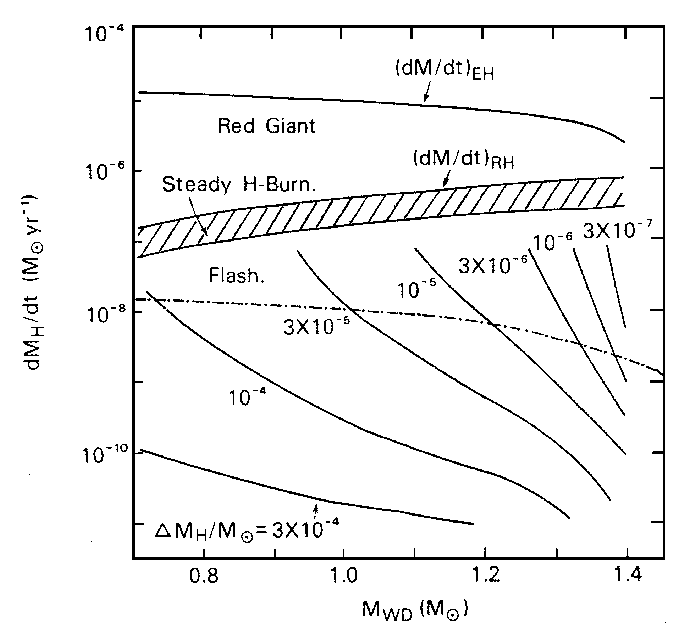
\includegraphics[scale=1.2]{sss-regimes.eps}
        			\caption{Regimes of nuclear burning in surface layers of a white dwarf}
        			\label{fig:regimes-wd}
        		\end{center}
        	\end{figure}
        	
        	These regimes are summarized as follows, for a white dwarf with solar mass:        	
        	\begin{enumerate}
				\item \textbf{Stable hydrogen burning:} For accretion rates within a narrow range of $1-4\times 10^{-7}\,M_{\odot}\,yr^{-1}$, the accreted hydrogen undergoes a stable, continuous burning process on the white dwarf's surface. Crucially, this steady burning occurs without causing significant expansion of the white dwarf itself.
				%For mass accretion rate in the narrow range $1-4\times 10^{-7}\,M_{\odot}\,yr^{-1}$, the accreted hydrogen burns steadily, without any significant radius expansion of the white dwarf.
				\item \textbf{Thermonuclear flashes:} When the accretion rate falls below the threshold for stable burning, the accreted hydrogen ignites in a series of thermonuclear flashes. These explosive events are intermittent, with the frequency of flashes decreasing as the accretion rate diminishes. Concurrently, the individual flashes become more energetic and violent under these conditions.
				%For mass accretion rates below the range of steady burning, the accreted matter burns in flashes, i.e. intermittently. With decreasing accretion rates, the frequency of the flashes decreases and the flashes themselves become more violent.
				\item \textbf{Stable hydrogen burning with radius expansion:} If the accretion rate surpasses the upper limit for stable burning, the white dwarf undergoes dramatic expansion, resembling a red giant star. Despite this expansion, hydrogen burning continues steadily within a thin shell surrounding the white dwarf's core. Intriguingly, this process mirrors the growth of degenerate cores in red giant stars, where hydrogen shell burning is also responsible for the expansion.
				%For mass accretion rates above the range of steady burning, the radius expands to red giant dimensions, and the matter continues to burn steadily within a thin shell around the white dwarf. This, incidentally, corresponds to the growth rate of the degenerate core in red giant stars due to the hydrogen shell burning.
			\end{enumerate}
			
			Hachisu et al. (1996) have calculated that when accretion rates onto a white dwarf significantly exceed the threshold for stable hydrogen burning, a fundamental transformation occurs. Instead of maintaining a static envelope, the accreting matter is expelled in a powerful stellar wind, reaching velocities of approximately 5000 km/s \cite{hachisu96}. Crucially, this high-speed outflow is opaque to soft X-rays, preventing their escape. Consequently, to be observed as a luminous supersoft X-ray source (SSS), the white dwarf must maintain an accretion rate within the stable hydrogen burning regime.
			
			Under these conditions of sustained hydrogen burning, the white dwarf gradually accretes helium while increasing its overall mass. Hachisu et al. suggest that this process can continue until the white dwarf reaches a critical mass of approximately $1.38\,M_{\odot}$, at which point a Type Ia supernova is triggered. This theoretical framework establishes a compelling suggestion of \textit{SSS being the potential progenitors of Type Ia supernovae}.
			%Calculations by Hachisu \emph{et al.} show that when the mass accretion rates are very high, much beyond the steady-burning range, a stellar wind solution replaces the static envelope solution \cite{hachisu96}. This stellar wind flows out from the white dwarfs at high speeds ($\sim 5000$ km/s). Because this stellar wind is opaque to soft X-rays, such radiation do not escape. So long the accretion rate remains within steady-burning range, the white dwarf will be observed as a steady, luminous SSS. According to Hachisu \emph{et al.}, the white dwarf steadily burns hydrogen and accretes helium, thereby increasing its mass up to $1.38\,M_{\odot}$ and then explode as an SN Ia. Therefore, there is a strong suggestion that \emph{SSS could be a possible progenitor for SN Ia}.
		
		\subsection{Possible Companions to a White Dwarf in SSS} \label{introduction:current_status:wd-companions}
			Understanding the nature of the companion star in an SSS system is crucial for elucidating the system's evolutionary history and the mechanisms driving its X-ray emission. This section explores two primary categories of companion stars found in SSS: near main-sequence stars more massive than the white dwarf and symbiotic systems.
		
			\subsubsection{Near main-sequence stars more massive than WDs}
				The simplest configuration for a luminous SSS involves a binary system comprising a white dwarf and a more massive companion star with a radiative envelope, exceeding approximately $1.3\,M_{\odot}$. Once mass transfer from the donor star to the white dwarf commences due to Roche lobe overflow, the binary orbit undergoes shrinkage. The donor star experiences thermal instability, leading to sustained mass transfer until its mass becomes lower than that of the white dwarf, at which point the orbital separation increases \cite{paczynski71}. These systems are termed close-binary supersoft sources (CBSS). Greiner has identified and catalogued\footnote{\url{http://www.mpe.mpg.de/~jcg/sss/ssscat.html}} nine such systems, providing observational support for this model \cite{greiner2000catalog}.
				%The simplest binary configuration that can become a luminous SSS comprises of a white dwarf with a companion star whose mass is larger than about $1.3\,M_{\odot}$ and has a radiative envelope. In such a system, once the donor star overflows its \emph{Roche lobe}, mass transfer to the white dwarf starts, causing its orbit to shrink. The donor becomes thermally unstable and it will continue transferring mass until it becomes less massive of the two and further mass transfer leads to the orbit expansion (Paczynski) \cite{paczynski71}. Such systems are called \emph{close-binary supersoft sources} (CBSS). Nine CBSS have been identified by Greiner \cite{greiner2000catalog,greiner2000catalogOnline}.
				
			\subsubsection{Symbiotic systems}
				Sion et al. (1994) first identified symbiotic systems as another potential host environment for SSS. These systems consist of a white dwarf accreting matter from a red giant companion star. The specific characteristics of the mass transfer process in symbiotic systems can vary depending on the evolutionary stage of the red giant \cite{sion94}. Two primary subtypes of symbiotic SSS are commonly recognized, that provide different modes of mass-transfer.
				%Sion \emph{et al.}\cite{sion94} first showed that a system consisting a red-giant star and a white dwarf is another class of binary systems which can sustain the mass accretion rates necessary for producing supersoft X-rays. Two types of red-giant companions may be expected, providing different modes of mass-transfer.
				
				\begin{enumerate}
					\item One subtype of symbiotic supersoft X-ray sources involves a $1\,M_{\odot}$ red giant companion that is less massive than the white dwarf. These systems typically exhibit orbital periods exceeding 125 days. The red giant component in such systems possesses a degenerate helium core, and its evolutionary processes drive the mass transfer onto the white dwarf. This mass transfer is facilitated by Roche lobe overflow.
					%$1\,M_{\odot}$ red-giant, less massive than the white dwarf. Such a companion overflows its Roche lobe with an orbital period of at least 125 days. The red-giant has a degenerate He core, and its nuclear evolution drives the mass transfer.
					\item Symbiotic systems can also involve a red giant companion in the asymptotic giant branch (AGB) phase of its evolution. Unlike the first subtype, these AGB stars do not fill their Roche lobes. However, they exhibit intense stellar winds, characterized by mass loss rates of the order of $10^{-5}\,M_{\odot}\,yr^{-1}$ and velocities around 30 km/s. A fraction of this ejected material is captured by the white dwarf companion, resulting in accretion rates of about $10^{-7}\,M_{\odot}\,yr^{-1}$. These accretion rates are sufficient to power the white dwarf as a luminous supersoft X-ray source.
					%The red-giant is on the aymptotic giant branch (AGB) and is not filling its Roche lobe, however there is a very strong stellar wind. With mass loss rates from the AGB of the order $10^{-5}\,M_{\odot}\,yr^{-1}$ and stellar wind velocities of around 30 km/s, the aggregate accretion rate can become as large as of the order $10^{-7}\,M_{\odot}\,yr^{-1}$ on a white dwarf, which is sufficient to create a luminous SSS.
				\end{enumerate}
		
		\subsection{Classification Scheme for SSS} \label{introduction:current_status:sss-classification}
			As per di Stefano \emph{et al.} (1996) \cite{distefano96}, binary systems that may appear as luminous SSS may be classified as per table \ref{tab:SSS-class}.
			
			In table \ref{tab:SSS-class}, [A] only those systems are considered in which H-rich material is accreting on the surface of a C-O white dwarf. Here CV = cataclysmic variable, CBSS = close-binary supersoft source and WBSS = wide-binary supersoft source. [B] Two prominent mass transfer mechanisms are mb = magnetic braking and gr = gravitational radiation. [C] $\dot{M}$ is the mass accretion rate on the surface layers of the white dwarf. [D] $P_\text{orb}$ refers to the orbital period of the binary. [D] When $\dot{M}$ is in the correct range (about $\gtrsim 10^{-7}\,M_{\odot}$ yr$^{-1}$), the source burns nuclear fuel more or less steadily (S); for smaller values of $\dot{M}$, hydrogen burns sporadically (R).
			
			\begin{table}[!htb]
				\centering
				\caption{Classification of binary systems that may manifest as SSS}
				\label{tab:SSS-class}
				\begin{tabulary}{\textwidth}{CCCCC}
					\hline
					\small{\textbf{[A] System Type}} & \small{\textbf{[B] Mass Transfer Mechanism}} & \small{\textbf{[C] Mass Accretion Rate $\boldsymbol{\dot{M}}$ ($\boldsymbol{M_{\odot}}$ yr$^{-1}$)}} & \small{\textbf{[D] Orbital Period $\boldsymbol{P}_\text{\textbf{orb}}$ (days)}} & \small{\textbf{[E] Steady or Recurrent}}\\
					\hline
					\small{CVs} & \small{mb and/or gr} & \small{$\lesssim 10^{-8}$} & \small{$\lesssim 0.2$} & \small{R}\\
					\hline
					\small{CBSSs} & \small{thermal time scale readjustment of donor} & \small{$\gtrsim 10^{-7}$} & \small{$\sim 0.2-3.0$} & \small{S}\\
					\small{} & \small{} & \small{$\lesssim 10^{-7}$} & \small{$\sim 0.2-\mathscr{O}(10^2)$} & \small{R}\\
					\hline
					\small{WBSSs} & \small{nuclear evolution of donor} & \small{$\gtrsim 10^{-7}$} & \small{$\sim 3.0-\mathscr{O}(10^2)$} & \small{S}\\
					\small{} & \small{} & \small{$\lesssim 10^{-7}$} & \small{$\sim 3.0-\mathscr{O}(10^2)$} & \small{R}\\
					\hline
					\small{Symbiotics (Wind-driven)} & \small{stellar winds from evolved donor} & \small{$\gtrsim 10^{-7}$} & \small{$\mathscr{O}(10^2)$} & \small{S}\\
					\small{} & \small{} & \small{$\lesssim 10^{-7}$} & \small{$\mathscr{O}(10^2)$} & \small{R}\\
					\hline
				\end{tabulary}
			\end{table}
			
		\subsection{Classical Novae} \label{introduction:current_status:CNe}
			Classical novae rank as the third most cataclysmic explosions within a galaxy, surpassed only by supernovae and gamma-ray bursts in terms of energy release. While novae are far less energetic than supernovae, typically liberating luminosities of more than $10^{45}$ erg s$^{-1}$, they occur with significantly higher frequency, making them more commonly observed phenomena within galactic environments.
			%Classical nova explosions are regarded as the third most violent explosions that can occur in a galaxy, preceded by a supernova explosion and a $\gamma$-ray burst. With total liberated energies of more than $10^{45}$ erg s$^{-1}$, novae are less energetic than supernovae, but far more frequent within a galaxy.
			
			The prevailing model for classical novae, as outlined by Krautter (2008), posits their occurrence within cataclysmic binary systems. These systems comprise a white dwarf primary accreting matter from a main-sequence or slightly evolved companion star. The mass transfer process, facilitated by Roche lobe overflow, channels material towards the white dwarf through the inner Lagrangian point, forming an accretion disk.
			
			The conditions leading to a thermonuclear runaway on the white dwarf's surface are intricately linked to factors such as the white dwarf's mass and luminosity, the accretion rate, and the chemical composition of the accreted material \cite{starrfield89}. As hydrogen-rich matter accumulates, it undergoes compression and heating. When temperatures within the accreted layer surpass $10^8$ K, runaway thermonuclear fusion ignites, releasing vast amounts of energy. The peak luminosity during these events can approach the Eddington limit $L_\text{Edd}$, a critical threshold beyond which radiation pressure exceeds gravitational force, imposing an upper limit on the luminosity of a star.
			%As per the accepted standard model described by Krautter, nova explosions occur in cataclysmic binary systems \cite{krautter08}. In such systems, one member is a white dwarf and the other member is a main-sequence or slightly evolved star that fills its Roche lobe, with mass transfer from the secondary to the white dwarf taking place through the inner Lagrangian point, leading to the formation of an accretion disk. The evolution of a thermonuclear runaway on the white dwarf depends upon the mass and luminosity of the white dwarf, the mass accretion rate, and the chemical composition of the accreted layer \cite{starrfield89}. The temperature in the H-burning zone can grow to values exceeding $10^8$ K, while luminosities are of the order of the Eddington luminosity $L_\text{Edd}$ (\textit{Eddington luminosity}, or \textit{Eddington limit}, is the maximum luminosity a body can achieve under the state of \textit{hydrostatic equilibrium}).
			
			X-ray observations have emerged as a pivotal tool for investigating the high-temperature phases associated with nova outbursts.
 While these observations have yielded valuable insights, the relatively small number of novae studied in the X-ray band compared to other spectral domains (optical, infrared, ultraviolet) has hindered the development of a comprehensive understanding of novae in this energy range. Nevertheless, two primary mechanisms have been proposed to explain X-ray emission from novae.
			%X-ray astronomy has turned out to be a powerful tool for the study of novae outburst, since the X-ray regime is best suited to study such hot phases. X-ray observations have provided many fundamental and in part unexpected results. However, so far the picture that emerged from X-ray observations of novae is far less systematic than the one from other spectral regimes, since unlike in the optical, infrared, or ultraviolet regime, only few objects were observed in X-rays.
			
			%Two viable mechanisms for X-ray emission from a nova outburst are described in brief here.
			
			\subsubsection{Thermal radiation from hot white dwarf}
				Following a nova eruption, the energy released from thermonuclear burning is rapidly transported to the white dwarf's surface. This influx of energy dramatically increases the star's effective temperature. For a white dwarf radiating at its Eddington luminosity $L_\text{Edd}$, the temperature could be expected to be several thousand kelvins, depending on the white dwarf's mass. Consequently, the nova enters a phase of intense soft X-ray emission, characterized by a spectral energy distribution (SED) resembling that of a hot stellar atmosphere.
				
				As the nova ejecta expand outward, they form a cooling pseudo-photosphere. This expansion leads to a rapid decrease in temperature and a corresponding decline in X-ray flux due to the increasing opacity of the expanding envelope to X-rays \cite{krautter96}.
				%After the energy created by nuclear reactions has reached the surface of the white dwarf, the effective surface temperature increases rapidly.For luminosity of the order of $L_\text{Edd}$ and unit white dwarf radius, the temperature could be expected to be several thousand kelvins (depending on the white dwarf mass). The nova then emits strong soft X-rays with the \emph{spectral energy distribution} (SED) of a hot stellar atmosphere. After the ejection of the nova shell, the temperature of the expanding pseudo-photosphere decreases rapidly with increasing radius. Also, the X-ray flus drops since the expanding envelope becomes opaque to X-rays (Krautter \emph{et al.}) \cite{krautter96}.
				
			\subsubsection{X-ray emission from circumstellar material}
				A second mechanism contributing to X-ray emission in nova systems involves interactions between the expanding nova ejecta and the surrounding circumstellar environment. This interaction can occur either within the ejected material itself or between the ejecta and pre-existing circumstellar matter. As proposed by Balman et al. (1998), shock waves generated by these collisions can reach temperatures of several keV, producing thermal \textit{bremsstrahlung} radiation in the X-ray band \cite{balman98}.
				%In the circumstellar material surrounding the nova system, the expanding nova shell and/or a nova wind interact with pre-existing material of with each other. In this mechanism, as per Balman \emph{et al.} \cite{balman98}, strong shocks giving rise to a thermal \emph{bremsstrahlung} SED with temperatures up to several keV may be expected.

    \section{Statement of the Research Problem} \label{introduction:problem_statement}
    	To understand the nature of binary systems emitting supersoft X-rays by the analysis of their spectra and the study of their variabilities in X-ray and visible/ultraviolet regimes.
        
    \section{Hypothesis} \label{introduction:hypothesis}
    	The radiative processes governing supersoft X-ray sources are much complex than previously assumed and could include non-steady states, NLTE and stellar winds.
    
    \section{Objectives of the Study} \label{introduction:objectives}
    	\begin{enumerate}
    		\item To develop a robust and consistent model that accurately fits the continuum spectra of supersoft X-ray sources (SSS) across different sources, and using multi-observatory science data.
    		
    		\item To demonstrate that the spectra of SSS within the 0.2--1.0 keV photon energy range can be satisfactorily modeled using Non-Local Thermodynamic Equilibrium (NLTE) components, and to validate this approach across multiple sources.
    		
    		\item To investigate and distinguish the absorption components due to the source atmosphere and the interstellar medium (ISM) in the spectra of SSS from both the Milky Way and the Large Magellanic Cloud (LMC).
    		
    		\item To compute stellar parameters for the selected SSS using the best-fit models, thereby constraining their luminosities, effective temperature and column densities.
    		
    		\item To investigate and distinguish the absorption components due to the source atmosphere and the interstellar medium (ISM) in the spectra of SSS from both the Milky Way and the Large Magellanic Cloud (LMC).
    		
    		\item To identify and analyze the differences in spectral characteristics, such as absorption edges, between SSS in the Milky Way and those in the LMC, and to understand the underlying reasons for these differences.
    		
    		\item To develop a software tool that accesses publicly available atomic data and overlays the relevant atomic lines on the grating spectra of SSS, thereby facilitating preliminary line identification for astronomers.
    		
    		\item To study a grid of models for fitting the grating spectra of SSS, comparing their fitting statistics.
    	\end{enumerate}
%    	\begin{enumerate}
%			\item To study different models for spectral fitting of the list of sources.
%			\item To study the temporal variability of the list of sources.
%			\item To propose and calculate novel stellar atmospheric models and generate the associated synthetic spectra.
%			\item To develop corresponding software models that can be used in XSPEC.
%			\item To compute stellar parameters for the list of sources using the best-fit models.
%			\item To propose models for the interstellar medium by studying the absorption edges in the observed spectra of the identified sources.
%		\end{enumerate}
    
    \section{Significance of the Study} \label{introduction:significance}
    	The study of SSS is crucial for understanding the physics and evolution of compact binary systems, such as white dwarfs and their interactions with companion stars. This research addresses several key challenges in modeling the spectra of SSS, providing significant advancements in the field of high-energy astrophysics.
    	
    	Firstly, developing a robust and consistent model that accurately fits the continuum spectra of SSS across different sources and using multi-observatory data is fundamental to obtaining reliable measurements of their physical parameters. This helps in better understanding the nature of these sources, their life-cycle, and their role in the broader context of stellar evolution.
    	
    	Secondly, demonstrating that the spectra of SSS within the 0.2--1.0 keV photon energy range can be satisfactorily modelled using Non-Local Thermodynamic Equilibrium (NLTE) components fills a crucial gap in current astrophysical models. NLTE modeling provides a more accurate representation of the physical conditions in the atmospheres of SSS, leading to more precise determinations of their effective temperatures, luminosities, and column densities. Additionally, the spectra fitted within this range can be extrapolated to lower energies (or higher wavelengths) and compared with observations made in the UV/optical regime. This cross-validation enhances the reliability of the models and provides a comprehensive understanding of the sources across different wavelengths.
    	
    	Thirdly, investigating the absorption components due to the source atmosphere and the interstellar medium (ISM) in the spectra of SSS from both the Milky Way and the Large Magellanic Cloud (LMC) adds another layer of understanding regarding the interaction of X-ray photons with intervening matter. This not only enhances our comprehension of the local environments of these sources but also provides insights into the composition and distribution of the ISM in different galactic environments.
    	
    	Additionally, by computing stellar parameters using best-fit models, the study places constraints on the luminosities, effective temperatures, and column densities of SSS, contributing valuable data to the field of stellar astrophysics. Identifying and analyzing differences in spectral characteristics, such as absorption edges, between SSS in the Milky Way and those in the LMC, sheds light on the unique astrophysical processes at play in different galactic contexts.
    	
    	Furthermore, the development of a software tool for preliminary line identification using publicly available atomic data is a significant contribution to the astronomical community. This tool facilitates the identification of key atomic lines in grating spectra, enabling more detailed and accurate spectral analysis.
    	
    	Finally, by studying a grid of models for fitting the grating spectra of SSS and comparing their fitting statistics provides a comprehensive evaluation of different modeling approaches, ensuring the selection of the most appropriate models for accurate spectral fitting.
%        Different observations of SSS, separated from each other by months, exhibit new SSS and, more importantly, only a few members which are common to previous observations. This clearly implies that such sources have ``on/off'' phases that take place over time intervals spanning months. It is indeed certain that, with continuous monitoring of SSS over time-frames in decades, the number of SSS discovered would increase dramatically.
%        
%        Study of the X-ray variability of SSS is expected to provide valuable clues to the dynamics of the SSS -- not only for those already well-studied, but also for newly-discovered sources for which satisfactory models are yet to be arrived at. Simultaneously, the study of the features present in their spectra, using robust models, promises to shed light on the physics behind the processes taking place in SSS. In addition, a careful study of the absorption edges, due to various metals, exhibited in their high-resolution spectra can provide clues to the structure and composition of the intervening interstellar medium.
%        
%        Our present understanding of nuclear-burning white dwarfs and progenitors of type Ia supernovae explosions can evolve significantly with further monitoring and study of SSS. The reason for this being the fact that these are observed to be accompanied by a phase of supersoft X-ray emission.
    
    \section{Contribution of the Thesis} \label{introduction:thesis_contribution}
    	The current thesis makes several important contributions to the field of high-energy astrophysics, particularly in the study of supersoft X-ray sources:
    	\begin{enumerate}[I.]
    		\item \textbf{Development of a Robust Spectral Model:} The current thesis presents a robust and consistent model that accurately fits the continuum spectra of SSS across different sources using data from multiple observatories. This model provides a reliable framework for analyzing and interpreting SSS spectra.
    		
    		\item \textbf{Validation of NLTE Modeling:} By demonstrating that the spectra of SSS within the 0.2--1.0 keV photon energy range can be satisfactorily modeled using NLTE components, this research validates a crucial approach for studying the physical conditions in the atmospheres of these sources. This contributes to more accurate determinations of their temperatures and luminosities. Moreover, the extrapolation of these models to UV/optical observations strengthen the consistency and reliability of the models.
    		
    		\item \textbf{Analysis of Absorption Components:} The investigation into the absorption components due to the source atmosphere and the ISM in the spectra of SSS from both the Milky Way and the LMC provides a deeper understanding of the interactions between X-ray photons and intervening matter. This analysis enhances our knowledge of the local environments of SSS and the ISM's composition in different galaxies.
    		
    		\item \textbf{Computation of Stellar Parameters:} The thesis provides precise computations of stellar parameters for the selected SSS, including luminosities, effective temperatures, and column densities. These results are valuable for constraining models of these sources and understanding their physical properties.
    		
    		\item \textbf{Identification of Spectral Absorption Edges:} By identifying and analyzing differences in absorption edges, between SSS in the Milky Way and those in the LMC, the research offers insights into the unique astrophysical processes in different galactic environments. This helps explain the variations in the observed spectra of SSS.
    		
    		\item \textbf{Development of a Line Identification Tool:} The development of a Python-based software tool\footnote{\url{https://github.com/pararover/xmmrgs_lines}} that accesses atomic data and overlays relevant atomic lines on the grating spectra of SSS is a practical contribution. This tool aids astronomers in performing preliminary line identification, facilitating further spectral analysis and interpretation.
    		
    		\item \textbf{Evaluation of Spectral Models:} By studying a grid of models for fitting the grating spectra of SSS and comparing their fitting statistics, the thesis provides a comprehensive evaluation of different modeling approaches. This ensures the selection of the most suitable models for accurate spectral fitting, enhancing the reliability of spectral analysis.
    	\end{enumerate}
        %The present study obtains an unprecedented model fit of the complex high-resolution spectrum of the source named \mrvel\ with the RGS instrument of the XMM-Newton observatory. In the process, we propose a hypothesis for the physical processes that govern the radiation from this particular X-ray binary. We also apply a similar spectral study on other supersoft X-ray sources with similar spectral characteristics.
    
    %\section{Organization of the Thesis} \label{introduction:thesis_organization}
    %    \lipsum[10]
		% COMPLETE
    \chapter{MULTI-OBSERVATORY SPECTRAL ANALYSIS OF SUPERSOFT X-RAY SOURCES} \label{chap:multi-obs}
    %\doublespacing
    \minitoc
    
    \newpage
    \begin{center}
    	\emph{Abstract of chapter \ref{chap:multi-obs}}
    \end{center}
    
    In this chapter, we present a comprehensive study on the spectral characteristics and parameters of the supersoft X-ray source \source. We utilize a dataset comprising of six observations conducted by four different space observatories, namely ASCA, Chandra, XMM-Newton and NICER, spanning a time period of 25 years. Our objective is to identify a robust NLTE spectral model that can provide an acceptable fit to the continuum spectrum of \source, which had not been performed earlier as per current literature, thereby enhancing our understanding of its astrophysical nature. The study employs rigorous spectral modeling and comparative analysis to establish a framework for characterizing the continuum spectrum of \source. The study also discusses the analysis of the supersoft spectrum of \source, including the challenges in reproducing its spectra using NLTE model atmospheres. The best-fit model consists of a pure hydrogen NLTE model with effective gravity of 7, in conjunction with photoelectric absorption, ISM absorption and edge components. The effective temperature is found to be approximately of the order of $\sim 10^5$ K for all six observations, suggesting the presence of a hot accretion disk surrounding the white dwarf, which accretes matter from a companion main-sequence star. The study also analyzes the relative strengths of absorption edges in the spectrum and notes inconsistencies in the NICER observations. {The current work demonstrates that while the continuum spectrum of \source\ can be fitted satisfactorily, the same cannot be said to be the case for its high-resolution grating spectra. Therefore, it makes a case for the need to explore and develop methods that study such latest grating spectra, so as to obtain a more nuanced view of the astrophysics involving \source.}
    
    \section{Literature Review} \label{multi-obs:lit-rev}
    	Supersoft X-ray sources (SSS) represent an important class of celestial objects. They were initially recognized as a distinct class of intrinsically luminous X-ray sources by Trümper \textit{et al.} \cite{trumper1991x}, Greiner \textit{et al.} \cite{greiner1991rosat}, and Kahabka \textit{et al.} \cite{kahabka97}. These sources are classified based on their X-ray luminosities, which are typically around the Eddington limit ($\sim 10^{38}$ erg s$^{-1}$), indicating their exceptionally high brightness. However, their defining feature is their extremely soft X-ray spectra, with weak or negligible emission beyond $\sim 1$ keV and effective blackbody temperature no more than $\sim 100$ eV (or $\lesssim 1200$ kK) \cite{kahabka06}. The understanding of the spectral characteristics of SSS promises to pave the way for a deeper exploration of their role in the broader astrophysical landscape.
    	
    	SSS were initially observed by the Einstein Observatory during a soft X-ray survey of the Large Magellanic Cloud (LMC) by Long et al. in 1981 \cite{long81}. Over time, hundreds of objects exhibiting similar characteristics have been documented, many of which are considered candidates or confirmed members of this class. The catalog of SSS has expanded significantly, now encompassing sources not only within the LMC but also various other celestial bodies, including the Milky Way (MW), Small Magellanic Cloud (SMC), and Andromeda (M31) and numerous other galaxies \cite{kahabkatrumper1996,steinerdiaz1998,greiner2000,pietsch2003deep,di2003luminous,orio2010census,henze2010recent,sturm2012new,galiullin2021populations}.
    	
    	The relatively fewer detections of SSS within our galaxy, compared to other galaxies, may be attributed to significant interstellar extinction of soft X-rays. Situated at the edge of the MW and along its galactic plane, soft X-rays emitted by galactic SSS face considerable interstellar absorption. Suggestions have been made that SSS within the galactic plane must be within a distance of approximately 1 kpc to remain observable. Beyond this distance, interstellar absorption becomes sufficiently pronounced to render them undetectable \cite{van1992accreting}.
    	
    	The optical spectra of the SSS in the Magellanic Cloud galaxies exhibit similarities with those of low-mass X-ray binaries -- characterized by strong emission lines such as He II at 4686 \AA\ and hydrogen Balmer lines. Subsequent numerical calculations suggested that SSS could result from near-Eddington accretion onto neutron stars \cite{kylafis93}, although subsequent analyses favoured white dwarfs as the emitting objects for supersoft X-rays \cite{vandenHeuvel92}.
    	
    	Employing Stefan-Boltzmann's law with typical luminosity and effective temperature values for SSS, the estimated radius of the emitting object aligns with that of a white dwarf, supporting the hypothesis of accretion onto white dwarfs as the source of supersoft X-rays, akin to accreting neutron stars and black holes in classical X-ray binaries. Van den Heuvel proposed that white dwarfs with masses in the range $0.7–1.4\,M_\odot$ and mass accretion rates $\sim 1-5\times 10^{-7}\,M_\odot\text{ yr}^{-1}$ produce supersoft X-rays, assuming the mass-accretor as the white dwarf and the companion as a main-sequence or post-main-sequence star within specific mass ranges \cite{van1992accreting}. Studies by various groups have explored different types of nuclear burning due to mass accretion on white dwarfs, depending on the thermal history of the white dwarf and conditions required for nuclear ignition, typically involving critical envelope masses %$\Delta M_\text{crit}$
    sustaining high temperatures ($\sim 10^8$ K) and pressures ($\gtrsim 10^{18}-10^{20}$ g cm$^{-1}$ s$^{-2}$) for nuclear burning via the CNO cycle \cite{paczynski78,prialnik78,sion79,sienkiewicz80,nomoto82,fujimoto82a,fujimoto82b,iben82,prialnik95,macdonald83}. The steady state accretion rate, crucial for understanding the relationship between accretion and nuclear burning, has been investigated in early calculations \cite{paczynski80,iben82}, providing insights into the dynamics of hydrogen-rich matter accretion on white dwarfs. For a hydrogen-rich system, the steady state accretion rate was given to be \cite{hachisu2001}
		\begin{align}
			\dot{M}_\text{steady}\sim 3.7\times 10^{-7}\left( \dfrac{M_\text{WD}}{M_\odot}-0.4 \right)\,M_\odot\,\text{yr}^{-1} \label{eqn:steady-mass-accr}
		\end{align}
	
		The particular luminous galactic SSS known as MR Vel, and referred to as \source, was discovered by Motch \textit{et al.} \cite{motch1994} in the ROSAT Galactic Plane Survey (RGPS), which  is defined as the $|b|\leqslant 20\degree$ region of the ROSAT All Sky Survey. In the J2000 frame, the right ascension and declination of \source\ is 141.44042 and -47.96972 ($\alpha$=09 25 46.00, $\delta$=-47 58 17.4: as resolved by Simbad\footnote{\url{http://simbad.u-strasbg.fr/simbad/}}).
		
		\source\ was the brightest SSS candidate source in RGPS, with ROSAT PSPC hardness ratios of $HR1=0.96\pm 0.03$ and $HR2=-0.69\pm 0.03$. Fitting a blackbody to the ROSAT observations, a hydrogen column density in the range $n_H=(1.4-3.7)\times 10^{22}$ cm$^{-2}$ can be obtained. There is a considerable amount of uncertainty in current literature about its distance, with estimates ranging from 1 kpc to 10 kpc. Consulting Gaia Data Release 3\footnote{\url{https://www.cosmos.esa.int/web/gaia/data-release-3}}, one can find negligible parallax. This fact along with its high luminosity suggests that its distance is likely to be $>5$ kpc.
		
		Hartmann \textit{et al.} applied non-local thermodynamic equilibrium (NLTE) models, which included metal line opacities, to the spectrum extracted from the observations by BeppoSAX LECS of RX J0925 on January 25-26 1997 \cite{hartmann1999constraining}. They found that if a single model component is assumed for \source, a large discrepancy is observed between the model and data above 1.19 keV. The emission above $\sim 1.2$ kev (i.e. Ne IX edge) can be accounted for by adding another spectral model component, namely collisional ionization equilibrium.
		
		Higher resolution data obtained using the grating instruments on-board the Chandra and XMM-Newton observatories revealed complex structures in the spectra of \source. Such spectra show the presence of P Cygni profiles of Fe XVII and O VIII, which typically arise in a wind. Earlier, Bearda et al. (2002) and Motch et al. (2002) had come to the conclusion that the \source\ spectra, as observed by the Chandra HETGS and the XMM-Newton RGS, cannot be reproduced by LTE or NLTE model atmospheres \cite{beardaChandra2002AA,motchXmmNewton2002AA}, even though there is little clarity on the reason for this. Obtaining an acceptable fit for \source\ spectrum assumes crucial importance at this juncture. In the absence of a proper model describing the emission spectrum, it becomes impossible to calculate its parameters such as effective temperature and luminosity.
		
		In the present work, our primary objective was to identify a robust spectral model capable of providing an acceptable fit to the continuum spectrum of \source. To this end, we devised an approach wherein we analyse spectral data for \source\ obtained using multiple observatories. A motivation for harnessing such multi-observatory science data over an extended period was to mitigate potential biases associated with individual instruments and temporal variations in observational conditions, thereby enabling a systematic examination of the source's spectral characteristics, in an attempt to constrain the underlying physical processes driving the observed supersoft X-ray emission.
		
		The amalgamation of observations from diverse space observatories offered unique insights into the spectral evolution of the supersoft X-ray source over time, shedding light on its dynamic behavior and emission properties. Through rigorous spectral modeling and comparative analysis, we made an attempt to establish a robust framework for characterizing the continuum spectrum of the supersoft source, thereby enhancing our understanding of its astrophysical nature and evolutionary trends. A comprehensive investigation into recurrent SSS like \source\ is paramount due to the emerging recognition of SSS as progenitors of type Ia supernovae, which serve as crucial standard candles in cosmology. By delving deeper into the astrophysical mechanisms governing SSS, we can potentially enhance our ability to make precise predictions regarding the occurrence of type Ia supernovae and subsequently refine cosmological distance measurements.
    
    \section{Journal of Observations} \label{multi-obs:journal}
    	During the course of our investigation of the continuum spectrum of \source, we leveraged a comprehensive dataset comprising six observations conducted by four distinct space observatories spanning the years 1994 to 2019. We extracted spectral data within the range 0.2 -- 1.0 keV from each observation in this dataset. This afforded us the opportunity to apply a consistent spectral analysis approach across a broad temporal range and disparate instrumentation platforms.
    	
    	A summary of the observations used in this study, which included science data from Japan's ASCA \cite{ebisawaAsca2001ApJ}, NASA's Chandra \cite{beardaChandra2002AA}, ESA's XMM-Newton \cite{motchXmmNewton2002AA} and ISS' NICER \cite{orioNicer2022ApJ} observatories, is presented in table \ref{tab:obs-journal}.
    	
    	\begin{landscape}
    	\renewcommand{\arraystretch}{2.2}
    	\begin{table}[!htb]
	    	\centering
	    	\caption{Journal of observations}
	    	\label{tab:obs-journal}
			\begin{tabular}{ccccccc}
				\hline
				\textbf{\begin{tabular}[c]{@{}c@{}}Observation\\ (Obs. ID)\end{tabular}} & \textbf{\begin{tabular}[c]{@{}c@{}}Date\\ (yyyy-mm-dd)\end{tabular}} & \textbf{Observatory} & \textbf{Instrument} & \textbf{MJD}$^\dagger$ & \textbf{\begin{tabular}[c]{@{}c@{}}Exposure$^\ddagger$\\ (ks)\end{tabular}} & \textbf{Region (keV)} \\
				\hline
				{43036000}   & {1994-12-22} & {ASCA} & {SIS1}          & {49708.56} & {20.58} & {0.20--1.00} \\
				{644}        & {2000-11-14} & {Chandra} & {ACIS}       & {51862.92} & {57.40} & {0.40--1.00} \\
				{0111150101} & {2000-12-16} & {XMM-Newton} & {EPIC-pn} & {51894.46} & {61.10} & {0.30--1.00} \\
				{2611020101} & {2019-05-18} & {NICER} & {XTI}          & {58621.90} & {2.53} & {0.40--1.00}  \\
				{2611020102} & {2019-05-19} & {NICER} & {XTI}          & {58622.03} & {8.57} & {0.45--1.00}  \\
				{2611020103} & {2019-05-19} & {NICER} & {XTI}          & {58623.00} & {9.91} & {0.45--1.00}  \\
				\hline
			\end{tabular}
			
			\begin{minipage}{16cm}
				\vspace{0.1cm}
				\small $^\dagger$Modified Julian Date
				
				\small $^\ddagger$From HEASARC archival query results
			\end{minipage}
		\end{table}
		\renewcommand{\arraystretch}{1.6}
		\end{landscape}
    
    \section{Data Reduction and Analysis} \label{multi-obs:red-analysis}
    	The raw data pertaining to all of the observations were downloaded using the online archival query interface at the \textit{High Energy Astrophysics Science Archive Research Center} (HEASARC)\footnote{\url{https://heasarc.gsfc.nasa.gov/db-perl/W3Browse/w3browse.pl}}. The data was reduced finally to \textit{Flexible Image Transport System} (FITS)\footnote{\url{https://fits.gsfc.nasa.gov/standard40/fits_standard40aa-le.pdf}} format using the software tools for the corresponding observatory with recommended settings in the relevant data analysis threads, wherever available. For the final analysis, a set of four files were generated for each of the observations. As a standard practice, these files were given the extensions as per a convention adopted by the authors as follows:
	    \begin{enumerate}
	    	\item Source spectrum, with file extension \texttt{.src}
	    	\item Background spectrum, with file extension \texttt{.bkg}
	    	\item Redistribution matrix file (RMF), with file extension \texttt{.rmf}
	    	\item Ancillary response file (ARF), with file extension \texttt{.arf}
	    \end{enumerate}
	    The above files were grouped using the FTOOLS task \texttt{grphha}\footnote{\url{https://heasarc.gsfc.nasa.gov/docs/heasarc/caldb/docs/memos/cal_sw_93_010/cal_sw_93_010.pdf}} to have an appropriate minimum number of counts per bin. The resulting spectrum sets were analysed using \textit{XSPEC} version 12.13.1.
    
    	\subsection{XMM-Newton EPIC-pn Data Reduction} \label{multi-obs:red-analysis:epic-pn}
    		The SSS \source\ was observed by all the instruments, viz. EPIC-MOS 1, EPIC-MOS 2, EPIC-pn and RGS, on-board ESA's XMM-Newton observatory for $\sim 52$ ks on 16 December 2000. Whereas, we had retrieved data from all the instruments, we decided to use only the EPIC-pn data. The reason for this being two-fold:
	    	\begin{enumerate}[i.]
	    		\item The spectral region of interest is of the lowest energies detectable by EPIC, and the pn detector has a comparatively higher sensitivity than the MOS detectors at lower energies \cite{stecchini2023revisiting,mateos2009statistical}.
	    		\item Currently, the high resolution grating spectra (such as those produced by the RGS) yield unacceptable fits to atmosphere models of SSS. Also, no atmosphere model has yet been able to reproduce all the details in such grating spectra \cite{ness2020complications}.
	    	\end{enumerate}
	    	As per recommendations by the XMM-Newton SOC, the data analysis was restricted to energies above 0.2 keV\footnote{\url{https://xmmweb.esac.esa.int/docs/documents/CAL-TN-0018.pdf}}. The data reduction procedures were performed using the \textit{XMM-Newton Science Analysis System} (SAS) version 21.0.0.
	    
	    	The Observation Data Files (ODF) were downloaded from HEASARC. In order to prepare the data for processing, we included the instrumental and calibration information by creating a Calibration Index File (CIF), which was up-to-date with the current calibration files (CCF)\footnote{\url{https://www.cosmos.esa.int/web/xmm-newton/current-calibration-files}}, and an extended ODF summary file. These were done by running the SAS tasks \texttt{cifbuild} and \texttt{odfingest} respectively. The ODFs were then reprocessed to generate the calibrated event files using the \texttt{epproc}, using the default parameters. The event file for EPIC-pn was filtered using the canned screening set of flags, and by setting \texttt{PATTERN==0} to select only single-pixel events in order to maximise energy calibration and resolution. The procedure described by Jethwa et al. (2015) \cite{jethwa2015pile} was used to check and find that the spectral distortion and flux loss both $<0.01\%$, which implied that the pile-up effects could be neglected.
	    	\begin{figure}[!htb]
		        \centering
		        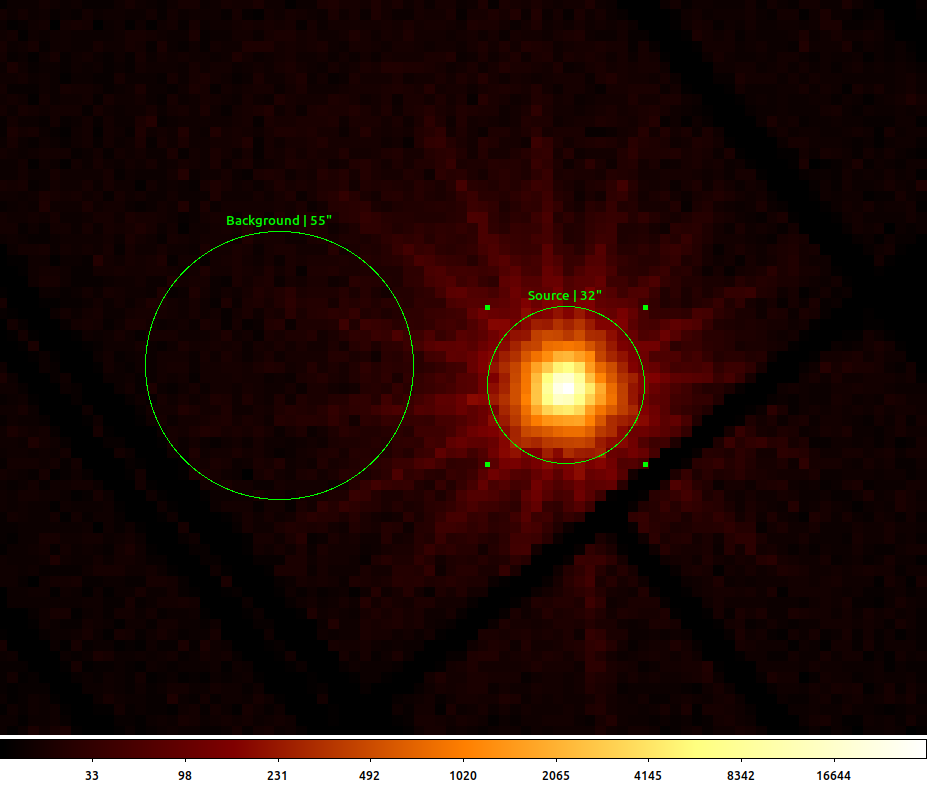
\includegraphics[width=0.8\textwidth]{images/rx-j0925-7-4758_0111150101_src-bkg.png}
		        \caption{Source and background extraction regions for the XMM-Newton observation of \source}
		        \label{fig:src-bkg:pn}
		    \end{figure}
		    
		    The source photons were idensified using DS9 and extracted from a circular region having a radius of 30" which is centred at the \source\ centroid position, encompassing about 85-90\% of XMM-Newton's telescope's on-axis PSF\footnote{\url{https://xmm-tools.cosmos.esa.int/external/xmm_user_support/documentation/uhb/onaxisxraypsf.html}}. For the background photons, first the SAS task \texttt{ebkgreg} was executed to obtain an optimum circular background extraction region of radius $\sim$55". The resulting source and background extraction regions are displayed in figure \ref{fig:src-bkg:pn}. The RMF and ARF were generated using the standard SAS tasks \texttt{rmfgen} and \texttt{arfgen}. The spectrum was finally binned to have a minimum of 10 counts/bin using the task \texttt{grphha} in order to make it ready for analysis using XSPEC.

    	
    	\subsection{ASCA SIS1 Data Reduction} \label{multi-obs:red-analysis:sis1}
    		\source\ was observed by the SIS1 instrument on-board Japan's ASCA observatory for a total duration of $\sim 21$ ks on 22 December 1994, with the purposes of characterization of its continuum spectral shape and the investigation of absorption edge features \cite{ebisawaAsca2001ApJ}. Because SIS1 has greater effective area for energies $<1.5$ keV\footnote{\url{https://heasarc.gsfc.nasa.gov/docs/asca/newsletters/sis_overview.html}}, the data analysis was restricted to an energy range of 0.2-1.0 keV. The procedures for the extraction of spectra were performed using \textit{XSELECT}\footnote{\url{https://heasarc.gsfc.nasa.gov/ftools/xselect/}} version 2.5, a multipurpose tool for filtering event files and generating images, spectra, and light curves made available as part of HEASoft.
    	
    		The event files were downloaded from HEASARC. They were loaded into XSELECT and the source and background spectra were extracted using a circular region of radius 127" and an annular region of radii 129" and 210" respectively, centred at \source\ centroid position. The RMF and ARF were generated using the FTOOL tasks \texttt{sisrmg}\footnote{\url{https://heasarc.gsfc.nasa.gov/lheasoft/ftools/fhelp/sisrmg.html}} and \texttt{ascaarf}\footnote{\url{https://heasarc.gsfc.nasa.gov/lheasoft/ftools/fhelp/ascaarf.html}} respectively. The spectrum set was grouped and binned to a minimum of 20 counts/bin using \texttt{grppha} so as to analyse using XSPEC.
    	
    	\subsection{Chandra ACIS Data Reduction} \label{multi-obs:red-analysis:acis}
    		\source\ was observed during 14 November 2000 for a duration of $\sim 57$ ks using the High-Energy Transmission Grating Spectrometer (HETGS) on-board NASA's Chandra X-ray Observatory \cite{beardaChandra2002AA}. The photons were detected with the ACIS-S CCD array at the focal plane. The data analysis was performed in the energy range 0.4--1.0 keV, with 0.4 keV being the lower limit of the HETGS+ACIS-S spectrometer combination. The extraction of the spectrum and response files was performed using \textit{CIAO} version 4.10 and the Chandra calibration database \textit{CALDB} version 4.7.7.
	    	\begin{figure}[!htb]
		        \centering
		        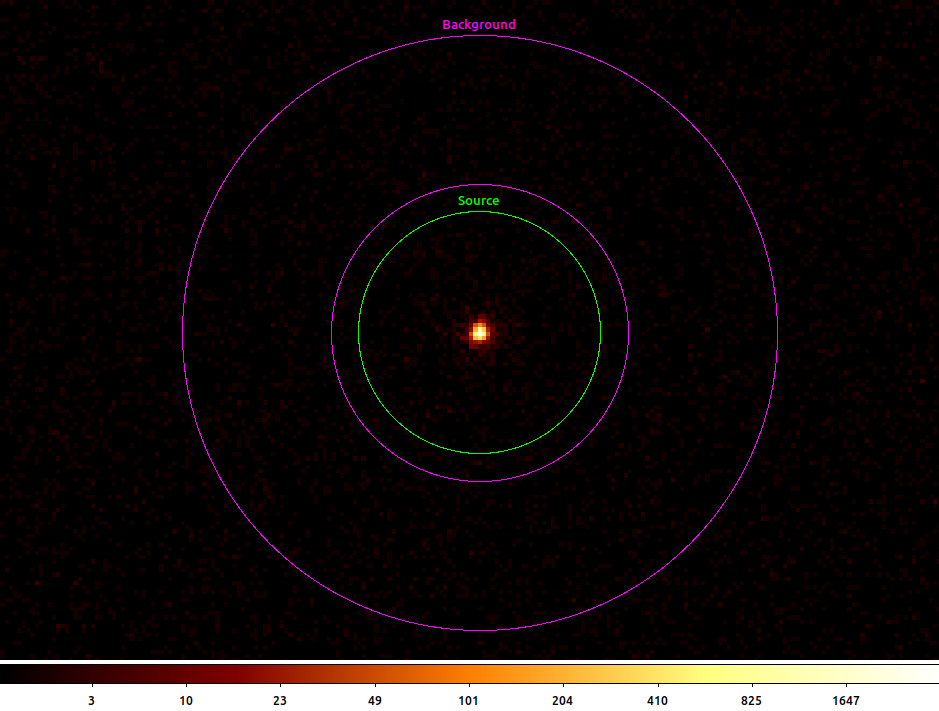
\includegraphics[width=0.8\textwidth]{images/rx-j0925-7-4758_644_src-bkg.png}
		        \caption{Source and background extraction regions for the Chandra observation of \source}
		        \label{fig:src-bkg:acis}
		    \end{figure}
	    	
	    	All the science data files were downloaded from HEASARC. DS9 was used to identify the source and background regions as being a circular region of radius 0.23' and an annular region of radii 0.28' and 0.57' respectively. The source and background spectra were extracted as FITS files using the task \texttt{specextract}\footnote{\url{https://cxc.cfa.harvard.edu/ciao/ahelp/specextract.html}} using standard parameters as per the data analysis threads for point-like sources\footnote{\url{https://cxc.cfa.harvard.edu/ciao/threads/pointlike/}}. The relevant RMF and ARF were generated using the \texttt{mkacisrmf}\footnote{\url{https://cxc.cfa.harvard.edu/ciao/ahelp/mkacisrmf.html}} and \texttt{mkarf}\footnote{\url{https://cxc.cfa.harvard.edu/ciao/ahelp/mkarf.html}} tasks respectively. The spectrum set was grouped and binned to have a minimum of 10 counts/bin using the task \texttt{grphha} for subsequent analysis using XSPEC.
    	
    	\subsection{NICER XTI Data Reduction} \label{multi-obs:red-analysis:xti}
    		\source\ was observed by the XTI instrument on-board the NICER observatory on the International Space Station (ISS) for a total duration of $\sim 21$ ks on three occasions during 18--19 May 2019. All data reduction commands for the science data were performed using NICER-specific tasks are made available with the latest versions of HEASoft\footnote{\url{https://heasarc.gsfc.nasa.gov/docs/software/heasoft/}}.
    	
	    	The XTI observation dataset and auxiliary files were downloaded from HEASARC. In order to prepare the data for processing, we set up the remote access of the HEASARC CALDB by following the recommended procedure\footnote{\url{https://heasarc.gsfc.nasa.gov/docs/heasarc/caldb/caldb_remote_access.html}}. The cleaned event files were extracted using the \texttt{nicerl2} command\footnote{\url{https://heasarc.gsfc.nasa.gov/lheasoft/ftools/headas/nicerl2.html}}. They were then loaded into XSELECT. This produces the source and background spectrum files in FITS format. The ARF and RMF were generated with the extracted source spectrum files using the \texttt{nicerarf}\footnote{\url{https://heasarc.gsfc.nasa.gov/lheasoft/ftools/headas/nicerarf.html}} and the \texttt{nicerrmf}\footnote{\url{https://heasarc.gsfc.nasa.gov/lheasoft/ftools/headas/nicerrmf.html}} commands respectively. The spectrum set was finally grouped and binned to a minimum of 10 counts/bin using \texttt{grphha} and made ready for analysis using XSPEC.
    	
    \section{Results} \label{multi-obs:results}
    	We present, in the following pages, a summary of the results of the analysis of the multi-observatory X-ray data for \source, including a comparison of the observed count rates, the stellar parameters calculated from the best-fit NLTE continuum models, the unfolded model spectra and the elemental absorption edges identified.
    	
    	
    	\subsection{Observed Count Rates} \label{multi-obs:results:count-rates}
    		In figures \ref{fig:all-counts:unnorm} and \ref{fig:all-counts:norm}, we present a comparison of count rates derived from the multi-observatory data listed in table \ref{tab:obs-journal}. Figure \ref{fig:all-counts:unnorm} serves to illustrate the variability of flux across different observation epochs, with count rates plotted on a logarithmic scale. This visualization provides insights into the temporal evolution of X-ray emission from \source.
    		
    		\begin{figure}[!htb]
		        \centering
		        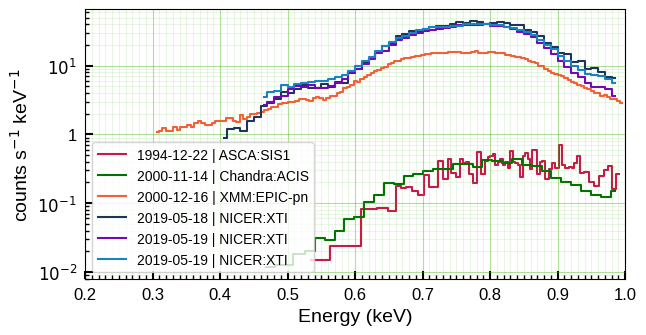
\includegraphics[width=0.8\textwidth]{images/ldata/mr-vel-counts_all-obs.png}
		        \caption{Comparison of flux from all observations from their count rates plotted to scale}
		        \label{fig:all-counts:unnorm}
    		\end{figure}
			
			\begin{figure}
				\centering
		        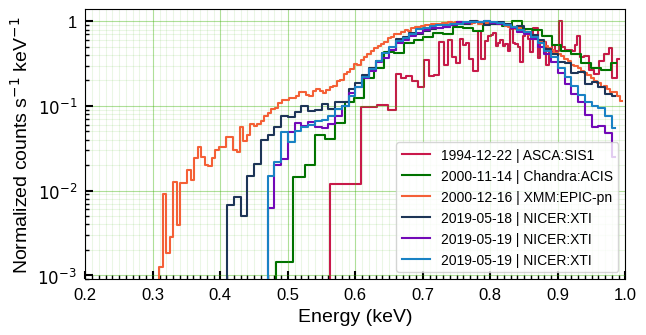
\includegraphics[width=0.8\textwidth]{images/ldata/mr-vel-normcounts_all-obs.png}
		        \caption{Normalized count rates from all observations show varying responses to supersoft X-rays}
		        \label{fig:all-counts:norm}
		    \end{figure}
		    
		    Concurrently, in figure \ref{fig:all-counts:norm}, the count rates are normalized to the range of 0 to 1 using \textit{min-max normalization}. This visualization accentuates the relative sensitivity of more recent observations to supersoft X-ray photons emitted by \source. The sub-plot shows that in recent observations the supersoft X-ray features are discernibly enhanced. This might be suggestive of improved observational capabilities or heightened sensitivity to the emitted X-ray flux.
		    
		    Together, these visualizations offer a nuanced understanding of the flux variability and observational sensitivity trends exhibited by \source\ across different observation epochs, contributing to the broader understanding of its X-ray emission characteristics.
    	
    	\subsection{NLTE Continuum Model} \label{multi-obs:results:nlte}
    		In table \ref{tab:res-fitting}, we present the luminosity, effective temperature and column density for \source\ which are derived after performing the fitting to the NLTE continuum model described in \S \ref{multi-obs:red-analysis} We also present the model fit statistics, namely the reduced $\chi^2$ values for each fit. It can be noticed that the same continuum model has been able to provide a good fit to all of the observations in our chosen dataset.
    		
    		\begin{landscape}
    		\renewcommand{\arraystretch}{2.2}
    		\begin{table}[!htb]
		    	\centering
		    	\caption{Parameters of \source\ derived from continuum NLTE model from multi-observatory observations.}
		    	\label{tab:res-fitting}
		    	\begin{tabular}{ccccccc}
					\hline
					{\textbf{Observatory}} & {\textbf{Obs. ID}} & {$\boldsymbol{L_*}$ \textbf{(erg s$\boldsymbol{^{-1}}$)}} & {\textbf{$\boldsymbol{T_\text{eff}}$ (kK)}} & {\textbf{$\boldsymbol{n_H}$ ($\boldsymbol{\times 10^{22}}$ cm$\boldsymbol{^{-2}}$)}} & {$\boldsymbol{\chi^2}$/\textbf{d.o.f}} & {$\boldsymbol{\chi^2_\text{reduced}}$} \\
					\hline
					{ASCA} & {43036000} & {$2.07_{0.46}^{71.02}\times 10^{41}$} & {$100.2_{56.2}^{147.4}$} & {$0.13_{0.00}^{1.36}$} & {75.4/62} & {1.22} \\ %updated
					{Chandra} & {644} & {$4.38_{2.02}^{24.34}\times 10^{41}$} & {$96.3_{81.6}^{120.5}$} & {$1.25_{1.17}^{1.37}$} & {30.5/28} & {1.09} \\ %updated
					{XMM-Newton} & {0111150101} & {$2.19_{1.96}^{3.74}\times 10^{42}$} & {$91.7_{86.9}^{100.2}$} & {$1.17_{1.09}^{1.27}$} & {183.4/131} & {1.40} \\ %updated
					{NICER} & {2611020101} & {$8.40_{6.77}^{19.16}\times 10^{41}$} & {$100.8_{90.0}^{110.1}$} & {$1.22_{1.11}^{1.28}$} & {65.4/52} & {1.26} \\ %updated
					{NICER} & {2611020102} & {$1.68_{1.41}^{3.37}\times 10^{41}$} & {$107.9_{100.4}^{113.8}$} & {$0.46_{0.43}^{0.54}$} & {82.9/46} & {1.80} \\ %updated
					{NICER} & {2611020103} & {$4.41_{3.42}^{6.81}\times 10^{40}$} & {$106.9_{101.6}^{110.4}$} & {$0.36_{0.34}^{0.41}$} & {83.3/46} & {1.81} \\ %updated
					\hline
				\end{tabular}
			\end{table}
			\renewcommand{\arraystretch}{1.6}
			\end{landscape}
    	
    	\subsection{Unfolded Spectra} \label{multi-obs:results:unfolded}
    		In figures \ref{fig:all-uf:12-24} and \ref{fig:all-uf:24-36}, the unfolded spectrum, which is obtained after fitting the data to the best-fit model, is displayed. The observations reveal features which are indicative of the presence of elemental absorption edges.
    		
    		\begin{figure}[!htb]
		        \centering
		        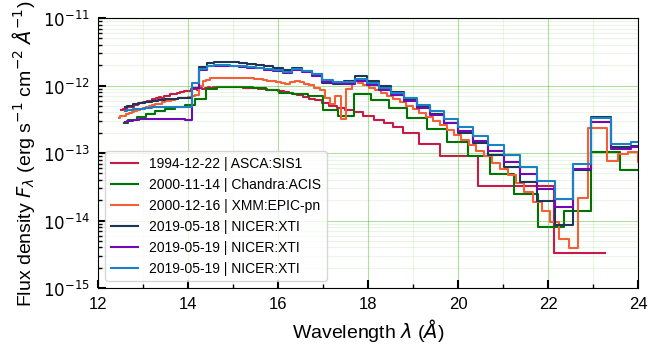
\includegraphics[width=0.8\textwidth]{images/eufspec/mr-vel-uf_all-obs_12-24.png}
		        \caption{Unfolded spectra after model fitting in the range 12 \AA - 24 \AA}
		        \label{fig:all-uf:12-24}
		    \end{figure}

		    \begin{figure}[!htb]
		    	\centering
		    	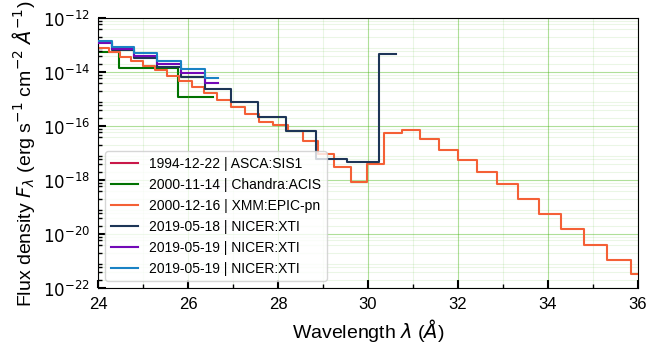
\includegraphics[width=0.8\textwidth]{images/eufspec/mr-vel-uf_all-obs_24-36.png}
		    	\caption{Unfolded spectra after model fitting in the range 24 \AA - 36 \AA}
		    	\label{fig:all-uf:24-36}
		    \end{figure}
    	
    	\subsection{Luminosity versus Effective Temperature} \label{multi-obs:results:L-vs-Teff}
    		In figure \ref{fig:L-Teff}, we present a visualization of the calculated values of the luminosity $L_*$ and effective temperature $T_\text{eff}$ for \source\ using the best-fit model. One may note that the horizontal axis, containing the $T_\text{eff}$ data is plotted as increasing from right to left, \textit{\`{a} la} Hertzsprung-Russell diagram. This enables one to compare the overlap of the regions of uncertainty of these parameters as calculated using the data from multiple observatories.
    		
    		\begin{figure}[!thb]
		    	\centering
		    	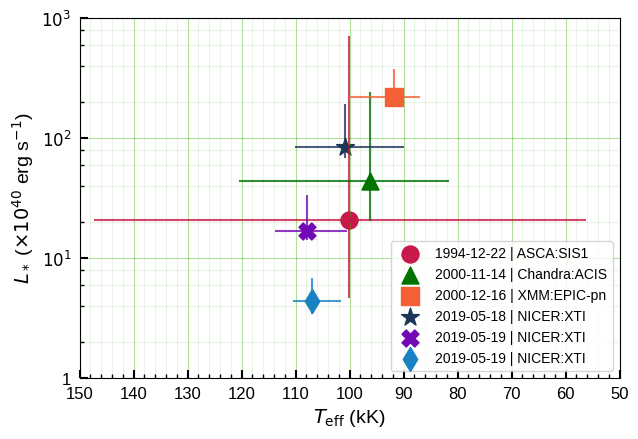
\includegraphics[width=0.9\textwidth]{images/L-Teff_all-obs.png}
		    	\caption{Uncertainties in $L_*$ and $T_\text{eff}$ calculations from multi-observatory observations of \source}
		    	\label{fig:L-Teff}
		    \end{figure}
    	
    	\subsection{Presence of Elemental Absorption Edges} \label{multi-obs:results:abs-edge}
    		During the preliminary fitting of the observations, the detection of residuals in absorption at energies of 0.402 keV, 0.532 keV, 0.708 keV and 0.867 keV suggested the presence of absorption edges. Consequently, by including relevant model components, four elemental absorption edges were detected from the best fitting model on all the observations. These absorption edges, belonging to N, O, Ne and Fe, are overlaid on the unfolded spectra and displayed in figure \ref{fig:all-uf:abs-edges}. The energies of the absorption edges were kept frozen during the fitting for all the observations.
    		
    		\begin{figure}[!htb]
		        \centering
		        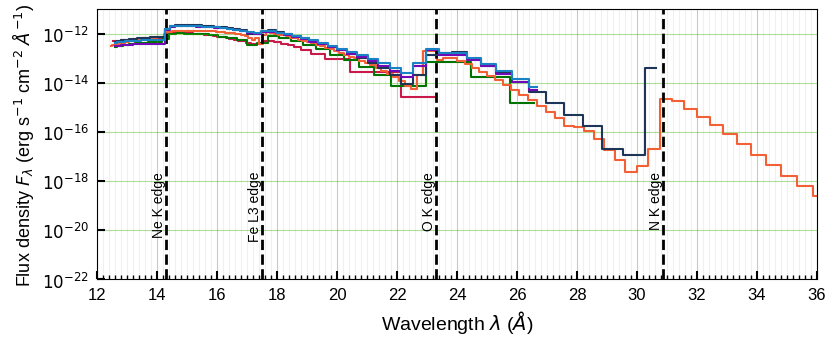
\includegraphics[width=\textwidth]{images/eufspec/mr-vel-uf-ang_abs-edge.png}
		        \caption{Unfolded spectra with overlaid elemental absorption edges}
		        \label{fig:all-uf:abs-edges}
		    \end{figure}
		    
		    \begin{landscape}
		    \renewcommand{\arraystretch}{2.2}
		    \begin{table}[!htb]
		    	\centering
		    	\caption{Absorption depth $D$ of \source\ derived from identified absorption edges of Ne, Fe, O and N.}
		    	\label{tab:abs-depth}
				\begin{tabular}{ccccccc}
					\hline
					\multirow{3}{*}{\textbf{Observatory}} & \multirow{3}{*}{\textbf{Obs. ID}} & \multicolumn{4}{c}{\textbf{Absorption Depth $\boldsymbol{D}$}} & \multirow{3}{*}{\textbf{Relative Depth}} \\ \cline{3-6} & & \textbf{Ne $\boldsymbol{K}$ edge} & \textbf{Fe $\boldsymbol{L_3}$ edge} & \textbf{O $\boldsymbol{K}$ edge} & \textbf{N $\boldsymbol{K}$ edge} \\ \cline{3-6} & & \textbf{14.302 \AA} & \textbf{17.509 \AA} & \textbf{23.305 \AA} & \textbf{30.873 \AA} \\
					\hline
					{ASCA} & {43036000} & {0.503} & {0.661} & {0.941} & {1.787} & {0.28 : 0.37 : 0.53 : 1.0} \\ %updated
					{Chandra} & {644} & {0.497} & {0.673} & {1.823} & {5.171} & {0.10 : 0.13 : 0.35 : 1.0} \\ %updated
					{XMM-Newton} & {0111150101} & {0.211} & {0.033} & {0.132} & {5.215} & {0.04 : 0.01 : 0.03 : 1.0} \\ %updated
					{NICER} & {2611020101} & {0.819} & {0.013} & {1.630} & {0.185} & {0.50 : 0.01 : 1.0 : 0.11} \\ %updated
					{NICER} & {2611020102} & {1.612} & {0.180} & {0.395} & {1.752} & {0.92 : 0.10 : 0.23 : 1.0} \\ %updated
					{NICER} & {2611020103} & {1.271} & {0.315} & {0.132} & {0.006} & {1.0 : 0.25 : 0.10 : 0.01} \\ %updated
					\hline
				\end{tabular}
			\end{table}
			\renewcommand{\arraystretch}{1.6}
		    \end{landscape}
		    
		    Because the best-fitted spectrum obtained from the EPIC-pn instrument of XMM-Newton spans the widest range of wavelengths, known absorption edges \cite{bearden1967reevaluation,juett2006high} were identified in the vicinity of the absorption edges in figure \ref{fig:all-uf:abs-edges}. These are reported in table \ref{tab:abs-depth}. Then they were overlaid on the unfolded spectrum obtained from the EPIC-pn observation. The four absorption edges that could be identified are the $K$ edges of N, O and Ne and the $L_3$ edge of Fe at 30.873 \AA, 23.305 \AA, 14.302 \AA\ and 17.509 \AA\ respectively, as displayed in the sub-plots of figure \ref{fig:pn-uf:abs-edges}. Three among these four edges, namely the $K$ edges of O and Ne and the $L_3$ edge of Fe, were reported to be present in the spectrum of \source\ using the CLOUDY photoionization code by Prodhani and Baruah (2018) \cite{prodhani2018galactic}.
		    
		    \begin{figure}[h!]
				\centering				
				\subfloat[Ne K absorption edge at 14.302 \AA \label{fig:pn-uf:Ne-edges}]{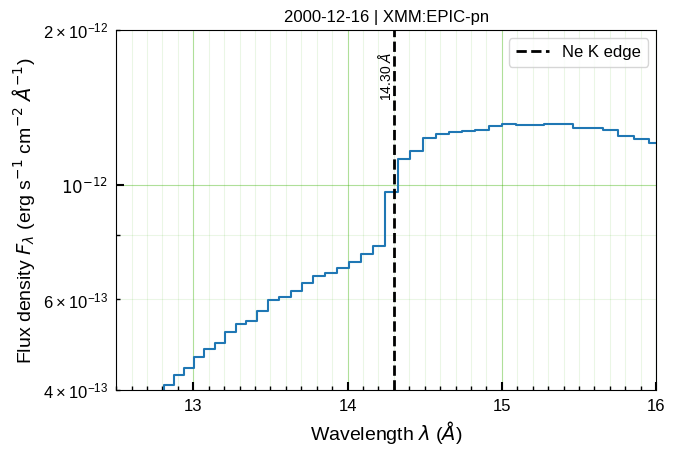
\includegraphics[width=0.5\textwidth]{images/eufspec/mr-vel-XMM-EPIC-pn-uf-Ne-edges.png}} %\hfill				
				\subfloat[Fe L$_3$ absorption edge at 17.509 \AA \label{fig:pn-uf:Fe-edges}]{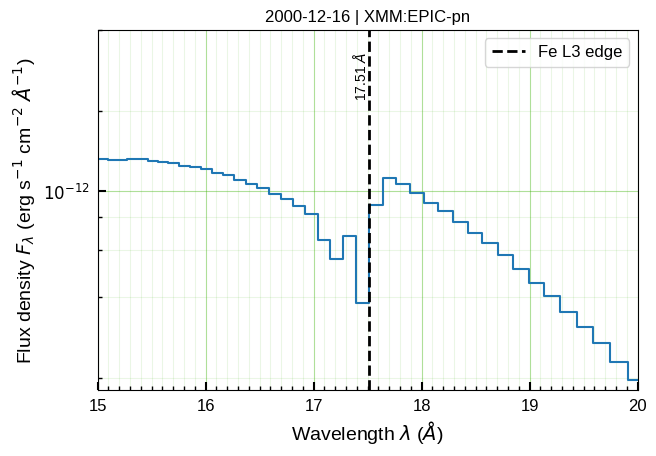
\includegraphics[width=0.5\textwidth]{images/eufspec/mr-vel-XMM-EPIC-pn-uf-Fe-edges.png}} %\hfill
				
				\subfloat[O K absorption edge at 23.305 \AA \label{fig:pn-uf:O-edges}]{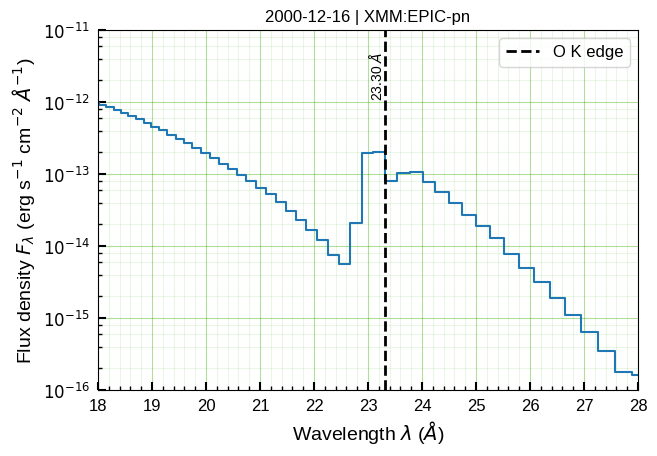
\includegraphics[width=0.5\textwidth]{images/eufspec/mr-vel-XMM-EPIC-pn-uf-O-edges.png}} %\hfill				
				\subfloat[N K absorption edge at 30.873 \AA \label{fig:pn-uf:N-edges}]{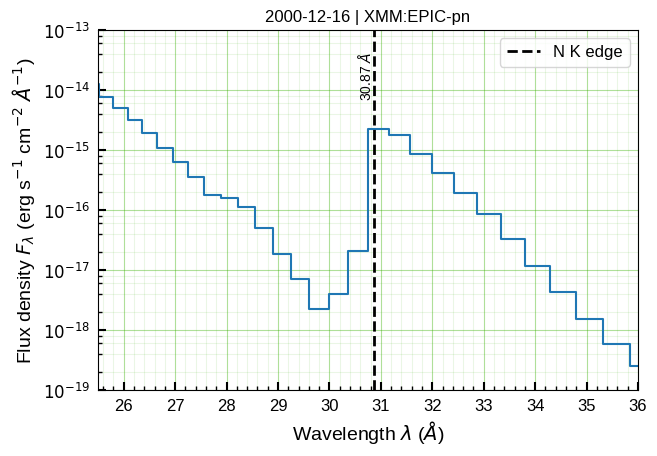
\includegraphics[width=0.5\textwidth]{images/eufspec/mr-vel-XMM-EPIC-pn-uf-N-edges.png}} %\hfill				
				\caption{Absorption edges for N, O, Ne and Fe overlaid on the unfolded spectrum for EPIC-pn observation}
		        \label{fig:pn-uf:abs-edges}
			\end{figure}

    	
    \section{Discussion} \label{multi-obs:discussion}
    	As per current literature on spectral fitting of the SSS \source, Bearda et al. (2002) and Motch et al. (2002) had arrived at the conclusion that its spectra cannot be reproduced by NLTE model atmospheres \cite{beardaChandra2002AA,motchXmmNewton2002AA}. Earlier, Hartmann et al. (1999) had applied non-local thermodynamic equilibrium (NLTE) models, which included metal line opacities, to the spectrum extracted from the observations by BeppoSAX LECS of \source\ on 25--26 January 1997 \cite{hartmann1999constraining}, where the best fit was using a model consisting of two spectral components. But nevertheless, they obtained a reduced $\chi^2>2$. In the absence of a proper model describing the emission spectrum, it becomes impossible to
derive fundamental parameters such as temperature, neutral hydrogen column density and luminosity \cite{motchXmmNewton2002AA}. Hence, obtaining an acceptable fit for \source\ spectrum assumes crucial importance at this juncture.
    
    	\subsection{Best-fit Continuum Model} \label{multi-obs:discussion:cont-mod}
    		The model, chosen for fitting the data from six different observations, consists of a publicly available\footnote{\url{http://astro.uni-tuebingen.de/~rauch/TMAF/TMAF.html}} NLTE (non-local thermal equilibrium) table model component computed from a grid of stellar model atmosphere fluxes for source emission, a photoelectric absorption model component\footnote{\url{https://heasarc.gsfc.nasa.gov/xanadu/xspec/manual/XSmodelPhabs.html}}, a model component for absorption by inter-stellar medium\footnote{\url{https://heasarc.gsfc.nasa.gov/xanadu/xspec/manual/node255.html}} and four model components to account for the presence of absorption edges\footnote{\url{https://heasarc.gsfc.nasa.gov/xanadu/xspec/manual/node247.html}}.
    		
    		Figure \ref{fig:all-obs:resid-stats} presents the residual statistics from best-fit model to all observations. The values of the fit statistic used, i.e. the reduced $\chi^2$, were all within the acceptable range of $1<\chi^2_\text{reduced}<2$, which warrants a model to be considered a good fit for the observed data. An inspection of the distribution of the residual suggests an approximately normal distribution, which can be observed in the best-fit models for all the observations, further supporting the validity of the model fit. Such a distribution of the residuals is displayed in figure \ref{fig:pn:resid-hist} for the observations of the EPIC-pn data.
    		
    		\begin{figure}[h!]
				\centering				
				\subfloat[Residuals between data and best-fit model for EPIC-pn observations \label{fig:pn:resid}]{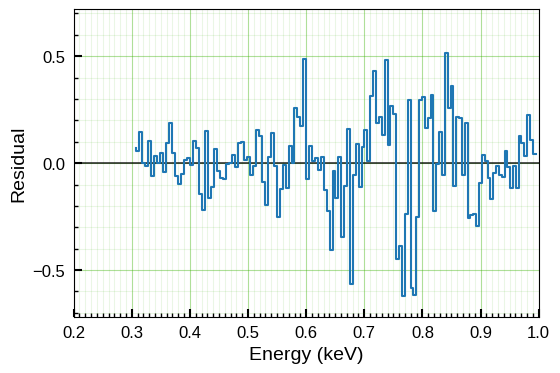
\includegraphics[width=0.48\textwidth]{images/resid/mr-vel-0111150101-pn_resid.png}} \hfill				
				\subfloat[Distribution of residuals from the best-fit model to EPIC-pn observations, along with the KDE function and fitted Gaussian \label{fig:pn:resid-hist}]{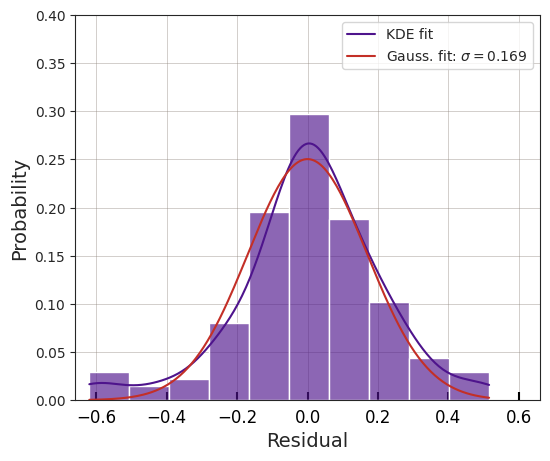
\includegraphics[width=0.48\textwidth]{images/resid/mr-vel-0111150101-pn_resid-hist.png}} %\hfill		
				\caption{Residual statistics from best-fit model to all observations}
		        \label{fig:all-obs:resid-stats}
			\end{figure}
			
			As it can be seen in figure \ref{fig:pn:resid-hist}, the kernel density estimate (KDE) function of the distribution closely approximates a normal distribution centred about zero (with zero indicating a perfect fit) and with a standard deviation of 0.169, thereby indicating that the observed count rate data can be considered to be random fluctuations which are normally distributed about the best-fit model. Therefore, the normal distribution of the residuals indicates that they are random and do not have a systematic bias (as is expected of a good fit), thereby further validating that the model fitting performed is satisfactory for all six cases of the observations.
			
			\begin{figure}[!htb]
		    	\centering
		    	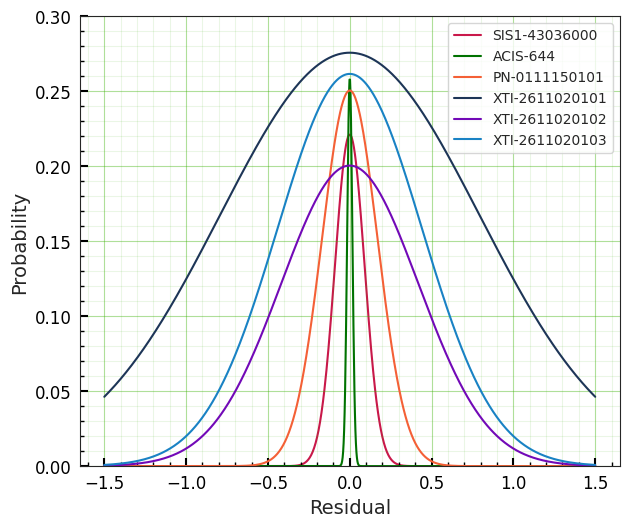
\includegraphics[width=0.8\textwidth]{images/resid/mr-vel-resid-gaussfit_all-obs.png}
		    	\caption{Gaussian approximations of the KDE functions for residual distributions of all observations}
		    	\label{fig:all-obs:resid-gaussfit}
		    \end{figure}
		    
		    In figure \ref{fig:all-obs:resid-gaussfit}, we find the Gaussian distribution fitted to all the observations. This figure shows that the quality of the fit is the best for the earlier Chandra, XMM-Newton and ASCA observations. For the recent NICER observations, the residuals show a wider spread spread about the perfect fit.
    	
    	\subsection{NLTE Pure H Model Atmosphere} \label{multi-obs:discussion:nlte-pureH}
    		In a classical stellar atmosphere, which is a plane-parallel, horizontally homogenous atmosphere in hydrostatic and radiative equilibrium, a non-LTE (or NLTE) description refers to a scenario where the energy levels of some selected species may be allowed to depart from their local thermodynamic equilibrium (LTE) values \cite{hubeny2014theory}.
    	
    		\subsubsection{Structural Equations}
    			Given below are the structural equations that are used to model an NLTE atmosphere.
    			
    			In its second-order form, the \textit{radiative transfer equation} is
    			\begin{align}
					\npdvt{2}{(f_\nu J_\nu)}{\tau_\nu}=J_\nu-S_\nu \label{eqn:rte-2nd-order}
				\end{align}
				where $J_\nu$ is the \textit{mean intensity} over all solid angles, $\tau_\nu$ the monochromatic \textit{optical depth}, $f_\nu$ the variable \textit{Eddington factor} and $S_\nu$ the \textit{source function}. The upper and lower boundary conditions on equation (\ref{eqn:rte-2nd-order}) are respectively
				\begin{align}
					&\left[ \pdvt{(f_\nu J_\nu)}{\tau_\nu} \right]_0=g_\nu J_\nu(0)-H_\nu^\text{ext} \label{eqn:rte-upper-bc} \\
					&\left[ \pdvt{(f_\nu J_\nu)}{\tau_\nu} \right]_{\tau_\text{max}}=H_\nu^+-\dfrac{1}{2}J_\nu \label{eqn:rte-lower-bc}
				\end{align}
				where $g_\nu$ is the \textit{surface Eddington factor}, $H_\nu^\text{ext}$, $H_\nu^+$ being the \textit{first angular moment} of specific intensity taken at the respective upper and lower boundaries of the current stellar atmospheric layer.
				
				The \textit{hydrostatic equilibrium equation} is re-cast as
				\begin{align}
					\dvt{P_\text{gas}}{m}=g-\dfrac{4\pi}{c}\integ{0}{\infty}{\dvt{K_\nu}{m}}{\nu}=g-\dfrac{4\pi}{c}\integ{0}{\infty}{\dfrac{\chi_\nu}{\rho}H_\nu}{\nu} \label{eqn:hyd-equil}
				\end{align}
				where $K_\nu$ is the \textit{second angular moment} of specific intensity, $\chi_\nu$ is the \textit{absorption coefficient} and $m$ is the \textit{Lagrangian mass}. In equation (\ref{eqn:hyd-equil}), the total pressure is composed of three parts: the \textit{gas pressure} $P_\text{gas}$, the \textit{radiation pressure} represented by the integrals on the right-hand side and the \textit{microturbulent pressure} $P_\text{turb}$ being ignored.
				
				The \textit{radiative equilibrium equation} is an expression of the conservation of total radiant flux. It may be written in an \textit{integral form} -- more accurate at upper atmospheric layer, or in a \textit{differential form} -- more accurate in deeper layers. To improve the accuracy, numerical algorithms implement a linear combination of both form as
				\begin{align}
					\alpha&\left[ \integ{0}{\infty}{(\kappa_\nu J_\nu-\eta_\nu)}{\nu} \right] \nonumber\\
						&+\beta\left[ \integ{0}{\infty}{\dvt{(f_\nu J_\nu)}{\tau_\nu}}{\nu}-\dfrac{\sigma_R}{4\pi}T_\text{eff}^4 \right]=0 \label{eqn:rad-equil}
				\end{align}
				where $\sigma_R$ is the Stefan-Boltzmann constant, $\kappa_\nu$, $\eta_\nu$ are the thermal absorption and emission coefficients respectively. In equation (\ref{eqn:rad-equil}) above, the term within the first pair of brackets contains the integral form and that within the second pair contains the differential form. The empirical coefficients $\alpha$, $\beta$ enable a transition from upper layers ($\alpha\rightarrow 1$, $\beta\rightarrow 0$) to lower layers ($\alpha\rightarrow 0$, $\beta\rightarrow 1$) -- such a transition is taken to be around the depth where the Rosseland mean optical depth is $\sim 1$.
				
				The \textit{kinetic equilibrium equations} (or \textit{rate equations}) are written for each chemical species, after having first selected those species which are to be considered to deviate from LTE. For any species, these equations may be represented by a matrix equation as
				\begin{align}
					\vsmat{A}\cdot\vsvec{n}=\vsvec{b} \label{eqn:kin-equil}
				\end{align}
				where the elements of the \textit{rate matrix} $\vsmat{A}$ are given as
				\begin{align*}
					\vmelem{A}{i}{j}&=\sum_{j\neq i}{(R_{ij}+C_{ij})} \\
					\vmelem{A}{i}{j}&=-(R_{ji}+C_{ji}),\text{ for }j\neq i\text{ and }i\neq k \\
					\vmelem{A}{k}{j}&=1+S_j
				\end{align*}
				with $k$ being the index of the \textit{characteristic level} and $R_{ij}$, $C_{ij}$ the radiative and collisional rates respectively between transition levels $i$ and $j$. It must be noted that $R_{ij}$'s implicitly involve the \textit{Saha-Boltzmann factor} $\Phi_i(T)$ which comes into play for \textit{bound-free transitions}, i.e. absorption edges
				\begin{align}
					\Phi_i(T)=\dfrac{g_i}{2g_1^+}\left( \dfrac{h^2}{2\pi m_e kT} \right)^{3/2}e^{(E_I-E_i)/kT} \label{eqn:saha-boltz-factor}
				\end{align}
				where $E_I$ is the ionization potential of the ion to which level $i$ belongs, $E_i$ the excitation energy of level $i$ and $g_1^+$ the statistical weight of the ground state of the next ion and $m_e$ the electronic mass. In equation (\ref{eqn:kin-equil}), $\vsvec{n}$ is the vector of populations of levels and the vector $\vsvec{b}$ has a single non-zero element corresponding to the characteristic level $k$ as
				\begin{align*}
					\vvelem{b}{i}=(N-n_e)\alpha_I\delta_{ki}
				\end{align*}
				where $N$ is the net populations of all levels, $n_e$ the number density of electrons and $\alpha_I$ the fractional abundance of the species $I$.
				
				The overall electrical neutrality of the medium is expressed by the \textit{charge conservation equation} as
				\begin{align}
					\sum_i{n_iZ_i}-n_e=0 \label{eqn:ch-cons}
				\end{align}
				where $Z_i$ is the charge associated with level $i$.
				
				The \textit{mass density}, which is related to the atomic level populations, can be expressed as
				\begin{align}
					\rho=(N-n_e)\mu m_H \label{eqn:mass-dens}
				\end{align}
				where $\mu$ is the mean molecular weight and $m_H$ is the mass of the H atom. A quantity known as the \textit{fictitious massive particle density} is defined as
				\begin{align}
					n_m\equiv(N-n_e)\mu \label{eqn:fict-mass-dens}
				\end{align}
				which then enables the mass density to be simply written as $\rho=n_m m_H$.
				
				The absorption coefficient included in equation (\ref{eqn:hyd-equil}) is written as the combination
				\begin{align}
					\chi_\nu=\kappa_\nu+\kappa_\nu^\text{sc} \label{eqn:abs-coeff}
				\end{align}
				where $\kappa_\nu$ is also known as the \textit{extinction coefficient} and $\kappa_\nu^\text{sc}$ the \textit{scattering coefficient}. The extinction coefficient is given as
				\begin{align}
					\kappa_\nu=\sum_{i}&\sum_{j>i}{[n_i-n_jG_{ij}(\nu)]\sigma_{ij}(\nu)} \nonumber\\
									&+\sum_{l}{n_en_l\sigma_{ll}(\nu,T)\left( 1-e^{-h\nu/kT} \right)}+\kappa_\nu^\text{addl} \label{eqn:ext-abs-coeff}
				\end{align}
				where the first term represents the contribution from \textit{bound-bound transitions} (i.e. absorption lines), the second represents that from \textit{bound-free transitions} (i.e. absorption edges) and the last term lumps together any additional opacity not written as detailed transitions. Here $G_{ij}=\frac{w_ig_i}{w_jg_j}$, with $g_i,g_j$ and $w_i,w_j$ being the respective degeneracies and statistical weights of levels $i$ and $j$ respectively. Also $\sigma_{ij}$ is the opacity of the transition between levels $i$ and $j$.
				
				The scattering coefficient in equation (\ref{eqn:abs-coeff}) is given as
				\begin{align}
					\kappa_\nu^\text{sc}=n_e\sigma_e + \sum_i{n_{\text{Ray},i}\sigma_{\text{Ray},i}} \label{eqn:sca-abs-coeff}
				\end{align}
				where $\sigma_e$, $\sigma_{\text{Ray},i}$ are the Thomson and Rayleigh scattering cross-sections respectively. For pure-hydrogen atmospheres with high temperatures, the Rayleigh scattering is negligible because the hydrogen atoms are expected to be fully ionized.
				
				In a similar manner, the \textit{total emission coefficient} is also expressed as a sum of thermal and scattering contributions as
				\begin{align}
					\eta_\nu^\text{total}=\eta_\nu+\eta_\nu^\text{sc} \label{eqn:em-coeff}
				\end{align}
				where
				\begin{align}
					\eta_\nu=\left(\dfrac{2h\nu^3}{c^2}\right)&\left[ \sum_{i}\sum_{j>i}{n_jG_{ij}(\nu)\sigma_{ij}(\nu)} \right. \nonumber\\
									&\left.+\sum_{l}{n_en_l\sigma_{ll}(\nu,T)e^{-h\nu/kT}}\right]+\eta_\nu^\text{addl} \label{eqn:ext-em-coeff}
				\end{align}
				in which, again, any additional emissivity is lumped together and given using the Planck function as $\eta_\nu^\text{addl}=\kappa_\nu^\text{addl}B_\nu$.
				
				Finally, taking into account the \textit{convective flux} $F_\text{conv}$ (if any) within the differential form of the radiative equilibrium equation (\ref{eqn:rad-equil}) as
				\begin{align}
					\integ{0}{\infty}{\dvt{(f_\nu J_\nu)}{\tau_\nu}}{\nu}+\dfrac{F_\text{conv}}{4\pi}=\dfrac{\sigma_R}{4\pi}T_\text{eff}^4 \label{eqn:rad-equil-2}
				\end{align}
				Differentiating equation (\ref{eqn:rad-equil-2}) with respect to the Lagrangian mass $m$ finally gives the \textit{radiative+convective equilibrium equation} as
				\begin{align}
					\integ{0}{\infty}{(\kappa_\nu J_\nu-\eta_\nu)}{\nu}+\dfrac{\rho}{4\pi}\dvt{F_\text{conv}}{m}=0 \label{eqn:rad-conv-equil}
				\end{align}
    		
    		\subsubsection{Numerical Solution using ALI}
    			Accelerated lambda iteration (ALI) is a technique used to numerically solve the radiative transfer problem, particularly in the context of stellar atmosphere modeling \cite{hubeny2003accelerated}. It accelerates the computational process by introducing a correction term that takes into account the influence of previous iterations. A simplified procedural overview of this scheme is as follows:
				\begin{enumerate}
					\item \textit{Initial guess}: Start with an initial guess for the specific intensity of radiation at different frequencies within the atmosphere. \label{step:ali-init-guess}
					\item \textit{Lambda iteration}: Calculate how the radiation interacts with the atmosphere using the current guess for intensity, considering the absorption and emission by the species in the atmosphere. \label{step:ali-lmda-itr}
					\item \textit{Correction term}: Instead of simply accepting the result from step \ref{step:ali-lmda-itr}, ALI calculates a correction term based on the difference between the current guess and the result. \label{step:ali-corr-term}
					\item \textit{Update guess}: Add this correction term to the initial guess to obtain a new estimate for the intensity. \label{step:ali-update-guess}
					\item \textit{Iterate}: Repeat steps \ref{step:ali-lmda-itr}--\ref{step:ali-update-guess} until the solution converges, meaning the intensity values no longer change significantly between iterations. \label{step:ali-iterate}
				\end{enumerate}
				
				In order to numerically solve the structural equations for NLTE, they are first discretized over all three continuous variables: optical depth $\tau$, frequency $\nu$ and angle $\theta$. These discretized structural equations, together with a number of auxiliary relations, form a system of highly coupled, non-linear equations. Then the \textit{complete linearization scheme} \cite{auer1970non} is used to treat all equations on the same footing, thus solving all structural equations simultaneously. The T\"{u}bingen NLTE Model Atmosphere Package (TMAP)\footnote{\url{http://astro.uni-tuebingen.de/~rauch/TMAP/TMAP.html}} code uses ALI to calculate the stellar atmosphere by taking into account metal line-blanketing. With an extended grid of such atmospheres of pure-hydrogen models, synthetic spectral were calculated and these are eventually used as table models in XSPEC in the present work to simulate the source emission.
    	
    	\subsection{Inferences from Results} \label{multi-obs:discussion:inference}
    		Here we are trying to understand the supersoft spectrum of \source, across observations from 1994 to 2019. The idea is to develop a robust model that explains its supersoft spectrum over different time scales and different observing instruments. The best-fit model consists of XSPEC model components which consider various factors affecting the observed spectrum:
		    \begin{enumerate}[a)]
		   		\item \texttt{atable\{}pure-H NLTE with $\log{g}=7$\texttt{\}}: for the actual radiation emitted by \source
		   		\item \texttt{edge}: for specific wavelengths where bound-free absorption is particularly strong, leading to absorption edges
		   		\item \texttt{phabs}: for describing the photoelectric absorption at the source itself.
		   		\item \texttt{ismabs}: for describing how light interacts with the intervening inter-stellar medium before reaching us
		   	\end{enumerate}
		   	
		   	Initially, a simple blackbody model failed to fit the spectrum. Blackbodies emit a characteristic spectrum based on temperature, and it seems this doesn't accurately represent the complex emission from \source. Then the supersoft X-ray emission of \source\ was modelled using an NLTE stellar atmosphere model \cite{werner1999classical}. Some of these are made available as tables in appropriate FITS format to be used with the XSPEC table model component \texttt{atable} \cite{rauch2003grid,rauch2010nlte}. These models, which are essentially pre-calculated grids, vary from one another in terms of the elemental abundances, the effective temperature $T_\text{eff}$ and the effective gravity $\log{g}$ (where the gravitational acceleration $g$ is expressed in cgs units). Choosing a particular FITS file fixed the specific elemental abundance and effective gravity. Then the fitting of the model to the data is performed by using the effective temperature $T_\text{eff}$ and the redshift $z$ as parameters.
    
		    During the analysis of the spectra from all six observations of \source, we found that only an NLTE model with a pure hydrogen atmosphere for which $\log{g}=7$ was able to provide a common model continuum spectrum that gave acceptable fit quality for all six observations. This model\footnote{\url{http://astro.uni-tuebingen.de/~rauch/TMAF/flux_H.html}}, developed and made publicly available by Rauch et al., has, as the core of its computational framework, the detailed representation of hydrogen atoms within stellar atmospheres. Using the TMAP,  plane-parallel, static, pure-hydrogen models were calculated, employing several simplifying assumptions to create a tractable model of the stellar atmosphere. Here, hydrogen is represented as a model atom, focussing on energy levels up to $n=14$ under NLTE conditions, neglecting the rapid depopulation of higher levels due to a compact star's strong gravity. Certain complexities like the exact treatment of light absorption are approximated for efficiency. Finally, the model only extends to a specific optical depths of
		    $$\log{\tau}=-8\dots+4$$
		    within the atmosphere where light can travel freely, and utilizes increased detail for calculations in specific wavelength range to ensure accuracy in that region. For the synthetic spectra, the line-broadening tables of Lemke (1997) were used \cite{lemke1997extended}.
		    
		    As it can be seen from table \ref{tab:res-fitting} and figure \ref{fig:L-Teff}, the effective temperature is obtained to be $\sim 10^5$ K for all six observations and luminosity is computed to be of the order of $10^{41}$ erg s$^{-1}$, which is about 3 orders of magnitude higher that what had been reported earlier \cite{hartmann1999constraining}. Such order of magnitude of $T_\text{eff}$ is also observed recently in similar fitting of CAL 83 spectrum using a pure-hydrogen NLTE model \cite{stecchini2023revisiting}. The high values of $T_\text{eff}$ and $L_*$ from a good fit using a pure-hydrogen model seem counterintuitive for an SSS, which is typically a white dwarf accreting from a companion star. This is because white dwarfs are usually much cooler, and the accreted material might not be pure hydrogen.
    
    		However, we need to take into account the currently accepted model for SSS which is the steady nuclear burning on the surface of a white dwarf. It is likely that the companion star to \source\ is a main-sequence star, thereby hydrogen-rich. Consequently, it is possible that only hydrogen-rich matter is able to accrete around the white dwarf. This matter, upon reaching the surface of the white dwarf, owing to its large gravity, undergoes steady nuclear burning. This may explain the success of the pure-hydrogen NLTE model in fitting its spectrum. It must be borne in mind that the high $T_\text{eff}$ likely characterizes the hot accretion disk surrounding the white dwarf, and not the white dwarf itself. Friction and compression may cause the accreting matter to attain the temperatures required to undergo steady nuclear burning.
    		
    		There are a couple of limitations to drawing such an inference regarding \source:
		    \begin{enumerate}[i.]
		    	\item The NLTE model assumes a static source, which might not be entirely accurate for a dynamic system like an accretion disk.
		    	\item The model assumes a pure-hydrogen composition, which might be a simplification of the actual accreting material.
		    \end{enumerate}
		    
		    Future modeling could explore relaxing some assumptions, such as including additional elements or allowing for a dynamic disk structure. One way to do so could be by utilising the high-resolution grating spectra from observatories, such as the reflection grating spectrometer (RGS) on-board XMM-Newton, to study the absorption line profiles observed in the spectrum of \source\ and analyzing the corresponding transitions can provide valuable insights into the dynamics of the accreting material.
		    
		    \begin{figure}[!htb]
		    	\centering
		    	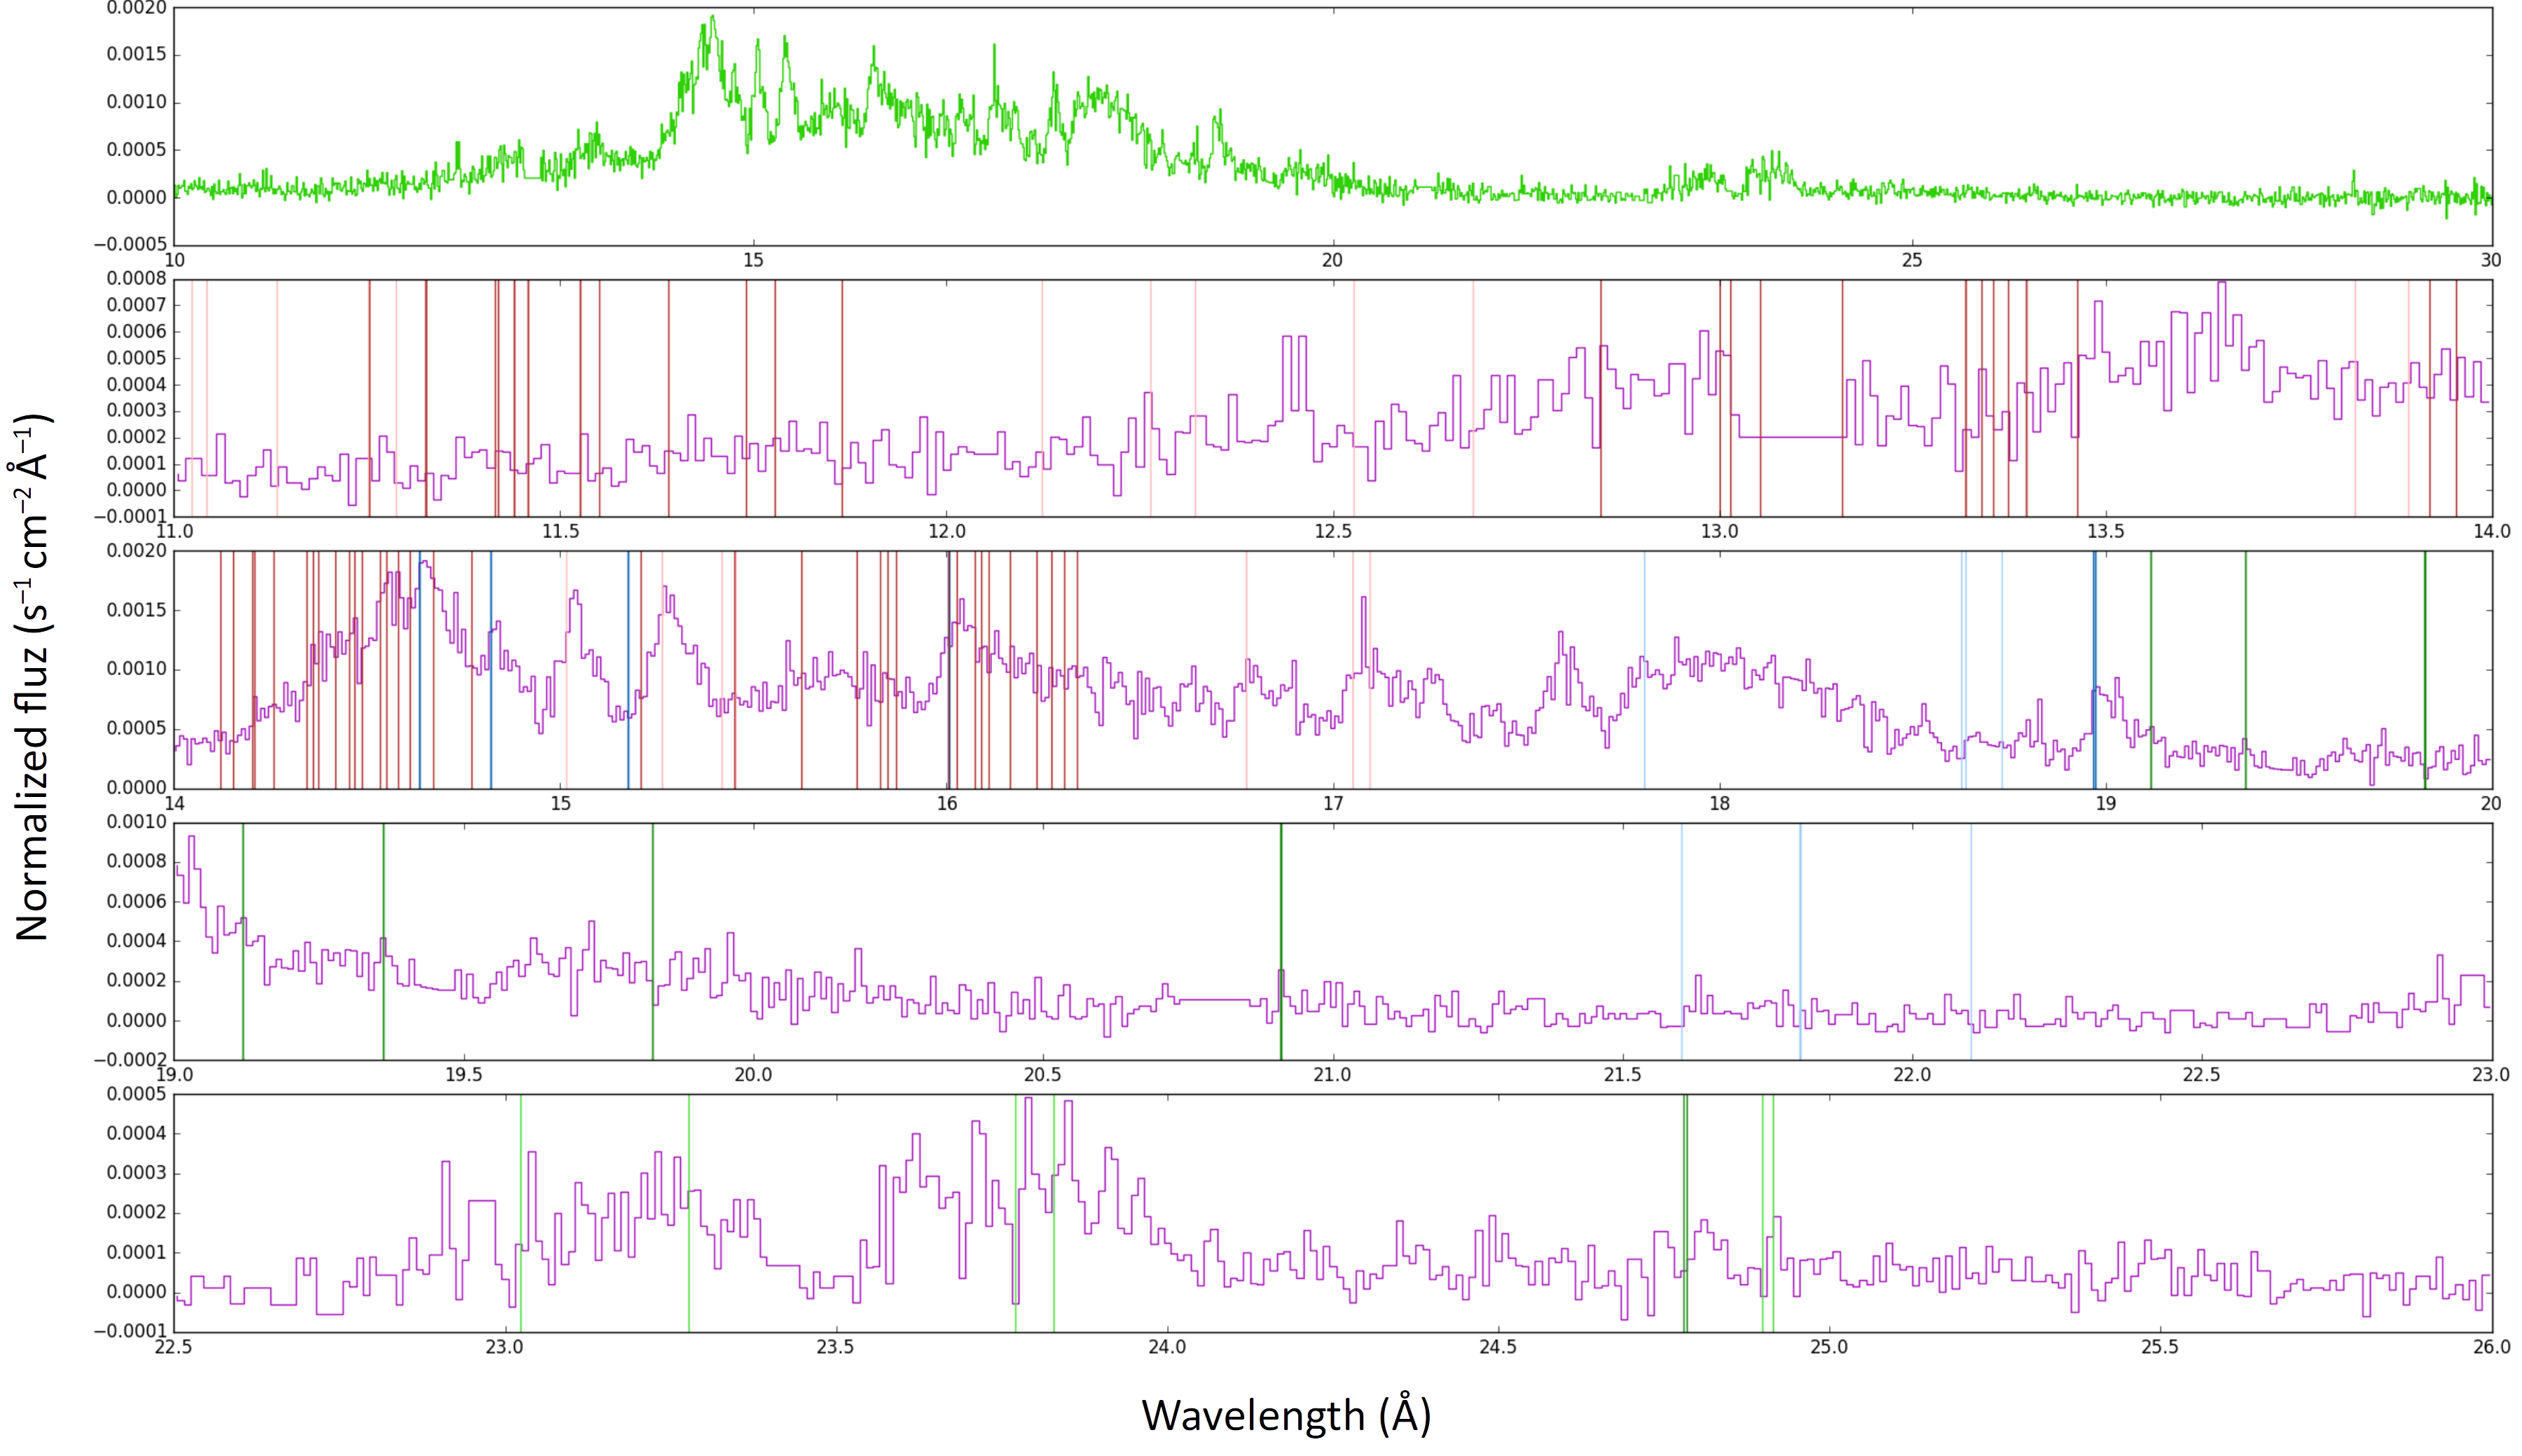
\includegraphics[width=\textwidth]{images/fig-line_identification-rgs.png}
		    	\caption{Overlay of transition lines on the fluxed RGS spectrum of \source\ for Obs. ID 0111150101. The colour scheme is: N VI and N VII lines in light and dark green respectively, O VII and O VIII lines in light and dark blue respectively, Fe XVII and Fe XVIII lines in light and dark red respectively}
		    	\label{fig:rgs-line-overlay}  
		    \end{figure}
		    
		    Absorption lines in the spectrum of \source\ arise due to the interaction of the emitted radiation with material along the line of sight. These lines exhibit diverse profiles, including shapes, widths, and shifts, which reflect the physical properties and dynamics of the absorbing material. Each absorption line corresponds to a specific transition of an atom or ion in the intervening material. Some of such lines are overlaid on the fluxed RGS spectrum of \source\ for the observation ID 0111150101, as presented in figure \ref{fig:rgs-line-overlay} \cite{bhattacharya2020python}. By identifying the atomic species and transitions associated with each absorption feature, one can gain insight into the composition and kinematics of the absorbing medium. While optical spectra have been extensively studied by categorizing them based on the presence or absence of certain spectral lines and identifying anomalies such as unusually strong or weak lines, similar approaches have been challenging to apply to X-ray spectra due to their limited spectral resolution. However, with nearly two decades of high-resolution grating spectra available from X-ray observations, it is now opportune to explore and develop methods that leverage these data to categorize and analyze X-ray spectra in more nuanced ways, such as that by Ness et al. (2013) \cite{ness2013obscuration}.
    	
    	\subsection{Relative Strengths of Absorption Edges} \label{multi-obs:discussion:abs-edge-strength}
    		Absorption edges are included in an XSPEC model using the multiplicative component named \texttt{edge}. On a continuum model, an absorption edge may be modelled as follows:
		    \begin{align}
		    	M(E)=\begin{cases}
		    		{1;\quad E\leqslant E_\text{th}} \\
		    		{\exp{\left[ -D\left(\dfrac{E}{E_\text{th}}\right)^{-3} \right]};\quad E> E_\text{th}}
		    	\end{cases} \label{eqn:edge-comp}
		    \end{align}
		    In equation (\ref{eqn:edge-comp}), $E_\text{th}$ is the \textit{threshold energy} and $D$ is the \textit{absorption depth}. The model component is implemented with these two quantities being its parameters. The relative values of the absorption depths enables a comparison of the strengths of the absorption edges.
		    
		    The absorption depths calculated from the unfolded spectra, after obtaining the best fit to the model, are presented in table \ref{tab:abs-depth}. In all six observations, the same absorption edges were identified. For the observations made by ASCA, Chandra and XMM-Newton, the identified edges show the same trend with respect to the relative strengths of the absorption depths of these edges, i.e. the N $K$ absorption edge is the strongest, followed by the O $K$ edge, the Fe $L_3$ edge and the Ne $K$ edge with similar strengths.
		    
		    However, this is not the case for the three NICER observations, each of which show different edges to be the strongest. The reasons for such an inconsistency might range from instrumental effects (such as variations in the detector response with time, or changes in the gain calibration between observations) to issues with data reduction (such as inconsistencies in background subtraction, or inaccuracies in deadtime correction). Because NICER is a relatively new mission, it is a worthwhile exercise to investigate this particular inconsistency in absorption depth strength, which would include a detailed review of the NICER calibration documents, analysis of data from different detector regions, comparison with published data on similar sources and submission of relevant science proposals for new observations.			% COMPLETE
    \chapter{FITTING THE HIGH RESOLUTION SPECTRUM OF RX J0925.7-4758 USING COMPOSITE XSPEC MODEL} \label{chap:hi-resolution}
    %\doublespacing
    \minitoc
    \begin{center}
    	\emph{Abstract of chapter \ref{chap:hi-resolution}}
    \end{center}

	\section{RGS Spectra from XMM-Newton} \label{hi-resolution:rgs-spec}
		X-ray data with high spectral resolution in the range 100 to 500 FWHM in the energy range 0.33-2.5 keV can be obtained using the RGS instruments on board the XMM-Newton satellite. In this energy range, there is a multitude of X-ray emission lines, which include the K-shell transitions and He-line triplets of light elements, such as C, N, O, Ne, Mg and Si. This energy range also includes the L-shell transitions of heavier elements such as Fe and Ni. Consequently, the RGS spectra have immense use as diagnostic tools which can be used to further investigate the high-energy physics in the emitting material \cite{xmmUserHandbook}.
		
		\begin{figure}[h!]
			\centering
			\caption{Schematic of the RGS instruments of XMM-Newton}
			\label{xmm-rgs-instrument}
			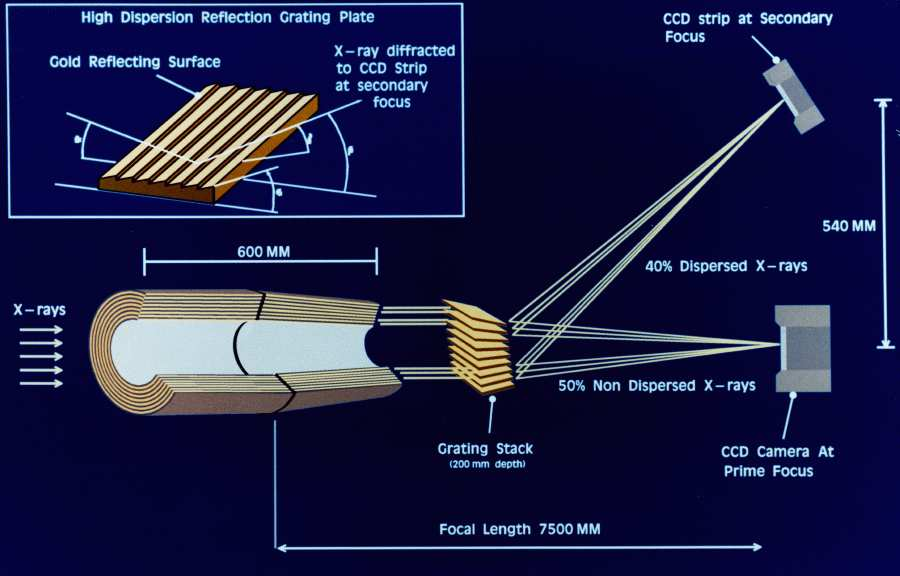
\includegraphics[width=0.9\textwidth]{xmm-rgs.png}
		\end{figure}
		
		The XMM-Newton satellite has three telescopes, out of which two are equipped with RGS instruments; these are referred to as RGS1 and RGS2. Each of these RGS instruments comprise of Reflection Grating Assemblies (RGAs) and RGS Focal Cameras (RFCs). These are referred to as \emph{grating stack} and \emph{CCD strip} in figure \ref{xmm-rgs-instrument}.
		
		The light path of the two X-ray telescopes are focussed onto the EPIC MOS cameras at the primary focus. The RGAs intercept $\sim 58\%$ of the light on the light path and diffracts it to the RFCs at the secondary focus. In order to diffract the light, the RGAs have grating plates with groove densities of $\sim 645.6$ lines mm$^{-1}$. This produces the two prominent first and second order spectra with dispersion of 8.3 and 12.7 mm \AA$^{-1}$ at 15 \AA. The performance of various parameters of the RGS instruments, while in orbit, are summarised in the table \ref{xmm-rgs-performance}.
		
		\begin{table}[h!]
			\centering
			\caption{In-orbit performance of RGS instruments}
			\label{xmm-rgs-performance}
			\begin{tabular}{|l|l|c|c|c|c|c|c|}
				\hline
				\multicolumn{2}{|l|}{\multirow{2}{*}{\textbf{Parameter}}} & \multicolumn{3}{c|}{\textbf{RGS1}} & \multicolumn{3}{c|}{\textbf{RGS2}} \\ \cline{3-8}
				\multicolumn{2}{|l|}{} & {10 \AA} & {15 \AA} & {35 \AA} & {10 \AA} & {15 \AA} & {35 \AA} \\ \hline
				\multirow{2}{*}{Effective area (cm$^2$)} & {1$^\text{st}$ order} & {51} & {61} & {21} & {53} & {68} & {25} \\ \cline{2-8}
														 & {2$^\text{nd}$ order} & {29} & {15} & {--} & {31} & {19} & {--} \\ \hline
				\multirow{2}{*}{Resolution (km s$^{-1}$)}& {1$^\text{st}$ order} & {1700} & {1200} & {600} & {1900} & {1400} & {700} \\ \cline{2-8}
														 & {2$^\text{nd}$ order} & {1000} & {700} & {--} & {1200} & {800} & {--} \\ \hline
				\multirow{2}{*}{Wavelength range} & {1$^\text{st}$ order} & \multicolumn{6}{c|}{5 -- 38 \AA (0.35 -- 2.5 keV)} \\ \cline{2-8}
												   & {2$^\text{nd}$ order} & \multicolumn{6}{c|}{5 -- 20 \AA (0.62 -- 2.5 keV)} \\ \hline
				\multirow{2}{*}{Wavelength accuracy} & {1$^\text{st}$ order} & \multicolumn{3}{c|}{$\pm$5 m\AA} & \multicolumn{3}{c|}{$\pm$5 m\AA} \\ \cline{2-8}
                                                  	  & {2$^\text{nd}$ order} & \multicolumn{3}{c|}{$\pm$4 m\AA} & \multicolumn{3}{c|}{$\pm$3 m\AA} \\ \hline
				\multicolumn{2}{|l|}{\multirow{2}{*}{Bin size {[}$3\times 3$ (27 $\mu$)$^2$ pixels{]}}} & \multicolumn{6}{c|}{2.5 arcsec (cross dispersion direction)} \\ \cline{3-8}
				\multicolumn{2}{|l|}{} & \multicolumn{6}{c|}{7 -- 14 m\AA (dispersion direction, first order)} \\ \hline
			\end{tabular}
		\end{table}
		
		The reflection grating used in the RGS instruments diffract into the first and second spectral orders with the highest efficiency -- therefore these two orders produce the most useful data. Even though the third order spectra are present, their count rates are $\sim 8$ times lower than that in the second order. Therefore, the science data provided by the XMM-Newton SOC consists of spectral data from first and second orders only. Table \ref{xmm-rgs-wavelength} summarises the wavelength range covered by the different spectral orders of the RGS instruments.
		\begin{table}[h!]
			\centering
			\caption{Wavelength ranges covered by RGS}
			\label{xmm-rgs-wavelength}
			\begin{tabular}{|c|c|}
				\hline
				{\textbf{Order}} & {\textbf{Wavelength range (\AA)}} \\
				\hline
				{1} & {6 -- 38} \\
				\hline
				{2} & {6 -- 20} \\
				\hline
			\end{tabular}
		\end{table}
	
	\section{Models for Data Fitting} \label{hi-resolution:models}
		Given below in table \ref{xmm-rgs-model-list} is the progression of Xspec models used in the analysis of the RGS spectrum of RX J0925.7-4758. Every model is given a model ID and hereinafter it will be referred to by the same. The progression of the models is evolutionary and follows the same sequence as each was built from the preceding model.
		
		For instance, the first model, i.e. M01 is a simple model which is composed of two model components -- an additive component (\texttt{bbody}) and a multiplicative component (\texttt{tbabs}). This particular model was mainly used to get started with the modelling of the continuum spectrum using a blackbody emission, subjected to absorption. Then, as one progresses downwards along table \ref{xmm-rgs-model-list}, one finds models which are improvements upon the previous model, in terms of the replacement of existing model components or the addition of newer ones.
		\begin{table}[h!]
			\centering
			\caption{List of models used for data fitting}
			\label{xmm-rgs-model-list}
			\begin{tabular}{|l|l|l|}
				\hline
				\textbf{S. No.} & \textbf{Model ID} & \textbf{Xspec model} \\ \hline
				{1} & {M01} & \texttt{tbabs*bbody} \\ \hline
				{2} & {M02} & \texttt{ismabs*bbody} \\ \hline
				{3} & {M03} & \texttt{ismabs*(gauss+bbody)} \\ \hline
				{4} & {M04} & \texttt{ismabs*edge$^3$*(gauss+bbody)} \\ \hline
				{5} & {M05} & \texttt{ismabs*edge$^3$*(mekal+bbody)} \\ \hline
				{6} & {M06} & \texttt{ismabs*(apec+mekal)*swind1} \\ \hline
				{7} & {M07} & \texttt{ismabs*(gauss+mekal+bbody)} \\ \hline
				{8} & {M08} & \texttt{ismabs*(gauss+mekal+bbody)*swind1} \\ \hline
				{9} & {M09} & \texttt{ismabs*(rauch+mekal)*swind1} \\ \hline
				{10} & {M10} & \texttt{ismabs*(rauch+apec)*swind1} \\ \hline
				{11} & {M11} & \texttt{ismabs*(rauch*tbabs+apec+mekal)*swind1} \\ \hline
				{12} & {M12} & \texttt{ismabs*(rauch+apec+mekal)*swind1} \\ \hline
			\end{tabular}
		\end{table}
	
		\subsection{Model Components} \label{hi-resolution:models:components}
		
			\subsubsection{X-ray photoabsorption model: \texttt{ismabs}}
			The \texttt{ismabs} multiplicative model in Xspec provides a way to simulate X-ray photoabsorption \cite{ismabs_gatuzz}. This model incorporates variable columns for both neutral and ionized species from H, He, N, O, Ne, Mg, Si, S, Ar, Ca, Fe, Ni and Zn.
			
			Because of an inherent degeneracy between the relative columns of H, He I, He II, the column density of He I is not included as a free parameter in the model.
			
			In this model, the absorption cross-sections for various species are sourced as follows:
			\begin{itemize}
				\item Neutral states of Si, S, Ar and Ca from Verner et al. \cite{vernerXS}
				\item Singly and doubly ionized states of Si, S, Ar and Ca from Witthoeft et al. \cite{witthoeftXS1,witthoeftXS2}
				\item Neutral, singly and doubly ionized states of N from Garcia et al. \cite{garciaXS1}
				\item Neutral states of O from Gorczyca et al. \cite{gorczycaXS1}
				\item Singly and doubly ionized states of O from Garcia et al. \cite{garciaXS2}, including corrections applied by Gatuzz et al. \cite{gatuzzXS}
				\item Neutral state of Ne from Gorczyca et al. \cite{gorczycaXS2}
				\item Singly and doubly ionized states of Ne from Gorczyca et al. \cite{gorczycaXS3}
				\item For the Fe-L edge region we use the measurement of metallic iron by Kortright \& Kim \cite{kortrightXS}
				\item Neutral, singly and doubly ionized states of Mg from Hasoglu et al. (2014).
			\end{itemize}
			
			The parameters for the \texttt{ismabs} model are given in table \ref{param:ismabs}.
			\begin{table}[h!]
				\centering
				\caption{Model parameters for \texttt{ismabs}}
				\label{param:ismabs}
				\begin{tabular}{|p{3cm}|p{10cm}|}
					\hline
					\textbf{Parameter} & \textbf{Quantity} \\ \hline
					{\texttt{par1}} & {H column (in $10^{22}$ cm$^{-2}$)} \\ \hline
					{\texttt{par2}} & {He II column (in $10^{22}$ cm$^{-2}$)} \\ \hline
					{\texttt{par3}} & {C I column (in $10^{22}$ cm$^{-2}$)} \\ \hline
					{\texttt{par4}} & {C II column (in $10^{22}$ cm$^{-2}$)} \\ \hline
					{\texttt{par5}} & {C III column (in $10^{22}$ cm$^{-2}$)} \\ \hline
					{\texttt{par6}} & {N I column (in $10^{22}$ cm$^{-2}$)} \\ \hline
					{\texttt{par7}} & {N II column (in $10^{22}$ cm$^{-2}$)} \\ \hline
					{\texttt{par8}} & {N III column (in $10^{22}$ cm$^{-2}$)} \\ \hline
					{\texttt{par9}} & {O I column (in $10^{22}$ cm$^{-2}$)} \\ \hline
					{\texttt{par10}} & {O II column (in $10^{22}$ cm$^{-2}$)} \\ \hline
					{\texttt{par11}} & {O III column (in $10^{22}$ cm$^{-2}$)} \\ \hline
					{\texttt{par12}} & {Ne I column (in $10^{22}$ cm$^{-2}$)} \\ \hline
					{\texttt{par13}} & {Ne II column (in $10^{22}$ cm$^{-2}$)} \\ \hline
					{\texttt{par14}} & {Ne III column (in $10^{22}$ cm$^{-2}$)} \\ \hline
					{\texttt{par15}} & {Mg I column (in $10^{22}$ cm$^{-2}$)} \\ \hline
					{\texttt{par16}} & {Mg II column (in $10^{22}$ cm$^{-2}$)} \\ \hline
					{\texttt{par17}} & {Mg III column (in $10^{22}$ cm$^{-2}$)} \\ \hline
					{\texttt{par18}} & {Si I column (in $10^{22}$ cm$^{-2}$)} \\ \hline
					{\texttt{par19}} & {Si II column (in $10^{22}$ cm$^{-2}$)} \\ \hline
					{\texttt{par20}} & {Si III column (in $10^{22}$ cm$^{-2}$)} \\ \hline
					{\texttt{par21}} & {S I column (in $10^{22}$ cm$^{-2}$)} \\ \hline
					{\texttt{par22}} & {S II column (in $10^{22}$ cm$^{-2}$)} \\ \hline
					{\texttt{par23}} & {S III column (in $10^{22}$ cm$^{-2}$)} \\ \hline
					{\texttt{par24}} & {Ar I column (in $10^{22}$ cm$^{-2}$)} \\ \hline
					{\texttt{par25}} & {Ar II column (in $10^{22}$ cm$^{-2}$)} \\ \hline
					{\texttt{par26}} & {Ar III column (in $10^{22}$ cm$^{-2}$)} \\ \hline
					{\texttt{par27}} & {Ca I column (in $10^{22}$ cm$^{-2}$)} \\ \hline
					{\texttt{par28}} & {Ca II column (in $10^{22}$ cm$^{-2}$)} \\ \hline
					{\texttt{par29}} & {Ca III column (in $10^{22}$ cm$^{-2}$)} \\ \hline
					{\texttt{par30}} & {Fe column (in $10^{22}$ cm$^{-2}$)} \\ \hline
					{\texttt{par31}} & {Redshift $z$} \\ \hline
				\end{tabular}
			\end{table}
			
			\subsubsection{Astrophysical plasma emission code: \texttt{apec}}
				The \texttt{apec} additive model in Xspec simulates an emission spectrum that is obtained from a collisionally-ionized diffuse gas \cite{smithAPEC}. The atomic data for collisional and radiative rates, recombination cross sections, dielectronic recombination rates, and satellite line wavelengths are taken from the Astrophysical Plasma Emission Database (APED).
			
				The \texttt{apec} model provides a way to create emission models for plasma, which can be used to analyse spectral data from high-resolution X-ray spectrometers, as in the case of XMM-Newton or Chandra. The current version of the code stores the atomic data in FITS files, thereby separating it from the code. This optimizes limitations on the speed and memory across different computers.
			
				The \texttt{apec} model simulates a hot, optically thin plasma which is in a collisional ionization equilibrium, and computes both resulting continuum and line emissivities. Here, the \textit{emissivity} of a spectral line is defined as the  total number of radiative transitions per unit volume divided by the product of the electron density $n_e$ and the hydrogen (neutrals and protons) density $n_H$ in the astrophysical plasma, resulting in line emissivities having units of cm$^3$ s$^{-1}$.
			
				The parameters for the \texttt{apec} model are given in table \ref{param:apec}.
				\begin{table}[h!]
					\centering
					\caption{Model parameters for \texttt{apec}}
					\label{param:apec}
					\begin{tabular}{|p{3cm}|p{10cm}|}
						\hline
						\textbf{Parameter} & \textbf{Quantity} \\ \hline
						{\texttt{par1}} & {Plasma temperature (in keV)} \\ \hline
						{\texttt{par2}} & {Abundances of the metals C, N, O, Ne, Mg, Al, Si, S, Ar, Ca, Fe, Ni} \\ \hline
						{\texttt{par3}} & {Redshift $z$} \\ \hline
						{\texttt{norm}} & {Normalization of the component computed as $\displaystyle\dfrac{10^{-14}}{4\pi[D_A(1+z)]^2}\int{n_en_H\diff{V}}$, where $D_A$ is the angular diameter distance to the source (in cm), $n_e$ and $n_H$ are the electron densities (in cm$^{-3}$) respectively} \\ \hline
					\end{tabular}
				\end{table}

			\subsubsection{Model for emission due to optically-thin plasma: \texttt{mekal}}
				The additive model \texttt{mekal} in Xspec allows the simulation of an emission spectrum due to a diffuse plasma, whose electrons have a Maxwellian energy distribution. This model uses the spectral line list as calculated by Mewe and Kaastra \cite{meka}, additional calculations for L-shell of Fe ions by Liedahl et al. \cite{liedahl}. The model provides the option to either calculate the spectrum by running the \texttt{mekal} code, or by interpolation on a pre-calculated \texttt{mekal} table, or simply by using the AtomDB data.
				
				The models \texttt{mekal} and \texttt{apec} both simulate emission due to optically-thin plasma, the difference being in the methodology of calculation of the line lists.
				
				The parameters for the \texttt{mekal} model are given in table \ref{param:mekal}.
				\begin{table}[h!]
					\centering
					\caption{Model parameters for \texttt{mekal}}
					\label{param:mekal}
					\begin{tabular}{|p{3cm}|p{10cm}|}
						\hline
						\textbf{Parameter} & \textbf{Quantity} \\ \hline
						{\texttt{par1}} & {Plasma temperature (in keV)} \\ \hline
						{\texttt{par2}} & {H density (in cm$^{-3}$)} \\ \hline
						{\texttt{par3}} & {Metal abundances for the elements C, N, O, Ne, Na, Mg, Al, Si, S, Ar, Ca, Fe, Ni} \\ \hline
						{\texttt{par4}} & {Redshift $z$} \\ \hline
						{\texttt{par5}} & {Switch between \texttt{mekal} calculation (0), interpolation (1) and interpolation using AtomDB data (2)} \\ \hline
						{\texttt{norm}} & {Normalization of the component computed as $\displaystyle\dfrac{10^{-14}}{4\pi[D_A(1+z)]^2}\int{n_en_H\diff{V}}$, where $D_A$ is the angular diameter distance to the source (in cm), $n_e$ and $n_H$ are the electron densities (in cm$^{-3}$) respectively} \\ \hline
					\end{tabular}
				\end{table}
			
			\subsubsection{Velocity shear absorption: \texttt{swind1}}
				Originally meant for AGN spectra, the \texttt{swind1} multiplicative model fits the soft excess in partially ionized absorbing material with a large velocity shear. This is approximated by the model component by using XSTAR kn5 photoionization absorption model grids, which were calculated assuming a micro-turbulence of 100 km/s, and subsequently convolving with Gaussian smearing \cite{swind1}.
				
				In this work, the \texttt{swind1} component is used as a proxy model for possible stellar wind from the source RX J0925.7-4758, which may be indicated by the presence of P Cygni profiles in its spectrum.
				
				The parameters for the \texttt{swind1} model are given in table \ref{param:swind1}.
				\begin{table}[h!]
					\centering
					\caption{Model parameters for \texttt{swind1}}
					\label{param:swind1}
					\begin{tabular}{|p{3cm}|p{10cm}|}
						\hline
						\textbf{Parameter} & \textbf{Quantity} \\ \hline
						{\texttt{par1}} & {Column density (in $10^{22}$ cm$^{-2}$)} \\ \hline
						{\texttt{par2}} & {$\log{\xi}$ where $\xi=L/nr^2$} \\ \hline
						{\texttt{par3}} & {$\sigma$: Gaussian $\sigma$ for velocity smearing ($v/c$)} \\ \hline
						{\texttt{par4}} & {Redshift $z$} \\ \hline
					\end{tabular}
				\end{table}
			
			\subsubsection{T\"{u}bingen NLTE Model-Atmosphere Package: \texttt{rauch}}
				The T\"{u}bingen NLTE Model-Atmosphere Package (TMAP) is a tool to calculate stellar atmospheres in spherical or plane-parallel geometry in hydrostatic and radiative equilibrium allowing departures from local thermodynamic equilibrium (LTE) for the population of atomic levels \cite{wernerDreizler}. TMAP is based on the so-called Accelerated Lambda Iteration (ALI) method and is able to account for line blanketing by metals \cite{rauchALI}. All elements from hydrogen to nickel may be included in the calculation with model atoms which are tailored for the aims of the user \cite{wernerTMAP}.
				
				The web-link to a set of theoretical spectral energy distributions (SEDs) of TMAP NLTE model atmospheres were provided by Rauch \cite{rauchFITS}, which contained a grid of 10 FITS files for varying temperatures. The abundances of various elements for this grid are given in table \ref{rauch:abundances}. The TMAP model series refer to the files corresponding to the model atmosphere grid, with each column named after the last three characters of the FITS filename. The grid is calculated for effective temperatures in the range $4.50\times 10^5\,\text{K}\leqslant T_\text{eff}\leqslant 1.05\times 10^6\,\text{K}$ in steps $\Delta T=10^4\,\text{K}$. The effective surface gravity is $\log_{10}{g}=9$. The fluxes in the SEDs are calculated using the TMAP code from models with different elemental abundance ratios $[X]$.
				
				\begin{table}[h!]
					\centering
					\caption{Elemental abundances for TMAP grid}
					\label{rauch:abundances}
					\begin{tabular}{|c|cccccccccc|}
						\hline
						\multirow{2}{*}{\textbf{{[}X{]}}} & \multicolumn{10}{c|}{\textbf{TMAP model series}} \\ \cline{2-11} & \multicolumn{1}{c|}{\textbf{003}} & \multicolumn{1}{c|}{\textbf{004}} & \multicolumn{1}{c|}{\textbf{005}} & \multicolumn{1}{c|}{\textbf{006}} & \multicolumn{1}{c|}{\textbf{007}} & \multicolumn{1}{c|}{\textbf{008}} & \multicolumn{1}{c|}{\textbf{009}} & \multicolumn{1}{c|}{\textbf{010}} & \multicolumn{1}{c|}{\textbf{011}} & \textbf{201} \\ \hline
						{[}H{]} & \multicolumn{1}{c|}{-0.688} & \multicolumn{1}{c|}{-0.683} & \multicolumn{1}{c|}{-0.677} & \multicolumn{1}{c|}{-0.673} & \multicolumn{1}{c|}{-0.672} & \multicolumn{1}{c|}{-0.671} & \multicolumn{1}{c|}{-0.670} & \multicolumn{1}{c|}{-0.670} & \multicolumn{1}{c|}{-0.669} & -0.885 \\ \hline
						{[}He{]} & \multicolumn{1}{c|}{0.382} & \multicolumn{1}{c|}{0.387} & \multicolumn{1}{c|}{0.393} & \multicolumn{1}{c|}{0.397} & \multicolumn{1}{c|}{0.398} & \multicolumn{1}{c|}{0.399} & \multicolumn{1}{c|}{0.400} & \multicolumn{1}{c|}{0.401} & \multicolumn{1}{c|}{0.401} & 0.489 \\ \hline
						{[}C{]} & \multicolumn{1}{c|}{-1.513} & \multicolumn{1}{c|}{-1.073} & \multicolumn{1}{c|}{-0.772} & \multicolumn{1}{c|}{-0.675} & \multicolumn{1}{c|}{-0.596} & \multicolumn{1}{c|}{-0.529} & \multicolumn{1}{c|}{-0.471} & \multicolumn{1}{c|}{-0.420} & \multicolumn{1}{c|}{-0.374} & -0.057 \\ \hline
						{[}N{]} & \multicolumn{1}{c|}{1.803} & \multicolumn{1}{c|}{1.678} & \multicolumn{1}{c|}{1.460} & \multicolumn{1}{c|}{1.159} & \multicolumn{1}{c|}{1.062} & \multicolumn{1}{c|}{0.937} & \multicolumn{1}{c|}{0.761} & \multicolumn{1}{c|}{0.460} & \multicolumn{1}{c|}{0.159} & 1.668 \\ \hline
						{[}O{]} & \multicolumn{1}{c|}{1.528} & \multicolumn{1}{c|}{1.533} & \multicolumn{1}{c|}{1.538} & \multicolumn{1}{c|}{1.543} & \multicolumn{1}{c|}{1.544} & \multicolumn{1}{c|}{1.544} & \multicolumn{1}{c|}{1.545} & \multicolumn{1}{c|}{1.546} & \multicolumn{1}{c|}{1.547} & 1.206 \\ \hline
						{[}Ne{]} & \multicolumn{1}{c|}{-0.474} & \multicolumn{1}{c|}{-0.469} & \multicolumn{1}{c|}{-0.464} & \multicolumn{1}{c|}{-0.459} & \multicolumn{1}{c|}{-0.459} & \multicolumn{1}{c|}{-0.458} & \multicolumn{1}{c|}{-0.457} & \multicolumn{1}{c|}{-0.456} & \multicolumn{1}{c|}{-0.456} & -0.517 \\ \hline
						{[}Mg{]} & \multicolumn{1}{c|}{-0.454} & \multicolumn{1}{c|}{-0.450} & \multicolumn{1}{c|}{-0.444} & \multicolumn{1}{c|}{-0.439} & \multicolumn{1}{c|}{-0.439} & \multicolumn{1}{c|}{-0.438} & \multicolumn{1}{c|}{-0.437} & \multicolumn{1}{c|}{-0.436} & \multicolumn{1}{c|}{-0.436} & -0.497 \\ \hline
						{[}Si{]} & \multicolumn{1}{c|}{0.167} & \multicolumn{1}{c|}{0.172} & \multicolumn{1}{c|}{0.178} & \multicolumn{1}{c|}{0.182} & \multicolumn{1}{c|}{0.183} & \multicolumn{1}{c|}{0.184} & \multicolumn{1}{c|}{0.185} & \multicolumn{1}{c|}{0.186} & \multicolumn{1}{c|}{0.186} & 0.125 \\ \hline
						{[}S{]} & \multicolumn{1}{c|}{-1.583} & \multicolumn{1}{c|}{-1.578} & \multicolumn{1}{c|}{-1.573} & \multicolumn{1}{c|}{-1.568} & \multicolumn{1}{c|}{-1.567} & \multicolumn{1}{c|}{-1.567} & \multicolumn{1}{c|}{-1.566} & \multicolumn{1}{c|}{-1.565} & \multicolumn{1}{c|}{-1.565} & -1.625 \\ \hline
						{[}IG{]} & \multicolumn{1}{c|}{0.828} & \multicolumn{1}{c|}{0.833} & \multicolumn{1}{c|}{0.838} & \multicolumn{1}{c|}{0.843} & \multicolumn{1}{c|}{0.843} & \multicolumn{1}{c|}{0.844} & \multicolumn{1}{c|}{0.845} & \multicolumn{1}{c|}{0.846} & \multicolumn{1}{c|}{0.846} & 0.786 \\ \hline
					\end{tabular}
				\end{table}
				
				The quantity $[X]$ is logarithmic and is calculated as
				\begin{align}
					\label{rauch:[X]}
					[X]=\log{\left(\dfrac{\text{stellar mass fraction}}{\text{solar mass fraction}}\right)}=\log{\left(\dfrac{X_*}{X_\odot}\right)}
				\end{align}
				
				For any element $X$ denotes its mass fraction which is defined as $X\equiv\dfrac{m_X}{M}$, where $m_X$ is the mass of the element and $M$ is the total mass of the system. For example in table \ref{rauch:abundances},
				\begin{align*}
					[X]&=-0.675 \\
					\implies \log_{10}\left(\dfrac{X_*}{X_\odot}\right)&=-0.675 \\
					\implies \dfrac{X_*}{X_\odot}&=10^{-0.675} \\
					\implies X_*&=0.211X_\odot
				\end{align*}
				That is, $[X]$ indicates that the stellar mass fraction $X_*$ for that element is about 21\% that of solar mass fraction $X_\odot$.
				
				The parameters for the \texttt{rauch} model are given in table \ref{param:rauch}.
				\begin{table}[h!]
					\centering
					\caption{Model parameters for \texttt{rauch}}
					\label{param:rauch}
					\begin{tabular}{|p{3cm}|p{10cm}|}
						\hline
						\textbf{Parameter} & \textbf{Quantity} \\ \hline
						{\texttt{par1}} & {Effective temperature $T$ (in K)} \\ \hline
						{\texttt{par2}} & {Redshift $z$} \\ \hline
						{\texttt{norm}} & {Normalization of the component computed as $\displaystyle\dfrac{10^{-14}}{4\pi[D_A(1+z)]^2}\int{n_en_H\diff{V}}$, where $D_A$ is the angular diameter distance to the source (in cm), $n_e$ and $n_H$ are the electron densities (in cm$^{-3}$) respectively} \\ \hline
					\end{tabular}
				\end{table}
	
	\section{Analysis of RGS Spectra} \label{hi-resolution:analysis}
		Both the spectra of RX J0925.7-4758 obtained by the RGS instrument of XMM-Newton were analyzed using a subset of models from the list given in table \ref{xmm-rgs-model-list}. Models with IDs M07, M08, M09, M10, M11 and M12 were applied on the RGS data for both spectral orders.
		
		\subsection{Fitting of RGS1 Spectra} \label{hi-resolution:analysis:rgs1}
			The best fits for both diffraction orders were obtained using the model M11, i.e.
			\begin{center}
				\texttt{ismabs*(rauch*tbabs+apec+mekal)*swind1}
			\end{center}
			All the other models, though with $\chi^2_\text{red}$ outside the acceptable range, seemingly yield fits which are better than those in current literature. The trend shown by the $\chi^2_\text{red}$ across all the models considered here are shown in figure \ref{fig:mrvel-rgs1-chisq}.
			
			\begin{figure}[h!]
				\centering
				\caption{$\chi^2_\text{red}$ trend for RX J0925.7-4758 spectra from RGS1 instrument}
				\label{fig:mrvel-rgs1-chisq}
				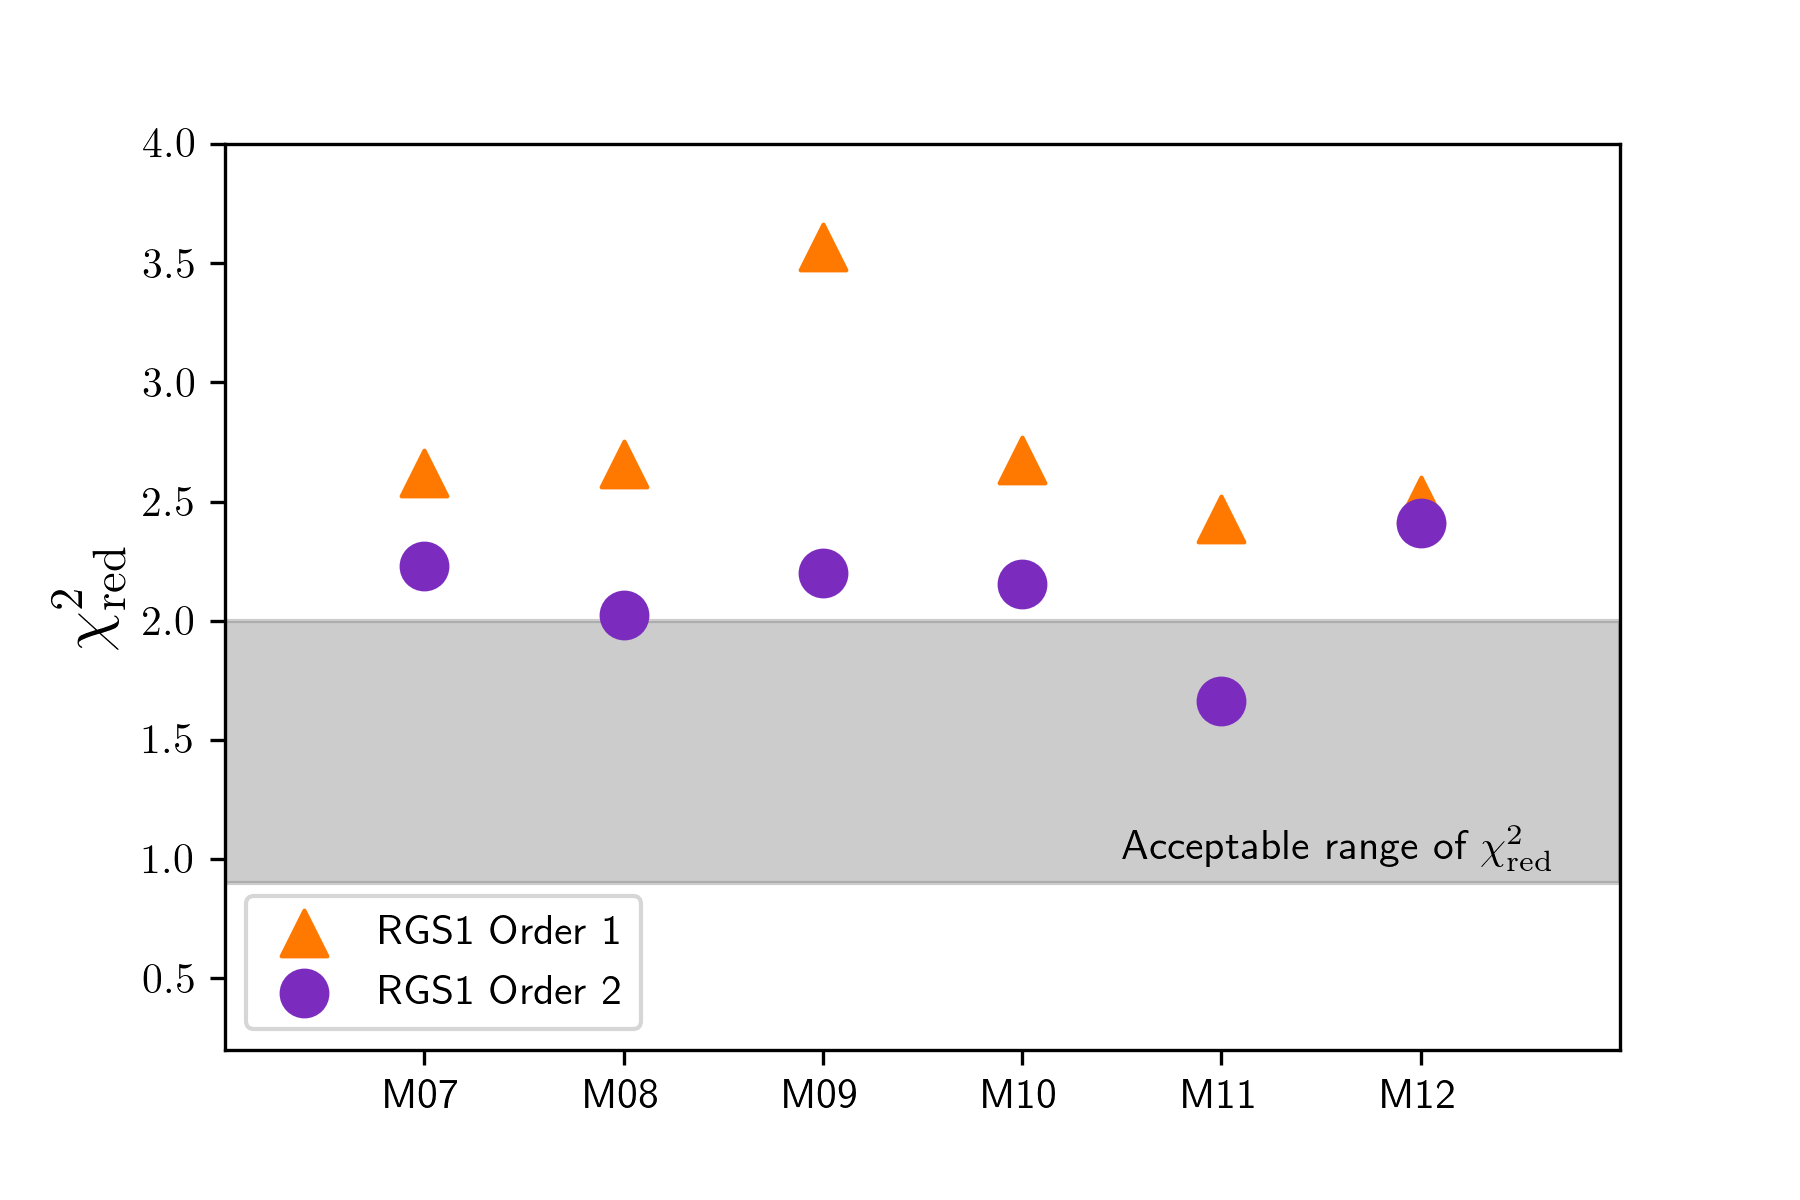
\includegraphics[width=0.85\textwidth]{mrvel-rgs1-chisq}
			\end{figure}
		
			The fitted spectra, along with the residuals are displayed as follows:
			\begin{figure}[h!]
				\centering
				\caption{Spectral fits for RGS1 spectra using model M07}
				\label{xmm:rgs1-m07}
				\subfloat[Order 1 \label{xmm:rgs1-m07:o1}]{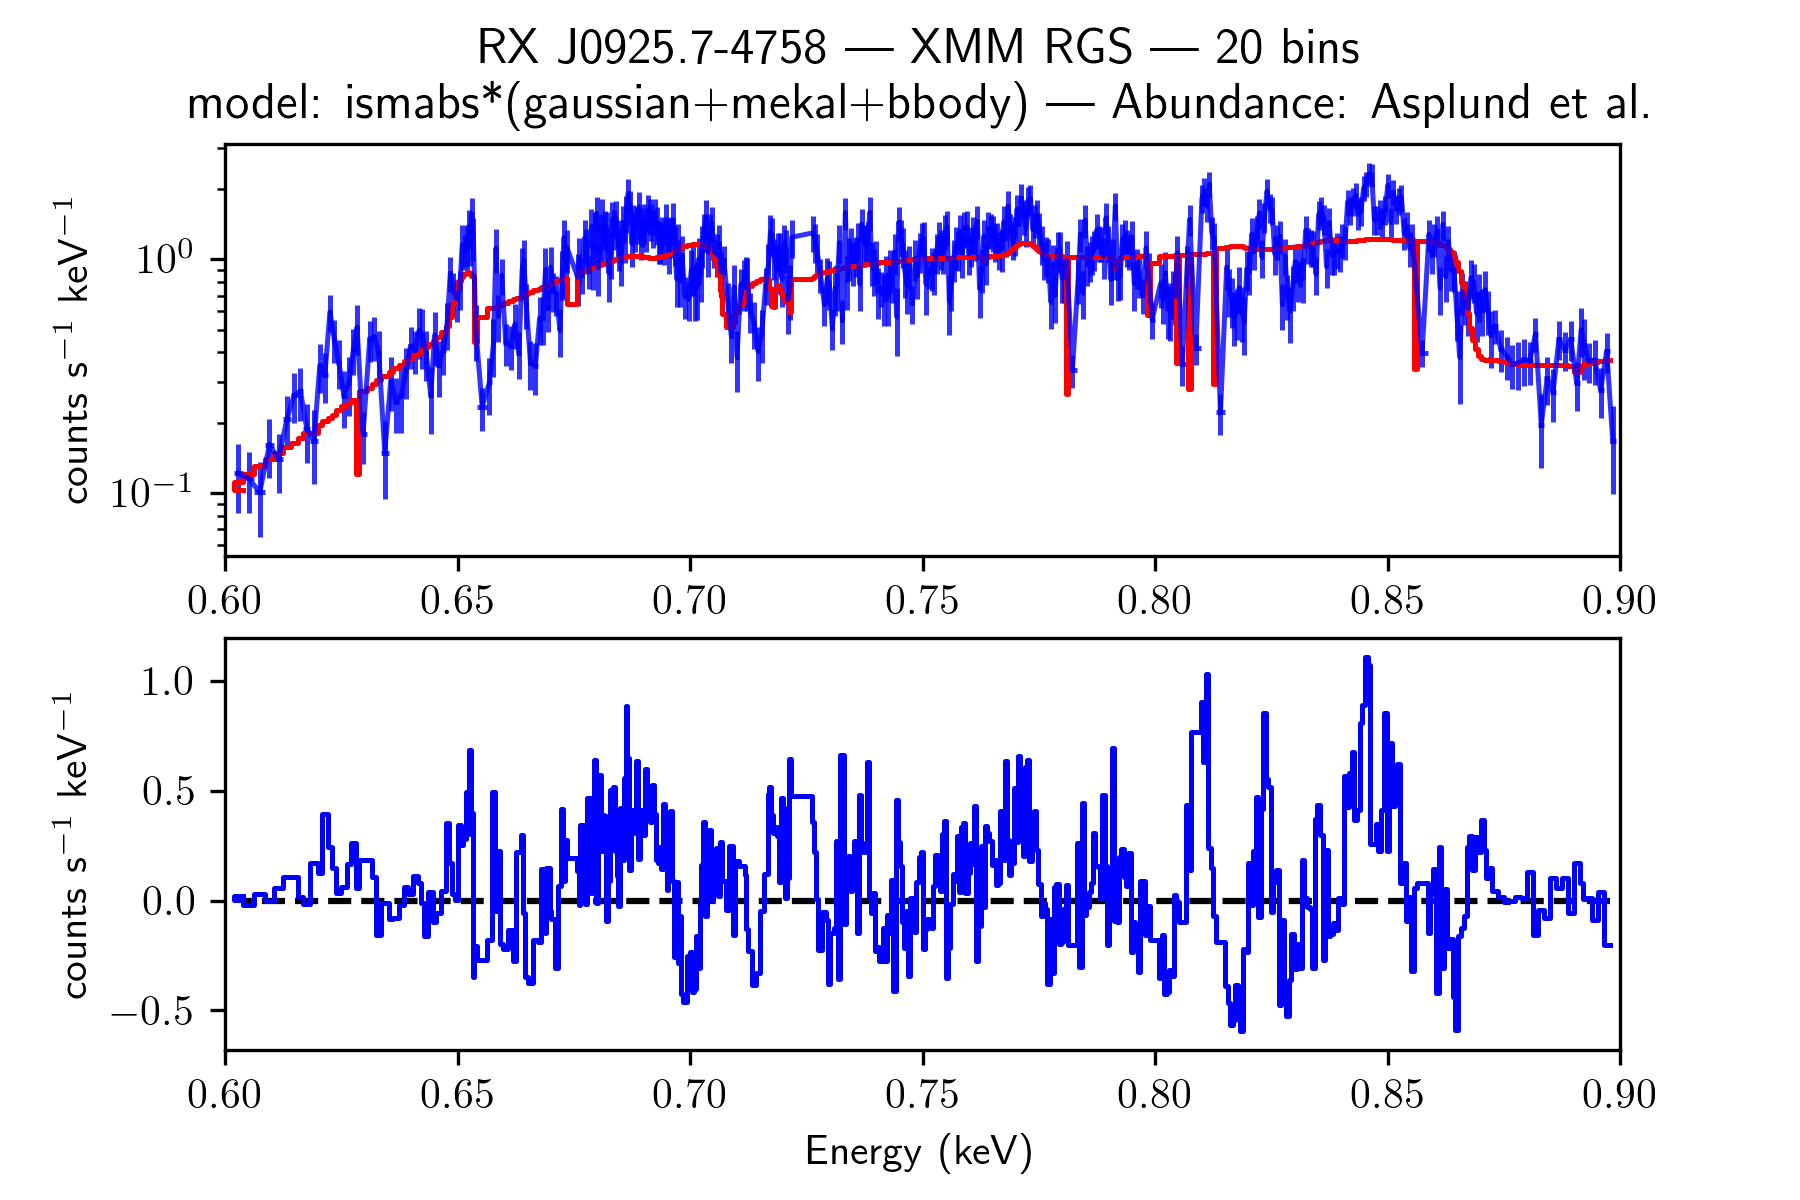
\includegraphics[width=0.45\textwidth]{mrvel-rgs1-o1-m07}} %\hfill
				\subfloat[Order 2 \label{xmm:rgs1-m07:o2}]{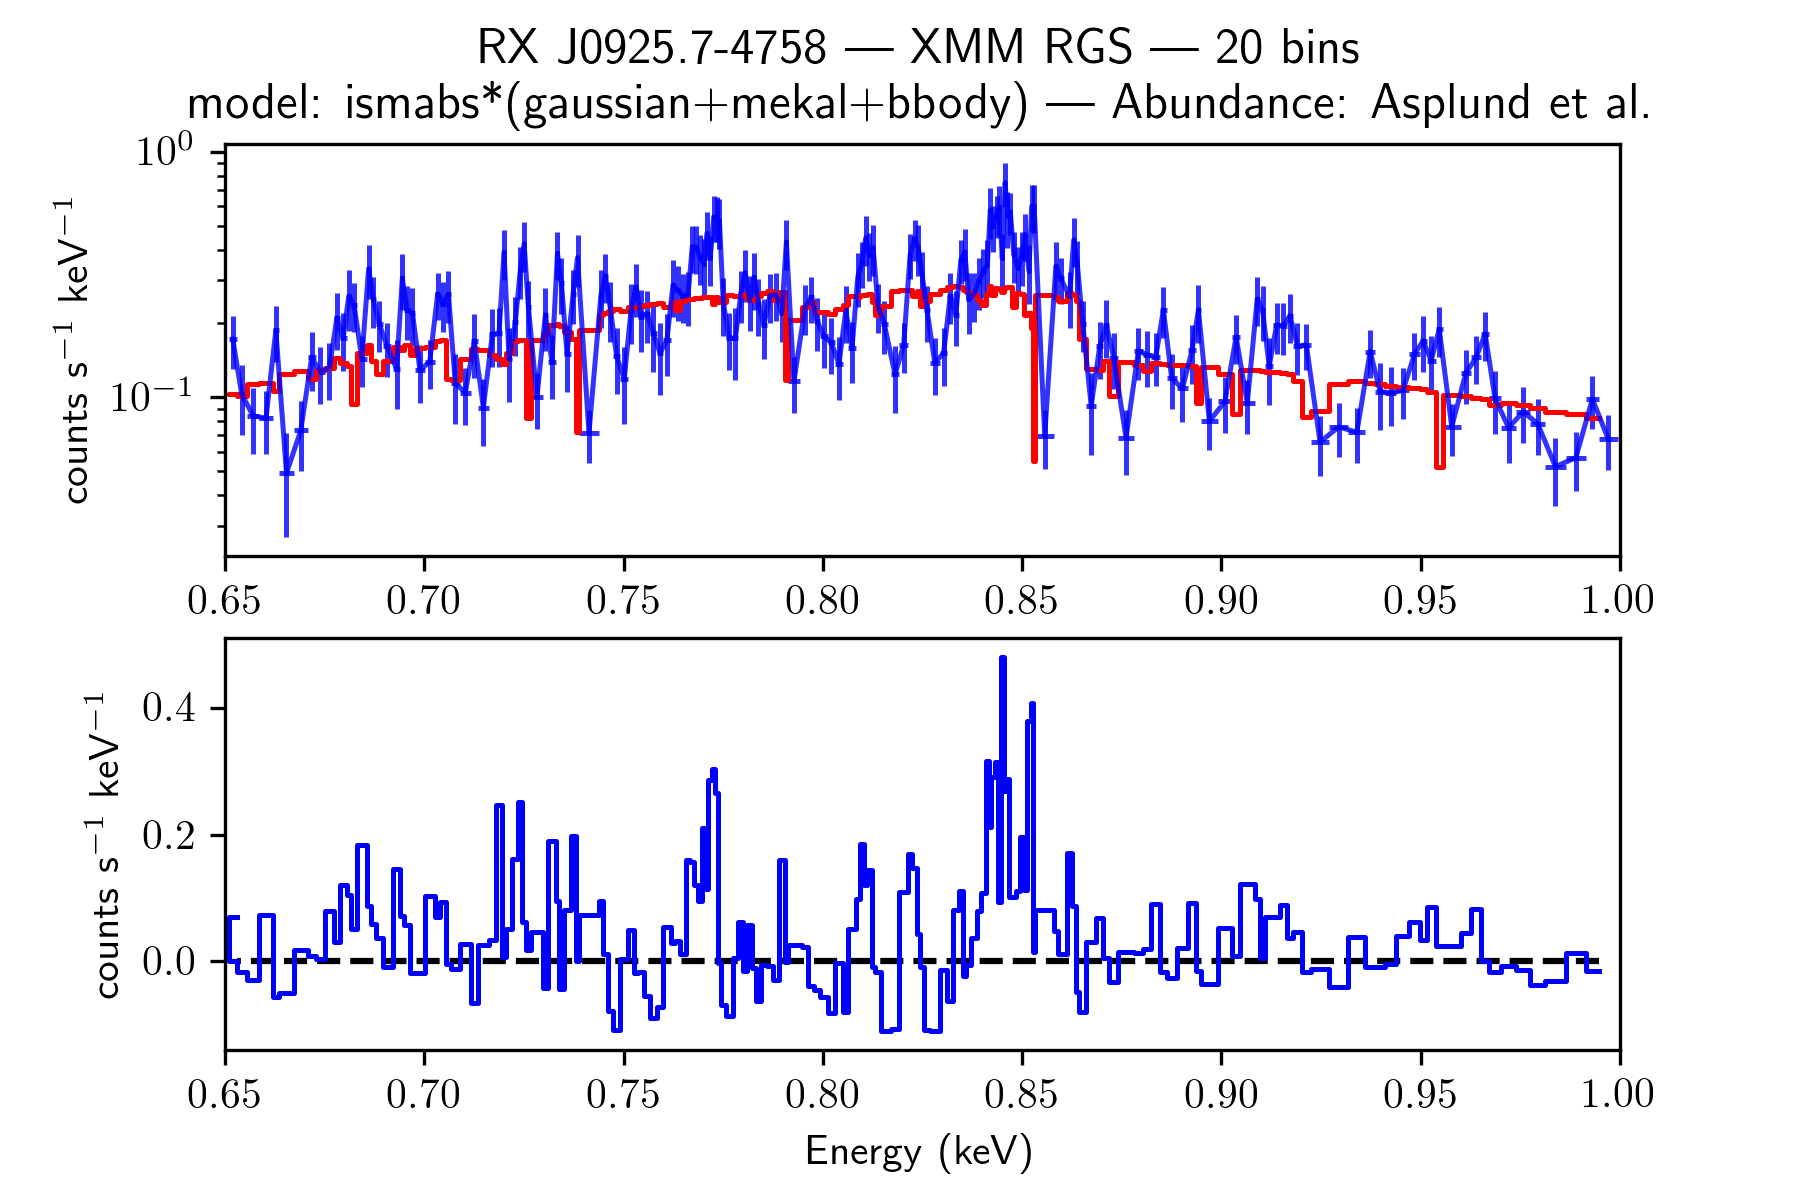
\includegraphics[width=0.45\textwidth]{mrvel-rgs1-o2-m07}} %\hfill
			\end{figure}
			\begin{figure}[h!]
				\centering
				\caption{Spectral fits for RGS1 spectra using model M08}
				\label{xmm:rgs1-m08}
				\subfloat[Order 1 \label{xmm:rgs1-m08:o1}]{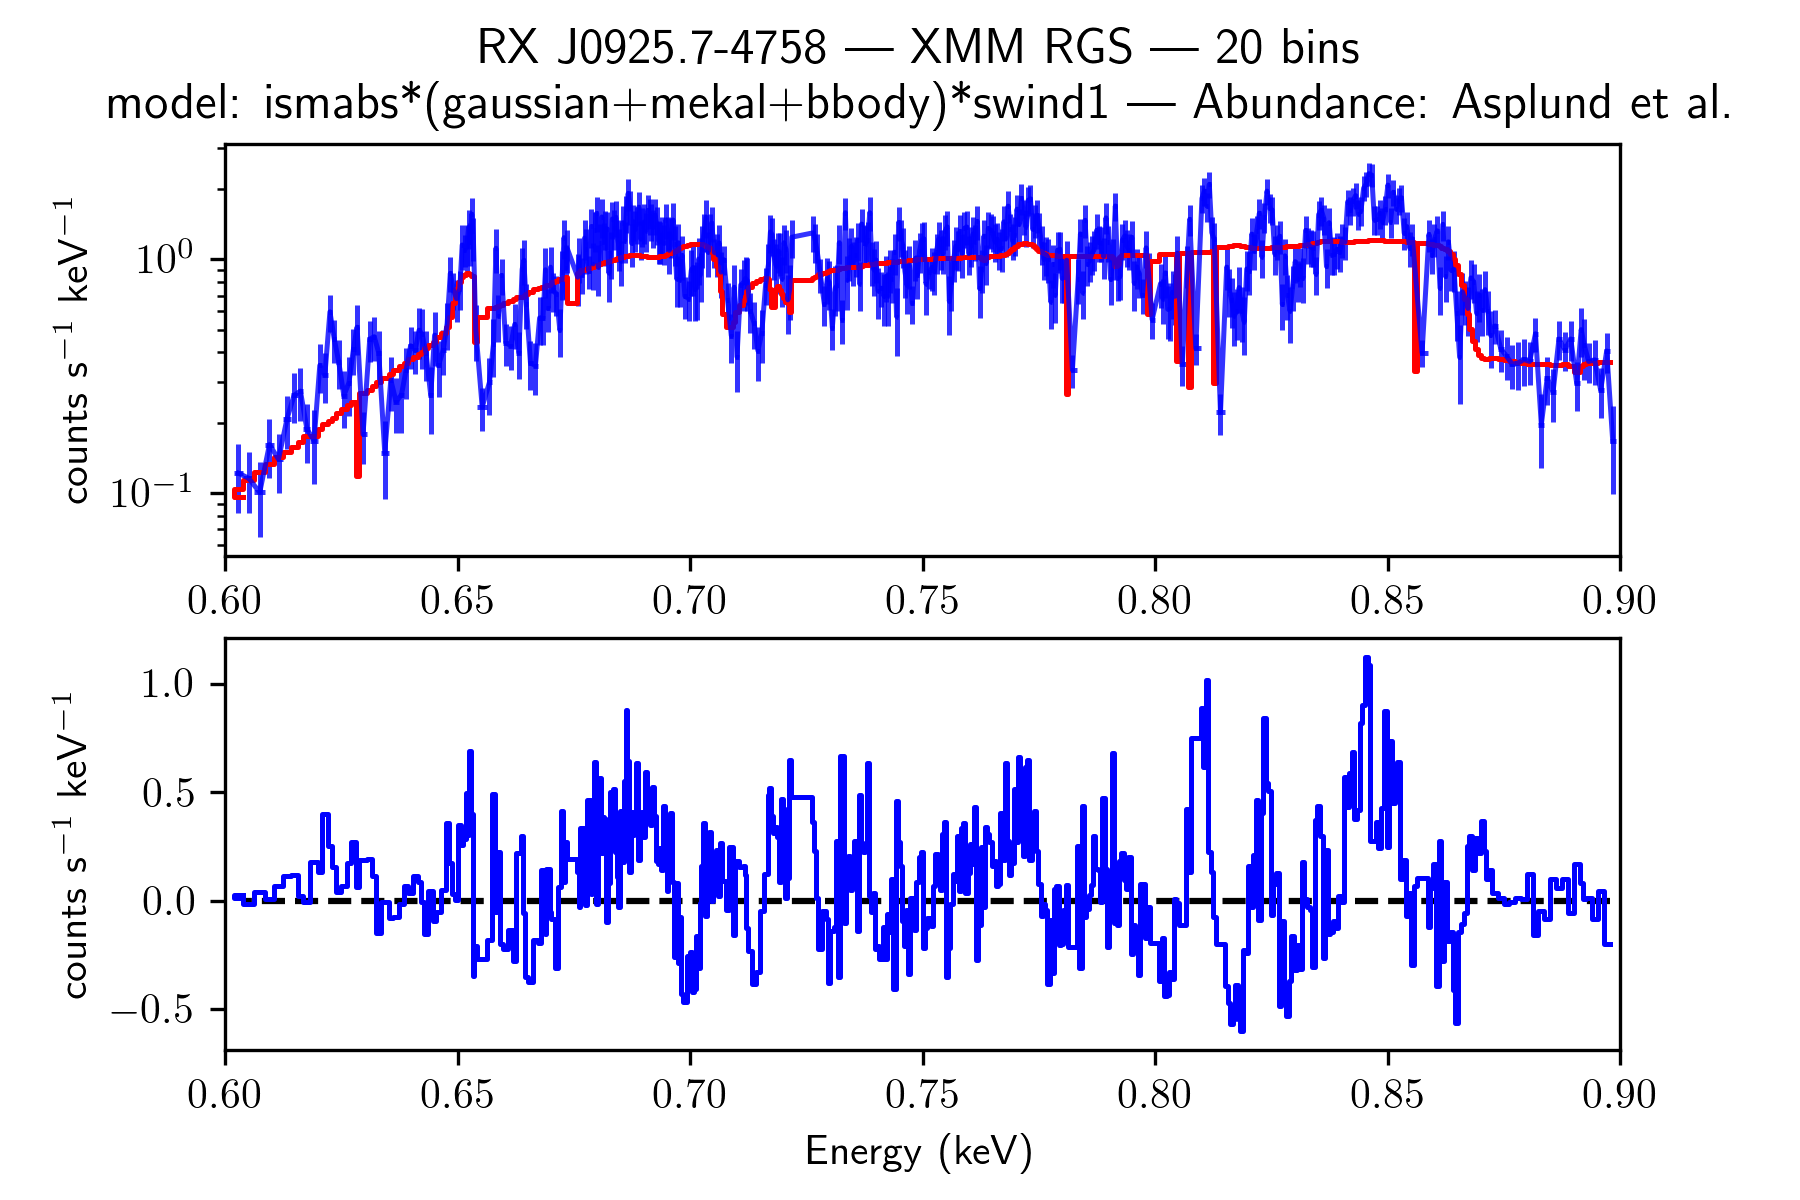
\includegraphics[width=0.45\textwidth]{mrvel-rgs1-o1-m08}} %\hfill
				\subfloat[Order 2 \label{xmm:rgs1-m08:o2}]{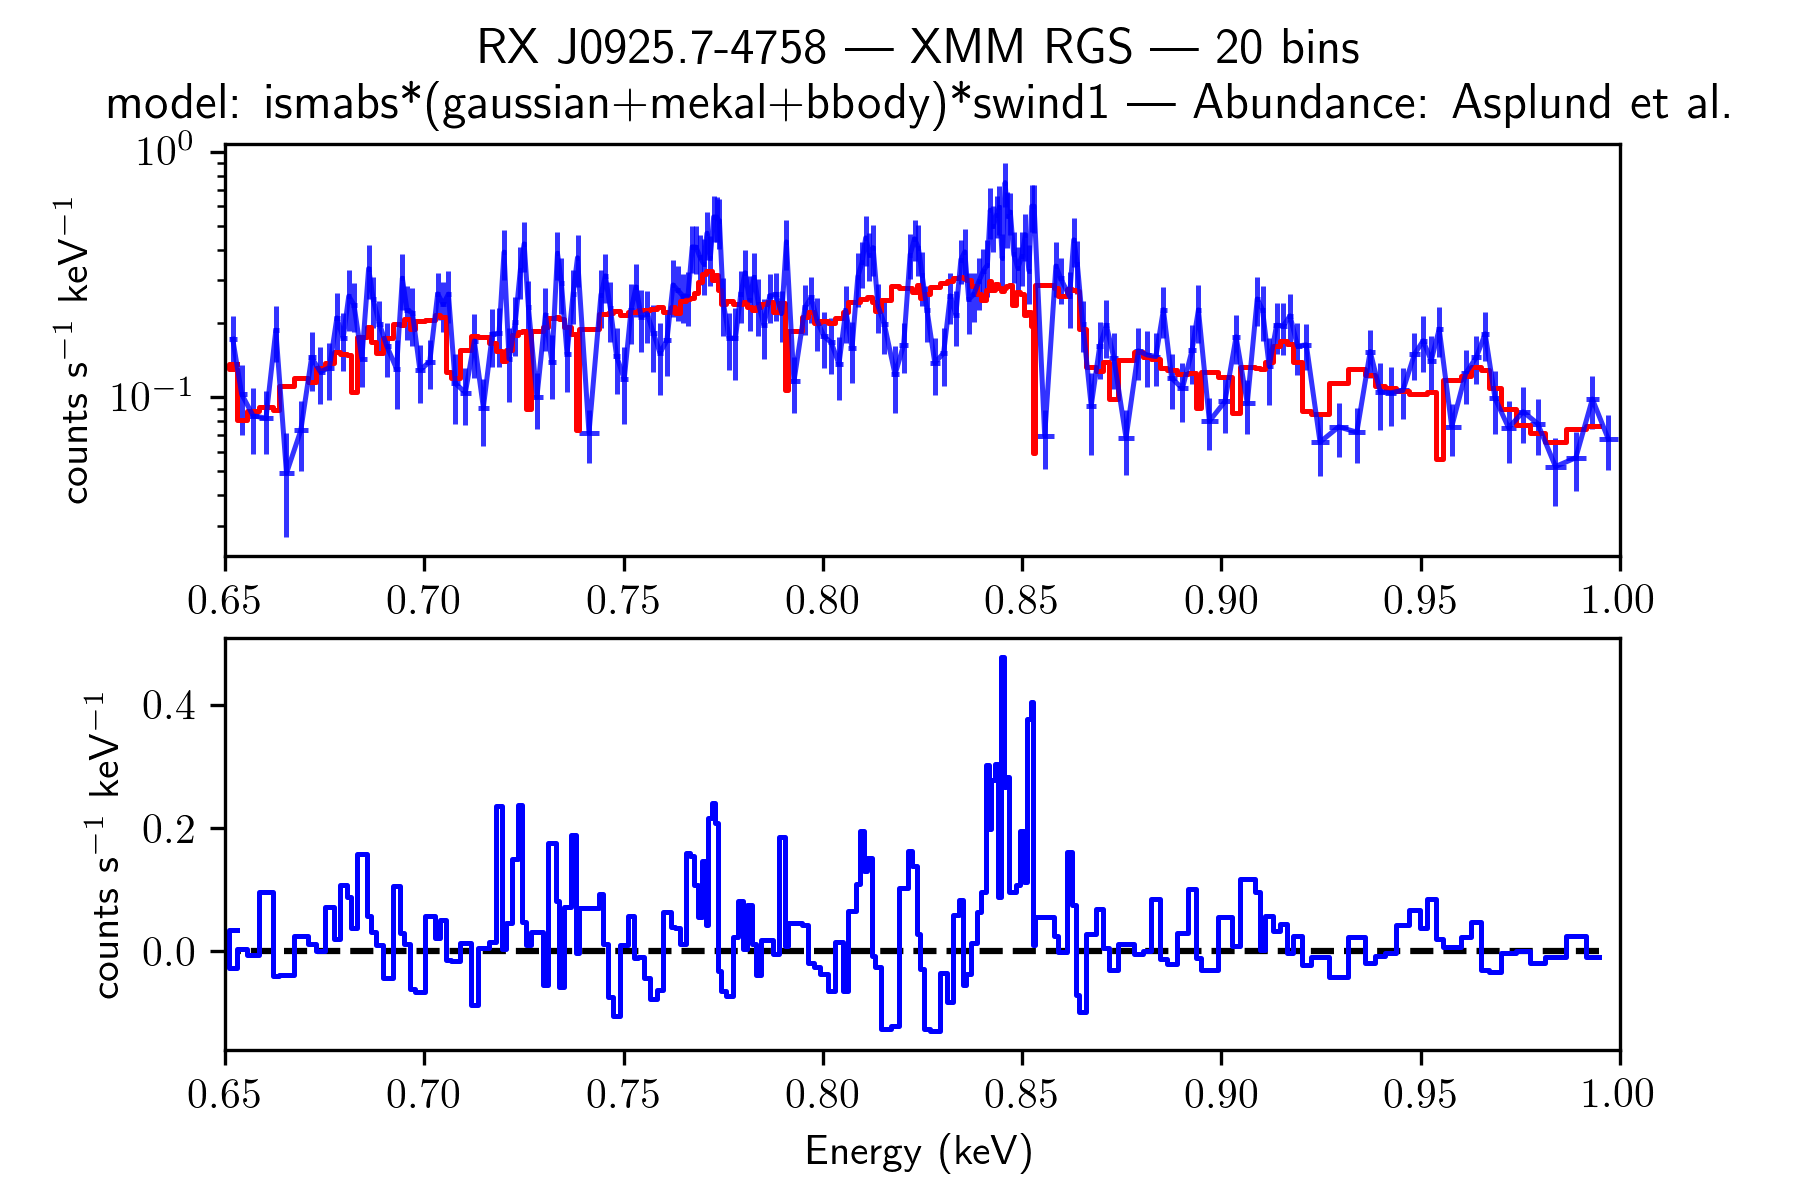
\includegraphics[width=0.45\textwidth]{mrvel-rgs1-o2-m08}} %\hfill
			\end{figure}
			\begin{figure}[h!]
				\centering
				\caption{Spectral fits for RGS1 spectra using model M09}
				\label{xmm:rgs1-m09}
				\subfloat[Order 1 \label{xmm:rgs1-m09:o1}]{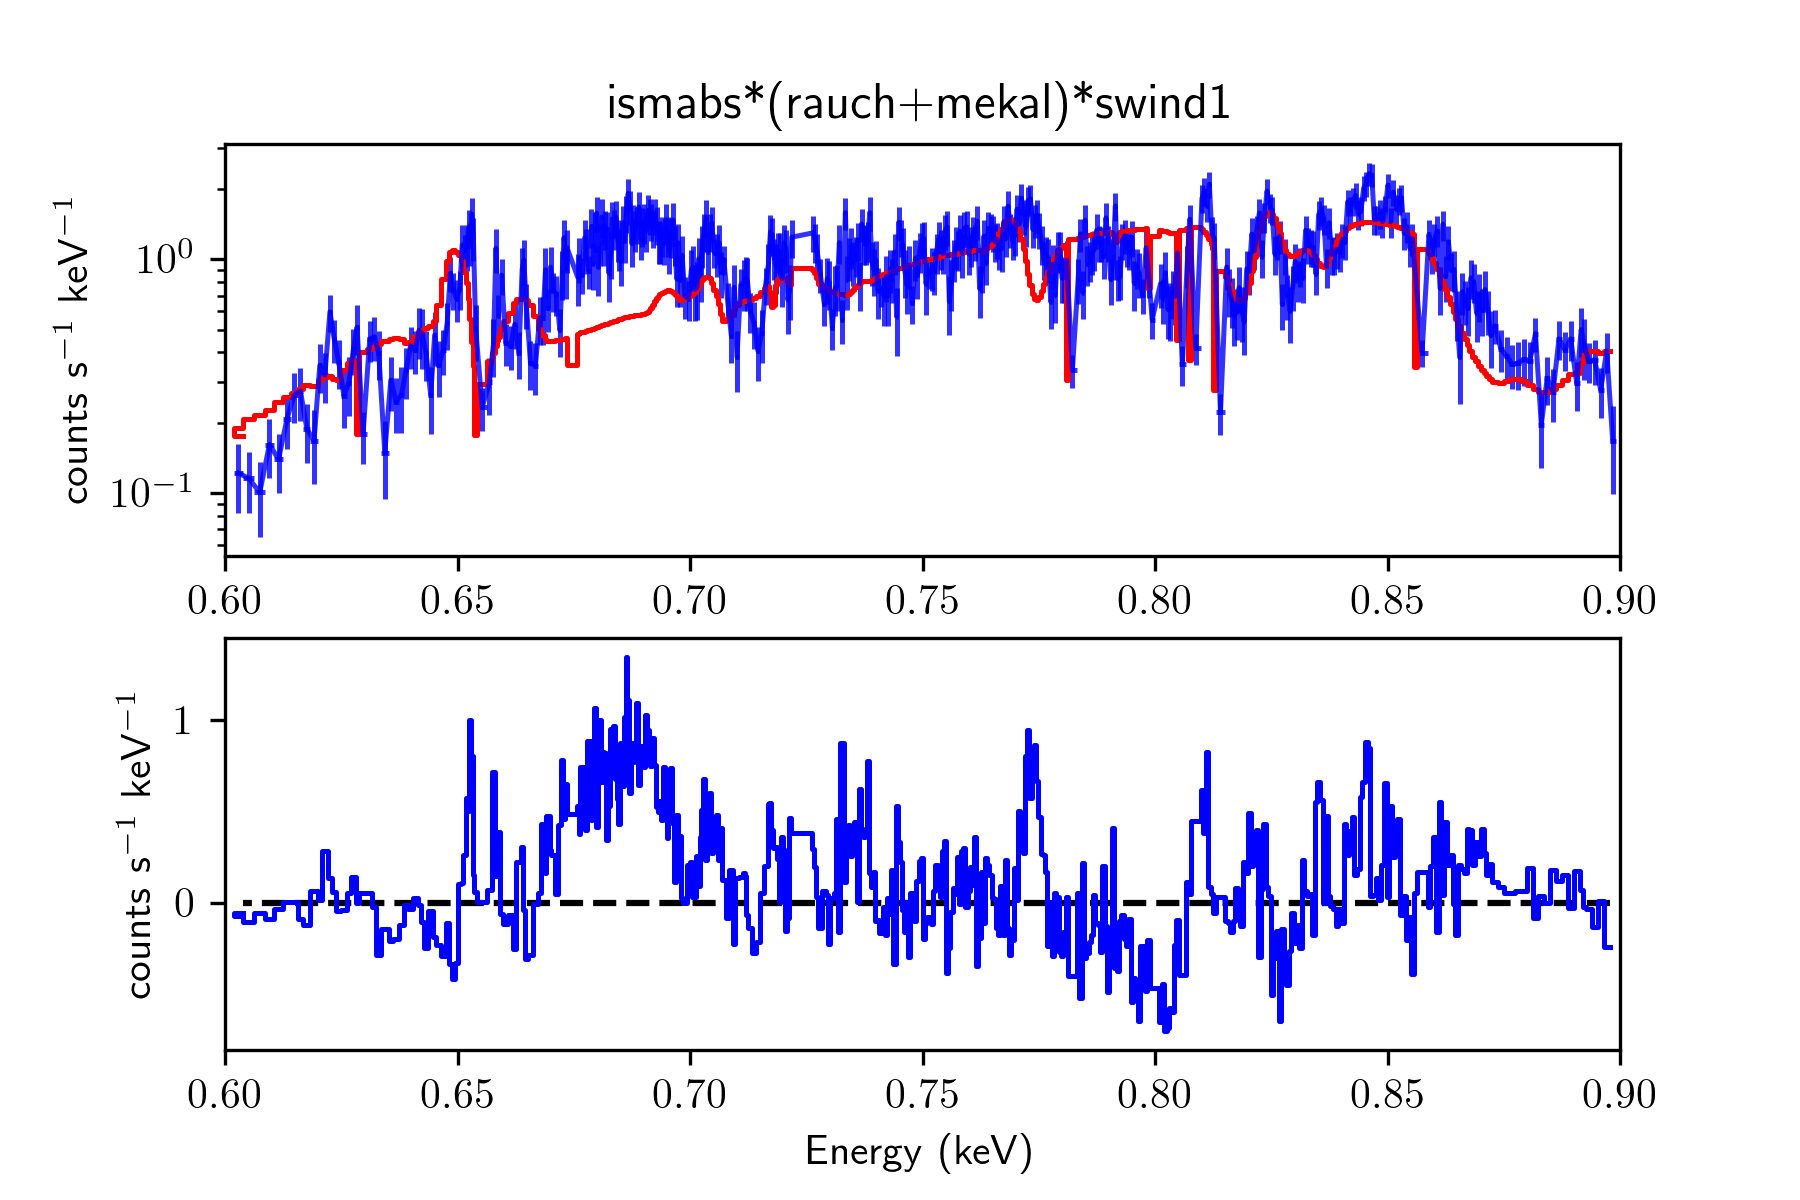
\includegraphics[width=0.45\textwidth]{mrvel-rgs1-o1-m09}} %\hfill
				\subfloat[Order 2 \label{xmm:rgs1-m09:o2}]{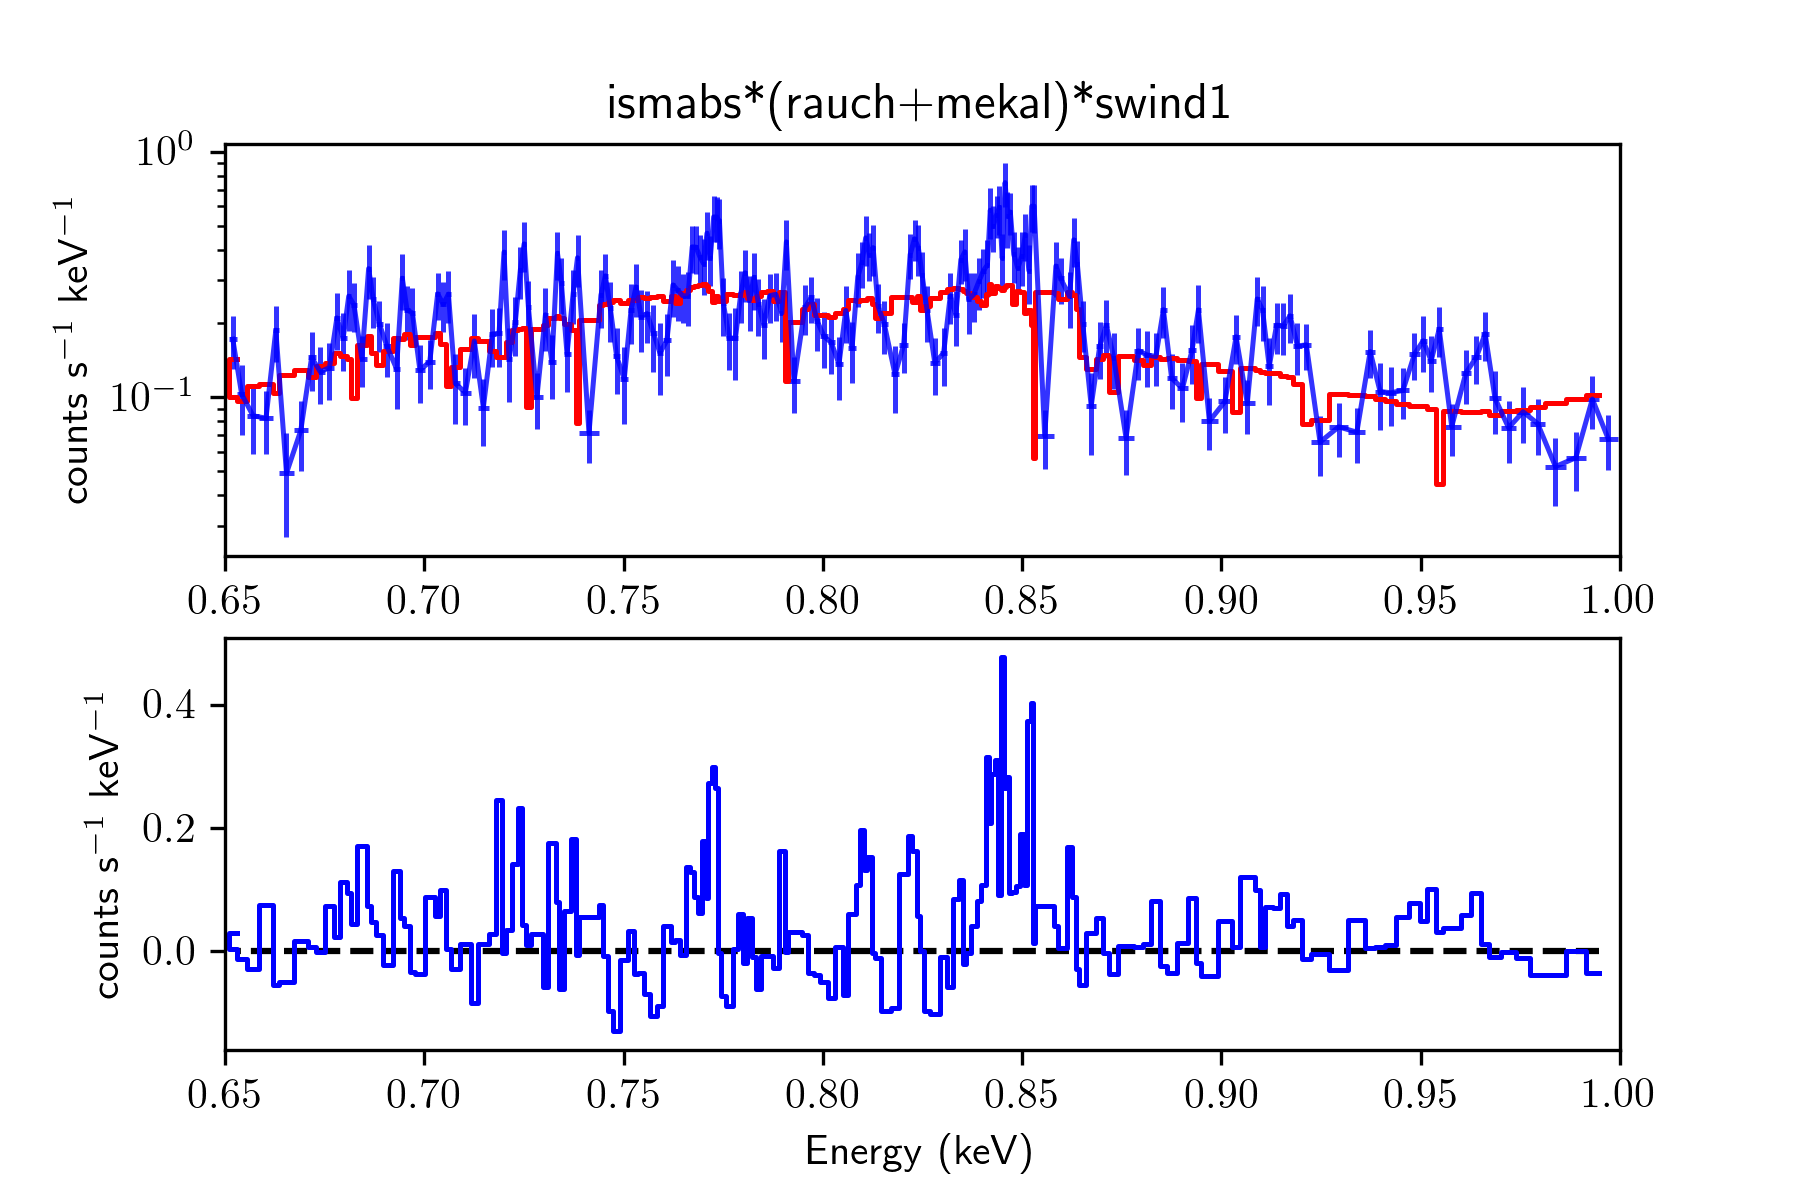
\includegraphics[width=0.45\textwidth]{mrvel-rgs1-o2-m09}} %\hfill
			\end{figure}
			\begin{figure}[h!]
				\centering
				\caption{Spectral fits for RGS1 spectra using model M10}
				\label{xmm:rgs1-m10}
				\subfloat[Order 1 \label{xmm:rgs1-m10:o1}]{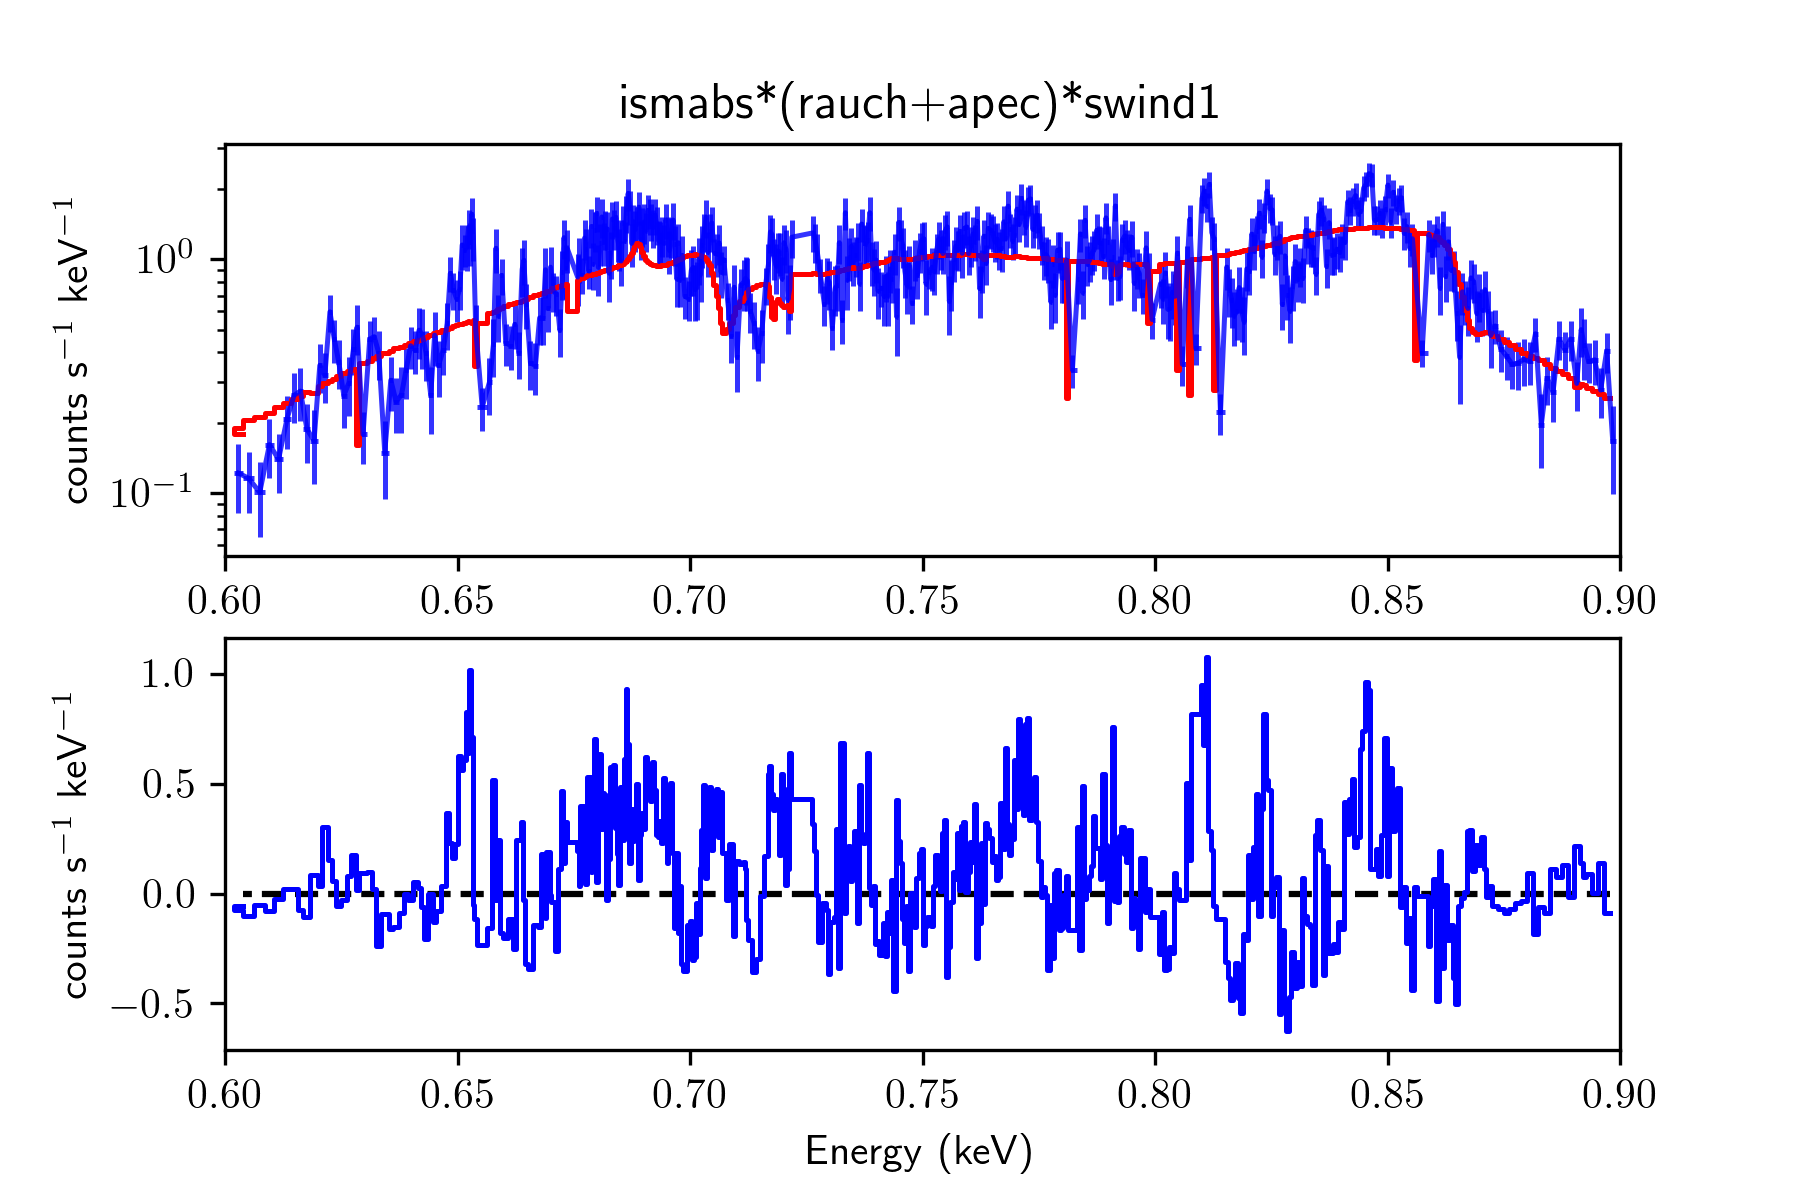
\includegraphics[width=0.45\textwidth]{mrvel-rgs1-o1-m10}} %\hfill
				\subfloat[Order 2 \label{xmm:rgs1-m10:o2}]{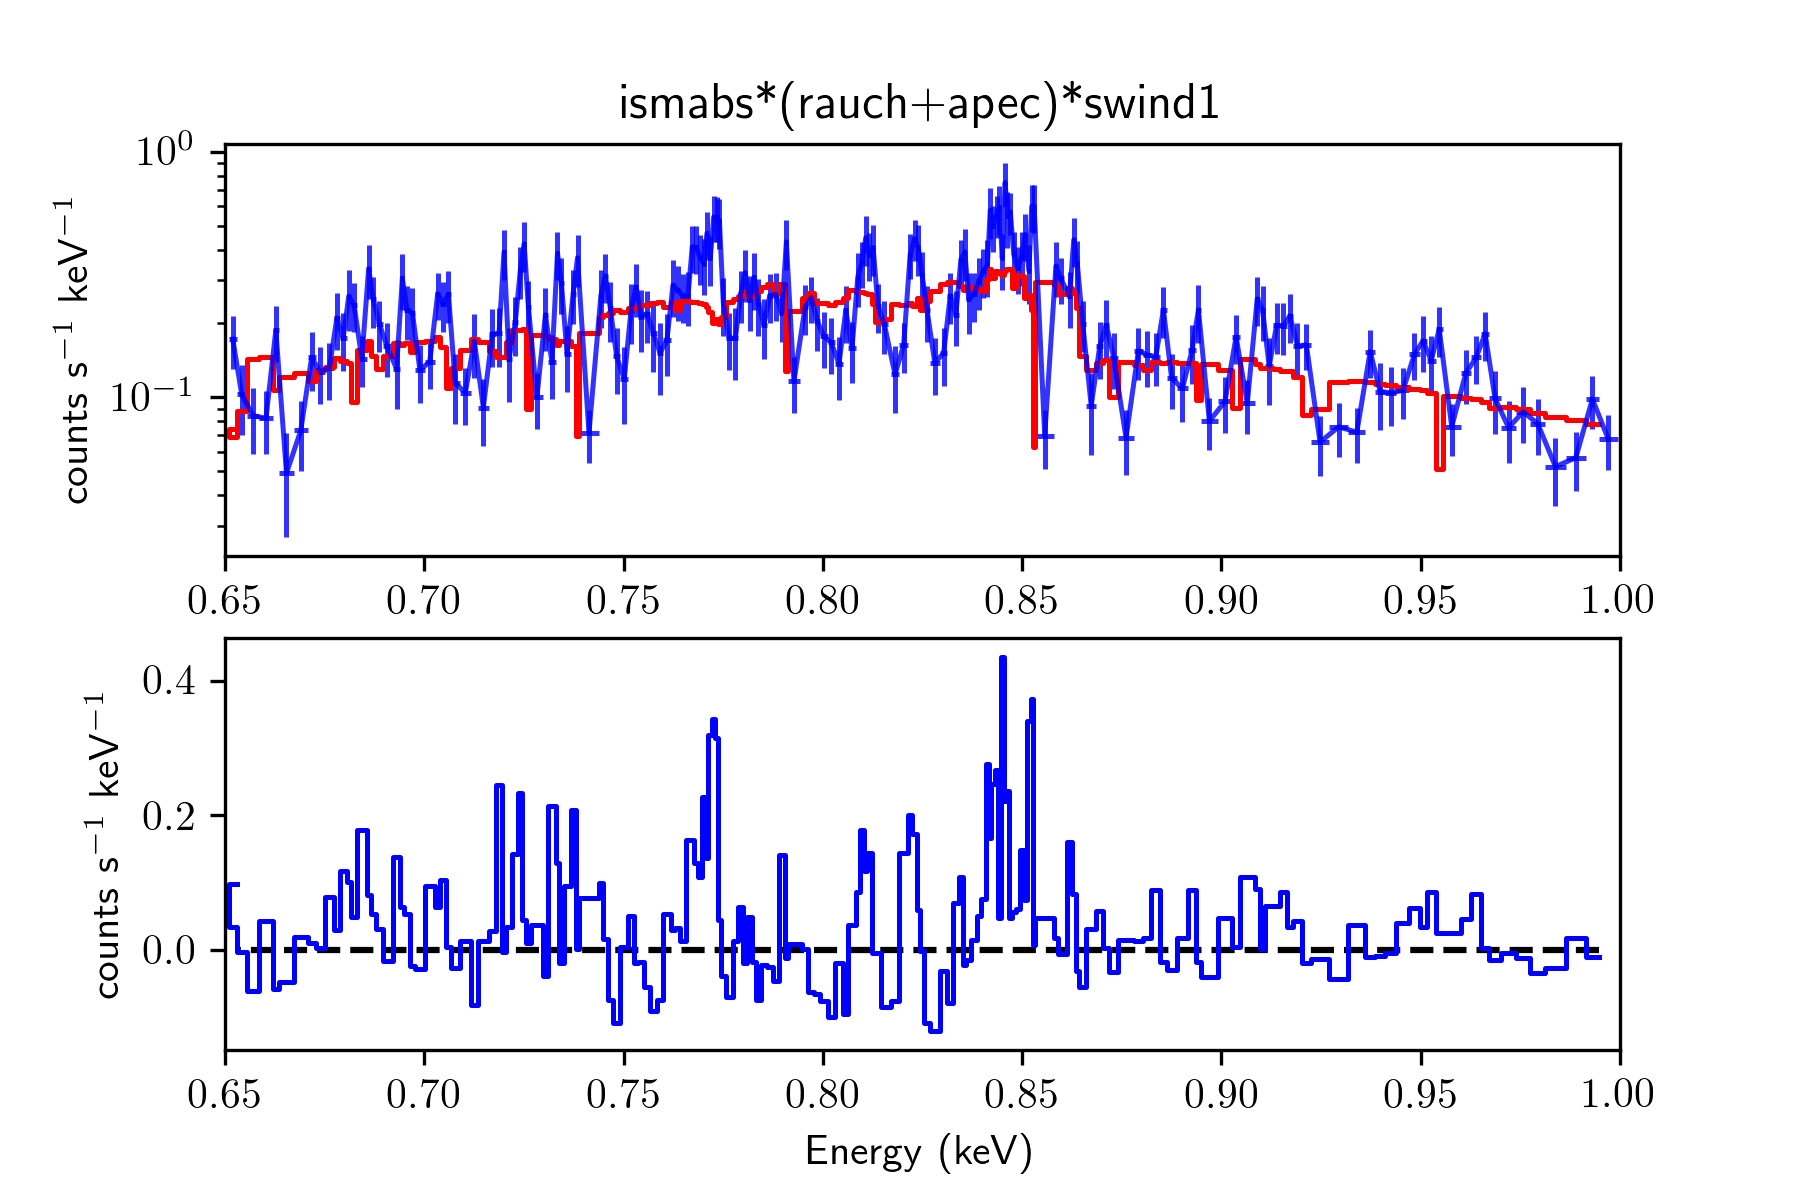
\includegraphics[width=0.45\textwidth]{mrvel-rgs1-o2-m10}} %\hfill
			\end{figure}
			\begin{figure}[h!]
				\centering
				\caption{Spectral fits for RGS1 spectra using model M11}
				\label{xmm:rgs1-m11}
				\subfloat[Order 1 \label{xmm:rgs1-m11:o1}]{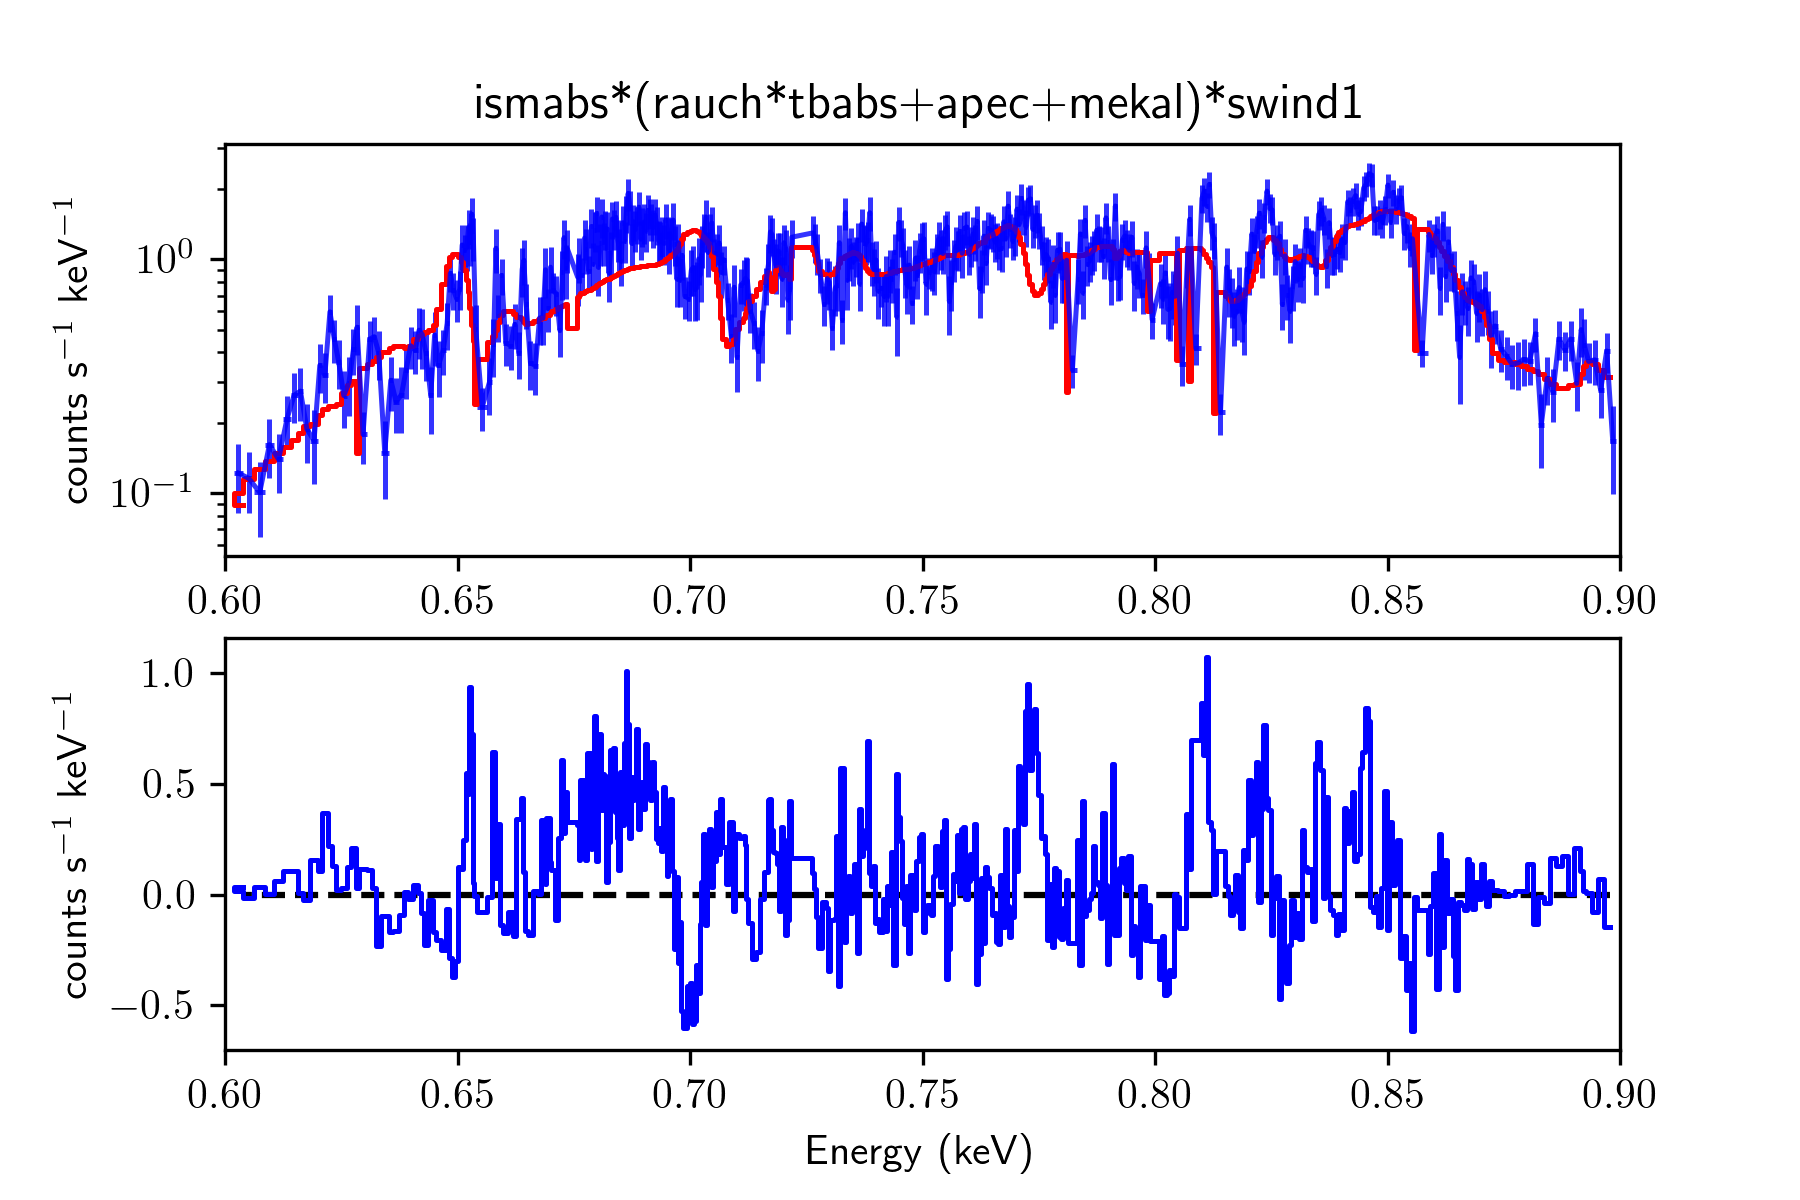
\includegraphics[width=0.45\textwidth]{mrvel-rgs1-o1-m11}} %\hfill
				\subfloat[Order 2 \label{xmm:rgs1-m11:o2}]{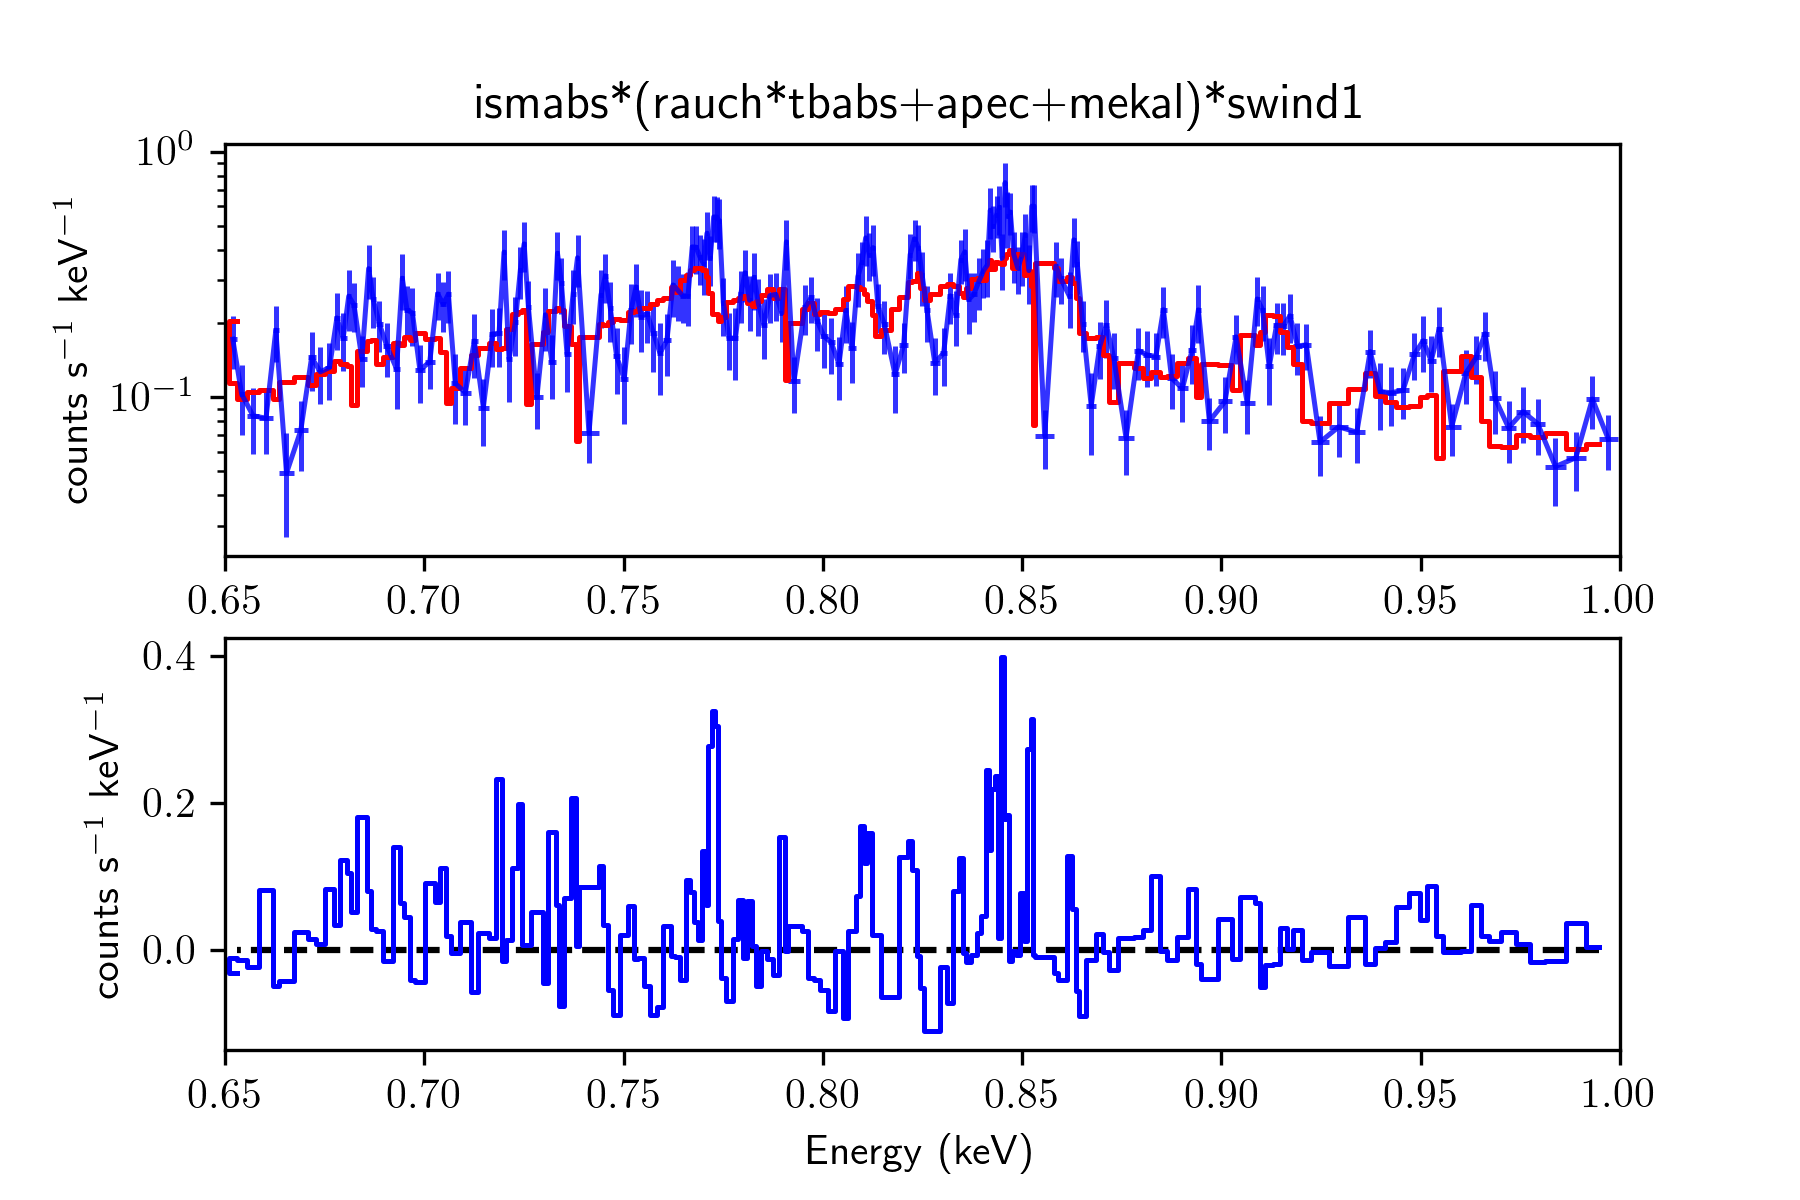
\includegraphics[width=0.45\textwidth]{mrvel-rgs1-o2-m11}} %\hfill
			\end{figure}
			\begin{figure}[h!]
				\centering
				\caption{Spectral fits for RGS1 spectra using model M12}
				\label{xmm:rgs1-m12}
				\subfloat[Order 1 \label{xmm:rgs1-m12:o1}]{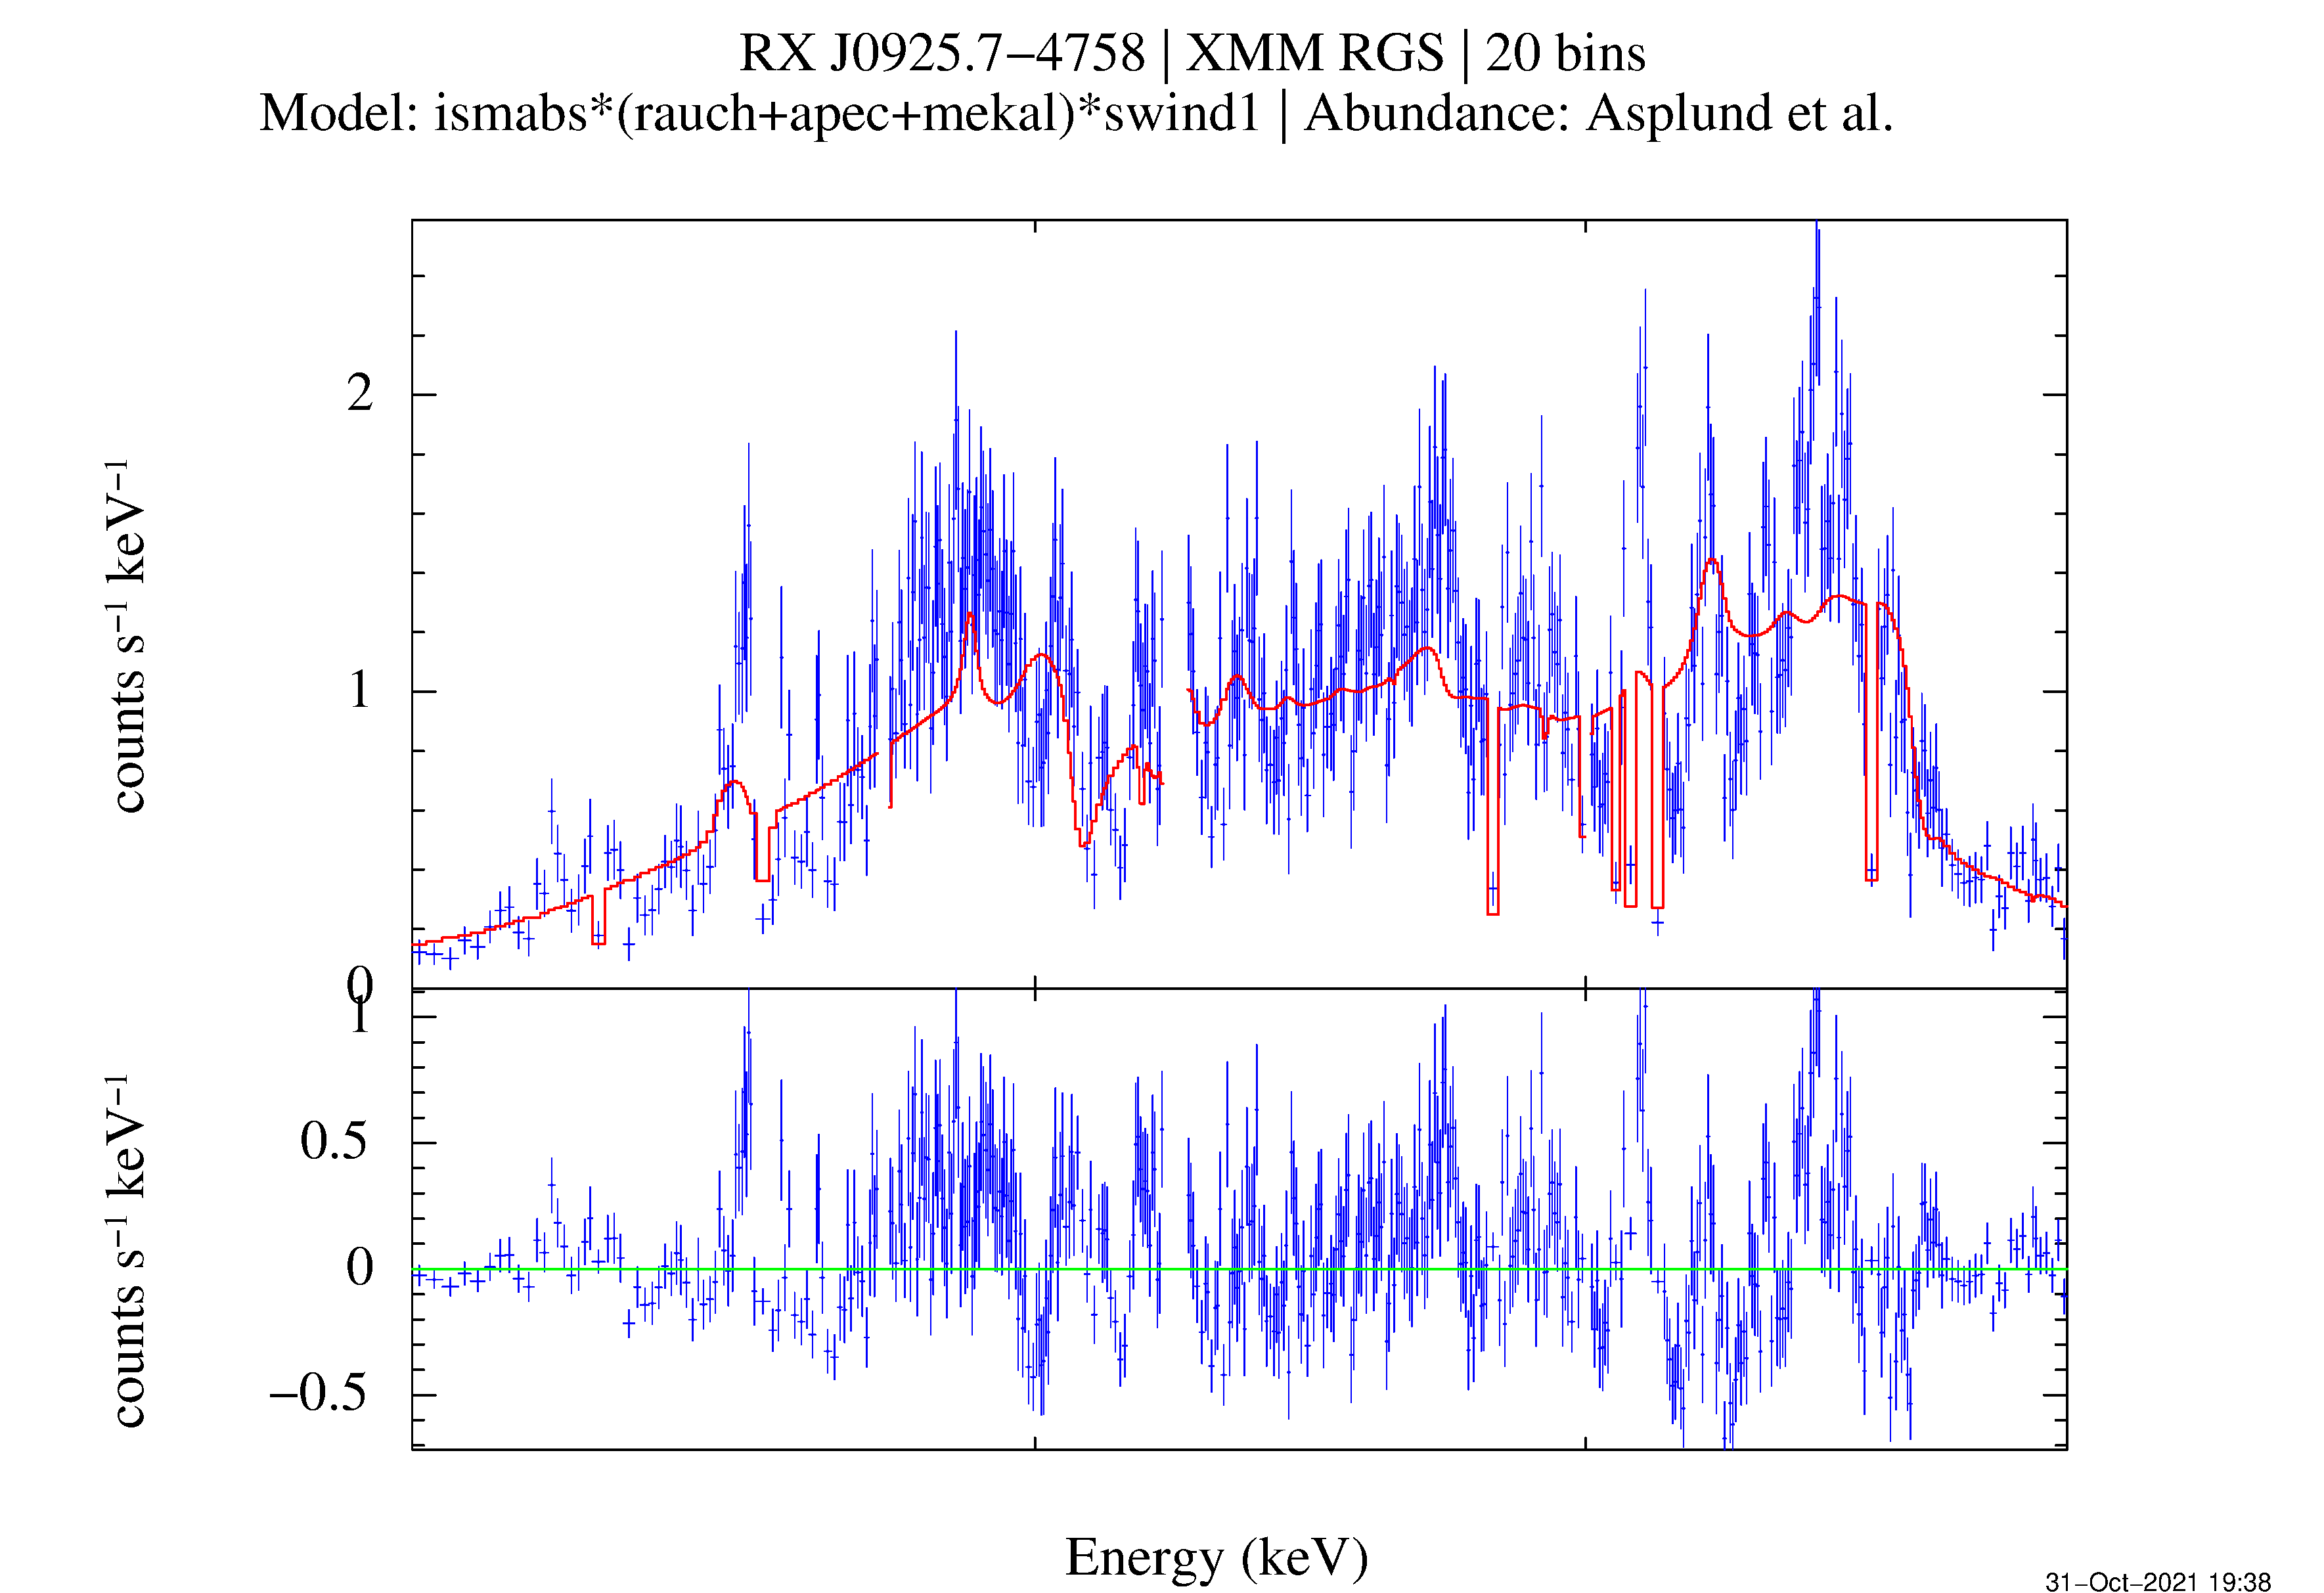
\includegraphics[width=0.45\textwidth]{mrvel-rgs1-o1-m12}} %\hfill
				\subfloat[Order 2 \label{xmm:rgs1-m12:o2}]{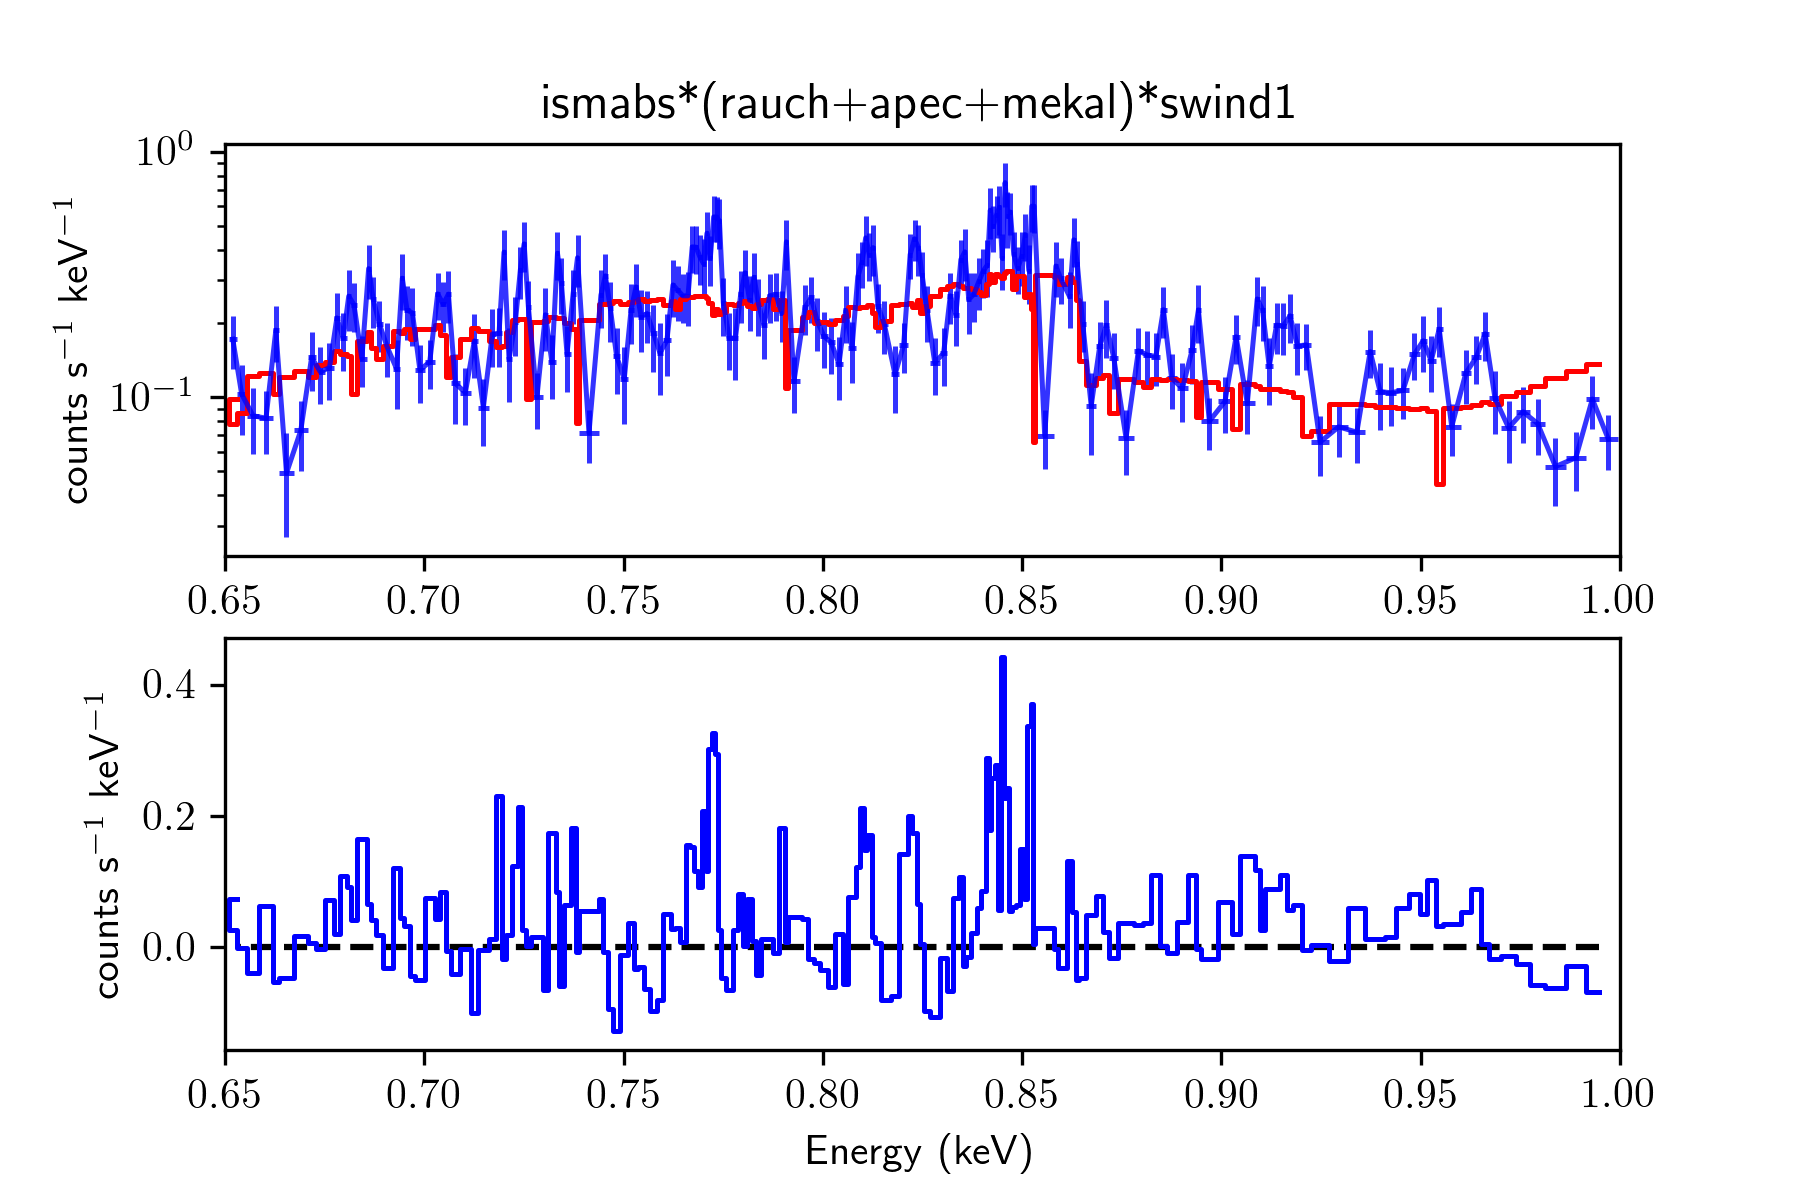
\includegraphics[width=0.45\textwidth]{mrvel-rgs1-o2-m12}} %\hfill
			\end{figure}
		
		\clearpage
		\subsection{Fitting of RGS2 Spectra} \label{hi-resolution:analysis:rgs2}
			Here as well the best fits for both diffraction orders were obtained using the model M11. This seems to suggest that model M11 might be the best candidate model for RX J0925.7-4758. All the other models yield $\chi^2_\text{red}$ to be outside the acceptable range, with the exception of the model M08, which lies almost on the borderline. The trend shown by the $\chi^2_\text{red}$ across all the models considered here are shown in figure \ref{fig:mrvel-rgs2-chisq}.
			
			\begin{figure}[h!]
				\centering
				\caption{$\chi^2_\text{red}$ trend for RX J0925.7-4758 spectra from RGS2 instrument}
				\label{fig:mrvel-rgs2-chisq}
				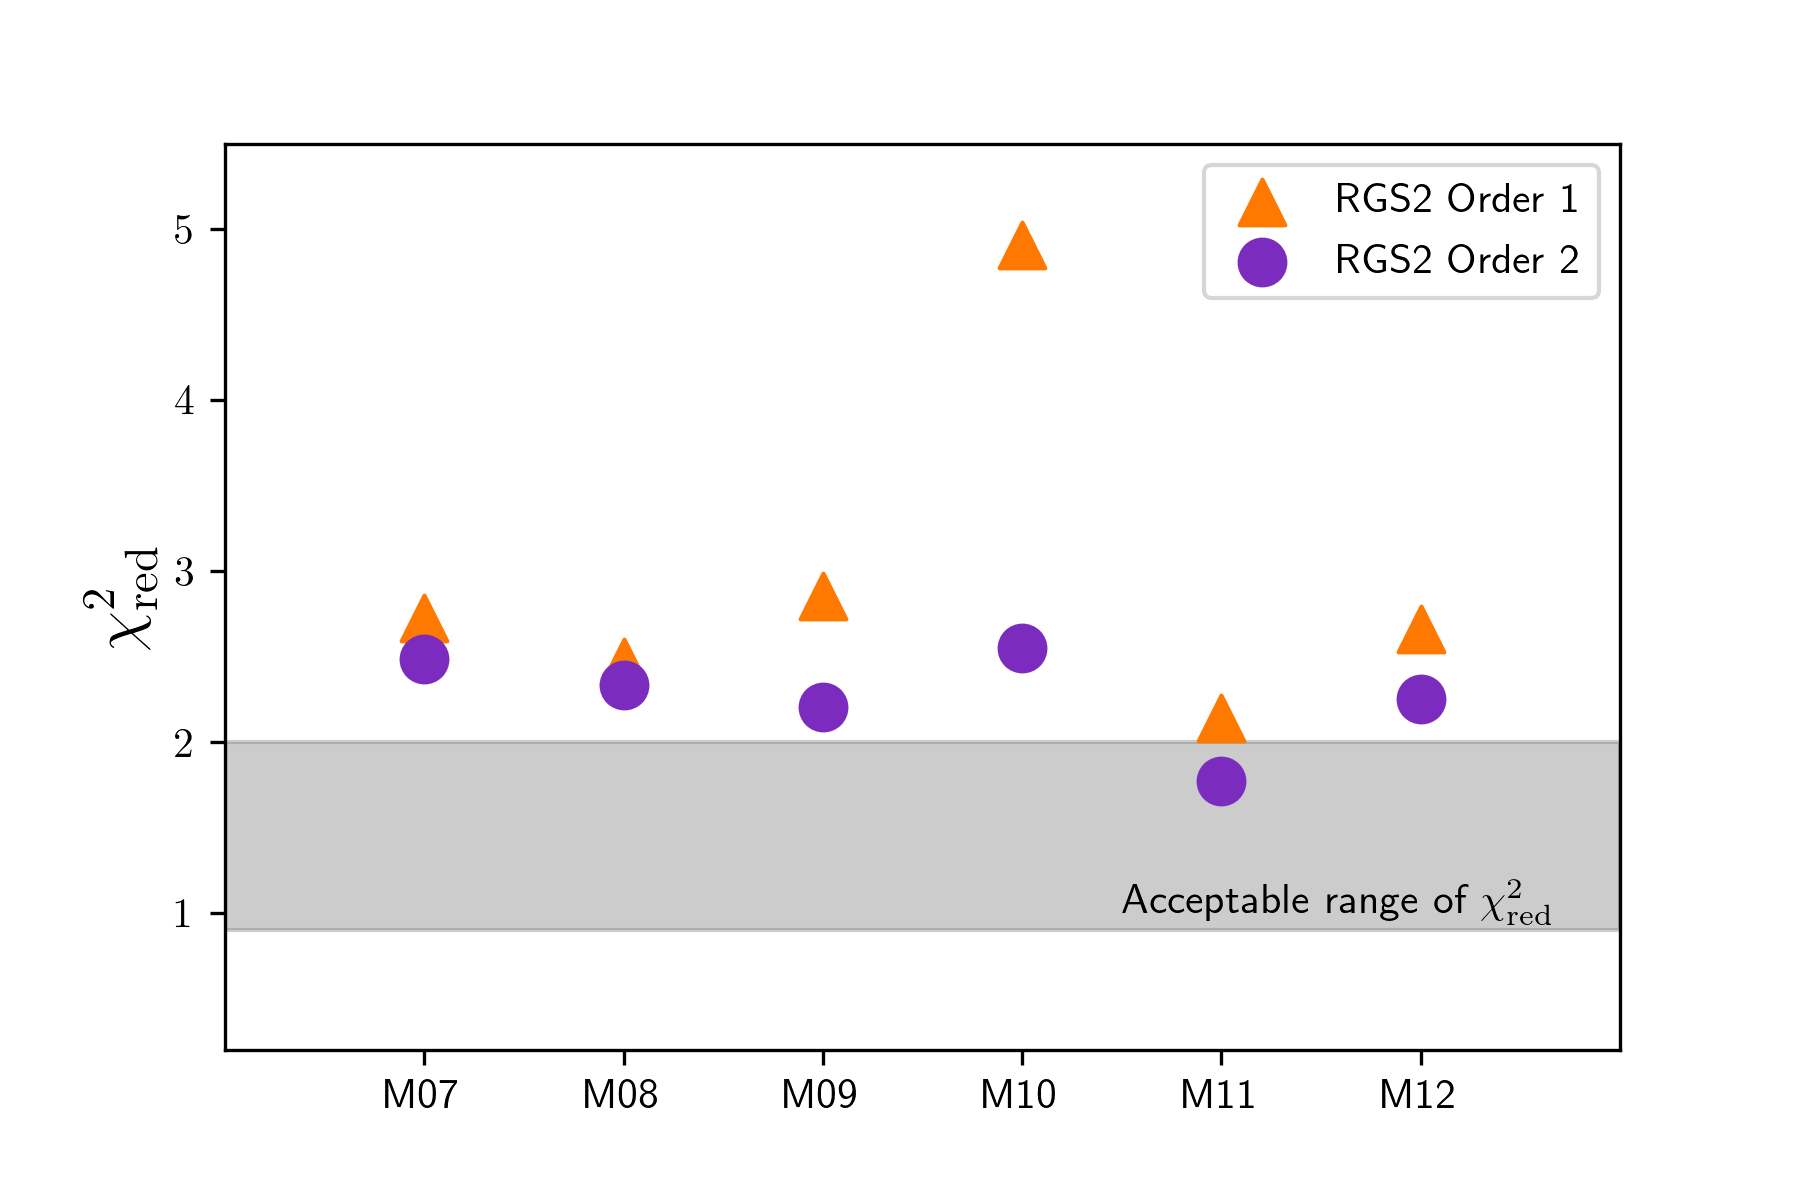
\includegraphics[width=0.85\textwidth]{mrvel-rgs2-chisq}
			\end{figure}
			The fitted spectra, along with the residuals are displayed as follows:
			\begin{figure}[h!]
				\centering
				\caption{Spectral fits for RGS2 spectra using model M07}
				\label{xmm:rgs2-m07}
				\subfloat[Order 1 \label{xmm:rgs2-m07:o1}]{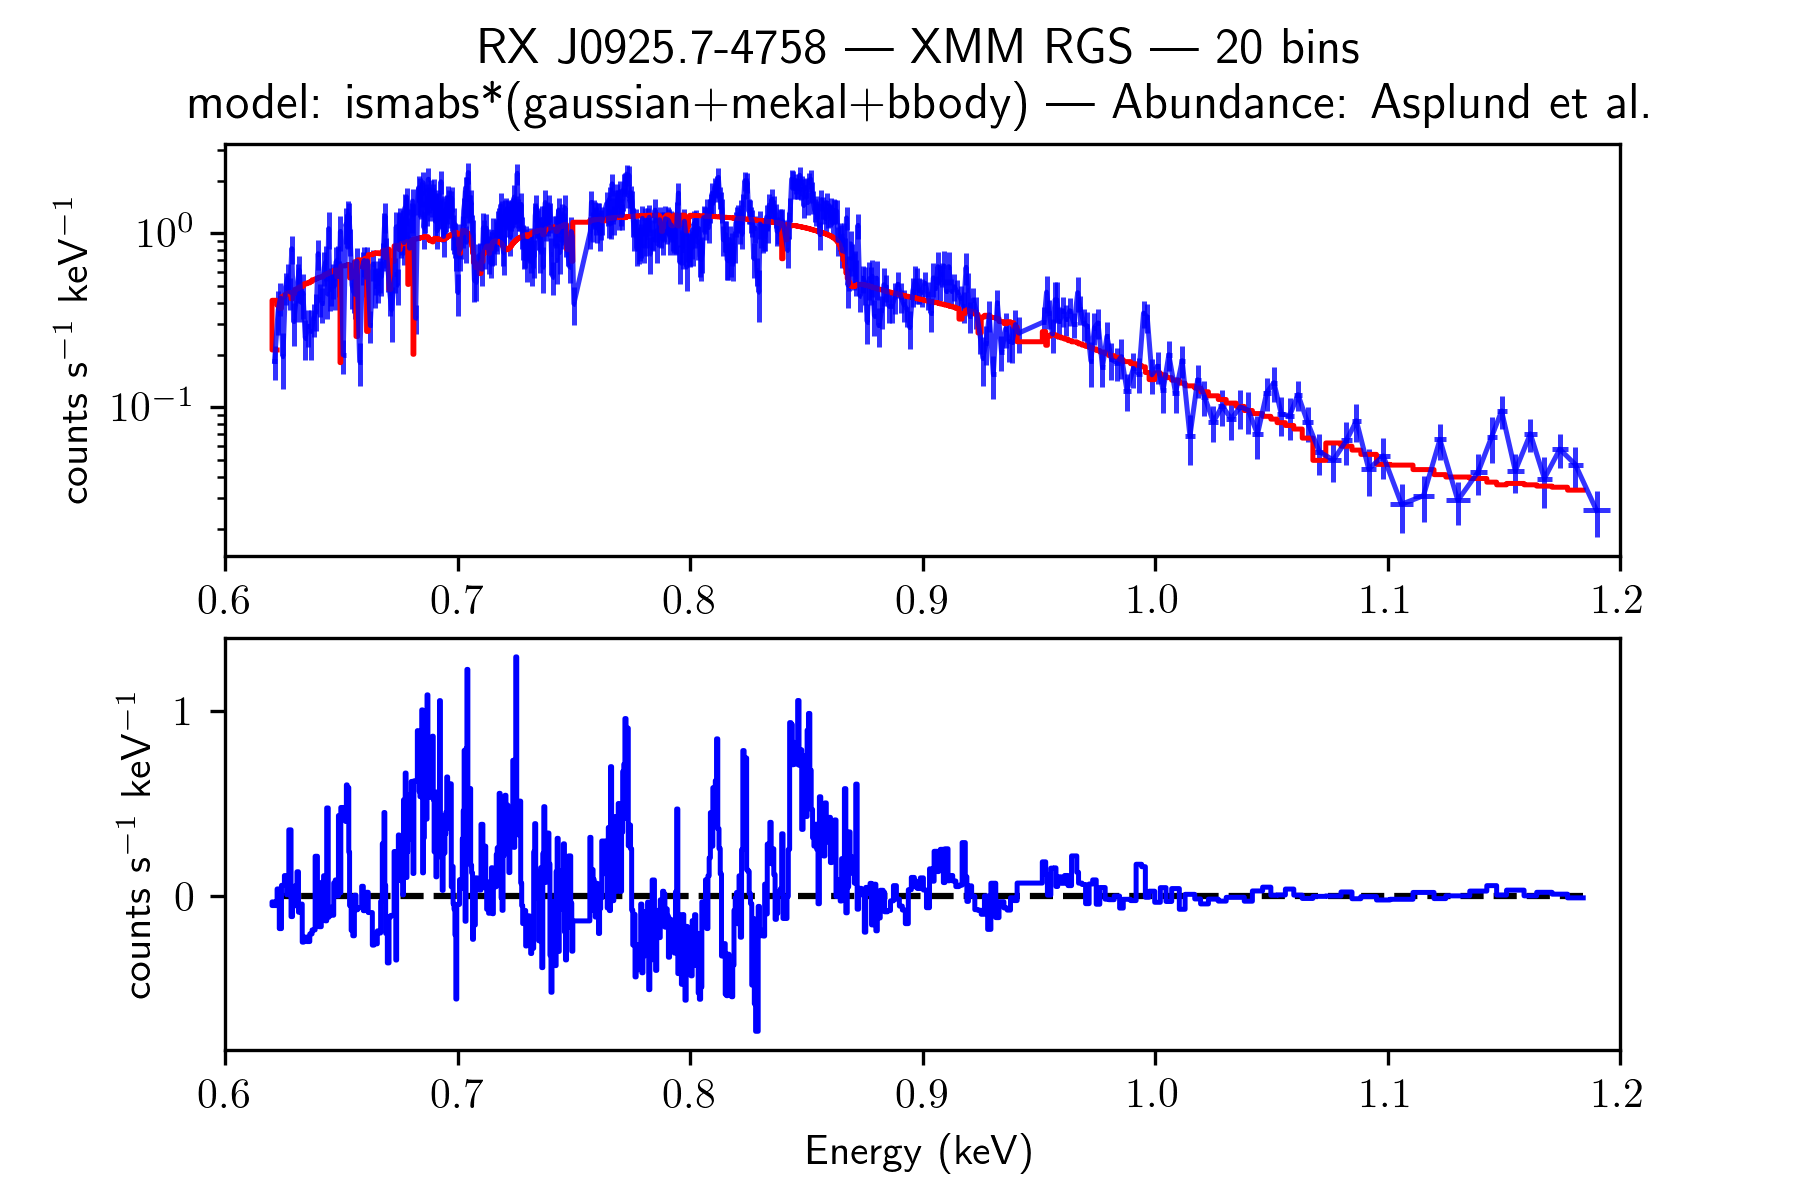
\includegraphics[width=0.45\textwidth]{mrvel-rgs2-o1-m07}} %\hfill
				\subfloat[Order 2 \label{xmm:rgs2-m07:o2}]{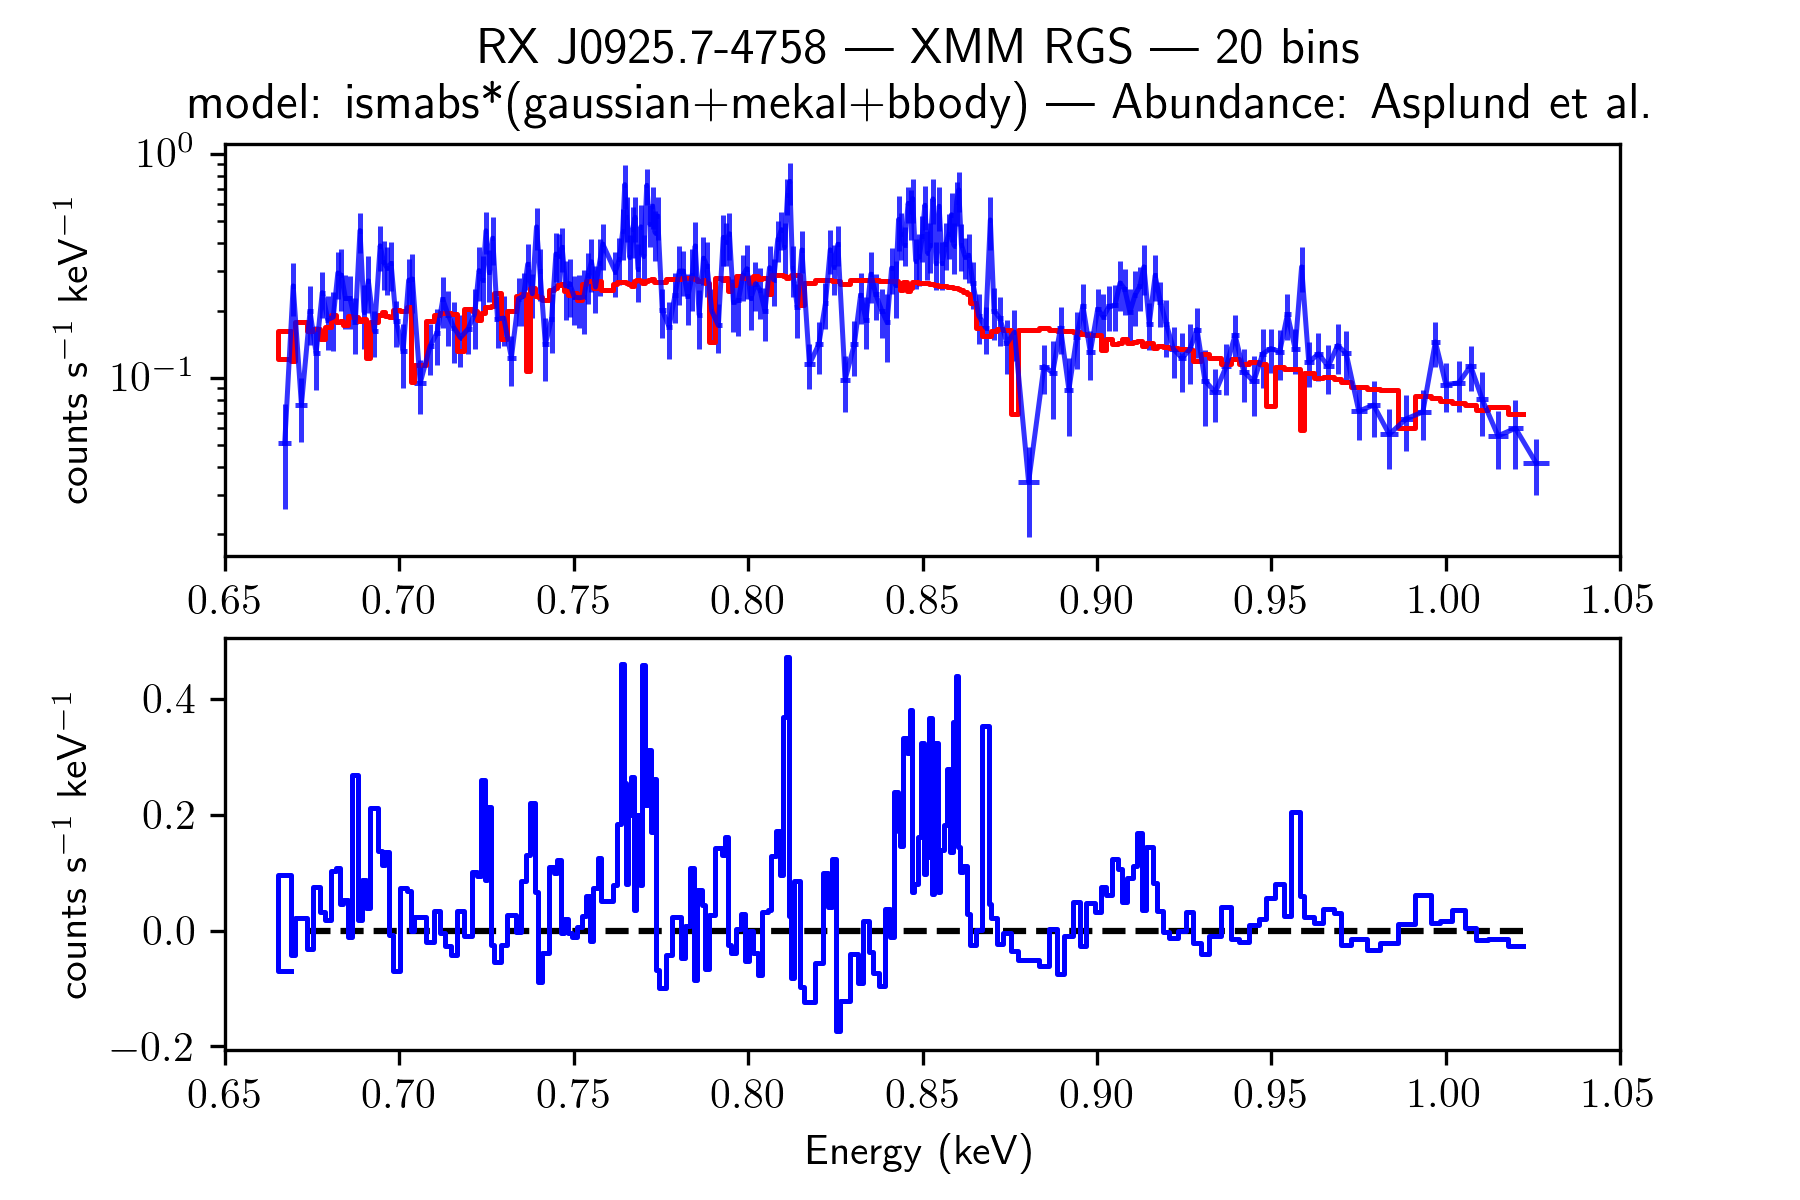
\includegraphics[width=0.45\textwidth]{mrvel-rgs2-o2-m07}} %\hfill
			\end{figure}
			\begin{figure}[h!]
				\centering
				\caption{Spectral fits for RGS2 spectra using model M08}
				\label{xmm:rgs2-m08}
				\subfloat[Order 1 \label{xmm:rgs2-m08:o1}]{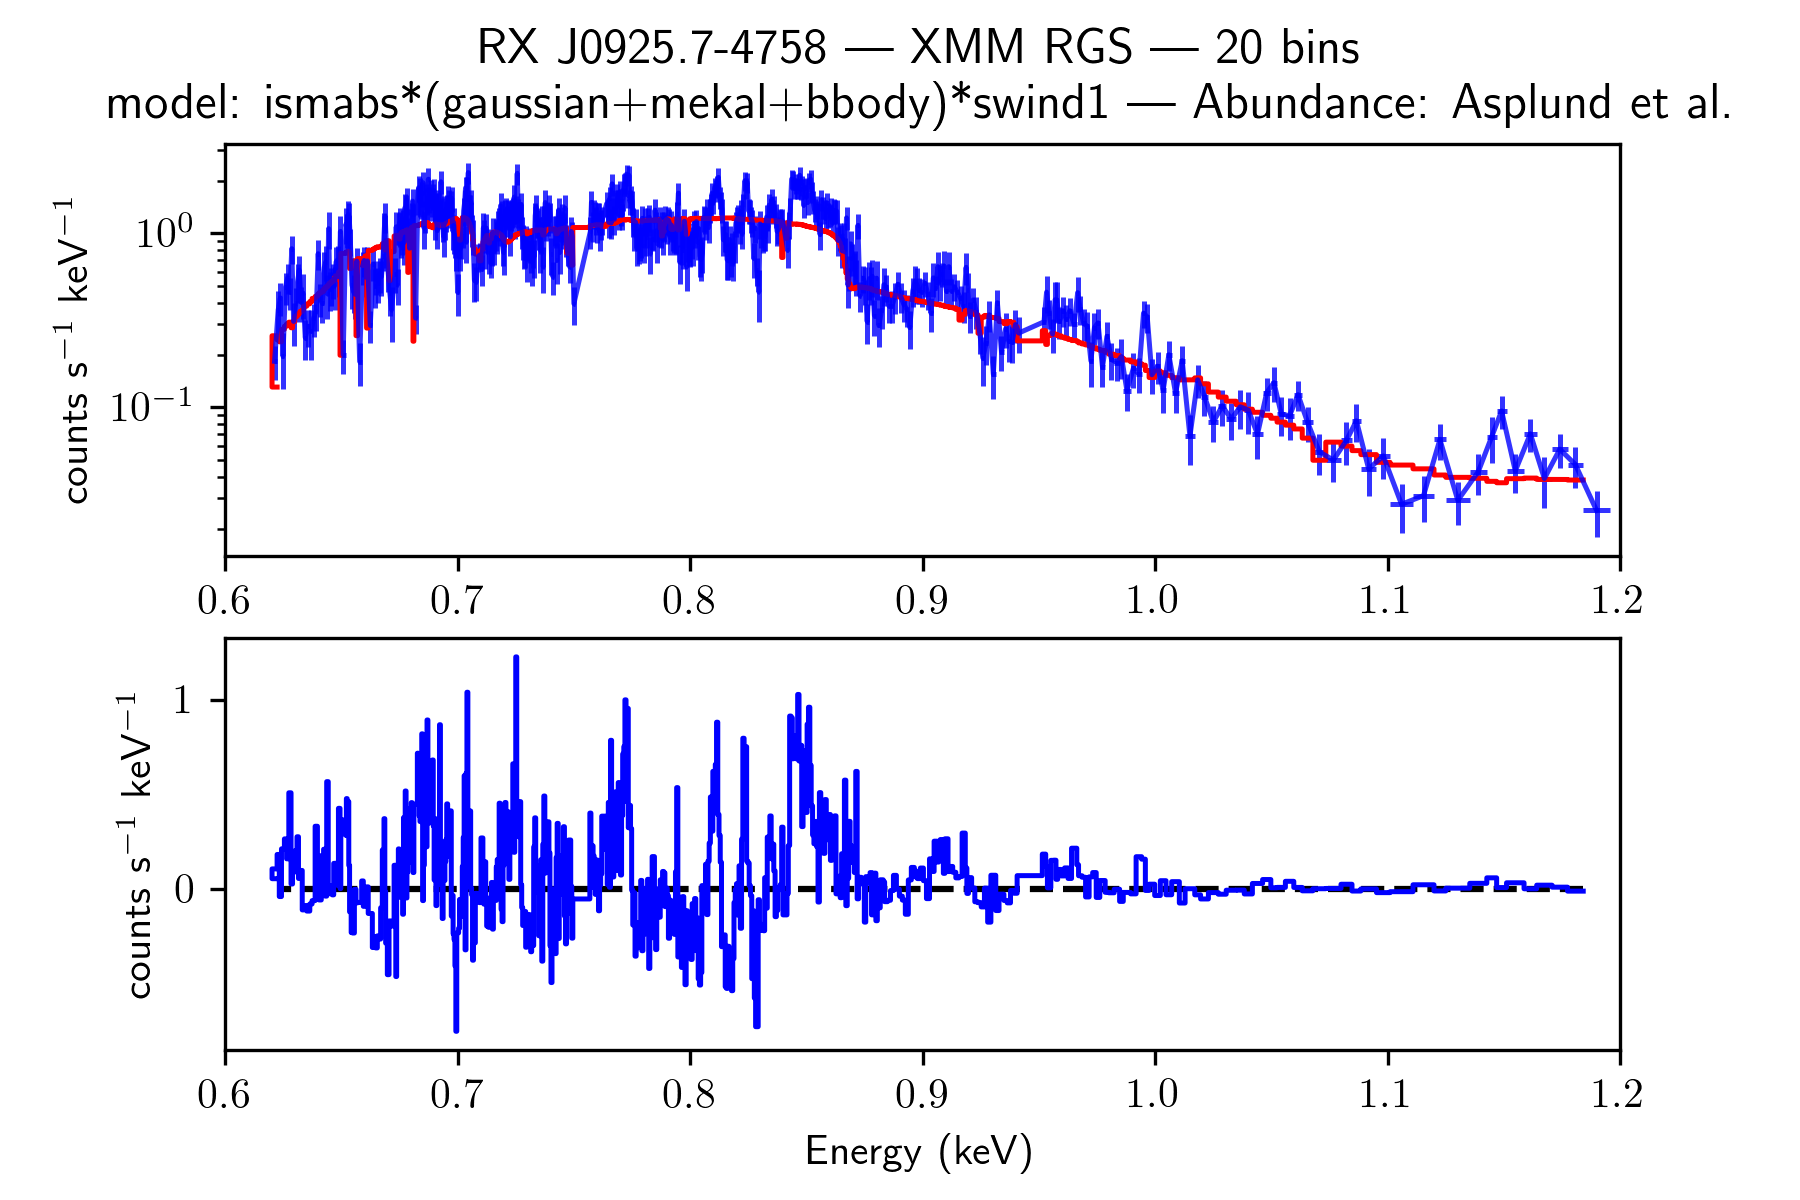
\includegraphics[width=0.45\textwidth]{mrvel-rgs2-o1-m08}} %\hfill
				\subfloat[Order 2 \label{xmm:rgs2-m08:o2}]{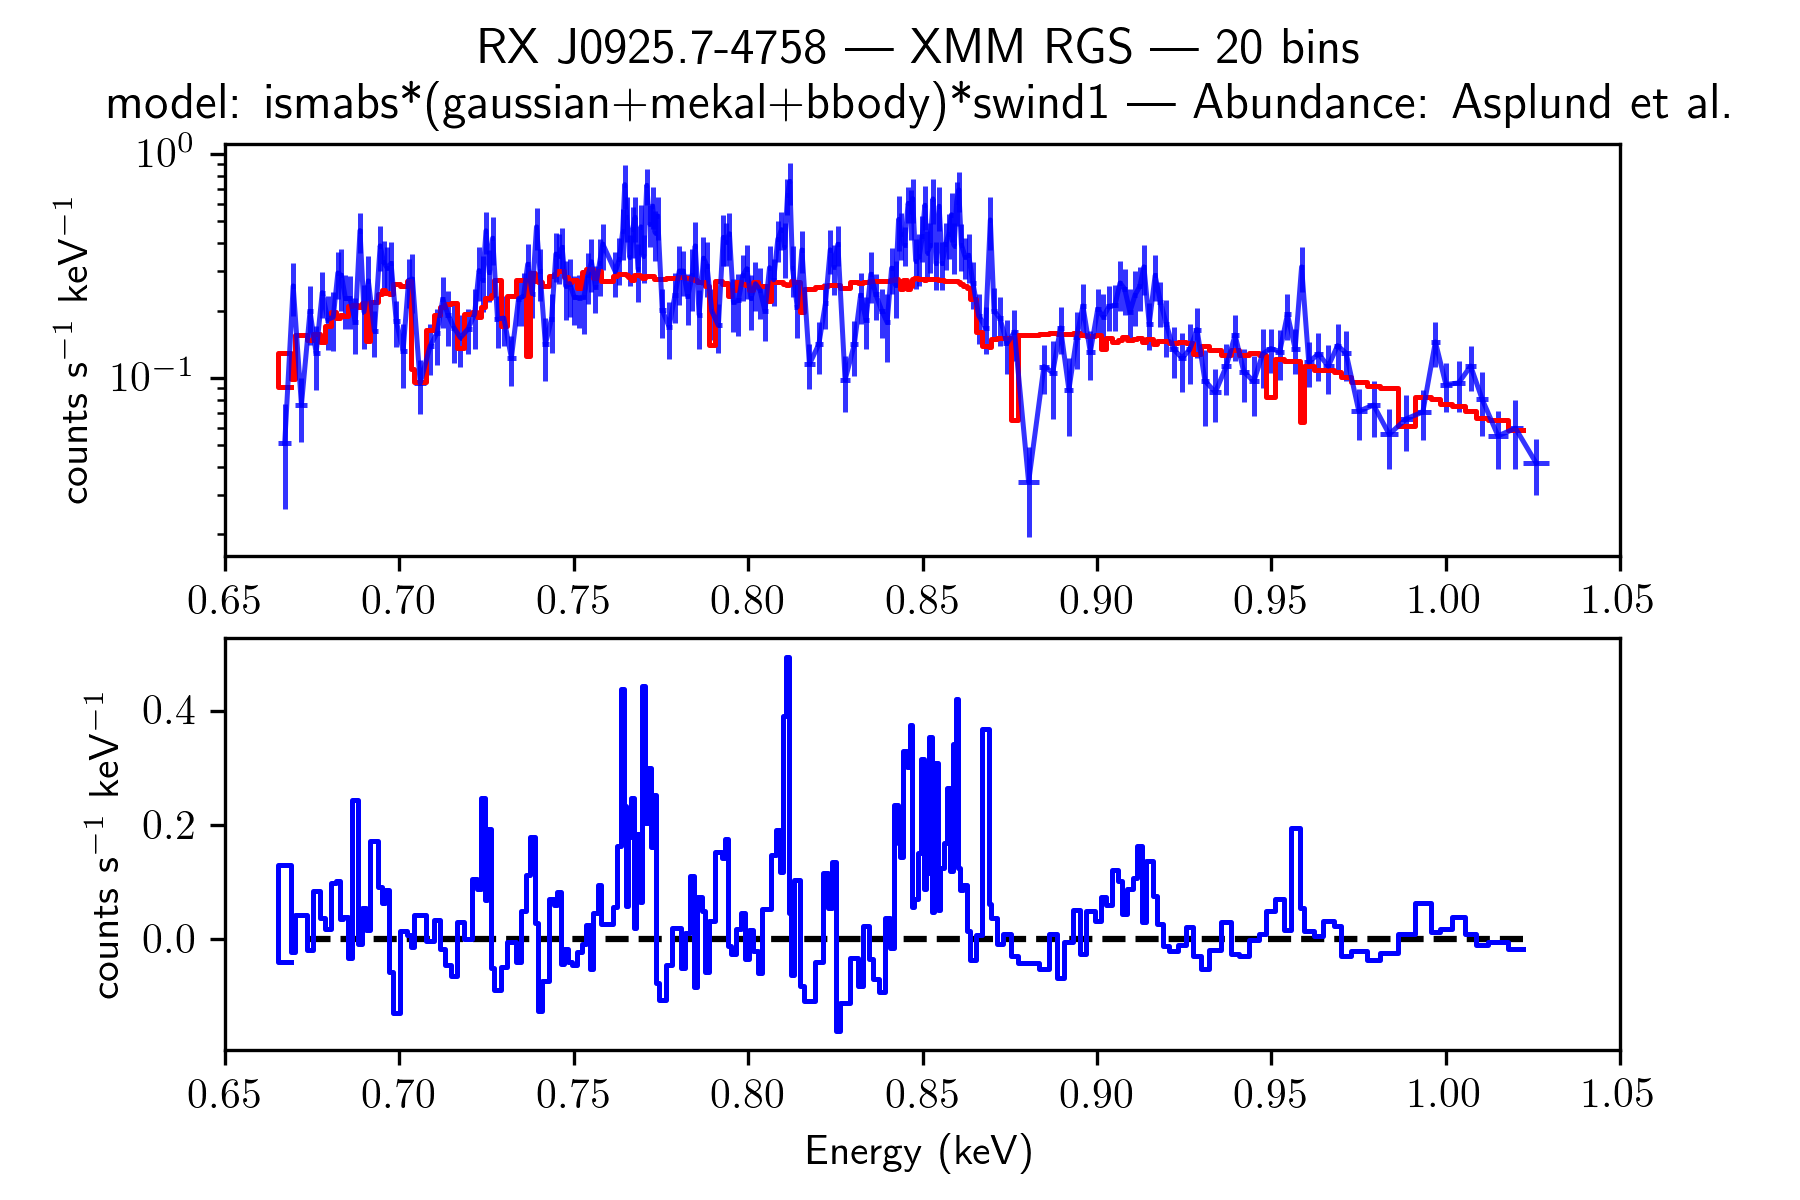
\includegraphics[width=0.45\textwidth]{mrvel-rgs2-o2-m08}} %\hfill
			\end{figure}
			\begin{figure}[h!]
				\centering
				\caption{Spectral fits for RGS2 spectra using model M09}
				\label{xmm:rgs2-m09}
				\subfloat[Order 1 \label{xmm:rgs2-m09:o1}]{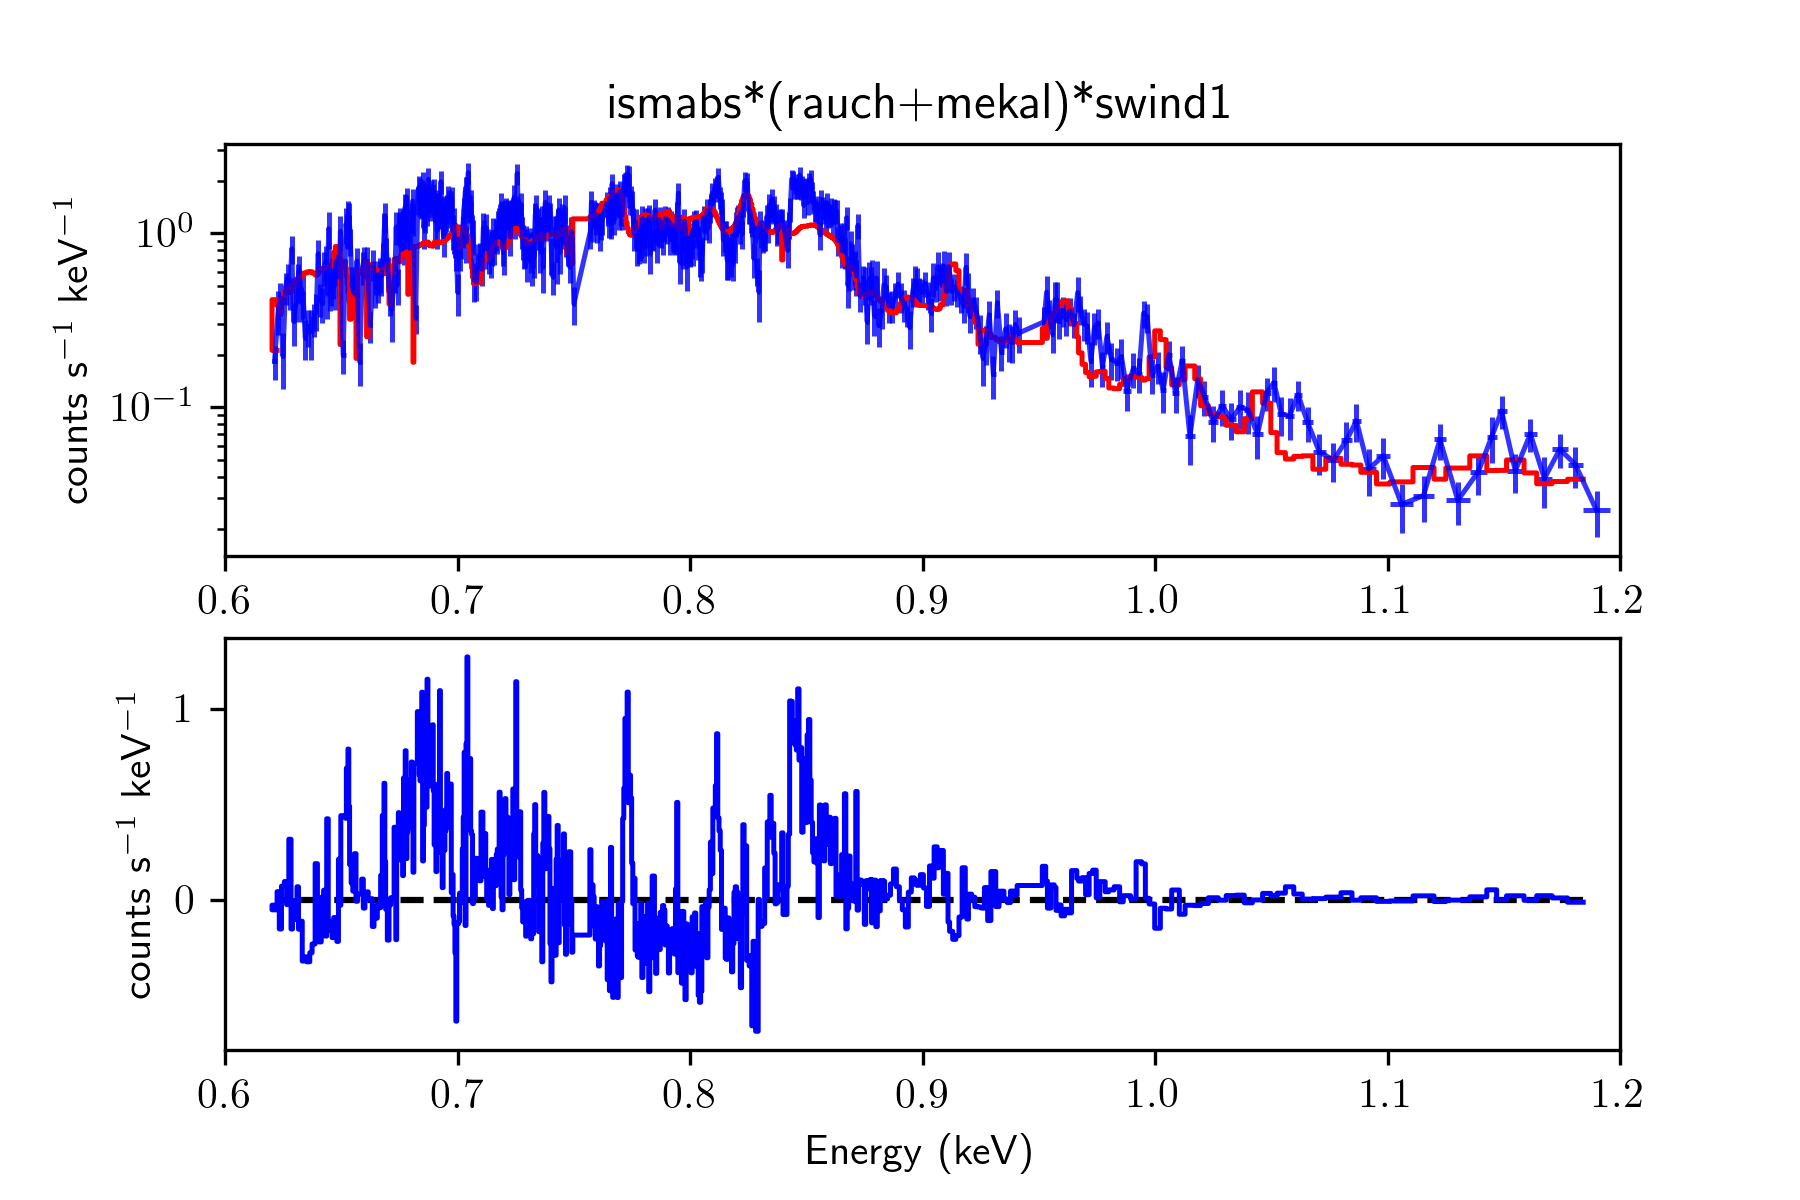
\includegraphics[width=0.45\textwidth]{mrvel-rgs2-o1-m09}} %\hfill
				\subfloat[Order 2 \label{xmm:rgs2-m09:o2}]{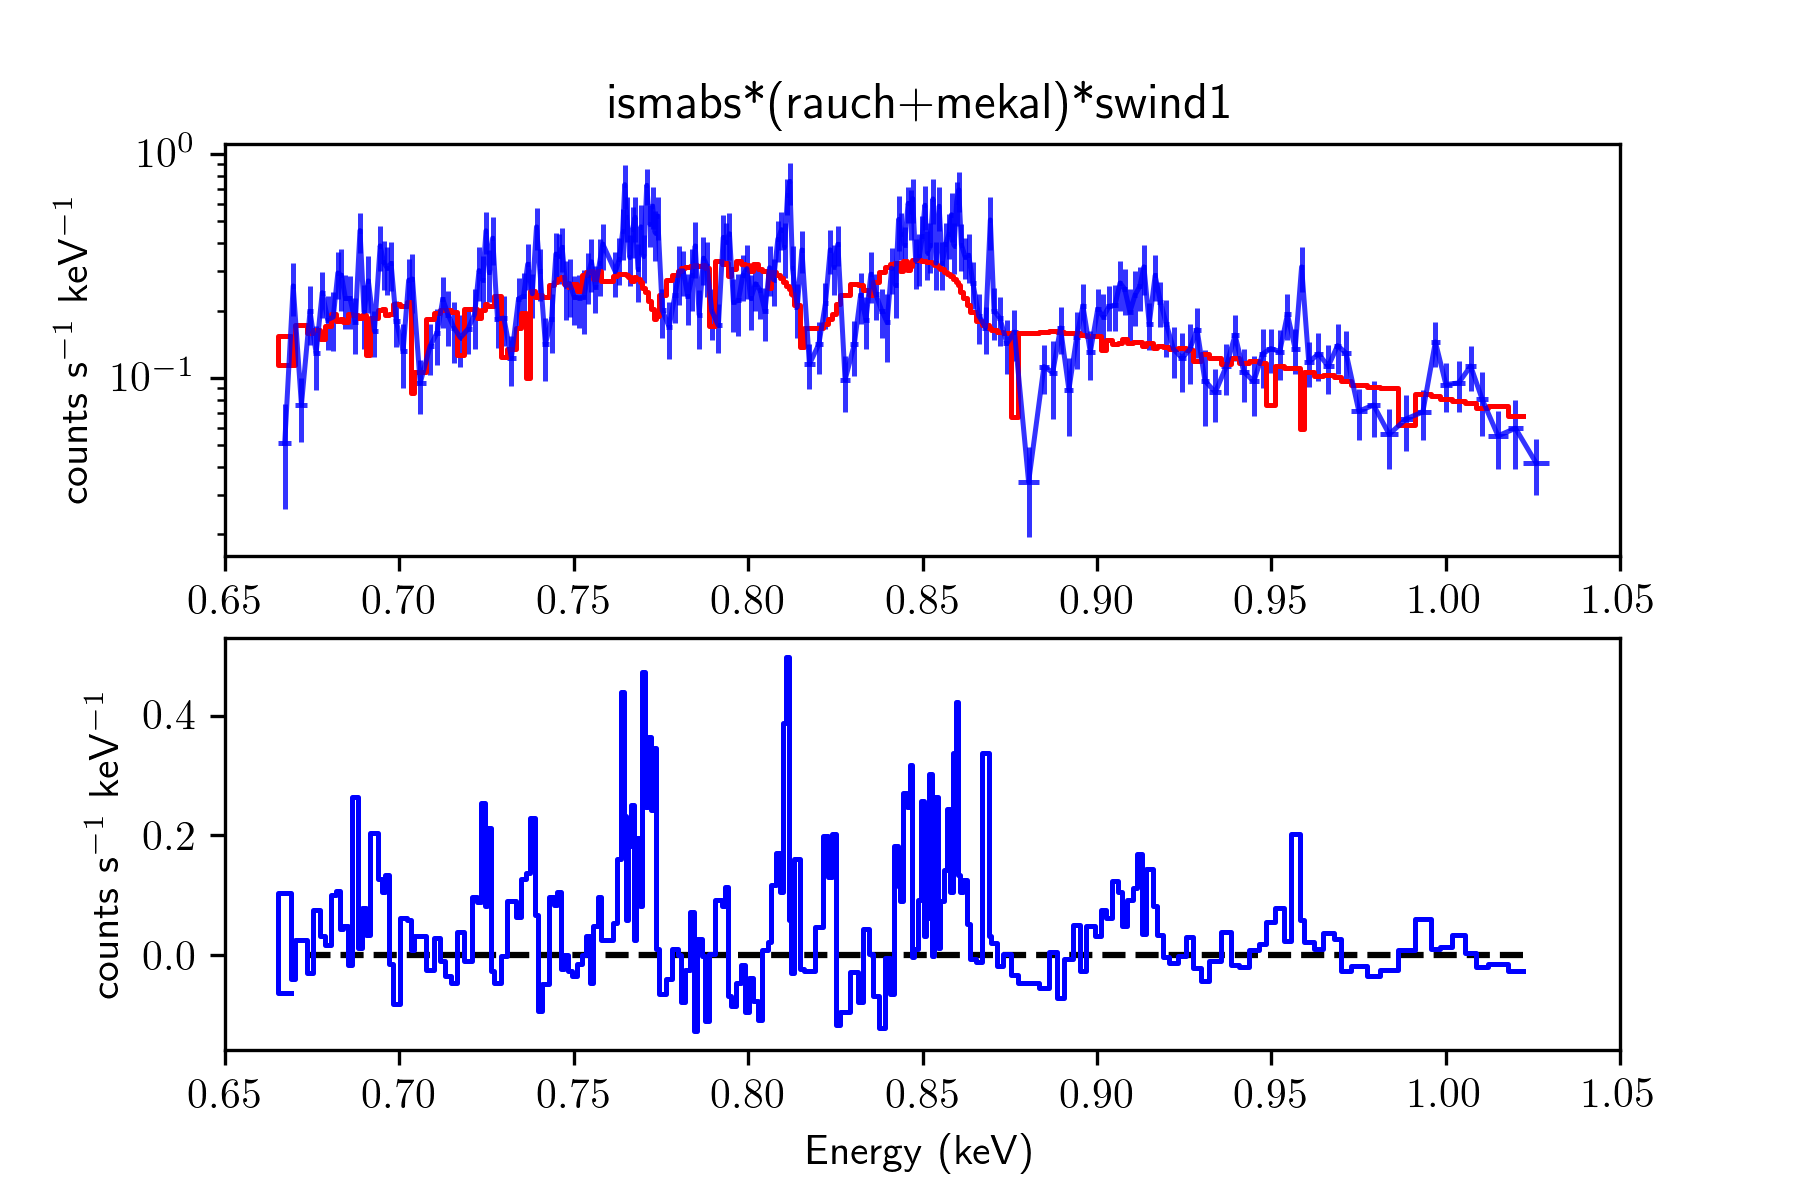
\includegraphics[width=0.45\textwidth]{mrvel-rgs2-o2-m09}} %\hfill
			\end{figure}
			\begin{figure}[h!]
				\centering
				\caption{Spectral fits for RGS2 spectra using model M10}
				\label{xmm:rgs2-m10}
				\subfloat[Order 1 \label{xmm:rgs2-m10:o1}]{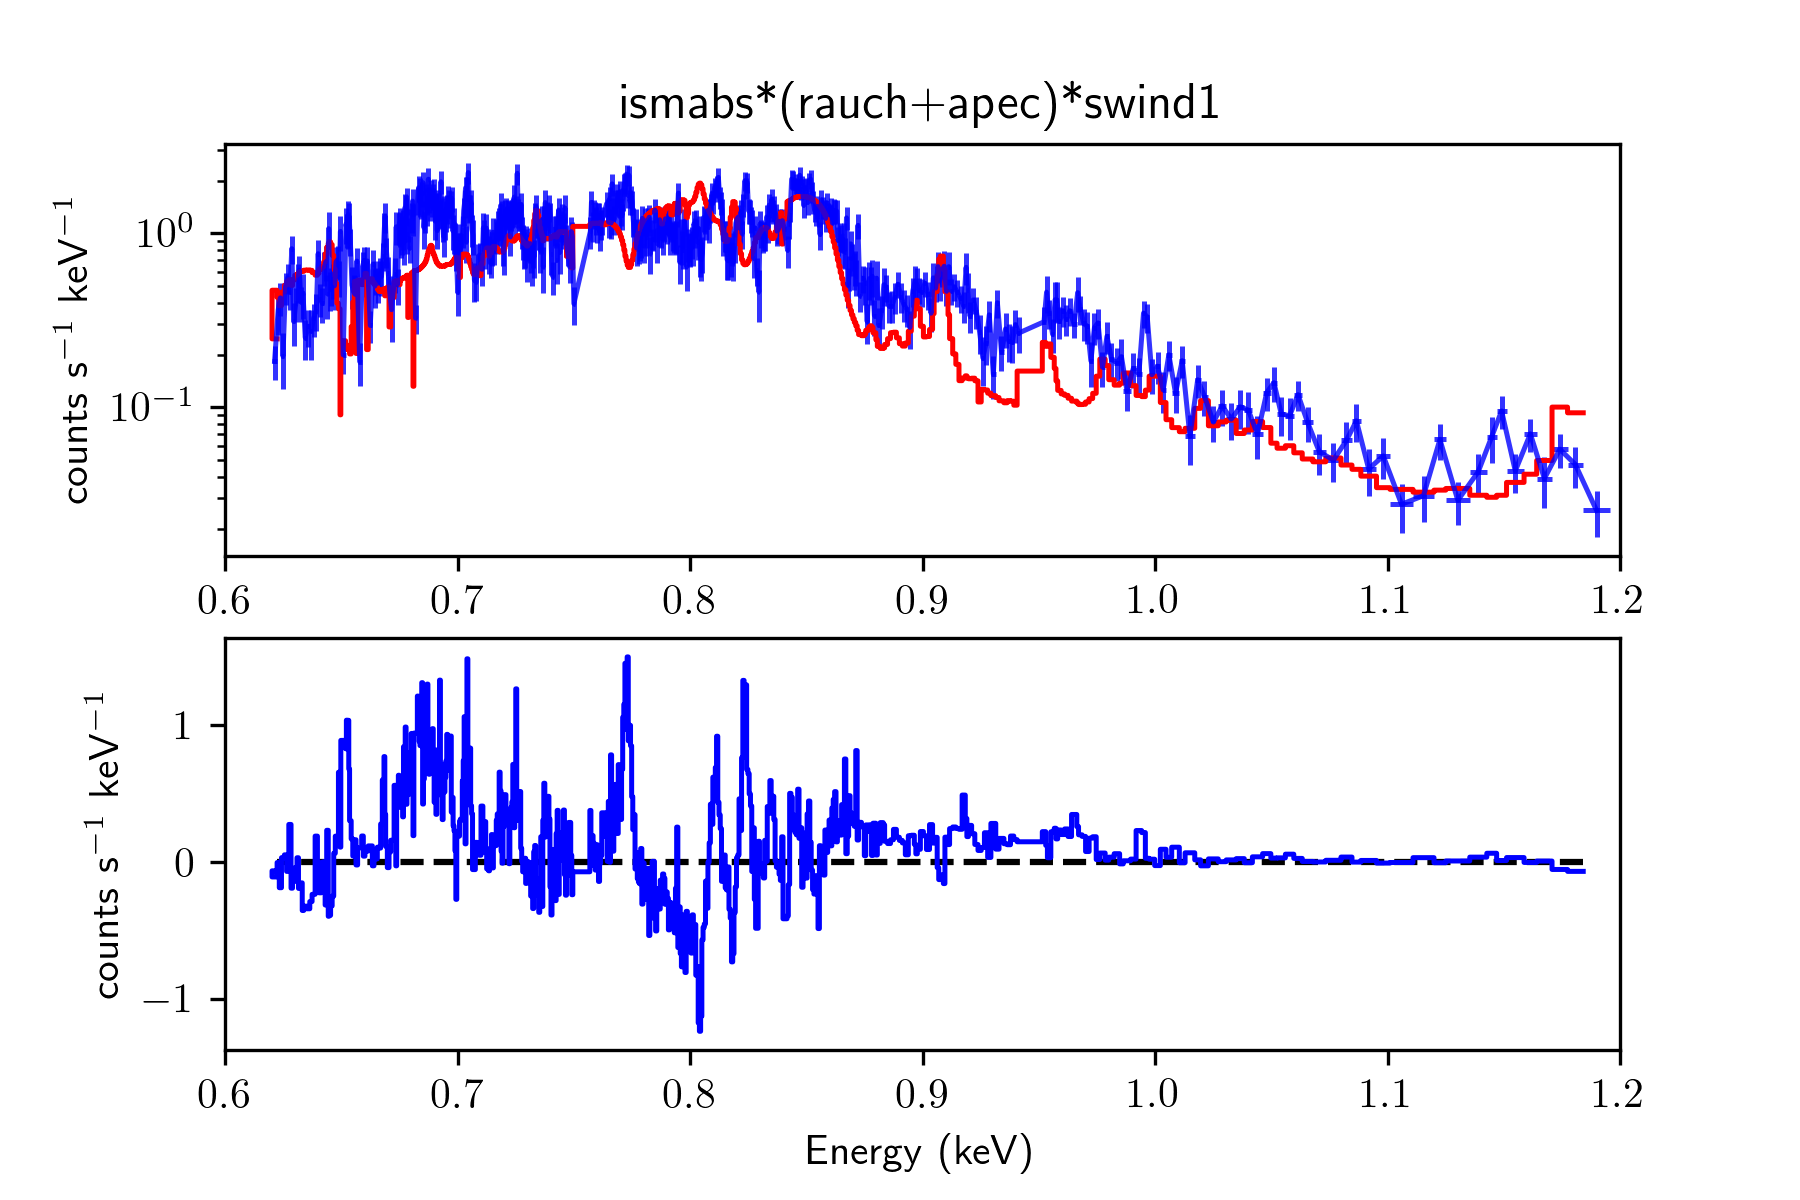
\includegraphics[width=0.45\textwidth]{mrvel-rgs2-o1-m10}} %\hfill
				\subfloat[Order 2 \label{xmm:rgs2-m10:o2}]{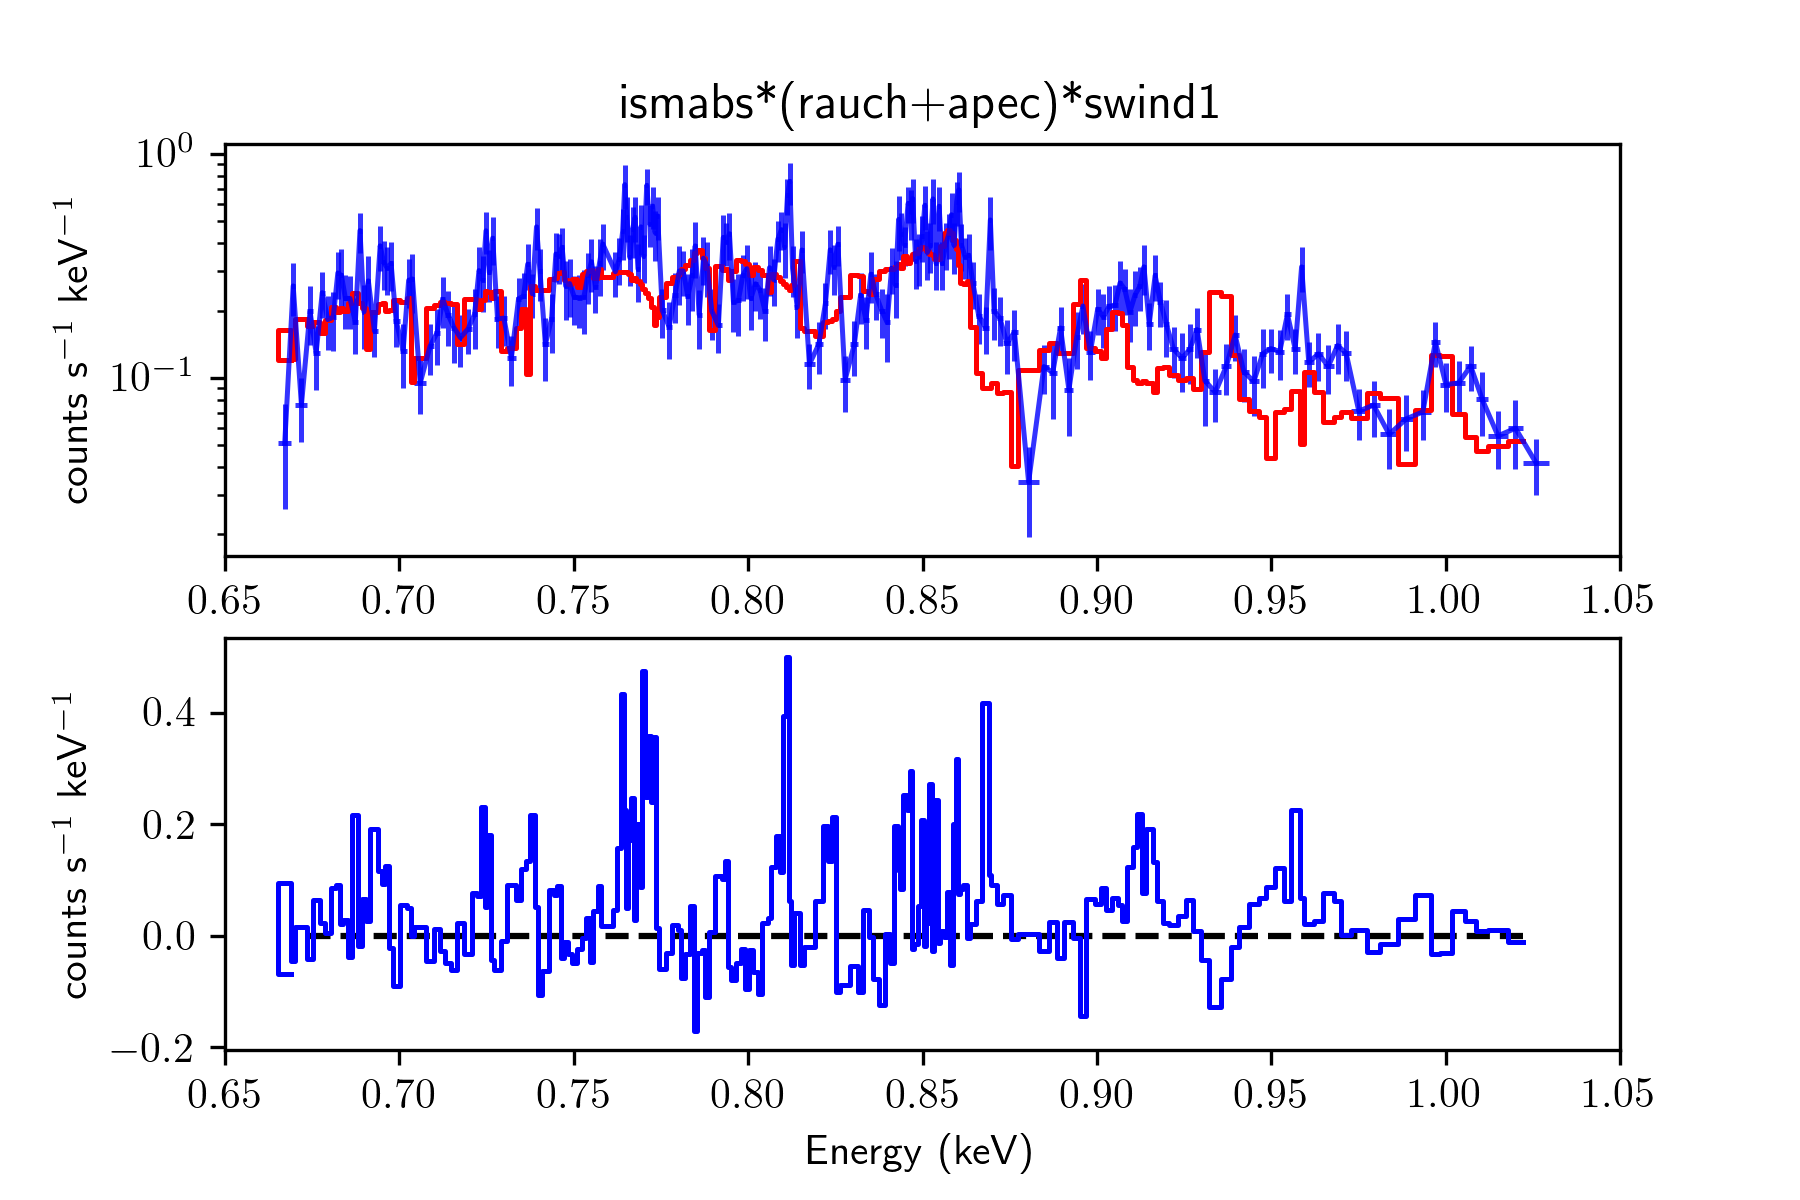
\includegraphics[width=0.45\textwidth]{mrvel-rgs2-o2-m10}} %\hfill
			\end{figure}
			\begin{figure}[h!]
				\centering
				\caption{Spectral fits for RGS2 spectra using model M11}
				\label{xmm:rgs2-m11}
				\subfloat[Order 1 \label{xmm:rgs2-m11:o1}]{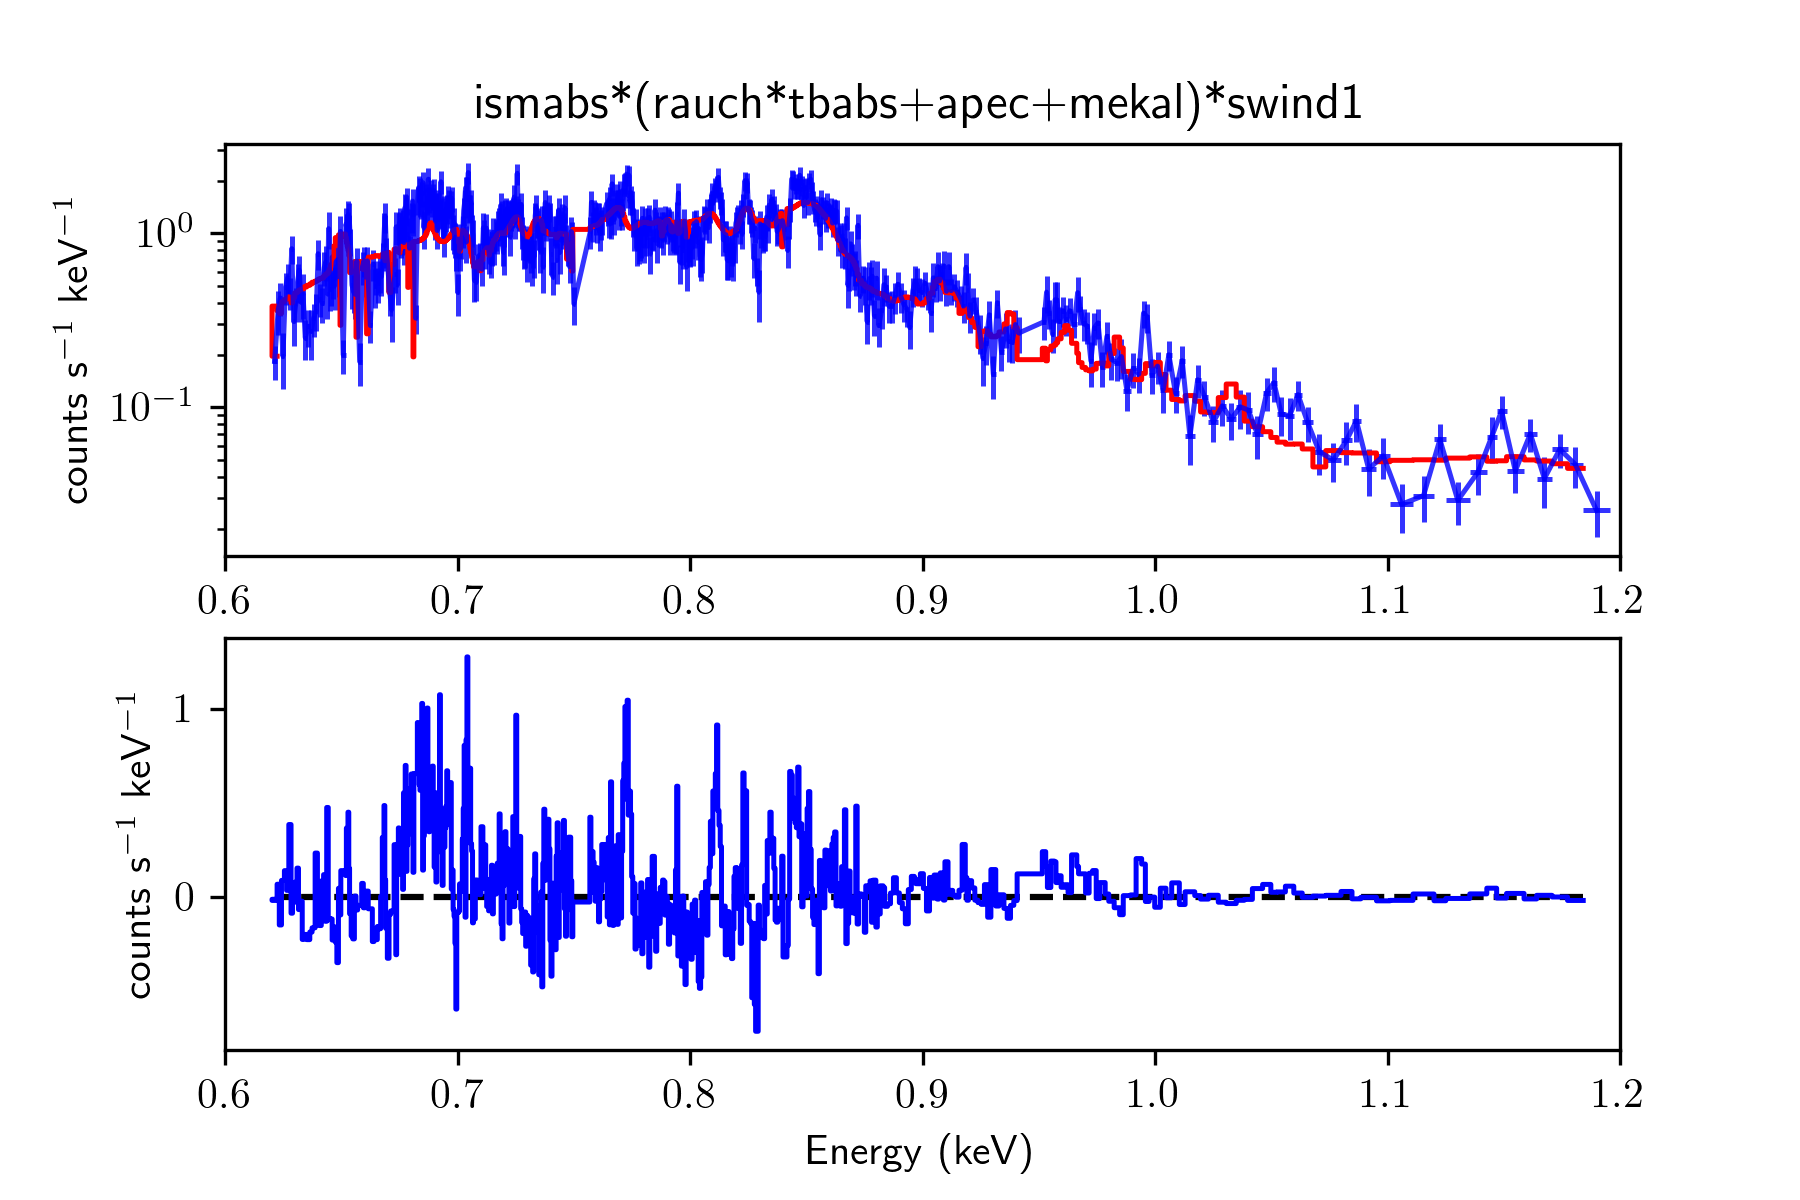
\includegraphics[width=0.45\textwidth]{mrvel-rgs2-o1-m11}} %\hfill
				\subfloat[Order 2 \label{xmm:rgs2-m11:o2}]{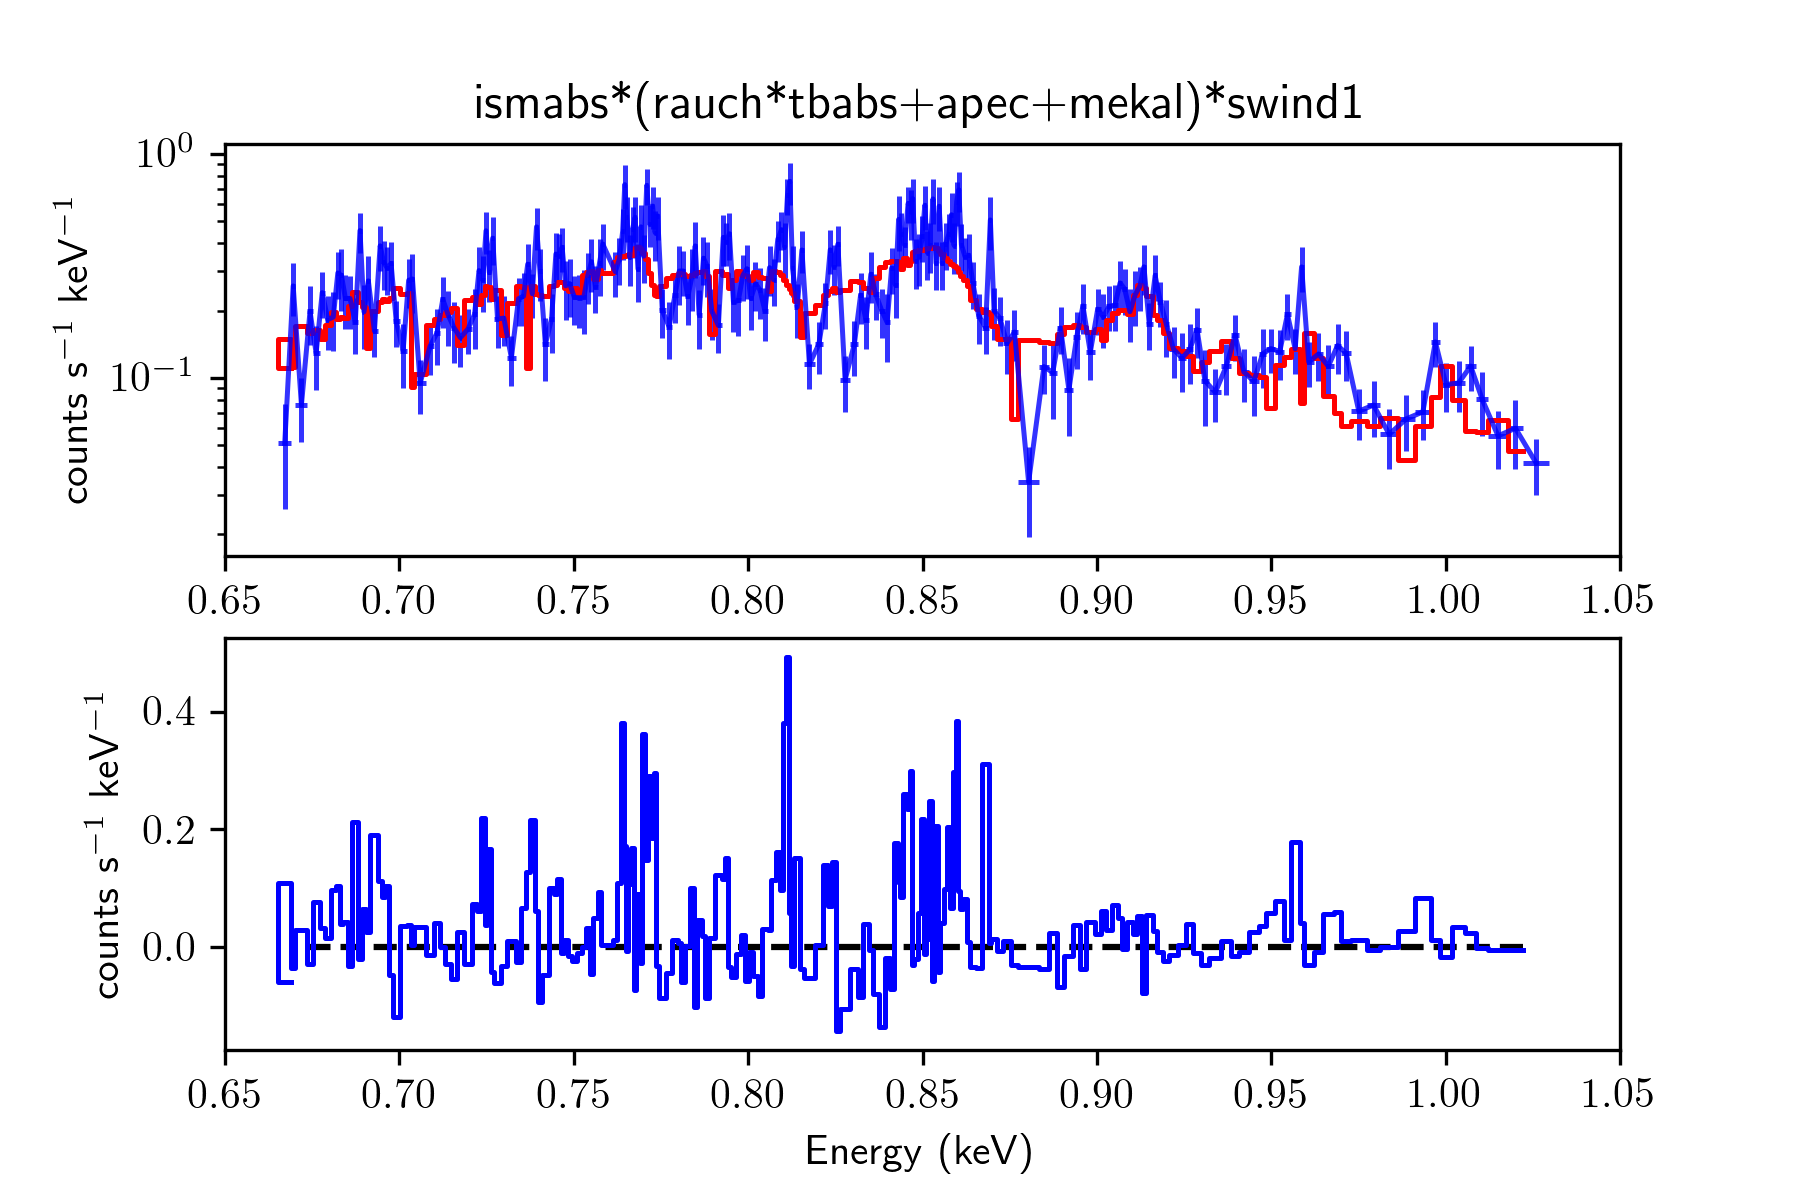
\includegraphics[width=0.45\textwidth]{mrvel-rgs2-o2-m11}} %\hfill
			\end{figure}
			\begin{figure}[h!]
				\centering
				\caption{Spectral fits for RGS2 spectra using model M12}
				\label{xmm:rgs2-m12}
				\subfloat[Order 1 \label{xmm:rgs2-m12:o1}]{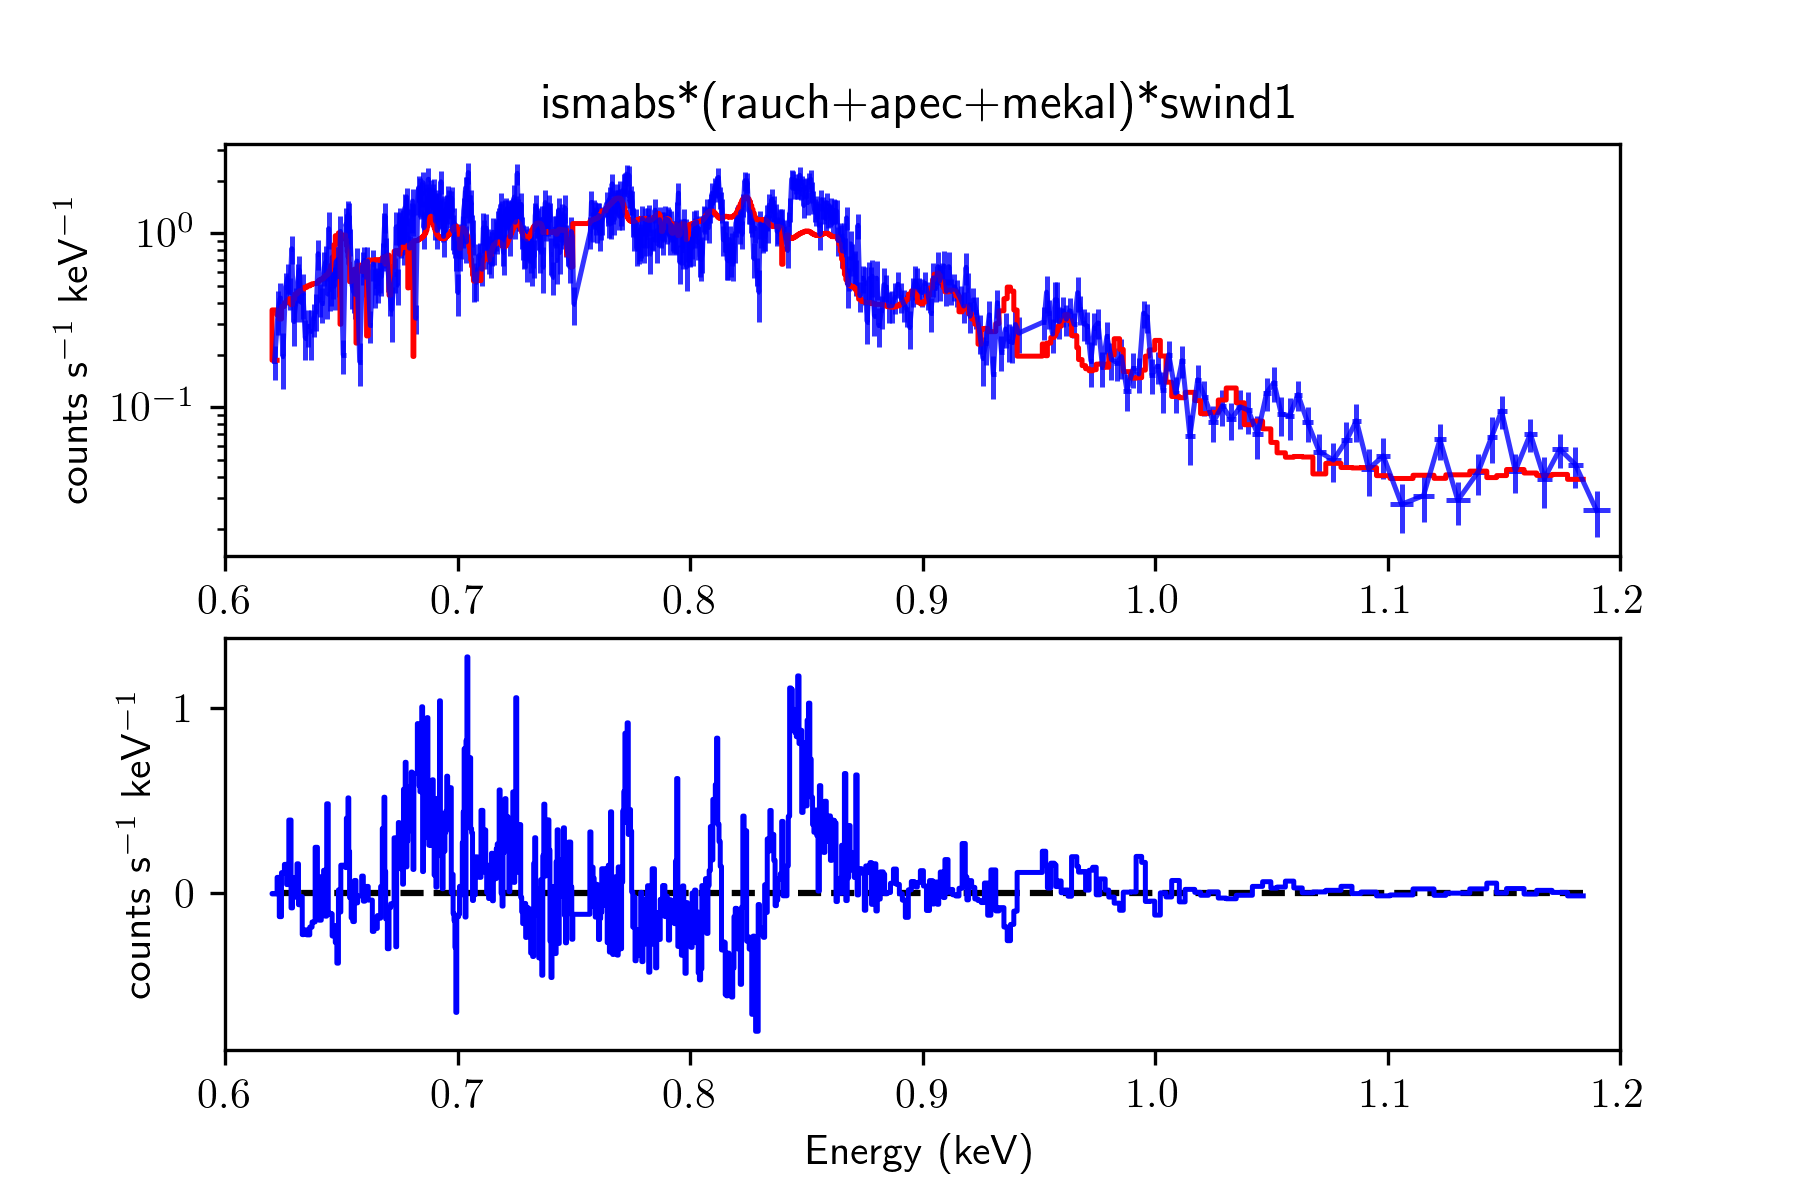
\includegraphics[width=0.45\textwidth]{mrvel-rgs2-o1-m12}} %\hfill
				\subfloat[Order 2 \label{xmm:rgs2-m12:o2}]{\includegraphics[width=0.45\textwidth]{mrvel-rgs2-o2-m12}} %\hfill
			\end{figure}
			
		%\subsection{With Order 1 Spectrum} \label{hi-resolution:analysis:order-1}
			%The 1$^{\mathrm{st}}$ order diffraction spectrum was fitted using the six models mentioned in \S\ref{hi-resolution:analysis} in the same order. The progression of the models increased the number of parameters, in spite of which there seems to be an improvement in the fit, as compared to those in available in literature. The best fit also seems to show significant abundances for NeI, MgI and ArI, at $2.87\times 10^{18}$, $1.10\times 10^{18}$ and $5.35\times 10^{18}$ respectively, as compared to the other metals included in the model.
			
			%\begin{figure}[h!]
			%	\centering
			%	\caption{Fitted spectrum using composite model}
			%	\subfloat[\texttt{ismabs*edge*edge*edge*(gaussian+bbody)} \label{xmm-rgs:01}]{\includegraphics[scale=0.45]{mr-vel-xmm-rgs-01.pdf}}
			%\end{figure}
			
			%But there are large deviations, especially for the softer X-ray photons. This is mainly because of the fact that the current model only incorporates continuum components. To fit the large number of observed lines in the spectrum, one needs to also include model components that account for emission lines. The additive model \texttt{mekal} computes an emission spectrum from hot diffuse optical plasma (perhaps a hot corona) based on the model calculations of Mewe, Kaastra and Liedahl. The \texttt{gaussian} component is replaced with \texttt{mekal} and an attempt was made to fit the same spectrum again.
			%\begin{figure}[h!]
			%	\centering
			%	\caption{Fitted spectrum using composite model}
			%	\subfloat[\texttt{ismabs*edge*edge*edge*(mekal+bbody)} \label{xmm-rgs:02}]{\includegraphics[scale=0.45]{mr-vel-xmm-rgs-02.pdf}}
			%\end{figure}
			
			%An improvement in the fit was observed, with a reduced $\chi^2$ value of 3.81. A visual inspection of the fitted spectrum shows that the softer photons have been accounted for with this model. This model also seems to show significant abundances for OI, NeI, MgI and SiI at $5.57\times 10^{18}$, $3.06\times 10^{18}$, $3.84\times 10^{19}$ and $7.02\times 10^{18}$ respectively.

		%\subsection{With Order 2 Spectrum} \label{hi-resolution:analysis:order-2}
			%The previous composite model was used to fit the 2$^{\mathrm{nd}}$ order diffraction spectrum, with a maximum grouping of 20 bins.
			
			%\begin{figure}[h!]
			%	\centering
			%	\caption{Fitted spectrum using composite model}
			%	\subfloat[\texttt{ismabs*edge*edge*edge*(mekal+bbody)} \label{xmm-rgs:03}]{\includegraphics[scale=0.45]{mr-vel-xmm-rgs-03.pdf}}
			%\end{figure}
			
			%This spectrum showed another improvement in the fit, which is reflected in the reduced $\chi^2$ value of 2.56. This fit shows the abundances for many species. NI, OI, NeI, MgI, SiI, ArI and Fe showing abundances of $1.06\times 10^{18}$, $4.61\times 10^{18}$, $1.67\times 10^{18}$, $3.61\times 10^{19}$, $5.54\times 10^{18}$, $5.20\times 10^{16}$ and $1.31\times 10^{17}$ respectively.
			
			%However, the soft X-ray photons seen in the 1$^{\mathrm{st}}$ order spectrum seems to be missing in the  2$^{\mathrm{nd}}$ order spectrum. A fluxed spectrum comprising of data from both diffraction orders could be constructed and subsequently analysed.
	% COMPLETE
    %\chapter{PARAMETERIZATION OF P CYGNI PROFILES DUE TO STELLAR WINDS} \label{chap:tool}
\chapter{TOOL FOR IDENTIFICATION OF SPECTRAL LINES IN XMM-NEWTON RGS SPECTRA} \label{chap:tool}
    %\doublespacing
    \minitoc
    \begin{center}
    	\emph{Abstract of chapter \ref{chap:tool}}
    \end{center}
    The identification of absorption and emission lines due to atomic species in the spectra of a X-ray binaries can reveal a wealth of information regarding the composition and physics of the stellar atmosphere. With the availability of high-resolution X-ray spectra from the RGS equipment on-board the XMM-Newton satellite, the study of such lines offers valuable diagnostics into the behaviour and evolution of the source object. Currently, data related to various atomic transitions, which lead to line formation, are made publicly available in the form of credible databases, one of them being the Atomic Spectra Database (ASD) at the National Institute of Standards and Technology (NIST). In this chapter, we present the development of a Python-based tool that accesses the relevant atomic data at NIST ASD for a given set of atomic species in a specific wavelength range and then overlays these lines on top of an X-ray spectrum obtained by the RGS spectrum of the XMM-Newton. With this tool, the astronomer can perform the important preliminary task of rudimentary line identification, before proceeding to advanced analysis of the X-ray data.
    
    \section{Introduction} \label{tool:intro}
    	XMM-Newton is an X-ray space observatory which was launched by the European Space Agency on December 10, 1999. It is designed to be a high throughput X-ray spectroscopy mission with spectral resolution of up to 0.025 \AA\ at 1 keV from the Reflection Grating Spectrometer (RGS) detectors and an angular resolution of up to 1.1 arcsec from the European Photon Imaging Cameras (EPIC) \cite{ehle2003xmm,jansen2001xmm}. With a bandpass of 5--38 \AA, corresponding to the energy range 0.33--2.5 keV, the spectra detected by RGS spans a substantial number of X-ray emission lines, which include the K-shell transitions and He-like triplets of light elements, such as C, N, O, Ne, Mg and Si, as well as the L-shell transitions of heavier elements like Fe and Ni. These factors enable the RGS spectra to be useful as diagnostic tools that can be used to investigate the physical conditions as well as the composition of the source of the spectra.
    
    \section{Working with RGS Data Files} \label{tool:rgs-files}
        The RGS spectra are available in the public domain in the \textit{Flexible Image Transport System} (FITS) file format \cite{chiappetti2018definition}, which is an open standard describing the digital file format for the storage, transmission and processing of data – formatted as multi-dimensional columns of tables. In spite of having the word `image' in its acronym, FITS files are most often used to store non-image data as well. This standard was designed, keeping in mind specifically astronomical data, namely images, spectra, lightcurves, photon lists, event lists, and source lists. In order to download the raw science data collected by XMM-Newton for any given source, there are two options:
        \begin{enumerate}[a)]
            \item By accessing the \textit{XMM-Newton Science Archive} (XSA) at the European Space Agency (ESA), using a web service (via a search form or a URL command access or methods from the \texttt{astroquery.esa.xmm\_newton} Python module) or by  \textit{table access protocol} (TAP) queries to the XSA database \cite{arviset2002xmm}.
            
            \item By accessing the \textit{High Energy Astrophysics Science Archive Research Center}, or HEASARC, at the National Aeronautics and Space Administration (NASA) using a web service \cite{barrett1993heasarc}.
        \end{enumerate}
        
        The XMM-Newton Science Operations Centre (SOC) provides a software package called the \textit{Science Analysis System} (SAS)\footnote{\url{https://www.cosmos.esa.int/web/xmm-newton/sas}}, which is a collection of tasks, scripts and libraries designed for the specific tasks of the reduction and analysis of the raw science data collected by the XMM-Newton observatory \cite{de2019users}. Using SAS, one can extract an RGS spectrum from the science data for a given X-ray source.
        
        An X-ray spectrum from RGS is found to contain a multitude of absorption and emission lines corresponding to atomic transitions in elements heavier than H and He. One of the initial and crucial tasks of the observer is to make a preliminary identification of the elemental lines at the wavelengths where they appear. This line identification also needs to incorporate the shift in the apparent position of the wavelength due to the Doppler effect. Currently, such line identification is performed by spectral-fitting programs such as Xspec or Spex while fitting the spectrum to prior theoretical models in which one can include the desired elemental abundances. However, when the spectrum used is of very high-resolution (such as that obtained from XMM-Newton), it often leads to poor fits, especially when one includes non-LTE model atmospheres. A Python-based tool was developed to address these deficiencies with the following motivation:
        \begin{enumerate}[a)]
            \item To upend the approach for fitting such high-resolution spectra by allowing the user to first quickly identify the prominent lines present in the spectrum as well the Doppler shift in the lines (if any).
            \item To estimate the elemental abundances (from the presence of specific lines) and the radial velocity of the emitting material (from the Doppler shifts).
            \item To allow the user to develop models for the individual lines and thereby engineer composite theoretical models which are more phenomenological as opposed to traditional approaches \cite{ness2020complications}.
        \end{enumerate}
        As present, while there are available codes that enable the parsing of atomic line data from NIST ASD (such as the \texttt{nist-asd} Python package on PyPI) or object-oriented interface for Xspec (i.e. PyXspec), there is a lack of tools or codes that allow \textit{a priori} identification of spectral lines identification.
        
        In order get started, one first needs to obtain data of the atomic lines from credible databases, such as the \textit{Atomic Spectra Database} (ASD)\footnote{\url{https://www.nist.gov/pml/atomic-spectra-database}} at the \textit{National Institute of Standards and Technology} (NIST)\footnote{\url{https://www.nist.gov/}} \cite{ralchenko2008nist} and \textit{The Opacity Project online atomic database} (TOPbase)\footnote{\url{https://cds.unistra.fr/topbase/topbase.html}} \cite{cunto1993topbase}. To obtain this data, one may either use the web service provided to send queries to these databases, or one may use the relevant methods in various Python modules.
        
        Having identified the prominent lines in the RGS spectrum, one can then proceed to estimate the radial velocity of the source, the abundance of the elements in the emitting material and the interstellar absorption along the line-of-sight.
        
        \subsection{Extraction of RGS Spectra} \label{tool:rgs-files:extraction}
        
            \subsubsection{Obtaining source-specific science data} \label{tool:rgs-files:extraction:data}
                XMM-Newton data is publicly available at the online multi-mission science data archive known as HEASARC (\url{https://heasarc.gsfc.nasa.gov/}). The easiest way to access relevant data for any specific source is by using its browse service at \url{https://heasarc.gsfc.nasa.gov/db-perl/W3Browse/w3browse.pl} where one can enter the name of the source (or its right ascension and declination, if these are known) and the mission name (such as XMM-Newton or Chandra). One can supply additional information about the source as well, such as the observation dates. The more specific the query, the lesser would be the time taken to access and download the data.
                
                HEASARC provides the relevant data products in the form of a \texttt{.tar} file, which may then be extracted to obtain the \textit{Observation Data Files} (ODF), in case of XMM-Newton.
            
            \subsubsection{Reprocessing of science data} \label{tool:rgs-files:extraction:reprocess}
                The downloaded ODF files are compressed in \texttt{.gz} format and need to be extracted before reprocessing them using the software package SAS. Two SAS commands are used during the reprocessing – \texttt{cifbuild} and \texttt{odfingest}. While the former produces an index file of all the calibration data relevant to the specific source under consideration, the latter creates a summary file of the ODF using the house-keeping data files and the calibration database \cite{de2019users}.
                
                Subsequently, the data from both RGS instruments for the first and second spectral orders is extracted using the SAS task \texttt{rgsproc}. In five processing stages, this task extracts the events, the angles, the filter events, the spectra, the response matrices and the lightcurves.
        
        \subsection{Accessing Spectral Data from FITS Files} \label{tool:rgs-files:access}
            One of the outputs of the \texttt{rgsproc} task are two fluxed spectra -- one for each spectral order. Each of these files contain the spectra fluxed from both the RGS instruments. One must bear in mind that these fluxed spectra are inherently just a qualitative summary of the data, and should not be used for quantitative analysis. However, in the current work, because the objective is to merely aid the user in the identification of atomic lines -- which could be a preliminary step before serious spectral modeling, these fluxed spectra are more than sufficient as input files.
            
            \subsubsection{The \texttt{astropy} Python module} \label{tool:rgs-files:access:astropy}
                The fluxed spectrum file is saved in the FITS format. So the appropriate way to read its contents and extract the data is by using \texttt{astropy} \cite{robitaille2013astropy}, which is an open-source and community-developed Python package providing various functionalities that are important to astronomical applications.
                
                The \texttt{astropy.io.fits} package provides the user with access to FITS files. One first reads the list of \textit{header data units} (HDU), which is the highest level component of a FITS file -- consisting of a header and a table (or data array). This can be done using the \texttt{astropy.io.fits.open()} function which takes the FITS filename as input and returns an object of the \texttt{HDUList} class -- a list-like collection of HDUs.
            
            \subsubsection{Reading spectral data from FITS file} \label{tool:rgs-files:access:io}
                One can access the individual HDUs in a FITS file using the array indexing syntax -- the first index pointing to the primary HDU by default. For instance, if the object returned by the \texttt{astropy.io.fits.open()} function is named \texttt{hdul}, then \texttt{hdul[0]} would be the primary HDU, \texttt{hdul[1]} the first extension HDU and so on.
                
                In case of the fluxed spectra from RGS, the FITS files contain a single extension HDU corresponding to the spectrum -- accessed using \texttt{hdul[1]}, which is a table containing 3600 rows and 3 columns. Then the data attribute of \texttt{hdul[1]} (or \texttt{hdul[1].data}) would return a \texttt{NumPy} numerical array containing the channels/wavelengths (in \AA), the flux and the errors (both in s$^{-1}$cm$^{-2}$\AA$^{-1}$). The fluxes and errors corresponding to all bad channels contain \texttt{NaN} values, which can be filtered using the \texttt{isnan()} function and set to zero.
        
        \subsection{Collecting Atomic Lines} \label{tool:rgs-files:line-collection}
            In order to be able to identify atomic lines in a spectrum, one needs to have a line list that contains information about the lines present within a given wavelength range for all the ion stages of the atoms under consideration. With tremendous improvement in computing power, the various online databases of atomic data provide more accurate and updated information that may be used to built better line lists.
            
            So a code for qualitative atomic line identification in a spectrum becomes more reliable if it is able to access the current atomic data available online. This work achieves this objective by retrieving data for atomic transitions directly from ASD at NIST during runtime. So it is important to have an internet connection available while running the code for the first time or when one modifies the list of ions considered. As long as one keeps running the code subsequently on the same terminal session, using an unaltered ion list, the code would proceed to use the atomic data which is cached locally and one may work offline in that case.
            
            \subsubsection{The astroquery Python module} \label{tool:rgs-files:line-collection:astroquery}
                Atomic data from NIST can be accessed using the \texttt{astroquery} module \cite{ginsburg2019astroquery}, which uses the Python requests package for making HTTP requests and utilizes the data parsing functionality of the \texttt{astropy} package. The NIST ASD can be sent query requests and data retrieved therefrom using the \texttt{astroquery.nist} module.
            
            \subsubsection{Reading atomic line data from NIST} \label{tool:rgs-files:line-collection:NIST}
                The \texttt{astroquery.nist.Nist.query()} function provides an easy way to send HTML requests to NIST ASD. This function takes, as inputs, the lower and upper wavelength values and the name of the ion to be considered. One can also make use of the \texttt{astropy.units.AA} attribute to convert the wavelength value to \AA units.
                
                This function returns an object of the \texttt{astropy.table.Table} class. Then individual table rows can be accessed by the indexing syntax. The elements of a row can be subsequently accessed using the corresponding column header as a dictionary key. For instance, if the object named \texttt{ion\_table} stores the output of the \texttt{query()} function, then one can access the Ritz wavelength on the 17$^\text{th}$ row as \texttt{ion\_table[16]['Ritz']}.
        
        \subsection{Demonstration} \label{tool:rgs-files:demonstration}
            What follows is a demonstration of the developed tool using the flux spectrum of the galactic luminous supersoft X-ray source RX J0925.7-4758, which was discovered in the Galactic Plane Survey of the ROSAT All-Sky Survey \cite{motch1994}. The specific observations were made during 16-17 December 2000 with the RGS exposures being carried out for a duration of 61.2 ks \cite{motch02} under the observation ID 0111150101. The ODF files were downloaded from HEASARC and RGS data were processed using the SAS task \texttt{rgsproc} under default settings.
            
            Because the objective of this work is to enable the identification of atomic lines for specfic ion stages present in the spectrum, the fluxed spectrum file named \texttt{P0111150101O BX000fluxed1000.FIT} (produced by \texttt{rgsproc}) is sufficient for the code to work. This specific file fluxes together the first-order spectra from both the RGS instruments. A copy of this file is provided with the distribution of the code for the user to reproduce the demonstrations that follow, as well as to try out variations of the run.
            
            Three specific Python scripts are provided with the distribution, whose outputs are presented in this work. A study of these scripts provides the user with an experience of how to use the methods developed in this work. All the scripts take, as the second command-line argument, the name of the file containing the fluxed spectrum. Briefly, these scripts perform the following tasks:
            
            \begin{enumerate}[i.]
                \item \texttt{line-overlaid-flux.py}: computes all the atomic lines within the wavelength range chosen and produces a plot of the fluxed spectrum with these lines overlaid.
                
                \item \texttt{flux-inspect.py}: allows the user to examine specific regions of interest, such as the vicinity of a known atomic line, within the chosen wavelength range.
                
                \item \texttt{line-shift.py}: displays the Doppler shifts in the Lyman $\alpha$, $\beta$, and $\gamma$ lines for the H-like and He-like C, N and O ions, as well as some common Fe ion lines.
            \end{enumerate}
        
            \subsubsection{Reading fluxed spectrum from FITS file} \label{tool:rgs-files:demonstration:read-flux}
                The use of the \texttt{astropy.io.fits} module is wrapped up in a method named \texttt{get\_flux}. This method takes a single argument, which is the name of the FITS file containing the fluxed spectrum -- in this case, the file named \texttt{P0111150101OBX000fluxed1000.FIT}. It returns the wavelengths (in \AA), the normalized flux and the error (both in s$^{-1}$cm$^{-2}$\AA$^{-1}$) in the form of three lists, which can be subsequently manipulated.
                
            \subsubsection{Preview of spectrum} \label{tool:rgs-files:demonstration:preview}
                When one is working with the spectrum of a new source, one may not be aware of the wavelength region which contains most of photon flux. Also, RGS spectra tend to have  a very low SNR in the small wavelengths up to $\sim$7 \AA. So, in order to help the user to ascertain a more pragmatic range, the function named \texttt{preview\_flux} quickly plots the entire spectrum. This method takes, as arguments, two lists -- the wavelengths in \AA~and the flux. The preview of the first-order fluxed RGS spectrum for RX J0925.7-4758 is shown in figure \ref{fig:spec-preview}.
                
                \begin{figure}[h!]
    				\centering
    				\caption{Preview of fluxed spectrum}
    				\label{fig:spec-preview}
    				\includegraphics[width=0.8\textwidth]{images/mrvel_preview}
			    \end{figure}
			    
			    As it can be seen from the preview in figure \ref{fig:spec-preview}, there seems to be plenty of information in the vicinity of 6 \AA. But this is not usable because it is just noise arising from the low effective area of the RGS instrument in the low wavelength region which severely limits the resolving power of the RGS instrument, as described in the XMM-Newton User Handbook \cite{xmmUserHandbook}. Also, the region above 26 \AA~has a very low SNR. Looking at the wavelength region between 10 \AA~and 26 \AA~one can clearly visualise a typical spectrum as expected from a luminous X-ray binary source with a good SNR. These wavelength limits are subsequently taken as inputs from the user by the method \texttt{get\_wave\_limits}.
			 
            \subsubsection{Line list within chosen wavelength range} \label{tool:rgs-files:demonstration:linelist}
                One needs the line list from the NIST database for the given list of ions within a chosen wavelength range. To achieve this, a method called \texttt{get\_lines()} is provided. This takes, as input arguments, the lower and upper wavelength values (in \AA). It uses the list of ions provided in the file \texttt{ion.list}, which is accessed by the script using the \texttt{ASTRODAT} environment variable. Then it queries the NIST database using the \texttt{astroquery.nist.Nist.query()} method.
                
                The \texttt{get\_lines()} method  returns a list of dictionaries, with each dictionary containing four entries: the wavelength (in \AA), the associated ion, a boolean flag which indicates whether that line needs to be included and the colour with which the line is to be plotted. The colour of a line for a specific ion is obtained from another method called \texttt{get\_colour()}. This method uses a pre-defined dictionary of colour maps, from which a colour for a particular ion stage is sampled with the help of a \texttt{NumPy} array. One may add more colour maps corresponding to other ions which may not be included in the code at present.
                
                This method has two more default arguments that allow the user to provide a Doppler shift and to filter out ground level transitions. These arguments are as follows:
                
                \begin{enumerate}[i.]
                    \item An argument \texttt{v\_radial} to provide a radial velocity $v_\text{rad}$ (in km/s), which is then used to compute the Doppler-shifted position $\lambda$ of the line at $\lambda_0$ as
                    \begin{equation}
                        \lambda=\left( 1+\dfrac{v_\text{rad}}{c} \right)\lambda_0 \label{eqn-doppler-shift}
                    \end{equation}
                    The default value of this argument is 0.
                    
                    \item A flag named \texttt{ground\_transitions\_only} which ensures that only those lines are considered which are a consequence of transitions into/from the ground level of the individual ion. The default value of this argument is \texttt{True}, which greatly reduces the density of lines being taken into account.
                \end{enumerate}
            
            \subsubsection{Line-overlaid spectrum} \label{tool:rgs-files:demonstration:lineoverlay}
                Having read the FITS file containing the fluxed spectrum and queried the line list from NIST, one can then proceed to produce a plot of the spectrum, along with the lines overlaid on it. This can be done using the \texttt{plot\_spectrum()} method. This method takes, as input arguments, the lists containing the wavelengths, the fluxes, the errors in the flux, the line list and the lower and upper limits of wavelength.
                
                \begin{figure}[h!]
    				\centering
    				\caption{Line-overlaid spectrum -- output of \texttt{plot\_spectrum()} method}
    				\label{fig:line-overlay}
    				\includegraphics[width=\textwidth]{images/mrvel_line-overlay}
			    \end{figure}
                
                This method produces a set of three subplots: a plot of the spectrum only, a map of the lines within the wavelength region and a plot of the spectrum with the pertinent lines overlaid. The output of this code for the fluxed spectrum of RX J0925.7-4758 is shown in figure \ref{fig:line-overlay}. As expected, one can observe a profusion of spectral lines due to K-shell transitions of N and O, and due to L-shell transitions of the heavier element Fe. Such an overlay of spectral lines provides a grid of markers of prominent lines. But the actual presence of any line in the spectrum may be latched on to after a closer inspection of sub-regions, \textbf{as described in the following sub-section}.
                
                Prior to running the \texttt{plot\_spectrum()} method, one may also choose to display the wavelength values (in \AA) along with the ion label, using the boolean flag \texttt{show\_wavelen- gth} input argument, whose default value is \texttt{False}. One may also choose to normalize the fluxed spectrum to the range $[0, 1]$ in s$^{-1}$cm$^{-2}$\AA$^{-1}$ using the method \texttt{normalize()}, which takes a list of floats as input and returns another list of floats normalized appropriately. This is helpful in comparing the relative strengths of different lines.
            
            \subsubsection{Inspecting regions of interest} \label{tool:rgs-files:demonstration:roi}
                While the previous method described produces the entire spectrum with overlaid lines, it can be more helpful if one could precisely zoom into any specific region of interest, say between 16.5 \AA~and 18.4 \AA. This can be done with the \texttt{examine\_ROI()} method, which takes the lists of wavelengths, fluxes and errors, the line list, the chosen wavelength range and the lower and upper wavelengths (in \AA) of the region of interest (e.g. 16.5 and 18.4).
                
                \begin{figure}[h!]
    				\centering
    				\caption{Partitioning of the fluxed spectrum within specific regions of interest}
    				\label{fig:roi}
    				\includegraphics[width=\textwidth]{images/mrvel_rois}
			    \end{figure}
                
                Such an inspection of specific regions of interest was carried out for RX J0925.7-4758 and the resulting plots are shown in figure \ref{fig:roi}. One can observe here, for instance, two lines (one due to Fe XVII and the other due to O VIII) nearly overlapping with an emission line in the spectrum around 16.03  \AA. Further analysis of the flux of other lines due to both atomic species would resolve this ambiguity.
                
            \subsubsection{Doppler shifts of lines} \label{tool:rgs-files:demonstration:doppler}
                The emitting matter in stellar sources often have a radial velocity along the line-of-sight because of which their atomic lines often exhibit a Doppler shift, which translates the lines either blue-ward (i.e. towards smaller wavelengths) if the radial velocity is negative (moving towards the observer) or red-ward (i.e. towards larger wavelengths) if the radial velocity is positive (moving away from the observer).
                
                This shift in the wavelength of a line can be obtained as
                
                \begin{equation}
                    \Delta\lambda=\lambda-\lambda_0 \label{eqn-doppler-02}
                \end{equation}
                
                where $\lambda_0$ is the central wavelength of the line and $\lambda$ is the apparent position of the same line. The relation between these two is given by equation \ref{eqn-doppler-shift}. By measuring the $\Delta\lambda$ value from the spectrum for some prominent and well-known atomic lines, one can estimate the radial velocity of the stellar matter which has produced the given spectrum.
                
                One can make an initial estimate of the Doppler shift by plotting the vicinity of a specific line by transforming the horizontal  axis from $\lambda$ (in \AA) to  (in km/s). Then $v_\text{rad}$ is obtained by inverting equation \ref{eqn-doppler-shift} as
                
                \begin{equation}
                    v_\text{rad}=\left( \dfrac{c}{\lambda_0} \right)(\lambda-\lambda_0) \label{eqn-vrad}
                \end{equation}
                
                A method named \texttt{waveshift\_to\_velocity()} is defined which returns $v_\text{rad}$ in km/s, given $\lambda_0$ and $\lambda$ in \AA~as input arguments.
                
                The method named \texttt{plot\_doppler\_lines()} can be used to plot the relative flux of different lines for a specific ion with respect to $v_\text{rad}$. At present, this method can handle the Lyman $\alpha$, $\beta$, and $\gamma$ lines for the H-like and He-like C, N and O ions, as well as some common lines of Fe XVII and Fe XVIII.
                
                The list of these lines is given in table \ref{tab:line-list}.
                
                \begin{table}[h!]
                    \centering
                    \caption{List of lines along with transitions, considered for inspection with respect to the radial velocity}
                    \label{tab:line-list}
                    \begin{tabular}{ccc}
                        \hline
                        \textbf{Ion} & \textbf{Transition} & \textbf{Wavelength (in \AA)} \\ \hline
                        \multirow{3}{*}{C V}      & {Ly $\alpha$} & {40.2678} \\ %\cline{2-3} 
                                                  & {Ly $\beta$}  & {34.9728} \\ %\cline{2-3} 
                                                  & {Ly $\gamma$} & {33.4262} \\ \hline
                        \multirow{3}{*}{C VI}     & {Ly $\alpha$} & {33.7396} \\ %\cline{2-3} 
                                                  & {Ly $\beta$}  & {28.4663} \\ %\cline{2-3} 
                                                  & {Ly $\gamma$} & {26.9901} \\ \hline
                        \multirow{3}{*}{N VI}     & {Ly $\alpha$} & {28.7870} \\ %\cline{2-3} 
                                                  & {Ly $\beta$}  & {24.8980} \\ %\cline{2-3} 
                                                  & {Ly $\gamma$} & {23.7710} \\ \hline
                        \multirow{3}{*}{N VII}    & {Ly $\alpha$} & {24.7846} \\ %\cline{2-3} 
                                                  & {Ly $\beta$}  & {20.9106} \\ %\cline{2-3} 
                                                  & {Ly $\gamma$} & {19.8261} \\ \hline
                        \multirow{3}{*}{O VII}    & {Ly $\alpha$} & {21.6020} \\ %\cline{2-3} 
                                                  & {Ly $\beta$}  & {18.6270} \\ %\cline{2-3} 
                                                  & {Ly $\gamma$} & {17.7680*} \\ \hline
                        \multirow{3}{*}{O VIII}   & {Ly $\alpha$} & {18.9725} \\ %\cline{2-3} 
                                                  & {Ly $\beta$}  & {16.0067} \\ %\cline{2-3} 
                                                  & {Ly $\gamma$} & {15.1765} \\ \hline
                        \multirow{3}{*}{Fe XVII}  & {2s$^2$2p$^6$ $\longrightarrow$ 2s$^2$2p$^5$3d} & {15.2620} \\ %\cline{2-3} 
                                                  & {2s$^2$2p$^6$ $\longrightarrow$ 2s$^2$2p$^5$(2P$^o_{3/2}$)3s} & {17.0510} \\ %\cline{2-3} 
                                                  & {2s$^2$2p$^6$ $\longrightarrow$ 2s$^2$2p$^5$(2P$^o_{1/2}$)3s} & {16.7760} \\ \hline
                        \multirow{3}{*}{Fe XVIII} & {2s$^2$2p$^5$ $\longrightarrow$ 2s$^2$2p$^4$(1D)3d} & {14.2080} \\ %\cline{2-3} 
                                                  & {2s$^2$2p$^5$ $\longrightarrow$ 2s$^2$2p$^4$(3P)3d} & {14.3730*} \\ %\cline{2-3} 
                                                  & {2s$^2$2p$^5$ $\longrightarrow$ 2s$^2$2p$^4$(3P)3s} & {16.0050*} \\ \hline
                    \end{tabular}
                \end{table}
                
                Another method named \texttt{map\_spec\_to\_vel()} maps the $\lambda$ values to the  values in the vicinity of a particular line using the previously described methods. It takes as input arguments the central wavelength of the line $\lambda_0$, the lists containing the wavelengths, fluxes and errors, and an argument called \texttt{v\_lim} which defines the bounds of $v_\text{rad}$ values, the default value of which is $\pm$5000 km/s.
                
                Finally, the method named \texttt{plot\_doppler\_lines()} wraps all of these and plots the line profiles for all the lines given in table \ref{tab:line-list}. In case of RX J0925.7-4758, no lines of C V and C VI and also for N VI were detected within the chosen wavelength range. Shown in the following figures are the line profiles obtained for the N VII, O and Fe ions. The \texttt{plot\_doppler\_lines()} method takes, as input arguments, the symbol of the element (`C', `N', `O' or `Fe'), the list of wavelengths, fluxes and errors and the symmetric bound of the radial velocity about 0 (which corresponds to the line centre).
                
                It also takes another argument named mode which serves to draw a dotted vertical line marker either through the lowest flux or the highest flux or both (within the range of radial velocities considered). Either of these options may be chosen by setting \texttt{mode=`abs'} (default value) or \texttt{mode=`ems'} respectively. One can also set \texttt{mode=`Pcyg'} to display both the markers simultaneously. However, one must be cautious while drawing any conclusions about the true position of the line centre from these markers because its position is merely ascertained from the flux values and are meant only to aid the user to get started with an approximate indication about the nature of the shift. For a more accurate evaluation, one needs to rely on a detailed quantitative analysis of the spectrum by using theoretical models.
    
    \section{Stellar Winds from Hot Luminous Massive Stars} \label{tool:stellar-winds}
        Hot luminous massive stars are those with effective temperatures $\sim 10000-50000$ K (i.e. spectral type A0 - O2), luminosities $\sim 10^{37}-10^{39}$ erg/s and masses $\sim 10-50$ M$_\odot$. At the end of their lifetime, such star could collapse as supernovae. If $F$ is the energy flux received at the telescope and $E$ is the energy radiated by the star, knowing the luminosity of such a star one can then use the ratio $\dfrac{F}{E}$ to determine their distances. This enables us to estimate the distances of the galaxies which the stars belong to.
        
        All hot stars with mass $\gtrsim 15$ M$_\odot$ show a high velocity outflow\cite{kudritzki2000winds}. Such an outflow is known as a stellar wind. Consequently, this leads to a mass loss from the star and the winds attaining a terminal velocity owing to Newton's first law of motion. Before proceeding further in the understanding of the driving mechanisms for stellar winds, one needs to be clear of these two important aspects.
        
        \subsection{Mass-Loss Rate} \label{tool:stellar-winds:mass-loss}
        	Due to the outflow of stellar material, the star suffers a mass loss, which is quantified by its \emph{mass-loss rate} $\dot{M}=\dvt{M}{t}$. Typical mass-loss rates of hot stars lie in the range $10^{-7}-10^{-4}$ M$_\odot$/yr, or approximately $\dfrac{1}{30}-30$ M$_\text{earth}$/yr. In comparison, the sun also has a mass outflow, called \emph{solar wind}, with $\dot{M}\approx 10^{-14}$ M$_\odot$/yr.
        
        \subsection{Terminal Velocity} \label{tool:stellar-winds:term-vel}
        	When stellar material is far from the surface of the star, it reaches its maximum velocity owing to the acceleration from the radiation pressure. At such large distances, due to the absence of any other external forces, the stellar velocity remains constant as per Newton's first law of motion. Therefore, this constant maximum velocity is known as the terminal velocity $v_\infty$.
        	
        	Typical values for $v_\infty$ lie between $\sim 200$ km/s (for A-type supergiants) and $\sim 3000$ km/s (for early O-type stars). Consequently, the speed of sounds in such atmospheres varies between 10 km/s to 30 km/s as per the relation:
        	\begin{align*}
        		V(R)=v_\infty\left(1-b\dfrac{R_*}{R}\right)^\beta
        	\end{align*}
	
	\section{Relevance of Stellar Winds} \label{tool:relevance}
		The analysis of stellar winds gains importance due to the reasons outlined below:
		\begin{itemize}
			\item The lifetime of hot stars is approximately $10^{-3}$ that of the sun, i.e. $\sim 10^7$ yr. Assuming $\dot{M}\sim 10^{-6}$ M$_\odot$/yr, the mass loss due to stellar winds is $\sim 10^7$ yr $\times 10^{-6}$ M$_\odot$/yr $\approx 10$ M$_\odot$ during its entire lifetime. This is a significant mass loss, e.g. for a star with an initial mass of $20$ M$_\odot$, half of its mass is lost due to stellar winds. Therefore, in order to have an accurate picture of the \emph{evolution of hot stars}, it is essential to know its mass loss rate, and hence the stellar wind.
			\item In the interior of stellar cores, for most part of the star's lifetime energy is generated by the CNO bi-cycle. Therefore, the abundance ratio of the elements $\text{H}:\text{He}:\text{C}:\text{N}:\text{O}$ is altered during the stellar lifetime, as compared to that during its birth. Furthermore, the nuclear processed matter is transported to the outer regions of the star by diffusion and convection, to be eventually carried to the surrounding space by the stellar wind. Because the hot stars are almost always clumped together in groups, these processes may significantly impact the chemical composition of the ISM, thereby affecting the \emph{galactic evolution}.
			\item Far away from hot stars, where the stellar wind attains supersonic terminal velocities, it may collide with the surrounding material, leading to the development of shocks, which may lead to local compressions in the surrounding material. This may trigger the formation of proto-stars, leading to the birth of new stars. Therefore, the \emph{formation of new stars} could be affected by the presence of stellar winds due to hot stars.
		\end{itemize}
	
	\section{Radiative Line-Driving: Mechanism of Stellar Winds} \label{tool:radiative-line-driving}
		The physical mechanism which initiates and drives the outflow of matter from hot stars is known as radiative line driving. Given below is a qualitative description of the physical mechanism behind this process.
		\begin{figure}[h!]
			\centering
			\caption{Principle of radiative line driving}
			\label{rad-line-drive-principle}
			\subfloat[Absorption of photon \label{rad-line-drive:absorption}]{\includegraphics[scale=0.7]{rad-line-drive-01}} \hfill
			\subfloat[Excitation of atom \label{rad-line-drive:excitation}] {\includegraphics[scale=0.7]{rad-line-drive-02}} \hfill
			\subfloat[Re-emission of photon \label{rad-line-drive:reemission}] {\includegraphics[scale=0.8]{rad-line-drive-03}}\\ %\hfill
		\end{figure}
		
		\begin{figure}[h!]
			\centering
			\caption{Momentum transfer during radiative line driving}
			\label{rad-line-drive-momentum}
			\includegraphics[scale=1.0]{rad-line-drive-04}
		\end{figure}
		Figure \ref{rad-line-drive-principle} depicts the interaction between the wind material (comprising of ions) and the photons emitted from the deeper layers of the stellar atmosphere, known as the photosphere. The transfer of momentum from the photons to the ions takes place in three steps:
		\begin{enumerate}[i.]
			\item The absorption of a photon by an ion
			\item The excitation of the ion
			\item The re-emission of a photon by the ion
		\end{enumerate}
				% COMPLETE
    \def\baselinestretch{1}
\chapter{RESULTS} \label{chap:results}
    \minitoc
    \begin{center}
    	\emph{Abstract of chapter \ref{chap:results}}
    \end{center}
    
    \newpage
    \section{Source list}
    	The list of sources which were studied are listed in table \ref{tab:source-list} below.
    	
    	\renewcommand{\arraystretch}{1.5}
    	\begin{table}[!htb]
    		\centering
    		\caption{List of sources in dataset}
    		\label{tab:source-list}
			\begin{tabular}{cccccc}
			\hline
			\textbf{S. No.} & \textbf{Source} & \textbf{Type} & \textbf{Galaxy} & \textbf{\begin{tabular}[c]{@{}c@{}}R. A.\\ (degrees)\end{tabular}} & \textbf{\begin{tabular}[c]{@{}c@{}}Dec.\\ (degrees)\end{tabular}} \\ \hline
			{1} & {CAL 83} & {XRB} & {} & {85.89233} & {-68.37283} \\
			{2} & {RS Oph} & {SS} & {} & {267.55483} & {-6.70791} \\
			{3} & {RX J0019.8+2156} & {CV} & {MW} & {4.95802} & {21.94783} \\
			{4} & {RX J0527.8-6954} & {CV} & {} & {81.95345} & {-69.90247} \\
			{5} & {RX J0925.7-4758} & {XRB} & {MW} & {141.44167} & {-47.97148} \\
			{6} & {V3890 Sgr} & {CN} & {} & {277.68037} & {-24.01915} \\ \hline
			\end{tabular}
		\end{table}
		\renewcommand{\arraystretch}{2.2}
		
		\subsection{Supersoft X-ray count rates}
			\begin{landscape}
			\begin{table}[!htb]
				\centering
	    		\caption{SSS observation journal of dataset}
	    		\label{tab:sss-obs-list}
				\begin{tabular}{cccccccc}
				\hline
				\textbf{Source} & \textbf{Observatory} & \textbf{Instrument} & \textbf{\begin{tabular}[c]{@{}c@{}}Observation\\ (Obs. ID)\end{tabular}} & \textbf{\begin{tabular}[c]{@{}c@{}}Date\\ (yyyy-mm-dd)\end{tabular}} & \textbf{MJD} & \textbf{\begin{tabular}[c]{@{}c@{}}Exposure\\ (ks)\end{tabular}} & \textbf{\begin{tabular}[c]{@{}c@{}}Region\\ (keV)\end{tabular}} \\ \hline
				{CAL 83} & {XMM-Newton} & {EPIC-pn} & {0506531501} & {2008-08-12} & {54690.62} & {6.9} & {0.2--1.0} \\
				{RS Oph} & {XMM-Newton} & {EPIC-pn} & {0410180501} & {2006-10-09} & {54017.98} & {49.2} & {0.2--2.0} \\
				{RX J0019.8+2156} & {XMM-Newton} & {EPIC-pn} & {0047940101} & {2001-12-31} & {52274.77} & {58.1} & {0.2--0.5} \\
				{RX J0527.8-6954} & {XMM-Newton} & {EPIC-pn} & {0086770101} & {2000-12-19} & {51897.70} & {49.3} & {0.2--0.6} \\
				{RX J0925.7-4758} & {XMM-Newton} & {EPIC-pn} & {0111150101} & {2000-12-16} & {51894.46} & {61.1} & {0.3--1.0} \\
				{V3890 Sgr} & {XMM-Newton} & {EPIC-MOS1} & {0821560201} & {2019-09-14} & {58740.98} & {25.0} & {0.1--2.0} \\ \hline
				\end{tabular}
			\end{table}
			\end{landscape}
			
			The count rates of the sources as observed by the respective observatories in table \ref{tab:sss-obs-list} over the respective energy ranges are presented in the sub-figures in \ref{result:count-rate:indiv}.
			\begin{figure}[h!]
				\centering
				\subfloat[CAL 83 \label{count-rate:cal83}]{\includegraphics[width=0.45\textwidth]{counts/cal-83-pn_counts}} %\hfill
				\subfloat[RS Oph \label{count-rate:rsoph}]{\includegraphics[width=0.45\textwidth]{counts/rs-oph-pn_counts}} %\hfill
				
				\subfloat[RX J0019.8+2156 \label{count-rate:rxj0019}]{\includegraphics[width=0.45\textwidth]{counts/rx-j0019d8p2156-pn_counts}} %\hfill
				\subfloat[RX J0527.8-6954 \label{count-rate:rxj0527}]{\includegraphics[width=0.45\textwidth]{counts/rx-j0527d8-6954-pn_counts}} %\hfill
				
				\subfloat[RX J0925.7-4758 \label{count-rate:mrvel}]{\includegraphics[width=0.45\textwidth]{counts/rx-j0925-4758-pn_counts}} %\hfill
				\subfloat[V3890 Sgr \label{count-rate:v3890}]{\includegraphics[width=0.45\textwidth]{counts/v3890-sgr-pn_counts}} %\hfill
				\caption{Count rates of individual sources in dataset in SSS regime}
				\label{result:count-rate:indiv}
			\end{figure}
			
			\begin{figure}[h!]
				\centering
				\subfloat[Count rates of all sources \label{count-rate:all}]{\includegraphics[width=\textwidth]{counts/all_counts}} %\hfill
				
				\subfloat[Normalized count rates of all sources \label{count-rate:all-norm}]{\includegraphics[width=\textwidth]{counts/all_norm-counts}} %\hfill
				\caption{Count rates of all sources in dataset}
				\label{result:count-rate:all}
			\end{figure}
			
	\section{Best-fit statistics}
		The fit statistics of the best-fit model for all the sources in the dataset using continuum NLTE model is presented in table \ref{tab:sss-fit-stats}.
		\renewcommand{\arraystretch}{1.8}
		\begin{table}[!htb]
			\centering
			\caption{Fitting statistics for all sources in dataset}
			\label{tab:sss-fit-stats}
			\begin{tabular}{cccc}
				\hline
				\textbf{Source} & {$\boldsymbol{\chi^2}$/\textbf{d.o.f}} & {$\boldsymbol{\chi^2_\text{reduced}}$} & \textbf{\begin{tabular}[c]{@{}c@{}}Null hyp.\\ prob.\end{tabular}} \\ \hline
				{CAL 83} & {${108.0}/{83}$} & {1.30} & {$1.50\times 10^{-2}$} \\
				{RS Oph} & {} & {} & {} \\
				{RX J0019.8+2156} & {${68.3}/{54}$} & {1.26} & {$9.16\times 10^{-2}$} \\
				{RX J0527.8-6954} & {${135.1}/{87}$} & {1.55} & {$7.28\times 10^{-4}$} \\
				{RX J0925.7-4758} & {${183.4}/{131}$} & {1.40} & {$1.73\times 10^{-3}$} \\
				{V3890 Sgr} & {} & {} & {} \\ \hline
			\end{tabular}
		\end{table}
		\renewcommand{\arraystretch}{2.2}
		
	\section{Stellar parameters}
		The stellar parameters of all the sources in the dataset, computed using continuum NLTE model, is presented in table \ref{tab:sss-stellar-params}.
		\renewcommand{\arraystretch}{1.8}
		\begin{table}[!htb]
			\centering
			\caption{Stellar parameters of all sources from continuum NLTE model}
			\label{tab:sss-stellar-params}
			\begin{tabular}{cccc}
			\hline
			{\textbf{Source}} & {$\boldsymbol{L_*}$ \textbf{(erg s$\boldsymbol{^{-1}}$)}} & {\textbf{$\boldsymbol{T_\text{eff}}$ (kK)}} & {\textbf{$\boldsymbol{n_H}$ ($\boldsymbol{\times 10^{22}}$ cm$\boldsymbol{^{-2}}$)}} \\
			\hline
			{CAL 83} & {$5.86_{4.54}^{7.20}\times 10^{38}$} & {$102.9_{100.8}^{110.0}$} & {$0.087_{0.079}^{0.093}$} \\
			{RS Oph} & {} & {} & {} \\
			{RX J0019.8+2156} & {$1.23_{0.39}^{2.37}\times 10^{35}$} & {$60.5_{46.5}^{70.9}$} & {$0.046_{0.014}^{0.805}$} \\
			{RX J0527.8-6954} & {$1.21_{0.60}^{2.13}\times 10^{40}$} & {$50.6_{43.7}^{54.1}$} & {$0.333_{0.246}^{0.338}$} \\
			{RX J0925.7-4758} & {$3.05_{0.99}^{6.53}\times 10^{41}$} & {$91.6_{86.9}^{100.2}$} & {$1.175_{1.086}^{1.274}$} \\
			{V3890 Sgr} & {} & {} & {} \\
			\hline
			\end{tabular}
		\end{table}
		\renewcommand{\arraystretch}{2.2}
		
		In figure \ref{result:L-Teff-SSS}, the calculated values of the luminosities $L_*$ and effective temperature $T_\text{eff}$ for the SSS in our dataset using their respective best-fit models, as presented in table \ref{tab:sss-stellar-params}.
		\begin{figure}[h!]
			\centering
			\includegraphics[width=0.8\textwidth]{L-Teff_all-SSS}
			\caption{$L_*$ and $T_\text{eff}$ computed for all SSS in dataset}
			\label{result:L-Teff-SSS}
		\end{figure}
	
	\section{Unfolded spectra from best-fit models}
	
		\subsection*{Unfolded spectrum of CAL 83}
			\begin{figure}[h!]
				\centering
				\includegraphics[width=\textwidth]{eufspec/cal-83-pn_eufspec}
				\caption{Unfolded spectrum after model fitting for CAL 83}
				\label{result:euf-cal-83}
			\end{figure}
		
		\subsection*{Unfolded spectrum of RS Oph}
		
		\subsection*{Unfolded spectrum of RX J0019.8+2156}
			\begin{figure}[h!]
				\centering
				\includegraphics[width=\textwidth]{eufspec/rx-j0019d8p2156-pn_eufspec}
				\caption{Unfolded spectrum after model fitting for RX J0019.8+2156}
				\label{result:euf-rx-j0019}
			\end{figure}
		
		\subsection*{Unfolded spectrum of RX J0527.8-6954}
			\begin{figure}[h!]
				\centering
				\includegraphics[width=\textwidth]{eufspec/rx-j0527d8-6954-pn_eufspec}
				\caption{Unfolded spectrum after model fitting for RX J0527.8-6954}
				\label{result:euf-rx-j0527}
			\end{figure}
		
		\subsection*{Unfolded spectrum of RX J0925.7-4758}
			\begin{figure}[h!]
				\centering
				\includegraphics[width=\textwidth]{eufspec/rx-j0925-4758-pn_eufspec}
				\caption{Unfolded spectrum after model fitting for RX J0925.7-4758}
				\label{result:euf-rx-j0925}
			\end{figure}
		
		\subsection*{Unfolded spectrum of V3890 Sgr}
	
	\newpage
	\section{Presence of elemental absorption edges}
	
		\subsection*{Absorption lines in CAL 83 spectrum}
		
		\subsection*{Absorption lines in RS Oph spectrum}
		
		\newpage
		\subsection*{Absorption lines in RX J0019.8+2156 spectrum}
			\begin{figure}[h!]
				\centering
				\includegraphics[width=\textwidth]{eufspec/rx-j0019d8p2156-pn_eufspec-keV-edges}
				\caption{Identified absorption edges for RX J0019.8+2156}
				\label{result:absedge-rx-j0019}
			\end{figure}
			
			\renewcommand{\arraystretch}{1.5}
			\begin{table}[!htb]
				\centering
				\caption{Absorption edges identified for RX J0019.8+2156}
				\label{tab:absedge-rx-j0019}
				\begin{tabular}{cccc}
					%\cline{1-3}
					\hline
					\textbf{Source} & \multicolumn{2}{c}{RX J0019.8+2156} & {} \\
					\textbf{Observatory} & \multicolumn{2}{c}{XMM-Newton}& {} \\
					\textbf{Obs. ID} & \multicolumn{2}{c}{0047940101}& {} \\
					\textbf{Instrument} & \multicolumn{2}{c}{EPIC-pn}& {} \\
					\textbf{No. of edges identified} & \multicolumn{2}{c}{3}& {} \\
					\textbf{Relative depth} & \multicolumn{2}{c}{0.93 : 0.03 : 1.0} & {} \\ \hline
					\textbf{Absorption edge} & {C $K$ Edge} & {Ca $L_2$ Edge} & {Ca $L_1$ Edge} \\
					\textbf{Edge energy} & {0.282 keV} & {0.346 keV} & {0.403 keV} \\
					\textbf{Edge depth} & {0.809} & {0.026} & {0.867} \\ \hline
				\end{tabular}
			\end{table}
		
		\subsection*{Absorption lines in RX J0527.8-6954 spectrum}
		
		\newpage
		\subsection*{Absorption lines in RX J0925.7-4758 spectrum}
			\begin{figure}[h!]
				\centering
				\includegraphics[width=\textwidth]{eufspec/rx-j0925-4758-pn_eufspec-keV-edges}
				\caption{Identified absorption edges from RX J0925.7-4758 spectrum}
				\label{result:absedge-rx-j0925}
			\end{figure}
			
			\renewcommand{\arraystretch}{1.5}
			\begin{table}[!htb]
				\centering
				\caption{Absorption edges identified for RX J0925.7-4758}
				\label{tab:absedge-rx-j0925}
				\begin{tabular}{ccccc}
					%\cline{1-3}
					\hline
					\textbf{Source} & \multicolumn{2}{c}{RX J0925.7-4758} & {} & {} \\
					\textbf{Observatory} & \multicolumn{2}{c}{XMM-Newton} & {} & {} \\
					\textbf{Obs. ID} & \multicolumn{2}{c}{0111150101} & {} & {} \\
					\textbf{Instrument} & \multicolumn{2}{c}{EPIC-pn} & {} & {} \\
					\textbf{No. of edges identified} & \multicolumn{2}{c}{4} & {} & {} \\
					\textbf{Relative depth} & \multicolumn{2}{c}{1.0 : 0.03 : 0.01 : 0.04} & {} & {} \\ \hline
					\textbf{Absorption edge} & {N $K$ Edge} & {O $K$ Edge} & {Fe $L_3$ Edge} & {Ne $K$ Edge} \\
					\textbf{Edge energy} & {0.397 keV} & {0.533 keV} & {0.708 keV} & {0.874 keV} \\
					\textbf{Edge depth} & {5.215} & {0.132} & {0.033} & {0.211} \\ \hline
				\end{tabular}
			\end{table}
			\renewcommand{\arraystretch}{2.2}
		
		\subsection*{Absorption lines in V3890 Sgr spectrum}
    
%    \section{Spectral Line Identification}
%    
%    \section{XMM-Newton RGS Spectral Fit}
%    The best fit model, i.e. M11, contains two different additive components that simulate optically thin plasma. One of them, i.e. \texttt{apec} uses line lists from the AtomDB database, while the other, i.e. \texttt{mekal} which is based on calculations by Mewe, Kaastra and Liedahl \cite{meka,liedahl}. The latter could indicate the presence of a hot corona. The presence of the \texttt{rauch} model component in the best fit model suggests a substantial contribution due to an NLTE stellar atmosphere. The model also consists of the \texttt{swind1} component, which simulates the presence of a stellar wind component along the line-of-sight. The presence of all the above model components vindicates our hypothesis of the inclusion of non-steady states, NLTE and stellar winds in the radiative processes in X-ray binary systems such as those of RX J0925.7-4758.
%    
%    \section{P Cygni Profiling}			% COMPLETE
    \def\baselinestretch{1}
\chapter{CONCLUSIONS} \label{chap:conclusion}
    \minitoc
    \emph{Abstract of chapter \ref{chap:conclusion}}
    
    \section{Implications}
    
    \section{Physical Interpretation}
    
    \section{Future Scope}		% 
    % ------------------------------------- %
    
    % ----------- Bibliography ------------ %
    \addcontentsline{toc}{chapter}{Bibliography}
    \bibliographystyle{ieeetr}
    \bibliography{parag}
    % ------------------------------------- %
    
    % ------------ Appendices ------------- %
    \renewcommand{\headrulewidth}{0pt}
    \begin{appendices}
        \titleformat{\chapter}[display]{\bfseries\centering}{\LARGE APPENDIX \thechapter}{1em}{\LARGE #1} %This is to make Chapter name in center aligment
        \chapter{Acronyms and Abbreviations} \label{appendix:acronyms}

    \begin{acronym}
        \acro{XMM}{X-ray Multi-mirror Mission}
        \acro{RGS}{Reflection Grating Spectrometer}
        \acro{VO}{Virtual Observatory}
        \acro{HEASARC}{High Energy Astrophysics Science Archive Research Center}
        \acro{SSS}{Supersoft X-ray Source}
        \acro{ISM}{Interstellar Medium}
    \end{acronym}

        \chapter{Bio-data of the Scholar} \label{appendix:biodata}

    \textbf{Name:} \authorname
    
    \textbf{Gender:} Male
    
    \textbf{Father’s name:} Late Surendranath Bhattacharya
    
    \textbf{Present address:} Department of Physics, Rangapara College, Rangapara, Dist. Sonitpur, Assam -- 784 505.
    
    \textbf{Home address:} House Ho. 3, Byelane Mathura Boro Path, Nagarik Path, Chandan Nagar, Ghoramara, P.O. Beltola, P.S. Hatigaon, Guwahati, Dist. Kamrup (M), Assam -- 781 028.
    
    \textbf{Nationality:} Indian
    
    \textbf{Date of Birth:} 25 February, 1984
    
    \textbf{Age on 1st January 2024:} 39 years
    
    \textbf{Educational Qualifications:} M.Sc. (Physics), M.Tech. (Applied Optics), SLET
    
    \textbf{Service Experience:} \vspace{-3ex}
    \begin{enumerate}
    	\item {Assistant Professor}, {Department of Physics}, {Rangapara College}, {Rangapara, Dist. Sonitpur, Assam}. {24 Sep. 2022 -- present}
    	\item {Assistant Professor}, {Department of Physics}, {Assam Don Bosco University}, {Tapesia Gardens, Sonapur, Assam}. {6 Jul. 2015 -- 23 Sep. 2022}
    	\item {Faculty (Physics)}, {Aakash Institute and Concept Educations}, {Guwahati, Dist. Kamrup (M), Assam}. {19 Oct. 2012 -- 4 Jul. 2015}
    	\item {PGT (Physics)}, {Delhi Public School Guwahati}, {Guwahati, Dist. Kamrup (M), Assam}. {4 Jan. 2012 -- 18 Oct. 2012}
    	\item {Guest Faculty}, {Gauhati University}, {Guwahati, Dist. Kamrup (M), Assam}. {2 Jan. 2012 -- 31 Dec. 2012}
    \end{enumerate}
        \chapter{Transcript of the Ph.D. Coursework} \label{appendix:transcript}

    %Insert page 1 of Ph.D. coursework grade sheet.
    \begin{figure*}[!htb]
    	\centering
    	\includegraphics[width=0.8\textwidth,frame]{phd-coursework_transcript_page-01.pdf}
    \end{figure*}
    
    \newpage
    %Insert page 2 of Ph.D. coursework grade sheet.
    \begin{figure*}[!htb]
    	\centering
    	\includegraphics[width=0.8\textwidth,frame]{phd-coursework_transcript_page-02.pdf}
    \end{figure*}
        \chapter{List of Publications} \label{appendix:publications}

    \section{Journal Publications}
    	\subsection{Published}
    		\begin{enumerate}
    			\item Rabindra Mahato, \textbf{Parag Bhattacharya}, Monmoyuri Baruah, \textit{``A Study of ISM in the Line of Sight of NS Transient LMXB MXB 1659-298''}, Galaxies, ISSN: 2075-4434, vol. 12 no. 4 (July 2024), Indexing: Scopus, ESCI (Web of Science). \label{paper-galaxies}
    			
    			\item \textbf{Parag Bhattacharya}, Bansy M. Lyngdoh, Jessica I. Nongrum, Ranjeev Misra and Monmoyuri Baruah, \textit{``A Python-based tool for spectral line identification in RGS spectra from XMM-Newton''}, ADBU Journal of Engineering \& Technology, ISSN: 2348-7305, vol. 9 no. 2 (December 2020), Indexing: UGC-CARE list (at the time of publication). \label{paper-ajet}

    			\item \textbf{Parag Bhattacharya}, Monmoyuri Baruah, \textit{``Supersoft X-ray Sources: A Review Study''}, Journal of Applied \& Fundamental Sciences, ISSN 2395-5554 (Print), 2395-5562 (Online), vol. 3 no. 2 (June 2017), Indexing: UGC list (at the time of publication). \label{paper-jafs}
    		\end{enumerate}
    	
%    	\subsection{Accepted for Publication}
%    		\begin{enumerate}
%    			\item Rabindra Mahato, \textbf{Parag Bhattacharya}, Monmoyuri Baruah, \textit{``A Study of ISM in the Line of Sight of NS Transient LMXB MXB 1659-298''}, Galaxies, ISSN: 2075-4434 (Accepted on 17 July 2024), Indexing: Scopus, ESCI (Web of Science).
%    		\end{enumerate}
    		
    	\subsection{Communicated to Journal}
    		\begin{enumerate}
    			\item \textbf{Parag Bhattacharya}, Rabindra Mahato, Ranjeev Misra and Monmoyuri Baruah, \textit{``Multi-Observatory Spectral Analysis of the Supersoft X-ray Source RX J0925.7-4758''}, Pramana: Journal of Physics, ISSN: 0973-7111 (Communicated on 30 April 2024), Indexing: Scopus, UGC-CARE list. \label{paper-pram}
    		\end{enumerate}
    
    \section{Conference Presentation}
        \begin{enumerate}
            \item Parag Bhattacharya, Monmoyuri Baruah and Ranjeev Misra, \textit{``A continuum spectral model for RX J0925.7-4758 using ASCA observations''}, 2$^{\text{nd}}$ national conference on Trends in Modern Physics 2020 (TiMP 2020), Assam Don Bosco University, Sonapur, Assam.
            
            \item Parag Bhattacharya, Flossie B. F. C. Marak and Monmoyuri Baruah, \textit{``Comparative Study of the H$\beta$ and He$I$ 4922\AA\ Absorption Lines in the Synthetic Spectra of O-Type Sub-Dwarf Stars''}, North-East Meet of Astronomers 2019 (NEMA-5), Tezpur University, Tezpur, Assam.
            
            \item Parag Bhattacharya, Washim Akram and Monmoyuri Baruah, \textit{``Theoretical Modelling of Stellar Atmospheres using TLUSTY/SYNSPEC''}, North-East Meet of Astronomers 2018 (NEMA-4), Assam University, Silchar, Assam.
            
            \item Parag Bhattacharya, Mizanur Rahman and Monmoyuri Baruah, \textit{``Spectral Fitting of the supersoft X-ray sources RXJ0925.7-4758''}, North-East Meet of Astronomers 2017 (NEMA-3), St. Anthony's College, Shillong, Meghalaya.
            
            \item Parag Bhattacharya, and Monmoyuri Baruah, \textit{``Spectral Fitting of Supersoft X-ray Sources''}, North-East Meet of Astronomers 2016 (NEMA-2), Tezpur University, Tezpur, Assam.
        \end{enumerate}
        
    \newpage
	\begin{landscape}
	\begin{figure*}[htb!]
		\centering
		\includegraphics[width=22cm]{ugc-ajet}
		\caption*{Screenshot taken by self, displaying the inclusion of ADBU Journal of Engineering \& Technology (AJET) in UGC-CARE List at the time of publication of paper no. \ref{paper-ajet}}
	\end{figure*}
	\end{landscape}
        
	\newpage
	\begin{landscape}
	\begin{figure*}[htb!]
		\centering
		\includegraphics[width=22cm]{ugc-jafs}
		\caption*{Screenshot provided by Dr. Samrat Dey, former Editor-in-Chief of Journal of Applied \& Fundamental Sciences (JAFS), displaying the inclusion of JAFS in UGC Approved List at the time of publication of paper no. \ref{paper-jafs}}
	\end{figure*}
	\end{landscape}
        \chapter{Python Code Listings} \label{appendix:code-listings}
	%Here we present the Python code listings as developed during the course of the current work.
		
	Here we provide detailed Python code listings that were developed throughout the course of the current work. These scripts were integral to the analysis and processing of the observational data, particularly for line identification, spectral fitting, lightcurve extraction, and timing analysis. The code has been meticulously documented to ensure reproducibility of the results and to facilitate further research in this area.
	
	\singlespacing
    \section{\MakeUppercase{Line Identification Tool for XMM-Newton RGS Spectra}}
		\subsection*{Filename: \texttt{setup.py}}
    	\lstinputlisting[language=Python]{code/xmmrgs_lines/setup.py}
    	    	
    	\subsection*{Filename: \texttt{electrodynamics.py}}
    	\lstinputlisting[language=Python]{code/xmmrgs_lines/electrodynamics.py}
    	
    	\subsection*{Filename: \texttt{flux-inspect.py}}
    	\lstinputlisting[language=Python]{code/xmmrgs_lines/flux-inspect.py}
    	
    	\subsection*{Filename: \texttt{line-overlaid-flux.py}}
    	\lstinputlisting[language=Python]{code/xmmrgs_lines/line-overlaid-flux.py}
    	
    	\subsection*{Filename: \texttt{line-shift.py}}
    	\lstinputlisting[language=Python]{code/xmmrgs_lines/line-shift.py}
    	
    	\subsection*{Filename: \texttt{xmmrgs\_lines.py}}
    	\lstinputlisting[language=Python]{code/xmmrgs_lines/xmmrgs_lines.py}
    	
    \section{\MakeUppercase{Multi-Observatory Spectral Analysis}}
    	\subsection{Observed Count Rates}
    		\lstinputlisting[language=Python]{code/multisat-rxj0925.74758/plot-ldata_cell-01.py}
    		\lstinputlisting[language=Python]{code/multisat-rxj0925.74758/plot-ldata_cell-02.py}
    		\lstinputlisting[language=Python]{code/multisat-rxj0925.74758/plot-ldata_cell-03.py}
    		\lstinputlisting[language=Python]{code/multisat-rxj0925.74758/plot-ldata_cell-04.py}
    		\lstinputlisting[language=Python]{code/multisat-rxj0925.74758/plot-ldata_cell-05.py}
    		\lstinputlisting[language=Python]{code/multisat-rxj0925.74758/plot-ldata_cell-06.py}
    		\lstinputlisting[language=Python]{code/multisat-rxj0925.74758/plot-ldata_cell-07.py}
    		
    		\newpage
    		\subsubsection*{Count rates from all observatories}
    			\lstinputlisting[language=Python]{code/multisat-rxj0925.74758/plot-ldata_cell-08.py}
    		
    		\subsubsection*{Normalized count rates from all observatories}
    			\lstinputlisting[language=Python]{code/multisat-rxj0925.74758/plot-ldata_cell-09.py}
    			
    	\subsection{Unfolded Spectra}
    		\lstinputlisting[language=Python]{code/multisat-rxj0925.74758/plot-eufspec_cell-01.py}
    		\lstinputlisting[language=Python]{code/multisat-rxj0925.74758/plot-eufspec_cell-02.py}
    		\lstinputlisting[language=Python]{code/multisat-rxj0925.74758/plot-eufspec_cell-03.py}
    		\lstinputlisting[language=Python]{code/multisat-rxj0925.74758/plot-eufspec_cell-04.py}
    		\lstinputlisting[language=Python]{code/multisat-rxj0925.74758/plot-eufspec_cell-05.py}
    		\lstinputlisting[language=Python]{code/multisat-rxj0925.74758/plot-eufspec_cell-06.py}
    		\lstinputlisting[language=Python]{code/multisat-rxj0925.74758/plot-eufspec_cell-07.py}
    		\lstinputlisting[language=Python]{code/multisat-rxj0925.74758/plot-eufspec_cell-08.py}
    		
    	\subsection{Luminosity versus Effective Temperature}
    		\lstinputlisting[language=Python]{code/multisat-rxj0925.74758/plot-LTeff_cell-01.py}
    		\lstinputlisting[language=Python]{code/multisat-rxj0925.74758/plot-LTeff_cell-02.py}
    		\lstinputlisting[language=Python]{code/multisat-rxj0925.74758/plot-LTeff_cell-03.py}
    		\lstinputlisting[language=Python]{code/multisat-rxj0925.74758/plot-LTeff_cell-04.py}
    		\lstinputlisting[language=Python]{code/multisat-rxj0925.74758/plot-LTeff_cell-05.py}
    		\lstinputlisting[language=Python]{code/multisat-rxj0925.74758/plot-LTeff_cell-06.py}
    		\lstinputlisting[language=Python]{code/multisat-rxj0925.74758/plot-LTeff_cell-07.py}
    	
    	\subsection{Identification of Elemental Absorption Edges}
    		\lstinputlisting[language=Python]{code/multisat-rxj0925.74758/plot-abs-edges_cell-01.py}
    		\lstinputlisting[language=Python]{code/multisat-rxj0925.74758/plot-abs-edges_cell-02.py}
    		\lstinputlisting[language=Python]{code/multisat-rxj0925.74758/plot-abs-edges_cell-03.py}
    		\lstinputlisting[language=Python]{code/multisat-rxj0925.74758/plot-abs-edges_cell-04.py}
    		\lstinputlisting[language=Python]{code/multisat-rxj0925.74758/plot-abs-edges_cell-05.py}
    		\lstinputlisting[language=Python]{code/multisat-rxj0925.74758/plot-abs-edges_cell-06.py}
    		\lstinputlisting[language=Python]{code/multisat-rxj0925.74758/plot-abs-edges_cell-07.py}
    		\lstinputlisting[language=Python]{code/multisat-rxj0925.74758/plot-abs-edges_cell-08.py}
    		\lstinputlisting[language=Python]{code/multisat-rxj0925.74758/plot-abs-edges_cell-09.py}
    		\lstinputlisting[language=Python]{code/multisat-rxj0925.74758/plot-abs-edges_cell-10.py}
    		
    		\subsubsection*{Overlay of Absorption Edges in keV}
    			\lstinputlisting[language=Python]{code/multisat-rxj0925.74758/plot-abs-edges_cell-11.py}
    		
    		\subsubsection*{Overlay of Absorption Edges in Angstrom}
    			\lstinputlisting[language=Python]{code/multisat-rxj0925.74758/plot-abs-edges_cell-12.py}
    			\lstinputlisting[language=Python]{code/multisat-rxj0925.74758/plot-abs-edges_cell-13.py}
    			
    		\subsubsection*{Absorption Edges on XMM-Newton EPIC-pn Spectrum}
    			\lstinputlisting[language=Python]{code/multisat-rxj0925.74758/plot-abs-edges_cell-14.py}
    			\lstinputlisting[language=Python]{code/multisat-rxj0925.74758/plot-abs-edges_cell-15.py}
    			\lstinputlisting[language=Python]{code/multisat-rxj0925.74758/plot-abs-edges_cell-16.py}
    			\lstinputlisting[language=Python]{code/multisat-rxj0925.74758/plot-abs-edges_cell-17.py}
    			\lstinputlisting[language=Python]{code/multisat-rxj0925.74758/plot-abs-edges_cell-18.py}
    	
    	\subsection{Residual Statistics}
    	
    		\subsubsection*{Residues}
	    		\lstinputlisting[language=Python]{code/multisat-rxj0925.74758/plot-resid_cell-01.py}
	    		\lstinputlisting[language=Python]{code/multisat-rxj0925.74758/plot-resid_cell-02.py}
	    		\lstinputlisting[language=Python]{code/multisat-rxj0925.74758/plot-resid_cell-03.py}
	    		\lstinputlisting[language=Python]{code/multisat-rxj0925.74758/plot-resid_cell-04.py}
	    		\lstinputlisting[language=Python]{code/multisat-rxj0925.74758/plot-resid_cell-05.py}
	    		\lstinputlisting[language=Python]{code/multisat-rxj0925.74758/plot-resid_cell-06.py}
    		
    		\subsubsection*{Residual Histogram}
    			\lstinputlisting[language=Python]{code/multisat-rxj0925.74758/plot-resid_cell-07.py}
    			\lstinputlisting[language=Python]{code/multisat-rxj0925.74758/plot-resid_cell-08.py}
    			
    		\subsubsection*{Kernel Density Estimate}
    			\lstinputlisting[language=Python]{code/multisat-rxj0925.74758/plot-resid_cell-09.py}
    			\lstinputlisting[language=Python]{code/multisat-rxj0925.74758/plot-resid_cell-10.py}
    		
    		\subsubsection*{Helper Functions}
    			\lstinputlisting[language=Python]{code/multisat-rxj0925.74758/plot_helpers.py}
    	
    \section{\MakeUppercase{Python Interface for Spectral Analysis}}
    	\subsection{Phase I: PySAS Data Reduction}
    		\lstinputlisting[language=Python]{code/spectral-analysis/pysas_cell-01.py}
    		\lstinputlisting[language=Python]{code/spectral-analysis/pysas_cell-02.py}
    		\lstinputlisting[language=Python]{code/spectral-analysis/pysas_cell-03.py}
    		\lstinputlisting[language=Python]{code/spectral-analysis/pysas_cell-04.py}
    		\lstinputlisting[language=Python]{code/spectral-analysis/pysas_cell-05.py}
    		\lstinputlisting[language=Python]{code/spectral-analysis/pysas_cell-06.py}
    		\lstinputlisting[language=Python]{code/spectral-analysis/pysas_cell-07.py}
    		\lstinputlisting[language=Python]{code/spectral-analysis/pysas_cell-08.py}
    		\lstinputlisting[language=Python]{code/spectral-analysis/pysas_cell-09.py}
    	
    	\subsection{Phase II: Pileup Investigation}
    		\lstinputlisting[language=Python]{code/spectral-analysis/pileup_cell-01.py}
    		\lstinputlisting[language=Python]{code/spectral-analysis/pileup_cell-02.py}
    		\lstinputlisting[language=Python]{code/spectral-analysis/pileup_cell-03.py}
    		\lstinputlisting[language=Python]{code/spectral-analysis/pileup_cell-04.py}
    		\lstinputlisting[language=Python]{code/spectral-analysis/pileup_cell-05.py}
    		\lstinputlisting[language=Python]{code/spectral-analysis/pileup_cell-06.py}
    		\lstinputlisting[language=Python]{code/spectral-analysis/pileup_cell-07.py}
    		\lstinputlisting[language=Python]{code/spectral-analysis/pileup_cell-08.py}
    		\lstinputlisting[language=Python]{code/spectral-analysis/pileup_cell-09.py}
    		\lstinputlisting[language=Python]{code/spectral-analysis/pileup_cell-10.py}
    		\lstinputlisting[language=Python]{code/spectral-analysis/pileup_cell-11.py}
    		\lstinputlisting[language=Python]{code/spectral-analysis/pileup_cell-12.py}
    		\lstinputlisting[language=Python]{code/spectral-analysis/pileup_cell-13.py}
    		\lstinputlisting[language=Python]{code/spectral-analysis/pileup_cell-14.py}
    		\lstinputlisting[language=Python]{code/spectral-analysis/pileup_cell-15.py}
    		\lstinputlisting[language=Python]{code/spectral-analysis/pileup_cell-16.py}
    		\lstinputlisting[language=Python]{code/spectral-analysis/pileup_cell-17.py}
    		\lstinputlisting[language=Python]{code/spectral-analysis/pileup_cell-18.py}
    		\lstinputlisting[language=Python]{code/spectral-analysis/pileup_cell-19.py}
    	
    	\subsection{Phase III: Spectrum Extraction}
    		\lstinputlisting[language=Python]{code/spectral-analysis/spec-extract_cell-01.py}
    		\lstinputlisting[language=Python]{code/spectral-analysis/spec-extract_cell-02.py}
    		\lstinputlisting[language=Python]{code/spectral-analysis/spec-extract_cell-03.py}
    		
    		\subsubsection*{Source Spectrum Extraction}
    			\lstinputlisting[language=Python]{code/spectral-analysis/spec-extract_cell-04.py}
    			\lstinputlisting[language=Python]{code/spectral-analysis/spec-extract_cell-05.py}
    			\lstinputlisting[language=Python]{code/spectral-analysis/spec-extract_cell-06.py}
    			\lstinputlisting[language=Python]{code/spectral-analysis/spec-extract_cell-07.py}
    			
    		\subsubsection*{Background Spectrum Extraction}
    			\lstinputlisting[language=Python]{code/spectral-analysis/spec-extract_cell-08.py}
    			\lstinputlisting[language=Python]{code/spectral-analysis/spec-extract_cell-09.py}
    			\lstinputlisting[language=Python]{code/spectral-analysis/spec-extract_cell-10.py}
    			\lstinputlisting[language=Python]{code/spectral-analysis/spec-extract_cell-11.py}
    			\lstinputlisting[language=Python]{code/spectral-analysis/spec-extract_cell-12.py}
    			\lstinputlisting[language=Python]{code/spectral-analysis/spec-extract_cell-13.py}
    			\lstinputlisting[language=Python]{code/spectral-analysis/spec-extract_cell-14.py}
    			\lstinputlisting[language=Python]{code/spectral-analysis/spec-extract_cell-15.py}
    			\lstinputlisting[language=Python]{code/spectral-analysis/spec-extract_cell-16.py}
    			
    		\subsubsection*{Backscaling Source and Background Spectra}
    			\lstinputlisting[language=Python]{code/spectral-analysis/spec-extract_cell-17.py}
    			\lstinputlisting[language=Python]{code/spectral-analysis/spec-extract_cell-18.py}
    			\lstinputlisting[language=Python]{code/spectral-analysis/spec-extract_cell-19.py}
    			\lstinputlisting[language=Python]{code/spectral-analysis/spec-extract_cell-20.py}
    			\lstinputlisting[language=Python]{code/spectral-analysis/spec-extract_cell-21.py}
    			
    		\subsubsection*{Generating RMF}
    			\lstinputlisting[language=Python]{code/spectral-analysis/spec-extract_cell-22.py}
    			\lstinputlisting[language=Python]{code/spectral-analysis/spec-extract_cell-23.py}
    		
    		\subsubsection*{Generating ARF}
    			\lstinputlisting[language=Python]{code/spectral-analysis/spec-extract_cell-24.py}
    			\lstinputlisting[language=Python]{code/spectral-analysis/spec-extract_cell-25.py}
    			
    		\subsubsection*{Spectrum Grouping}
    			\lstinputlisting[language=Python]{code/spectral-analysis/spec-extract_cell-26.py}
    			\lstinputlisting[language=Python]{code/spectral-analysis/spec-extract_cell-27.py}
    			\lstinputlisting[language=Python]{code/spectral-analysis/spec-extract_cell-28.py}
    	
    	\subsection{Phase IV: PyXspec Analysis}
    		\lstinputlisting[language=Python]{code/spectral-analysis/pyxspec_cell-01.py}
    		\lstinputlisting[language=Python]{code/spectral-analysis/pyxspec_cell-02.py}
    		\lstinputlisting[language=Python]{code/spectral-analysis/pyxspec_cell-03.py}
    		
    		\subsubsection*{Initial Inspection}
    			\lstinputlisting[language=Python]{code/spectral-analysis/pyxspec_cell-04.py}
    			\lstinputlisting[language=Python]{code/spectral-analysis/pyxspec_cell-05.py}
    			
    		\subsubsection*{Model Fitting}
    			\lstinputlisting[language=Python]{code/spectral-analysis/pyxspec_cell-06.py}
    			\lstinputlisting[language=Python]{code/spectral-analysis/pyxspec_cell-07.py}
    			\lstinputlisting[language=Python]{code/spectral-analysis/pyxspec_cell-08.py}
    			\lstinputlisting[language=Python]{code/spectral-analysis/pyxspec_cell-09.py}
    			\lstinputlisting[language=Python]{code/spectral-analysis/pyxspec_cell-10.py}
    			\lstinputlisting[language=Python]{code/spectral-analysis/pyxspec_cell-11.py}
    			\lstinputlisting[language=Python]{code/spectral-analysis/pyxspec_cell-12.py}
    			
    		\subsubsection*{Parameter Adjustment}
    			\lstinputlisting[language=Python]{code/spectral-analysis/pyxspec_cell-13.py}
    			\lstinputlisting[language=Python]{code/spectral-analysis/pyxspec_cell-14.py}
    			\lstinputlisting[language=Python]{code/spectral-analysis/pyxspec_cell-15.py}
    			\lstinputlisting[language=Python]{code/spectral-analysis/pyxspec_cell-16.py}
    			
    		\subsubsection*{NLTE Model Fitting}
    			\lstinputlisting[language=Python]{code/spectral-analysis/pyxspec_cell-17.py}
    			\lstinputlisting[language=Python]{code/spectral-analysis/pyxspec_cell-18.py}
    			\lstinputlisting[language=Python]{code/spectral-analysis/pyxspec_cell-19.py}
    			\lstinputlisting[language=Python]{code/spectral-analysis/pyxspec_cell-20.py}
    			\lstinputlisting[language=Python]{code/spectral-analysis/pyxspec_cell-21.py}
    			\lstinputlisting[language=Python]{code/spectral-analysis/pyxspec_cell-22.py}
    			\lstinputlisting[language=Python]{code/spectral-analysis/pyxspec_cell-23.py}
    			\lstinputlisting[language=Python]{code/spectral-analysis/pyxspec_cell-24.py}
    			\lstinputlisting[language=Python]{code/spectral-analysis/pyxspec_cell-25.py}
    			\lstinputlisting[language=Python]{code/spectral-analysis/pyxspec_cell-26.py}
    			\lstinputlisting[language=Python]{code/spectral-analysis/pyxspec_cell-27.py}
    	
    \section{\MakeUppercase{Variability Analysis}}
    	\lstinputlisting[language=Python]{code/timing-analysis/timing_cell-01.py}
    	\lstinputlisting[language=Python]{code/timing-analysis/timing_cell-02.py}
    	\lstinputlisting[language=Python]{code/timing-analysis/timing_cell-03.py}
    	
    	\subsection{Reading Lightcurves}
    		\lstinputlisting[language=Python]{code/timing-analysis/timing_cell-04.py}
    		\lstinputlisting[language=Python]{code/timing-analysis/timing_cell-05.py}
    		\lstinputlisting[language=Python]{code/timing-analysis/timing_cell-06.py}
    		\lstinputlisting[language=Python]{code/timing-analysis/timing_cell-07.py}
    		\lstinputlisting[language=Python]{code/timing-analysis/timing_cell-08.py}
    		\lstinputlisting[language=Python]{code/timing-analysis/timing_cell-09.py}
    		\lstinputlisting[language=Python]{code/timing-analysis/timing_cell-10.py}
    		\lstinputlisting[language=Python]{code/timing-analysis/timing_cell-11.py}
    		\lstinputlisting[language=Python]{code/timing-analysis/timing_cell-12.py}
    		\lstinputlisting[language=Python]{code/timing-analysis/timing_cell-13.py}
    		\lstinputlisting[language=Python]{code/timing-analysis/timing_cell-14.py}
    		\lstinputlisting[language=Python]{code/timing-analysis/timing_cell-15.py}
    		\lstinputlisting[language=Python]{code/timing-analysis/timing_cell-16.py}
    		\lstinputlisting[language=Python]{code/timing-analysis/timing_cell-17.py}
    		
    	\subsection{Lomb-Scargle Periodogram}
    		\lstinputlisting[language=Python]{code/timing-analysis/timing_cell-18.py}
    		\lstinputlisting[language=Python]{code/timing-analysis/timing_cell-19.py}
    		\lstinputlisting[language=Python]{code/timing-analysis/timing_cell-20.py}
    		\lstinputlisting[language=Python]{code/timing-analysis/timing_cell-21.py}
    		
    	\subsection{Timing Analysis}
    		\subsubsection*{Phase-folded Lightcurve}
    			\lstinputlisting[language=Python]{code/timing-analysis/timing_cell-22.py}
    			\lstinputlisting[language=Python]{code/timing-analysis/timing_cell-23.py}
    			
    		\subsubsection*{Sinusoid Fitting}
    			\lstinputlisting[language=Python]{code/timing-analysis/timing_cell-24.py}
    			\lstinputlisting[language=Python]{code/timing-analysis/timing_cell-25.py}
    			\lstinputlisting[language=Python]{code/timing-analysis/timing_cell-26.py}
    			\lstinputlisting[language=Python]{code/timing-analysis/timing_cell-27.py}
    			\lstinputlisting[language=Python]{code/timing-analysis/timing_cell-28.py}
    			\lstinputlisting[language=Python]{code/timing-analysis/timing_cell-29.py}
    \end{appendices}
    % ------------------------------------- %

\end{document}